
\documentclass{article}


\usepackage[margin=2.5cm]{geometry}

\usepackage{setspace}

%\geometry{
%	paper=a4paper, % Change to letterpaper for US letter
%	inner=2.5cm, % Inner margin
%	outer=3.8cm, % Outer margin
%	bindingoffset=.5cm, % Binding offset
%	top=1.5cm, % Top margin
%	bottom=1.5cm, % Bottom margin
%	%showframe, % Uncomment to show how the type block is set on the page
%}


\usepackage{natbib}
%\usepackage[utf8]{inputenc} % allow utf-8 input
%\usepackage[T1]{fontenc}    % use 8-bit T1 fonts
\usepackage{hyperref}       % hyperlinks
\usepackage{url}            % simple URL typesetting
\usepackage{booktabs}       % professional-quality tables
\usepackage{amsfonts}       % blackboard math symbols
\usepackage{nicefrac}       % compact symbols for 1/2, etc.
\usepackage{microtype}      % microtypography
\usepackage{fancyhdr}
\pagestyle{fancy}

%\usepackage{algorithm}
\usepackage{algorithmic}
\usepackage{algorithm2e}


\usepackage{amsfonts}
\usepackage{amsmath}
\usepackage{amsthm}
\usepackage{amssymb}
\usepackage{dsfont}
\usepackage{enumitem}
\usepackage{filecontents}
\usepackage{graphicx}
\usepackage{subcaption}
\usepackage{wrapfig}
\usepackage{bm}
\usepackage{color}


\newtheorem{assumption}{Assumption}
\newtheorem{definition}{Definition}
\newtheorem{theorem}{Theorem}
\newtheorem{lemma}{Lemma}
\newtheorem{proposition}{Proposition}
\newtheorem{corollary}{Corollary}
\newtheorem{remark}{Remark}
%\newcommand*{\qed}{\hfill\ensuremath{\square}}%

% Standard math operations and sets
\newcommand{\diff}{\mathop{}\!\mathrm{d}}
\DeclareMathOperator*{\argmin}{argmin}
\DeclareMathOperator*{\argmax}{argmax}
\newcommand{\PrNone}{\mathbb{P}}
\renewcommand{\Pr}[1]{\PrNone\left( #1 \right)}
\newcommand{\ENone}{\mathds{E}}
\newcommand{\EIN}[1]{\ENone\left[ #1 \right]}
\newcommand{\KL}[2]{\operatorname{KL}\left( #1 \| #2 \right)}
\newcommand{\R}{\mathbb{R}}
\newcommand{\N}{\mathbb{N}}
\newcommand{\1}[1]{\mathds{1}_{\left( #1 \right)}}
\newcommand{\Set}[1]{\mathchoice%
{\left\{ #1 \right\}}{\{ #1 \}}{\{ #1 \}}{\{ #1 \}}}

% Symbols used in the paper
\newcommand{\BernKL}[2]{\operatorname{kl}\left( #1, #2 \right)} % Bernoulli KL divergence

% Problem \ Lower bound symbols
\newcommand{\historyRV}{H}
\newcommand{\armRV}{W}
\newcommand{\rewardRV}{Z}

\newcommand{\Arms}{\mathcal{W}}
\newcommand{\arm}{w}
\newcommand{\ArmEvents}{\mathcal{F}_\Arms}
\newcommand{\ArmMeasure}{M}
\newcommand{\ArmMean}{\mu}
\newcommand{\ArmMeanAlt}{\lambda}
\newcommand{\ArmGrp}[1]{\mathcal{S}^{#1}}
\newcommand{\ArmGrpEmp}[1]{\mathcal{S}_{#1}}
\newcommand{\ArmKLNone}{\operatorname{d}}
\newcommand{\ArmKL}[2]{\ArmKLNone\hspace{-.1em}\left( #1, #2 \right)}
\newcommand{\ArmCI}[2]{\operatorname{d^*}\hspace{-.2em}\left( #1, #2 \right)}

\newcommand{\ExpRewards}{\Theta}
\newcommand{\expReward}{\theta}
\newcommand{\ExpRewardEvents}{\mathcal{F}_\ExpRewards}
\newcommand{\ExpRewardMeasure}{M_\ExpRewards}
\newcommand{\ExpRewardDensity}{g}
\newcommand{\ExpRewardCDF}{G}
\newcommand{\ExpRewardInvCDF}{G^{-1}}

\newcommand{\GTargetEps}{\mathcal{G}_{\ArmMeasure,\ArmMean}^{\alpha,\epsilon}}
\newcommand{\GTargetZeroEps}{\mathcal{G}_{\ArmMeasure,\ArmMean}^{\alpha,0}}
\newcommand{\GTargetNoEps}{\mathcal{G}_{\ArmMeasure,\ArmMean}^{\alpha}}
\newcommand{\GTargetNoEpsAlt}{\mathcal{G}_{\ArmMeasure,\ArmMeanAlt^i}^{\alpha}}
\newcommand{\GTargetNoEpsAltOne}{\mathcal{G}_{\ArmMeasure,\ArmMeanAlt^1}^{\alpha}}

\newcommand{\PrTrueModelNone}{\PrNone_{\ArmMean}^\ArmMeasure}
\newcommand{\PrTrueModel}[1]{\PrNone_{\ArmMean}^\ArmMeasure\left( #1 \right)}
\newcommand{\PrAltModel}[1]{\PrNone_{\ArmMeanAlt}^\ArmMeasure\left( #1 \right)}
\newcommand{\PrAltModelI}[1]{\PrNone_{\ArmMeanAlt^i}^\ArmMeasure\left( #1 \right)}
\newcommand{\PrAltModelOne}[1]{\PrNone_{\ArmMeanAlt^1}^\ArmMeasure\left( #1 \right)}

\newcommand{\ETrueModelNone}{\ENone_{\ArmMean}^\ArmMeasure}
\newcommand{\ETrueModel}[1]{\ENone_{\ArmMean}^\ArmMeasure\left[ #1 \right]}
\newcommand{\EAltModel}[1]{\ENone_{\ArmMeanAlt}^\ArmMeasure\left[ #1 \right]}

% Algorithm \ Upper bound symbols
\newcommand{\ArmInterval}{\mathcal{I}_{a}(t)}

% Upper bound proof symbols
\newcommand{\EpsCheapArms}{\mathcal{A}_{\epsilon}}
%\newcommand{\cE}{\mathcal{E}}
%\newcommand{\cF}{\mathcal{F}}
%\newcommand{\cR}{\mathcal{R}}



\renewcommand{\algorithmicrequire}{\textbf{Input:}}
\renewcommand{\algorithmicensure}{\textbf{Output:}}
\renewcommand{\algorithmiccomment}[1]{// #1}

\usepackage{bm}

%%
%% This is Jay's ``implication array'' format.
% %%

\catcode`@=11

%%%  Implication arrays
%
% Usage:
%
% \begin{imparray}
% (implication) & (left side) & (comparator) & (right side) \\
% ...
% \end{imparray}

\def\imparray{\stepcounter{equation}\let\@currentlabel=\theequation
\global\@eqnswtrue
\global\@eqcnt\z@\tabskip\@centering\let\\=\@eqncr
$$\halign to \displaywidth\bgroup\llap{${##}$\hskip 4\arraycolsep}\tabskip\z@&
  \@eqnsel\hskip\@centering
  $\displaystyle\tabskip\z@{##}$&\global\@eqcnt\@ne 
  \hskip 2\arraycolsep \hfil${##}$\hfil
  &\global\@eqcnt\tw@ \hskip 2\arraycolsep $\displaystyle\tabskip\z@{##}$\hfil 
   \tabskip\@centering&\llap{##}\tabskip\z@\cr}

\def\endimparray{\@@eqncr\egroup
      \global\advance\c@equation\m@ne$$\global\@ignoretrue}

\@namedef{imparray*}{\def\@eqncr{\nonumber\@seqncr}\imparray}
\@namedef{endimparray*}{\nonumber\endimparray}

\catcode`@=12


% from fixed buddget paper

%\usepackage[margin=1.5in]{geometry}

% \usepackage{algorithm2e}
% \usepackage{enumitem}
% \usepackage{filecontents}
% \usepackage{todonotes}
% \usepackage{graphicx}
%\usepackage{subcaption}
% \usepackage{longtable}
% \usepackage{booktabs}
%\usepackage{wrapfig}
% \usepackage[numbers]{natbib}
%\usepackage{algorithm}
%\usepackage{algorithmic}

%\usepackage[margin=1in]{geometry}
\newcommand{\kevin}[1]{{\textcolor{red}{#1}}}
\newcommand\tab[1][1cm]{\hspace*{#1}}
\newcommand{\polylog}{{\rm polylog}}

\def\calD{\mathcal{D}}
\def\calE{\mathcal{E}}
\def\H{\mathcal{H}}
\def\calS{\mathcal{S}}
\def\calI{\mathcal{I}}
\def\S{\mathcal{S}}
\def\A{\mathcal{A}}
\def\E{\mathbb{E}}
\def\1{\mathbf{1}}
\def\P{\mathbb{P}}
\def\R{\mathbb{R}}
\def\mualpha{\mu^{(\alpha)}}
\newcommand{\mc}[1]{\mathcal{#1}}
\newcommand{\mbb}[1]{\mathbb{#1}}
\newcommand{\mbf}[1]{\mathbf{#1}}

%\newtheorem{theorem}{Theorem}
%\newtheorem{lemma}{Lemma}
%\newtheorem{remark}{Remark}
%\newtheorem{assumption}{Assumption}
%\newtheorem{definition}{Definition}


%from dosefinding paper

\def\bSig\mathbf{\Sigma}

\usepackage{rotating}
%\usepackage{dosefinding/macrosArticle}
%\usepackage{ulem}
\usepackage[normalem]{ulem}
\usepackage{xcolor}
\usepackage{booktabs}

\newcommand{\MTD}{\mathrm{MTD}}
\newcommand{\Opt}{\mathrm{Opt}}

%\usepackage[figuresright]{rotating}
\newcommand{\limInf}{\underline{\lim}}
\newcommand{\eff}{\text{eff}}
\newcommand{\tox}{\text{tox}}
\newcommand{\acrm}{\hat{a}_{\mathrm{CRM}}(t)}
\newcommand{\aTS}{\tilde{a}_{\mathrm{TS}}(t)}
\newcommand{\TSOne}{\mathrm{TS}\_\mathrm{V1}}
\newcommand{\TSTwo}{\mathrm{TS}\_\mathrm{V2}}
%\newcommand{\Set}[1]{\mathchoice%
%{\left\{ #1 \right\}}{\{ #1 \}}{\{ #1 \}}{\{ #1 \}}}
%\newcommand{\E}{\mathds{E}}
\renewcommand{\P}{\mathbb{P}}
\newcommand{\kl}{\mathrm{kl}}
\newcommand{\ymid}{y_{\mathrm{mid}}}

\newcommand{\tblopt}[1]{\underline{#1}} % Mark optimal dose in table
\newcommand{\tblwinrec}[1]{\textbf{#1}} % Mark when opt dose recommended more than baseline

\usepackage{tikz}

\newcommand{\dash}[1]{%
    \tikz[baseline=(todotted.base)]{
        \node[inner sep=1pt,outer sep=0pt] (todotted) {#1};
        \draw[dashed] ([yshift=-2pt]todotted.south west) -- ([yshift=-2pt]todotted.south east);
    }%
}%

% Define numbers used for Web Appendices and Web Tables
%\def \refWAProofSH {Web Appendix A}
%\def \refWAProofTS {Web Appendix B}
%\def \refWAResults {Web Appendix C}
%\def \refWTTox {Web Table 1}
%\def \refWTEffa {Web Table 2}
%\def \refWTEffb {Web Table 3}
%\def \refWTEffs {Web Tables 2 and 3}



%% Language
%\usepackage[utf8]{inputenc}
%\usepackage[english]{babel}
%\usepackage{dsfont}

%% Other useful packages
%\usepackage{algorithm}
%\usepackage{algorithmicx}
%\usepackage[noend]{algpseudocode}

%%\usepackage{algorithm2e}
%\usepackage{xcolor}
%%\usepackage{subfigure}
%\usepackage{verbatim}
%\usepackage{times}
%\usepackage{graphicx}
%\DeclareGraphicsExtensions{.jpg,.pdf,.mps,.eps,.png}
%%\usepackage{amsthm,amscd}
%\usepackage{amsmath,amssymb}
%\usepackage{pdfpages}
%\usepackage{bm}%bold maths symbols
%\usepackage{amsfonts}
%%\usepackage{MnSymbol}
%\usepackage{todonotes}

%% Margins
%\oddsidemargin=0pt
%\textwidth=455pt
%\textheight=620pt
%\voffset=-20pt
%\marginparwidth=0pt
%\marginparpush=0pt
%\marginparsep=0pt
%\evensidemargin=0pt


%% Color definition
%\usepackage{xcolor}
%\definecolor{Bleu}{RGB}{0,0,204}
%\definecolor{Violet}{RGB}{102,0,204}
%\definecolor{Rouge}{RGB}{204,0,0}
%\definecolor{Highlight}{RGB}{251,0,0}


%% Bibliography and references
%\bibliographystyle{apalike}

%\usepackage{hyperref}
%\hypersetup{
%colorlinks,
%  citecolor=Bleu,
%  linkcolor=Rouge,
%  urlcolor=Violet} 

\usepackage{breakcites} % repare pb de mise à la ligne des references

  
 
  
  
%% Theorem English
%\newtheorem{theorem}{Theorem}%[section]
%\newtheorem{assumption}[theorem]{Assumption}
%\newtheorem{claim}[theorem]{Claim}
%\newtheorem{corollary}[theorem]{Corollary}
%\newtheorem{definition}[theorem]{Definition}
%\newtheorem{example}[theorem]{Example}
%\newtheorem{lemma}[theorem]{Lemma}
%\newtheorem{notation}[theorem]{Notation}
%\newtheorem{proposition}[theorem]{Proposition}
%\newtheorem{remark}[theorem]{Remark}


%Calligraphic Shorthands
\newcommand{\cA}{\mathcal{A}}
\newcommand{\cB}{\mathcal{B}}
\newcommand{\cC}{\mathcal{C}}
\newcommand{\cD}{\mathcal{D}}
\newcommand{\cE}{\mathcal{E}}
\newcommand{\cF}{\mathcal{F}}
\newcommand{\cG}{\mathcal{G}}
\newcommand{\cH}{\mathcal{H}}
\newcommand{\cI}{\mathcal{I}}
\newcommand{\cJ}{\mathcal{J}}
\newcommand{\cK}{\mathcal{K}}
\newcommand{\cL}{\mathcal{L}}
\newcommand{\cM}{\mathcal{M}}
\newcommand{\cN}{\mathcal{N}}
\newcommand{\cO}{\mathcal{O}}
\newcommand{\cP}{\mathcal{P}}
\newcommand{\cQ}{\mathcal{Q}}
\newcommand{\cR}{\mathcal{R}}
\newcommand{\cS}{\mathcal{S}}
\newcommand{\cT}{\mathcal{T}}
\newcommand{\cU}{\mathcal{U}}
\newcommand{\cV}{\mathcal{V}}
\newcommand{\cW}{\mathcal{W}}
\newcommand{\cX}{\mathcal{X}}
\newcommand{\cY}{\mathcal{Y}}
\newcommand{\cZ}{\mathcal{Z}}

%Blackboard Bold Shorthands
\newcommand{\bE}{\mathbb{E}}
\newcommand{\bP}{\mathbb{P}}
%\newcommand{\N}{\mathbb{N}}
%\newcommand{\R}{\mathbb{R}}
%\newcommand{\C}{\mathbb{C}}
%\newcommand{\Z}{\mathbb{Z}}

%Probability Shorthands
\def \ind{\mathds{1}}
\newcommand{\norm}[2]{\mathcal{N}\left(#1,#2\right)}
\newcommand{\BetaD}[2]{\text{Beta}\left(#1,#2 \right)}
\newcommand{\muhat}{\hat{\mu}}


% Bandit specific shorthands
\newcommand{\reg}{\text{R}}
\newcommand{\regfull}{\reg_{\bm{\theta}}(T,\cA)}
\newcommand{\br}{\text{BR}}
\newcommand{\Kinf}{\cK_{\text{inf}}\,}
\newcommand{\muA}{\hat{\mu}_a(t)}%moyenne empirique dans l'algorithme 
\newcommand{\muS}{\hat{\mu}_{a,s}}
\newcommand{\thetaU}{\underline{\theta}}

% Statistical Shorthands
\newcommand{\K}{\mathrm{K}}
\newcommand{\Kb}{\mathrm{K}}


% Misc Math Operations Shorthands
\newcommand{\argminin}[1]{\underset{#1}{\text{argmin }}}
\newcommand{\argmaxin}[1]{\underset{#1}{\text{argmax }}}
\newcommand{\ngoesto}{\underset{n\rightarrow \infty}{\rightarrow}}
\newcommand{\Tgoesto}{\underset{T\rightarrow \infty}{\longrightarrow}}
\newcommand{\isequT}{\underset{T\rightarrow \infty}{\sim}}

%\def \qed {\begin{flushright} $\qquad \Box $
%  \end{flushright}}



% Coloring and working together
\def \red{\color{red}}
\def \black{\color{black}}

% from DT paper

%\usepackage[utf8]{inputenc} % allow utf-8 input
%\usepackage[T1]{fontenc}    % use 8-bit T1 fonts
%\usepackage{hyperref}       % hyperlinks
%\usepackage{url}            % simple URL typesetting
%\usepackage{booktabs}       % professional-quality tables
%\usepackage{amsfonts}       % blackboard math symbols
%\usepackage{nicefrac}       % compact symbols for 1/2, etc.
%\usepackage{microtype}      % microtypography
%
%\usepackage{graphicx}
%\usepackage{algorithm}
%\usepackage{algorithmic}
%
%% Attempt to make hyperref and algorithmic work together better:
%%\newcommand{\theHalgorithm}{\arabic{algorithm}}
%
%\usepackage[title]{appendix}
%\usepackage{afterpage}
%\usepackage{amsfonts}
%\usepackage{amsmath}
%\usepackage{amsthm}
%\usepackage{amssymb}
%\usepackage{dsfont}
%\usepackage{enumitem}
%\usepackage{filecontents}
%\usepackage{todonotes}
%\usepackage{graphicx}
%\usepackage{subcaption}
%\usepackage{wrapfig}
\usepackage{bbm}
%
%\newtheorem{assumption}{Assumption}
%\newtheorem{definition}{Definition}
%\newtheorem{theorem}{Theorem}
%\newtheorem{lemma}{Lemma}
%\newtheorem{proposition}{Proposition}
%\newtheorem{corollary}{Corollary}
%\newtheorem{remark}{Remark}
%
%\newcommand{\bP}{\mathbb{P}}
%\newcommand{\1}[1]{\mathds{1}{\left\{ #1 \right\}}}
%
%\DeclareMathOperator*{\argmin}{argmin}
%
%\newcommand{\Set}[1]{\mathchoice{\left\{ #1 \right\}}{\{ #1 \}}{\{ #1 \}}{\{ #1 \}}}






\doublespacing

\begin{document}

\begin{titlepage}
    \begin{center}
        \vspace*{1cm}
 
        \Huge
        \textbf{On Multi-Armed Bandits Theory and Applications}
 
        \vspace{0.5cm}
        %\LARGE
        %Thesis Subtitle
 
        \vspace{1.5cm}
 
        \textbf{Maryam Aziz}

        \huge 
        \vfill
 
        In partial fulfillment of the requirements for the degree of \\
        Doctor of Philosophy
 
        \vspace{0.8cm}
 
        %\includegraphics[width=0.4\textwidth]{university}
 
        \Large

        Khoury College of Computer Sciences\\
        Northeastern University,
        Boston, MA\\
        2019\\

        {\bfseries Committee:}\\

    Javed Aslam (Advisor), Northeastern University\\
    Jonathan Ullman, Northeastern University\\
    Byron Wallace, Northeastern University\\
    Emilie Kaufmann, Inria, Lille, France\\
 
    \end{center}
\end{titlepage}

 
  \thispagestyle{plain}
\begin{center}
    \Large
 To Mom, Zakia, and Dad, Abdul Ghafoor, who gave me the gift of life and nourished me.
\end{center}

 \newpage
 \thispagestyle{plain}
%\begin{center}
    %\Large
   %\large
\noindent
    \textbf{Abstract} \\
How would one go about choosing a near-best option from an effectively infinite set in finite time, with imperfect knowledge of the quality of the options? Such problems arise in computer science (e.g. online learning, reinforcement learning, and recommender systems) and beyond. Consider drug testing, for example. One may have access to many candidate drugs (``arms'') but only resources to perform a limited number of tests, and yet one's goal is to identify a ``near-optimal'' drug within the budget available. Such problems are well-modeled by variants of the classical multi-armed bandit problem.

We focus on the pure exploration version of the infinitely-armed bandit problem, wherein one seeks one of the best arms without penalty for trying sub-optimal arms along the way. The challenge is to quickly identify an arm with ``near best'' mean reward by repeatedly testing arms in some intelligent manner. We provide good general strategies to solve this problem in both the fixed budget setting, wherein one attempts to maximize performance with a certain number of tests, and the fixed confidence setting, wherein one attempts to minimize the number of tests needed to meet a certain performance target.

We also report two real-world applications. The first aims to train greedy-optimal boosted decision trees faster than state-of-the-art algorithms using a novel bandit-inspired algorithm. Our algorithm minimizes the number of training examples used to measure each possible decision tree split while ensuring that we identify the split which would score the best were all examples used. We show that our algorithm empirically almost matches a lower bound on algorithms of its class, and approaches a more general lower bound on the number of examples needed for any class of algorithms.

Lastly we report an application to dose finding in phase I clinical trials of cancer treatments. We develop a bandit algorithm based on Thompson Sampling for balancing conflicting needs: the need to efficiently find the best dose level to treat future patients, the need to avoid giving trial patients unsafe doses, and the need to give trial patients large enough doses for effective treatment during the trial. Our method typically beats state-of-the-art methods in balancing the first two of these competing concerns well.
%\end{center}

 \newpage
 \thispagestyle{plain}
\begin{center}
   % \Large
    \vspace{0.9cm}
    \textbf{Acknowledgements} \\
``If we affirm one single moment, we thus affirm not only ourselves but all existence. For nothing is self-sufficient, neither in us ourselves nor in things; and if our soul has trembled with happiness and sounded like a harp string just once, all eternity was needed to produce this one event and in this single moment of affirmation all eternity was called good, redeemed, justified, and affirmed.''

— Friedrich Nietzsche, The Will to Power
\end{center}

I would like to thank Javed Aslam, my advisor, for helping to bring out the best in me, and always having time for me when I needed it. I also would like to thank Emilie Kaufmann for not only being a great mentor for the last few years but also a gracious host during my time in France, and making me feel I am part of the bandit community.  I also would like to thank my collaborators, my committee members, those I love and my family. 


 \newpage

\fancyhead{}
\fancyhead[LO,CE]{\ifthenelse{\equal{\thesection}{0}}{}{Chapter \thesection}}
\fancyhead[RO,LE]{On Multi-Armed Bandits Theory and Applications}
\fancyfoot{}
\fancyfoot[LE,RO]{\thepage}
\fancyfoot[CO,RE]{Maryam Aziz}

%\doublespacing % Uncomment \usepackage{setspace}
 \thispagestyle{plain}
\tableofcontents
\listoffigures
\listoftables
% \thispagestyle{plain}
%\singlespacing % Reset spacing
\newpage


\section{Introduction}
Multi-armed bandits (MABs) were introduced nearly a century ago \citep{10.2307/2332286}. They are powerful decision making tools for when one is faced with uncertain circumstances. They have ties to decision theory and game theory, and are backed with decades of beautiful mathematics and a large body of empirical work that validates the theory.
They are principled methods for making decisions under uncertainty.
For example, in a clinical trial a doctor might be faced with the problem of figuring out which treatment is the optimal one among many with a limited number of tests. A recommender system is faced with the question of choosing a movie to recommend for a particular user before he loses interest in the system. Machine learning practitioners might deal with the problem of too many ``features" but only a limited number of tests. A robot might face the question of finding the fastest path to vacuum the room. These are all ``casino situations,'' where one is faced with many options (one-armed slot machines). All these ``agents'' (the doctor, the recommender system, the ML practitioner and the robot) want to avoid losing something by making sub-optimal decisions.
MAB practitioners model these uncertain situations as walking into a casino with a limited budget to participate in gambling with the goal of ultimately ``winning" as much as possible. The casino model perfectly abstracts many real-world situations. Which slot-machine should you play next to ensure that you ``win?" If you play the wrong ones too many times, you lose potential rewards. There are many crossroads. Which path should you take?

Our MAB journey
started out by exploring feature selection in boosting algorithms when
the number of features is too large to provide precise measurements of
the quality of each individual feature within a reasonable amount of time.
Can one improve upon uniform sampling (e.g., as in random forests)
in this setting?
For example, consider text classification from skip-grams, which consist of $n$ words co-occurring in any order within a window of size
$w \ge n$.
The number of skip-grams appearing in a large text corpus grows very 
quickly with $n$ and $w$, but some of these skip-grams are very good
features for classification.
How can we build a model which uses the top-scoring skip-grams when we
can not afford to measure the quality of each of them?
After some empirical work on such datasets, we decided to step back
and deal with the problem in the abstract, with the following research
question.

How would one go about choosing a near-best option from an effectively infinite set of options when one has a finite amount of time to make a decision and imperfect knowledge of the quality of the options?
Such problems are well-modeled by the ``pure exploration" variant of the classical multi-armed bandit problem.
We ultimately wrote two theoretical bandit model papers (one being wrapped up at the time of writing this thesis) addressing this
question,
and also a paper presenting an improved boosted decision tree training
algorithm using insights derived from our theoretical work.

A large portion of this thesis work is in the ``pure exploration" setting 
of infinitely armed bandits under no assumptions over the arm ``reservoir distribution."
This work permits the application of bandit models to a broader class of problems, where fewer assumptions are required for theoretical guarantees
to hold.
We examined this problem in both the fixed budget setting, wherein one attempts to maximize performance with limited resources
(e.g. CPU time or number of trials),
and the fixed confidence setting, wherein one attempts to minimize budget while meeting a quality constraint on the selected arm.

More formally, the goal of an infinitely armed bandit algorithm in the pure exploration setting is to return an $\epsilon$-good arm with probability at least $1-\delta$.
The complexity of the problem depends on $\epsilon, \delta$ and the so-called reservoir distribution $\nu$ from which the means of the arms are drawn i.i.d. While most previous work focus  on specific cases of $\nu$ we make no assumption on the reservoir.

Chapter~\ref{fixedconfidence} addresses the fixed confidence setting of this problem.
It proposes a new PAC-like $(\alpha,\epsilon,\delta)$ framework
within which an arm within $\epsilon$ of the top $\alpha$ fraction of
the reservoir is returned by an algorithm with probability at least
$1-\delta$.
In short, $\alpha$ specifies the quality of arm you want
(i.e. the probability of drawing a better arm),
$\epsilon$ indicates how much budget to spend on differentiating very
similar arms, and
$\delta$ provides the confidence guarantee.
We derived a sample complexity lower bound within this framework
and proposed an algorithm whose sample complexity is within a $\log(1/\delta)$ factor of our lower bound.
This  $\log(1/\delta)$ gap is commonly found in 
state-of-the-art algorithms for infinitely-armed bandits,
and it is not yet clear whether this gap can be closed without
assumptions about the reservoir distribution. This work was published as \cite{aziz2018pure}.


In the fixed budget setting, Chapter~\ref{fixedbudget},
we proposed an algorithm based on successive halving,
which seeks the best of $n$ arms by running
$\log_2(n)$ rounds. In each round
the same number of samples is drawn from each surviving arm,
the half with worst empirical performance are removed,
and the number of samples per arm is doubled in the next round.
We show that running Successive Halving with $n$ randomly sampled arms and a budget of $n\log_2(n)$ pulls, where arms start being discarded after being pulled just once, beats state-of-the-art Hyperband. In exhaustive experimental studies, we showed that our algorithm is not only superior on most reservoir distributions but also against algorithms designed to make use of knowledge about the reservoirs which our algorithm does not have.
We also contribute an information theoretic lower bound for the infinite-armed bandit problem. As of the writing of this thesis, my collaborators, Kevin Jamieson and Javed Aslam, and I are working on proving the correctness of the algorithm. 

In Chapter~\ref{AP-Boost}, we return to the original research question of
efficiently training boosted decision trees with large feature sets.
Inspired by our work in multi-armed bandits, we
developed a highly efficient algorithm for computing exact greedy-optimal decision
trees, outperforming the state-of-the-art Quick Boost~\citep{icml2013_appel13}.
We developed a framework for deriving lower bounds on the problem that applies to a wide family
of conceivable algorithms for the task (including our algorithm and Quick Boost),
and we demonstrated empirically on a variety of datasets that our algorithm
is near-optimal within this family of algorithms.
We further derived a lower bound applicable to any algorithm solving the
task, and we demonstrate that our algorithm empirically achieves
performance close to this best-achievable lower bound.
In this thesis, we provide results for trees split based on accuracy. My collaborators, Jesse Anderton and Javed Aslam, and I are preparing an update with GINI results.
%We are also considering adding results for
%XGBoost~\citep{Chen:2016:XST:2939672.2939785} as a final contribution.

Our multi-armed bandit work also led to dose finding in clinical trials. My collaborators, Emilie Kaufmann and Marie-Karelle Riviere, and I studied in Chapter~\ref{dosefinding} the problem of finding the optimal dosage in a phase I clinical trial through the multi-armed bandit lens. We advocated the use of Thompson Sampling, a flexible algorithm that can accommodate different types of monotonicity assumptions on the toxicity and efficacy of the doses. We proposed two designs inspired by state-of-the-art multi armed bandit algorithms for which we provided finite-time upper bounds on the error probability or the number of sub-optimal dose selections, which is unprecedented for dose finding algorithms. Through a large simulation study, we then showed that variants of Thompson Sampling outperform state-of-the-art dose identification algorithms in different types of trials, in particular testing the most toxic doses fewer times and recommending the optimal doses more times.


\newpage
\section{The Fixed Confidence Setting}\label{fixedconfidence}
%\documentclass[twoside,11pt]{article}


%%
%% End Jay's implication arrays
%%
%\title{Pure Exploration in Infinitely-Armed Bandit Models with Fixed-Confidence}
%\author{\name Maryam Aziz \email azizm@ccs.neu.edu \\
%  \addr Northeastern University\\
%  Boston, MA
%  \AND
%  \name Jesse Anderton \email jesse@ccs.neu.edu \\
%  \addr Northeastern University\\
%  Boston, MA
%  \AND
%  \name Emilie Kaufmann \email emilie.kaufmann@univ-lille1.fr \\
%\addr CNRS \& CRIStAL, UMR 9189, Universit\'e de Lille \\
%Inria Lille, SequeL team
%  \AND
%  \name Javed Aslam \email jaa@ccs.neu.edu \\
%  \addr Northeastern University\\
%  Boston, MA
%}

%\noindent [Student Submission]


%\editor{}

%\maketitle

%\begin{abstract}%

We consider the problem of near-optimal arm identification in the fixed confidence setting of the infinitely armed bandit problem
when nothing is known about the arm reservoir distribution.
We 
(1)~introduce a PAC-like framework
within which to derive and cast results;
(2)~derive a sample complexity lower bound for near-optimal arm
identification;
(3)~propose an algorithm that identifies a nearly-optimal arm with high probability
% under few or no assumptions about the arm reservoir distribution, 
and derive an upper bound on its sample complexity which is within a log factor of our
lower bound; and
(4)~discuss whether our $\log^2 \frac{1}{\delta}$ dependence is inescapable for ``two-phase'' (select arms first, identify the best later) algorithms in the infinite setting.
This work permits the application of bandit models to a broader class of
problems where fewer assumptions hold.
%\end{abstract} 


%\begin{keywords}
%  Infinitely-Armed Bandit Models, Pure Exploration
%\end{keywords}

% Compactify space before/after align environments
% \abovedisplayskip=10pt plus 3pt minus 9pt
% \abovedisplayshortskip=0pt plus 3pt
% \belowdisplayskip=8pt plus 3pt minus 9pt
% \belowdisplayshortskip=10pt plus 3pt minus 4pt


%
% SECTION 1
%
\subsection{Introduction}\label{sec-intro}

We present an extension of the \emph{stochastic multi-armed
bandit} (MAB) model, which is applied to
many problems in computer science and beyond.  In a bandit model,
an agent
%(say, a gambler)
is confronted with a set of arms
that are unknown probability distributions.
%(modeling, say, the rewards produced
%by a slot machine, also called one-armed bandits).
At each round $t$, the agent chooses an arm to play,
based on past observation, after which a reward
drawn from the arm's distribution is observed. This sequential
sampling strategy (``bandit algorithm'') is adjusted to
%achieve some prescribed objective, such as
optimize some utility measure.
Two measures are typical: cumulative regret
minimization and pure exploration.
For regret minimization, one attempts
% to maximize the
%expectation of the cumulative rewards obtained.
%This is equivalent to
 to minimize \emph{regret}, the difference between
the expected cumulative rewards of an
optimal strategy and the employed strategy.
%oracle drawing always the arm
%with largest mean and the expected cumulative rewards of the strategy.
In the pure-exploration framework, one seeks
%attempts to identify
%the best arm
the arm with largest mean irrespective of the observed rewards.
Two dual settings have been studied: the \emph{fixed-budget}
setting, wherein one
%attempts to
%minimize the simple regret (defined below) or minimize the probability of the strategy not returning the best arm
can use
only a given number of arm-pulls,
and the \emph{fixed-confidence} setting, wherein one
attempts to achieve a utility target with minimal arm-pulls.

% With do we care about infinite bandits?

While the literature mainly considers bandit models with a known,
\emph{finite} number of arms, for many applications the number of arms may
be very large and even infinite.
In these cases, one can often settle for an arm which is
``near'' the best in some sense, as such an arm can be identified at
significantly less cost.
% than can the absolute best.
One such application is machine learning: given a large pool of
possible classifiers (arms),
one wants to find the one with minimal risk (mean reward) by sequentially
choosing a classifier, training it
%on new data
and measuring its empirical test
error (reward).
In text, image, and video classification, one often encounters effectively
infinite sets of classifiers which are prohibitively expensive to
assess individually.
%In the field of text classification, one encounters effectively infinite sets of
%classifiers defined by ``skip-gram'' features of the document.
%Skip-grams are sets of words which must appear (in any order, possibly with
%gaps) within some fixed window size; a common feature is the value of some
%``matching score'' function between a skip-gram and a document.
%However, the set of such features present in even a moderately-sized
%document collection is so large that evaluating them individually is
%computationally infeasible.
%For larger document collections, the cost of training a single classifier
%against all documents in the training set can also be prohibitively large.
%In either case, one may want to select an arm (classifier) by estimating its
%mean reward (classification accuracy) against a small subset of training
%documents.
Addressing such cases with bandit models
is particularly useful when used within ensemble algorithms such as
AdaBoost
\citep{Freund:1996:ENB:3091696.3091715}, and some variations on this idea have already
been explored
\citep{icml2013_appel13, busafekete:in2p3-00614564,
Dubout:2014:ASL:2627435.2638580, Escudero:2001:ULW:2387364.2387381}, though the
task of efficiently identifying a near-optimal classifier is at present
unsolved.
We here approach such problems from a theoretical standpoint.


% What have other researchers done to solve this problem?

Two distinct lines of work address a
potentially \emph{infinite set of arms}. Let $\Arms$ be a (potentially
uncountable) set of arms and assume that there exists $\ArmMean : \Arms \rightarrow
\R$, a mean-reward mapping such that when some arm $\arm$ is selected, one observes
an independent draw of a random variable with mean $\ArmMean(\arm)$.
One line of research
\citep{Kleinberg08Infinite,Bubeck11Xarmed,grill2015black-box}
assumes that $\Arms$ is some
metric space, and that $\ArmMean$ has some regularity property with respect to the
metric (for example it is locally-Lipschitz). Both regret minimization and
fixed-budget pure-exploration problems have been studied in this setting.
Another line of research, starting with the work
of \cite{berry1997} assumes no particular structure on $\Arms$ and no regularity
for $\ArmMean$. Rather, there is some \emph{reservoir distribution} on the arms'
means (the set $\ArmMean(\Arms)$ with our notation) such that at each round the
learner can decide to query a new arm, whose mean is drawn from the reservoir,
and sample it, or to sample an arm that was previously queried. While regret
minimization was studied by several authors~\citep{wang2008,
bonald2013two,david2014infinitely}, the recent work
of~\cite{DBLP:journals/corr/CarpentierV15} is the first to study the
pure-exploration problem in the fixed-budget setting.

% Our contributions

We present a novel theoretical framework for the
fixed-confidence pure-exploration problem in an infinite bandit model with a
reservoir distribution.
The reservoir setting seems well-suited for machine learning, since it is not clear whether the
test error of a parametric classifier is smooth with respect to its parameters.
Typically, an assumption is made on the form of the tail of the reservoir which allows
estimation of the probability that an independently-drawn arm will be
``good;'' that is, close to the best possible arm.
However, for problems 
such as that mentioned above
 such an assumption does not seem warranted.
Instead, we employ a parameter, $\alpha$, indicating the probability of
independently drawing a ``good'' arm.
When a tail assumption can be made, $\alpha$ can be computed from this
assumption. Otherwise, it can be chosen based on the user's needs.
Note that the problem of identifying a ``top-$\alpha$'' arm in the infinite
case corresponds to the finite case problem of
finding one of the top $m$ arms from a set of $n$ arms, for $n>m$,
with $\alpha = m/n$.
The first of two PAC-like frameworks we introduce, the $(\alpha,\delta)$
framework,
aims to identify an arm in the top-$\alpha$ tail of the reservoir with 
probability at least $1-\delta$, using as few samples as
possible.

We now motivate our second framework.
When no assumptions can be made on the reservoir, one may encounter
reservoirs with large probability masses close to the boundary of
the
top-$\alpha$ tail.
Indeed, the distribution of weighted classifier accuracies in later rounds of 
AdaBoost has this property, as the weights are chosen to drive all 
classifiers toward random performance.
This is a problem for any framework defined purely in terms of $\alpha$, because
such masses make us likely to observe arms which are
not in the top-$\alpha$ tail but which are hard to distinguish from
top-$\alpha$ arms.
However, in practice their similarity to top-$\alpha$ arms makes them reasonable arms to
select.
For this reason we add an $\epsilon$ relaxation, which
limits the effort spent on
arms near the top-$\alpha$ tail
while adding directly to the simple regret a user may observe.
Formally, our $(\alpha,\epsilon, \delta)$ framework seeks
an arm within $\epsilon$ of the top-$\alpha$ fraction of the arms with
probability at least $1-\delta$,
using as few samples from the arms as possible.

Although $\alpha$ and $\epsilon$ both serve to relax
the goal of finding an arm with maximum mean,
they have distinct purposes and are both useful.
One might wonder,
if the inverse CDF $\ExpRewardInvCDF$ for the arm reservoir was available
(at least at the tail), why one would not simply compute
$\epsilon'=\epsilon+\ExpRewardInvCDF(1-\alpha)$ and use the
established $(\epsilon,\delta)$ framework.
Indeed, $\alpha$ is important precisely when 
the form of the reservoir tail is unknown.
The user of an algorithm will wish to limit the effort spent in finding an optimal arm,
and with no assumptions on the reservoir $\epsilon$ alone is insufficient
to limit an algorithm's sample complexity.
Just as there might be large probability close to the $\alpha$ boundary,
it may be that there is virtually no probability within $\epsilon$ of
the top arm.
The user applies
$\alpha$ to (effectively) specify how hard to work to
estimate the reservoir tail,
and $\epsilon$ to specify how hard to work to
differentiate between individual arms.
%There is uncertainty not only
%about the expected reward of each individual arm (addressed by $\epsilon$),
%but also about whether the best arm seen so far is close to the (unknown)
%maximum reward (addressed by $\alpha$).
%We suggest providing the user with both $\alpha$ and $\epsilon$ parameters
%to limit the effort spent dealing with uncertainty over both the reservoir
%and the individual arms, respectively.

Our approach
differs from the typical reservoir setting in that it does not require any
regularity assumption on the tail of the reservoir distribution,
although it can take advantage of one when available.
Within this framework, we prove a lower bound on the expected number
of arm pulls necessary to achieve $(\alpha,\delta)$
or $(\alpha,\epsilon,\delta)$
performance by generalizing the information-theoretic tools introduced
by~\cite{JMLR15}
in the finite MAB setting.  We also study
a simple algorithmic solution to the problem based on 
the \texttt{KL-LUCB} algorithm of \cite{COLT13}, an
algorithm for $\epsilon$-best arm identification in bandit models with a finite
number of arms, and we compare its performance to our derived
lower bound theoretically.
Our algorithm is an $(\alpha, \epsilon, \delta)$ algorithm,
but we show how to achieve $(\alpha,\delta)$ performance
when assumptions can be made on the tail of the reservoir.

We introduce
the $(\alpha,\delta)$ and $(\alpha, \epsilon, \delta)$ frameworks and relate
them to existing literature in Section~\ref{sec-prelim}.
%We also formally introduce the $(\alpha, \epsilon, \delta)$ framework.
Section~\ref{sec-fc-lower} proves our sample complexity lower bounds.
In  Section~\ref{sec-fc-upper}, we present and analyze the \texttt{$(\alpha,\epsilon)$-KL-LUCB} algorithm for one-dimensional exponential family reward distributions.
% Though the upper bound proof is in 
% the $(\alpha, \epsilon, \delta)$ framework, we also show that when the tail
% regularity assumption can be made, $\epsilon$ can be chosen such that the 
% algorithm gives $(\alpha,\delta)$ guarantees.
%While the lower bounds hold under general assumptions, the algorithm
%proposed is only theoretically valid for arms with reward distributions from
%exponential families.
% \todo{Move the preceding sentence to the beginning of the algorithms section}
% note: this sentence is in section 1 because reviewers didn't like learning
% the limitations of the algorithm only late in the paper.
A comparison between our upper and lower bounds can be found in Section~\ref{sec-compare-lb-ub}.
We defer most proofs to Section \ref{supp-proofs}, along with some
numerical experiments.



%
% SECTION 2
%
\subsection{Pure Exploration with Fixed Confidence}\label{sec-prelim}

Here we formalize our frameworks and connect them to the existing literature.

%We define our general probabilistic framework in Section~\ref{setup} and
%an $(\alpha,\epsilon,\delta)$ algorithm in Section~\ref{generic}.
%Section~\ref{sec-related} connects our framework with the
%existing literature.


\subsubsection{Setup, Assumptions, and Notation}\label{setup}

Let $(\Arms, \ArmEvents, \ArmMeasure)$ be a probability space over arms
with measure $\ArmMeasure$,
where each arm $\arm \in \Arms$ is some abstract object (e.g. a classifier),
and let $(\ExpRewards, \ExpRewardEvents)$ be a measurable space over
expected rewards, where $\ExpRewards \subseteq \R$ is a
continuous interval
and $\ExpRewardEvents$ is the Borel $\sigma$-algebra over $\ExpRewards$
(i.e. the smallest $\sigma$-algebra containing all sub-intervals of $\Theta$).
Also let
$P_{\ExpRewards} = \Set{ p_{\expReward}, \expReward \in \ExpRewards }$
be a parametric set of probability distributions such that each
distribution is continuously parameterized by its mean.
To ease the notation, we shall assume
%\begin{align*}
$\ENone_{X \sim p_{\expReward}}[X] = \expReward$.
%\end{align*}
One can think of $P_{\ExpRewards}$ as a one-parameter exponential family (e.g. the
family of Bernoulli, Gaussian with fixed and known variance, Poisson or Exponential distributions with means
in some interval or other subset of $\R$),
however we do not limit ourselves to such well-behaved reward distributions.
We defer our further assumptions on $P_\Theta$ to Section~\ref{sec-fc-lower-stmt}.
We will denote by $f_{\expReward}$ the density of the element in $P_{\ExpRewards}$
with mean $\expReward$.

An \emph{infinite bandit model} is characterized by a probability measure
$\ArmMeasure$ over $(\Arms, \ArmEvents)$ together with a
measurable mapping $\ArmMean : \Arms \rightarrow \ExpRewards$
assigning a mean $\expReward$
(and therefore a reward distribution $p_\expReward$) to each arm.
The role of the measure $\ArmMeasure$ is to define the top-$\alpha$ fraction of arms, as we will show in Eq.~\ref{eq-good-arms};
it can be used by the algorithm to sample arms.
At each time step $t$, a user
%interacting with the bandit
selects an arm $\armRV_t \in \Arms$, based on past observation. He
can either query a new arm in $\Arms$
(which may be sampled $\armRV_t \sim \ArmMeasure$, or selected adaptively) or select an arm that
has been queried
in previous rounds. In any case, when arm $\armRV_t$ is drawn, an independent sample
$\rewardRV_t \sim p_{\ArmMean(\armRV_t)}$ is observed. 

For example, when boosting decision stumps
(binary classifiers which test a single feature against a threshold),
the set of arms $\Arms$ consists of all possible decision
stumps for the corpus, and
the expected reward for each arm is its expected accuracy over the sample space 
of all possible classification examples.
An algorithm may choose to draw the arms at random according to the
probability measure $\ArmMeasure$;
this is commonly done by, in effect, placing uniform probability mass over the
thresholds placed halfway between the distinct values seen in the training data
and placing zero mass over the remaining thresholds.
We are particularly interested in the case when the number of arms in the
support for $\ArmMeasure$ is so large as to be effectively infinite, at least with
respect to the available computational resources.

We denote by $\PrTrueModelNone$ and $\ETrueModelNone$ the probability and 
expectation under an infinite bandit model with arm probability measure
$\ArmMeasure$ and mean function $\ArmMean$. The
history of the bandit game up to time $t$ is
$\historyRV_t = ((\armRV_1,\rewardRV_1),\dots,(\armRV_t,\rewardRV_t)).$
By our assumption, the arm selected at round $t$ only depends on
$\historyRV_{t-1}$
and $U_t$, which is uniform on $[0,1]$ and independent of
$\historyRV_{t-1}$ (used to sample from $\ArmMeasure$ if needed).
In particular, the
conditional density of $\armRV_t$ given $\historyRV_{t-1}$,
denoted by  $\PrTrueModel{ \armRV_t | \historyRV_{t-1} }$,
is independent of the mean mapping $\ArmMean$. Note that this
property is
satisfied as well if, when querying a new arm, $\armRV_t$ can be chosen
arbitrarily 
in $\Arms$ (depending on $\historyRV_{t-1}$), and not necessarily at random from
$\ArmMeasure$. Under these
assumptions, one can compute the likelihood of $\historyRV_T$:
%
\vspace{-10pt}
%
\begin{align}
\ell\left(\historyRV_T ; \ArmMean,\ArmMeasure\right) = \prod_{t=1}^T f_{\ArmMean(\armRV_t)}(\rewardRV_t)
\PrTrueModel{ \armRV_t | \historyRV_{t-1} }.\label{Likelihood}
\end{align}
Note that the arms $\armRV_t$ are not latent objects: they are assumed to be
observed, but not their means $\ArmMean(\armRV_t)$.
For instance, in our text classification example we know the classifier we are
testing but not its true classification accuracy.
Treating arms as observed in this way simplifies the likelihood by making the
choice of new arms to query independent of their mean mappings.
This is key to our approach to dealing with reservoirs about which nothing
is known; we can avoid integrating over such reservoirs and so do not require
the reservoir to be smooth.
For details, see Section~\ref{proof-CD}.

\subsubsection{Objective and Generic Algorithm}\label{generic}

\paragraph{Reservoir distribution.}
The probability space over arms $(\Arms, \ArmEvents, \ArmMeasure)$
and the mapping $\ArmMean$ is used to
form a pushforward measure over expected rewards
%\begin{align}
$
\ExpRewardMeasure(\cE) := (\ArmMean_*(\ArmMeasure))(\cE)
	= \ArmMeasure(\ArmMean^{-1}(\cE)), \text{ for } \cE \in \ExpRewardEvents,
$
%\end{align}
inducing the probability space
$(\ExpRewards, \ExpRewardEvents, \ExpRewardMeasure)$
over expected rewards.
We define our \emph{reservoir distribution} CDF
%\begin{align}
$
	\ExpRewardCDF(\tau) =
		\ExpRewardMeasure( \Set{\theta \le \tau} )
$
%\end{align}
whose density $\ExpRewardDensity$ is its Radon-Nikodym derivative
with respect to $\ArmMeasure$.
For convenience, we also define the ``inverse'' CDF
%\begin{align}
$
\ExpRewardInvCDF(p) := \inf \Set{ \expReward : G(\expReward) \ge p }.
$
%\end{align}
%
We assume that $G$ has bounded support and let
$\ArmMean^*$ be the largest possible mean under the reservoir distribution,
%\begin{align}
$
\ArmMean^* := \ExpRewardInvCDF(1)
	= \inf \Set{\expReward : G(\expReward) = 1 }.\label{eq-mustar}
$
%\end{align}

In the general setup introduced above, the reservoir may or may not be 
useful to query new arms, but it is needed to define the notion of top-$\alpha$
fraction.

\paragraph{Finding an arm in the top-$\alpha$ fraction.}
In our setting, for some fixed $\alpha \in ]0,1[$ and some $\epsilon \geq 0$, the goal is to identify an
arm that belongs to the set
\begin{align}\label{eq-good-arms}
\GTargetEps := \Set{
\arm \in \Arms :
\ArmMean(\arm) \ge \ExpRewardInvCDF(1 - \alpha) - \epsilon}
\end{align}
of arms whose expected mean rewards is high, in the sense that their mean is
within $\epsilon$ of
the quantile of order $1-\alpha$ of the reservoir distribution.
For notational convenience, when we set $\epsilon$ to zero we write 
$\GTargetNoEps := \GTargetZeroEps$.


\begin{figure}
\vspace{-15pt}
\fbox{
%\begin{minipage}{0.4\textwidth}
\begin{algorithm}[H]
\caption{Generic algorithm}
%
\label{algo:Generic}
\begin{algorithmic}
%
\REQUIRE{Arm set $\Arms$, target $\alpha,\epsilon,\delta$}
\ENSURE{Some arm $\hat{s}$}
%
\FOR{$t \gets 1,2,\dots$}
 \STATE(choose one of:){
 \begin{enumerate}
 \item Pull arm: Choose $\armRV_t \sim \PrTrueModel{\armRV_t |
H_{t-1}}$
     and observe reward $\rewardRV_t \sim p_{\ArmMean(\armRV_t)}$
 \item Stop: Choose $\hat{s} \gets \armRV_s$ for some $s < t$, \\
	{\textbf{return} $\hat{s}$} 
\end{enumerate}
 }
\ENDFOR
\end{algorithmic}
\end{algorithm}
%\end{minipage}
}
\vspace{-15pt}
\end{figure}

\paragraph{Generic algorithm}  An algorithm is made of a
\emph{sampling rule} $(\armRV_t)$, a \emph{stopping rule} $\tau$ (with
respect to the filtration generated by $\historyRV_t$) and a \emph{recommendation rule}
$\hat{s}_\tau$ that selects one of the queried arms as a candidate arm from
$\GTargetEps$. This is summarized in
Algorithm~\ref{algo:Generic}.


Fix $\delta \in ]0,1[$.
An algorithm that returns an arm from $\GTargetEps$
with probability at least $1-\delta$ is said to be
$(\alpha,\epsilon,\delta)$-correct.
Moreover, an $(\alpha,\epsilon,\delta)$-correct algorithm must perform
well on
all possible infinite bandit models:
%\begin{align*}
$
\forall (\ArmMeasure, \ArmMean), \ \
\PrTrueModel{ \hat{s}_\tau \in \GTargetEps }
	\geq 1 - \delta.
$
%\end{align*}
Our
goal is to build an $(\alpha,\epsilon,\delta)$-correct algorithm that uses as
few
samples as possible, i.e. for which $\ETrueModel{\tau}$ is small.
We similarly define the notion of $(\alpha,\delta)$-correctness
%in the case
when
$\epsilon=0$.


\paragraph{$(\alpha, \epsilon, \delta)$-correctness}
When little is known about the reservoir distribution
(e.g. it might not even be smooth), an $\epsilon$-relaxed algorithm is 
appropriate.
%It may be possible to estimate $\epsilon$ for arbitrary reservoirs, but we do
%not address this in the present work.
The choice of $\epsilon$ represents a tradeoff between simple regret
(defined shortly)
and the maximum budget used to differentiate between arms.
We provide our lower bound in both $\epsilon$-relaxed and unrelaxed forms.
Our algorithm requires an $\epsilon$ parameter, but we show how this parameter
can be chosen under regularity assumptions on the tail of the reservoir to
provide an $(\alpha,\delta)$-correct algorithm.


\paragraph{Simple regret guarantees.} In the infinite bandit literature,
performance is typically measured in
terms of
% the distance from the selected arm to the best mean of an arm under the
%reservoir,  called 
\emph{simple regret}: $r_\tau = \ArmMean^* - \ArmMean(\hat{s}_\tau)$.
%We argue here that
If the tail of the reservoir distribution is bounded, one
can obtain simple regret upper bounds for an
algorithm in our framework.

A classic assumption (see, e.g. \cite{DBLP:journals/corr/CarpentierV15}) is
that there
exists $\beta >0$ and two constants $E,E'$ such that
%
\vspace{-10pt}
%
\begin{align}
%$
\forall \rho >0,
	E\rho^\beta \leq \ExpRewardMeasure(\Set{\expReward
\geq \ArmMean^* - \rho})
	\leq E'\rho^\beta.\label{ass:smoothness}
%$
\end{align}
With $C = E^{-1/\beta}$ and $C'=(E')^{-1/\beta}$, this translates into 
%\begin{align*}
$
\forall \alpha >0, C\alpha^{1/\beta}
	\leq \ArmMean^* - \ExpRewardInvCDF(1-\alpha)
	\leq C' \alpha^{1/\beta},
$
%\end{align*}
and a $(\alpha,\delta)$-correct algorithm has its simple regret upper bounded as
%
\vspace{-10pt}
%
\begin{align}
\Pr{ r_\tau \leq C'\alpha^{1/\beta} } \geq 1-\delta.
\end{align}
Similarly, a $(\alpha,\epsilon,\delta)$-correct algorithm has its simple regret bounded
as
%
\vspace{-10pt}
%
\begin{align}
\Pr{ r_\tau \leq C'\alpha^{1/\beta} + \epsilon }
	\geq 1-\delta.
\end{align}
If
%the smoothness parameter
$\beta$ is known, $\alpha$ and $\epsilon$
can be chosen to guarantee a simple regret below an arbitrary bound.

\subsubsection{Related Work}\label{sec-related}

% regret minimization versus BAI in finite bandits 
Bandit models were introduced by
\cite{10.2307/2332286}.
% This original work studied medical trials, with the
%goal of maximizing the number of subjects cured by appropriately allocating
%competing treatments. Applications to clinical trials and more recently to
%online content recommendation
%have motivated the study of regret minimization in multi-armed bandits.
There has been recent interest in
pure-exploration problems
%, also known as best arm(s) identification problems
\citep{EvenDaral06,Bubeck10BestArm}; for which good algorithms
are expected to differ from those for the classic
regret minimization objective
\citep{Bubeckal11,ESAIM17}.

% a bit of BAI algorithms and the link with our setup, upper and lower bounds 
For a finite number of arms with means $\ArmMean_1,\dots,\ArmMean_K$, the fixed-confidence
best arm identification problem was introduced by \cite{EvenDaral06}. The goal
is to
%build a sampling, a stopping, and a recommendation rule that leads to the
%selection of
select an arm $\hat{a} \in \{1,\dots,K\}$ satisfying
$\Pr{ \ArmMean_{\hat{a}} \geq \ArmMean^* - \epsilon } \geq 1-\delta$, where
$\ArmMean^* = \max_a \ArmMean_a$. Such an algorithm is called $(\epsilon,\delta)$-PAC.
In our setting, assuming a uniform reservoir distribution over
$\{1,\dots,K\}$ yields an $(\alpha,\delta)$-correct algorithm with $\alpha$
being the fraction of $\epsilon$-good arms. 
%Several algorithms have been
%proposed for this
% $\epsilon$-best arm identification 
% task,
% with \emph{upper bounds} on the expected number of draws of the arms. 
Algorithms are either
based on successive eliminations \citep{EvenDaral06,icml2013_karnin13} or on 
%the use of
confidence intervals
\citep{DBLP:conf/icml/KalyanakrishnanTAS12,NIPS2012_4640}. For exponential family reward
distributions, the \texttt{KL-LUCB}
algorithm of \cite{COLT13} refines the confidence
intervals to obtain better performance compared to its Hoeffding-based
counterpart, and a sample complexity scaling with the Chernoff information
between arms
(an information-theoretic measure related to the Kullback-Leibler
divergence). We build on this algorithm to define \texttt{$(\alpha,\epsilon)$-KL-LUCB} in
Section~\ref{sec-fc-upper}. \emph{Lower bounds} on the sample complexity have
also
been proposed by \cite{Mannor04thesample,JMLR15,GK16}.
% when $\epsilon=0$.
 In Section~\ref{sec-fc-lower} we generalize the change of
distribution tools used therein to present a lower bound for pure exploration
in an infinite bandit model.

Regret minimization has been studied
extensively for infinite bandit models
\citep{berry1997,wang2008, bonald2013two,
david2014infinitely}, whereas
\cite{DBLP:journals/corr/CarpentierV15} is the first work dealing with
pure-exploration for general reservoirs. The authors consider the fixed-budget
setting, under the tail
assumption \eqref{ass:smoothness} for the reservoir distribution,
already discussed.
% The algorithm
%introduced, named
%\texttt{SIRI} is a two-phase algorithm. 
%In the first phase, $n$ arms are queried randomly and independently from the 
%reservoir, where $n$ is a function of the budget $T$ and the reservoir
%tail regularity parameter $\beta$. In the second phase an algorithm based on
%Upper Confidence Bounds (UCB)
%is run on the $n$ queried arms, and the arms that has been selected the most is
%recommended.
%The authors provide a high probability upper bound on the simple regret
%of their algorithm.
% $r_T =
%\ArmMean^* - \hat{\ArmMean}$, where $\hat{\ArmMean}$ is
%the mean of the recommended arm.
%Such two-phase algorithms, that first query a
%well-chosen number of arms from the reservoir
%and then run a bandit algorithm on top of these arms are indeed a first natural
%approach for pure-exploration. In Section~\ref{sec-fc-upper}
%we introduce such a two-phase algorithm for the fixed-confidence setting: the
%number of queried arms $n$ is chosen depending on $\alpha$ and $\delta$
%and the \texttt{KL-LUCB} algorithm is used on top of these arms. 


Although the fixed-confidence pure-exploration problem for infinitely armed 
bandits has been rarely addressed
%in the literature 
for general reservoir distributions, the \emph{most-biased
coin problem} studied by \cite{chandrasekaran2014finding,
jamieson2016power} can be viewed as a particular
instance, with a specific reservoir distribution that is a mixture of
``heavy'' coins of mean $\expReward_1$ and ``light'' coins
of mean $\expReward_0$: $G = (1-\alpha)\delta_{\expReward_0} + \alpha
\delta_{\expReward_1}$, where $\expReward_1 > \expReward_0$
and with $\delta_\theta$ here denoting the Dirac delta function. The goal is to
identify, with probability at least $1-\delta$, an arm with mean
$\expReward_1$. If a lower bound $\alpha_0$ on $\alpha$ is known, this
is equivalent to finding an $(\alpha_0,\delta)$-correct algorithm
by our definition.
%\cite{Jamieson:2016wd} study the case in which the parameters
%$\expReward_0,\expReward_1,$ and $\alpha$ are unknown, that boils down to deciding
%between the hypothesis that
%the gap $\expReward_1 - \expReward_0$ is large but $\alpha$ is small,
%so many arms need to be tested,
%and the hypothesis that the gap is small but $\alpha$ is large,
%so each arm must be sampled many times.
%They propose an algorithm which operates as a series of hypothesis tests for
%increasingly-difficult parameterizations of the problem in which each test
%returns an arm with mean $\expReward_0$ only with low probability,
%an arm with mean $\expReward_1$ with some constant probability $>1/2$ once a
%``sufficiently
%difficult'' parameterization is found, and no arm otherwise.
%This approach stands in contrast with the typical two-phase approach to 
%infinitely-armed bandit algorithms.
We suggest in Section~\ref{sec-compare-lb-ub} that the
sample complexity of any two-phase algorithm (such as ours) might scale like $\log^2 \frac{1}{\delta}$, while Jamieson et al. achieve
a dependence on $\delta$ of $\log \frac{1}{\delta}$ for the special case they address.

%After submitting this work, we became aware of the recent work of
Finally, the recent work of \cite{chaudhuri2017pac} studies a framework that is similar to the one introduced in this chapter\footnote{Note that we became aware of their work after submitting our work.}. Their first goal of identifying, in a finite bandit model an arm with mean larger than $\mu_{[m]} - \epsilon$ (with $\mu_{[m]}$ the arm with $m$-th largest mean) is extended to the infinite case, in which the aim is to find an $(\alpha,\epsilon)$-optimal arm. 
The first algorithm proposed for the infinite case applies the Median Elimination algorithm \citep{EvenDaral06} on top of
$\frac{1}{\alpha}\log\frac{2}{\delta}$ 
arms drawn from the reservoir and is proved to have a
$O\left(\frac{1}{\alpha\epsilon^2} \log^2\frac{1}{\delta}\right)$
sample complexity. The dependency in $\log^2\frac{1}{\delta}$ is the same as the one we obtain for \texttt{$(\alpha,\epsilon)$-KL-LUCB}, however our analysis goes beyond the scaling in $\frac{1}{\epsilon^2}$ and reveals a complexity term based on KL-divergence, that can be significantly smaller. %, leading to slightly different but compatible upper and lower bounds.
Another algorithm is presented, without sample complexity guarantees,
that runs \texttt{LUCB} on successive batches of arms drawn from the reservoir in order to avoid memory storage issues.

%tailored to the case when a computer does not have enough memory to store all the arms which need to be
%tested; $\delta$ is divided into pieces and run \texttt{LUCB} on
%batches of arms, each using equal fractions of $\delta$ for the final
%confidence guarantee.

%Both their work and ours have upper bounds with a
%$\log^2 \frac{1}{\delta}$ dependence on $\delta$.
%We discuss this dependence further in Section~\ref{sec-compare-lb-ub}.


\subsection{Lower Bound}\label{sec-fc-lower}

%We state in Theorem~\ref{thm-lb} a lower bound on the sample complexity of any
%$(\alpha,\delta)$-correct strategy, and then generalize to the
%$(\alpha,\epsilon,\delta)$-correct case.
We now provide sample complexity lower bounds for our two frameworks.

\subsubsection{Sample complexity lower bound}\label{sec-fc-lower-stmt}

Our lower bound scales with the Kullback-Leibler divergence between arm
distributions $p_{\expReward_1}$ and $p_{\expReward_2}$, denoted by
%\begin{align*}
$
\ArmKL{\expReward_1}{\expReward_2} := \KL{p_{\expReward_1}}{p_{\expReward_2}}
	= \ENone_{X \sim p_{\expReward_1}}\left[\log \frac{f_{\expReward_1}(X)}{f_{\expReward_2}(X)}\right].
$
%\end{align*}

Furthermore, we make the following assumptions on the arm reward distributions,
that are typically satisfied for one-dimensional exponential families.
%but could include more general classes of distributions. 
\begin{assumption}\label{ass:kldiv}
The KL divergence, that is the application
$(\expReward_1,\expReward_2) \mapsto \ArmKL{\expReward_1}{\expReward_2}$
is continuous on $\ExpRewards \times \ExpRewards$,
and $\ExpRewards$ and $\ArmKLNone$ satisfy 
\begin{itemize}[topsep=0pt,itemsep=0pt]
\item $\expReward_1 \ne \expReward_2 \Rightarrow
    0 < \ArmKL{\expReward_1}{\expReward_2} < \infty$
\item $\expReward_1 < \expReward_2 < \expReward_3 \Rightarrow
    \ArmKL{\expReward_1}{\expReward_3} >  
    \ArmKL{\expReward_2}{\expReward_3}$
    and $\ArmKL{\expReward_1}{\expReward_2} <  
    \ArmKL{\expReward_1}{\expReward_3}$
\end{itemize}
\end{assumption}
 
\begin{wrapfigure}{r}{0.35\textwidth}
	\vspace{-20pt}
	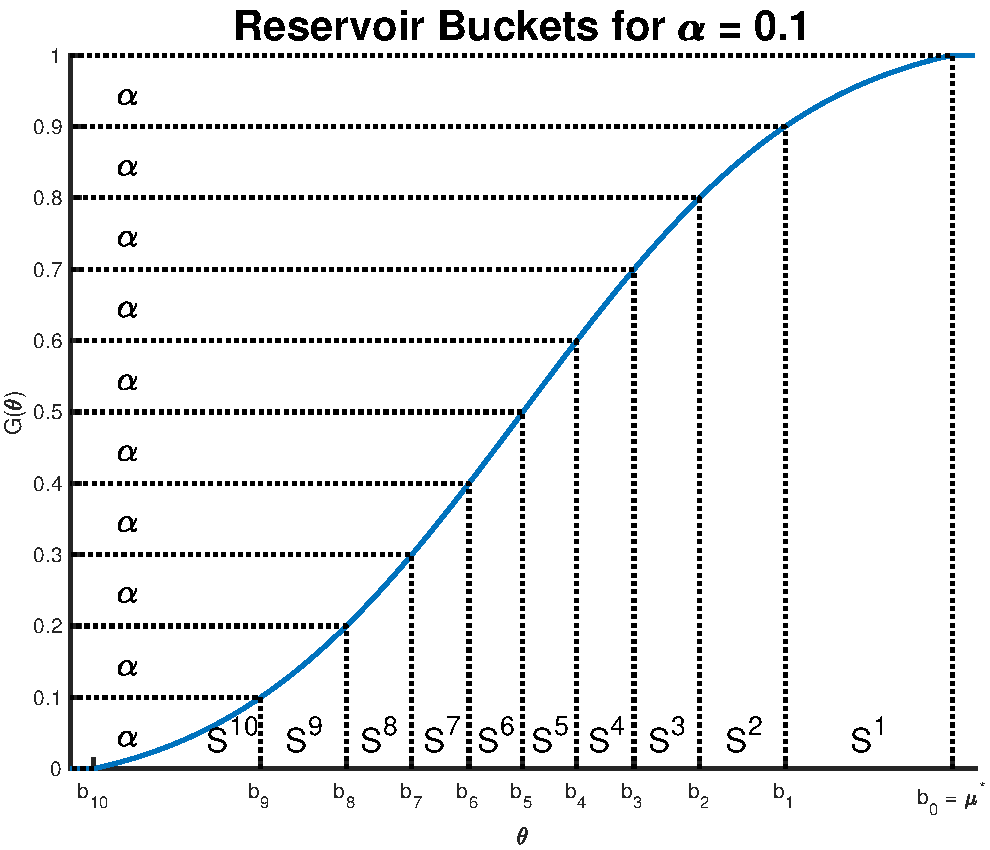
\includegraphics[width=0.35\textwidth]{fixedconfidence/figures/lb_buckets}
	\caption{Our reservoir partition.
		Each consecutive $\alpha$-interval on the CDF defines some
		subset $\ArmGrp{i}$.}
	\label{fig-lb-buckets}
	\vspace{-30pt}
\end{wrapfigure}

It also relies on the following partition of the arms in $\Arms$ by their
expected rewards.
Let $m = \lceil 1/\alpha \rceil$. We partition $\Arms$ into subsets
$\ArmGrp{i}$ for $1 \le i \le m$,
where $\ArmGrp{i} = \{\arm \in \Arms:\ArmMean(\arm) \in ]b_i,b_{i-1}]\}$.
The interval boundaries $b_i$ are defined so that each subset has measure
$\alpha$ under the reservoir distribution $\ExpRewardDensity$,
with the possible exception of the subset with smallest expected reward.
In particular, $b_0 = \ArmMean^*$ and $b_i$ lies at the boundary between subsets
$i$ and $i+1$.
\begin{align}
b_i = \left\{ \begin{array}{ll}
    \ArmMean^* & \text{if $i = 0$} \\
    \ExpRewardInvCDF(G(b_{i-1}) - \alpha) & \text{if $i \ge 1$}
\end{array}\right.,
\end{align}
where $\ArmMean^*$ is defined in Eq.~\ref{eq-mustar}.
See Figure~\ref{fig-lb-buckets} for an illustration.


%We now prove Theorem~\ref{thm-lb} under Assumptions~\ref{ass:kldiv} and \ref{ass:mu}, below.
In the
Bernoulli case,
Assumption~\ref{ass:mu} reduces to $\ArmMean^* < 1$ (no arm has perfect performance);
%while
% in the Gaussian, Exponential and Poisson
% case
when the set of possible
means $\ExpRewards$ is unbounded it always holds as $G$ has a finite
support.

\begin{assumption}\label{ass:mu} $\ArmMean^* < \sup_{\expReward \in \ExpRewards} \expReward$. 
 \end{assumption}


\begin{theorem}\label{thm-lb}
Fix some $\alpha, \delta \in ]0,1[$. Any $(\alpha,\delta)$-correct algorithm
needs an expected sample
complexity $\ETrueModel{\tau}$ that is lower bounded as follows.
\begin{align*}
\ETrueModel{\tau} \ge & \left(
    \frac{1}{\ArmKL{\ArmMean^*}{b_2}}
  + \sum_{i=2}^{m-1} \frac{1}{
            \ArmKL{b_i}{\ArmMean^*}
     }
\right)
\log \frac{1}{2.4\delta}.
\end{align*}
\end{theorem}

\begin{remark}\label{rem-finite-lb}
When $\Arms$ is finite s.t. $|\Arms|=K$, if we choose a uniform
reservoir and let
$\alpha = 1/K$, then $|\ArmGrp{i}| = 1$ for all $i$ and our lower bound
reduces to the bound obtained by \cite{JMLR15}
for best arm identification with $\epsilon=0$. Assuming arm means $\expReward_1 > \expReward_2 \geq \dots
\geq \expReward_K $, one has
\begin{align*}
\ETrueModel{T} \ge &\left[ \frac{1}{\ArmKL{\expReward_1}{\expReward_2}} +
\sum_{i=2}^K\frac{1}{\ArmKL{\expReward_i}{\expReward_1}}\right] \log
\frac{1}{2.4\delta}.
\end{align*}
\end{remark}






\subsubsection{Proof of Theorem~\ref{thm-lb}}

The proof relies on the following lemma that expresses a change of
measure in an infinite bandit model. Its proof is detailed in
Section~\ref{supp-proofs}. 

\begin{lemma}\label{lem-CD} Let $\ArmMeanAlt : \Arms \rightarrow \ExpRewards$ be an
alternative mean-mapping.
Let
$T_i(t) = \sum_{s=1}^t\1{\arm_s \in \ArmGrp{i}}$
be the number of times an arm in $\ArmGrp{i}$ has been
 selected.
For any stopping time $\sigma$ and
any
event $C \in H_\sigma$,
%
\vspace{-15pt}
%
\begin{align*}
\sum_{i=1}^m \ETrueModel{T_i(\sigma)} \sup_{\arm \in \ArmGrp{i}} \ArmKL{\ArmMean(\arm)}{\ArmMeanAlt(\arm)}
\geq  \BernKL{\PrTrueModel{C}}{\PrAltModel{C}},
\end{align*}
where $\BernKL{x}{y}=x\log(x/y) + (1-x)\log((1-x)/(1-y))$ is the Bernoulli relative
entropy.
\end{lemma}

Let $\tau^i = T_i(\tau)$ be the (random) number of draws from arms in 
$\ArmGrp{i}$,
so $\tau = \sum_{i=1}^m \tau^i$. Our lower bound on $\ETrueModel{\tau}$ follows
from
% individual 
bounds on each of the $\ETrueModel{\tau^i}$.
We omit $\ArmGrp{m}$ because its measure may be less than $\alpha$.
%
By Assumption~\ref{ass:mu}, there is $\epsilon>0$ such that $\ArmMean^* +
\epsilon < \sup_{\expReward\in \ExpRewards} \expReward$.
Fix $i$ between $2$ and $m-1$ and define an alternative arm reward mapping
$\ArmMeanAlt^i(\arm)$ as follows.
\begin{align}
\ArmMeanAlt^i(\arm) = \left\{
\begin{array}{ll}
\ArmMean^* + \epsilon & \text{if } \arm \in \ArmGrp{i} \\
\ArmMean(\arm) & \text{otherwise}
\end{array}
\right.
\end{align}

This
% alternative 
 mapping induces an alternative reservoir distribution $g^i$
under which for all $i < m$, 
$\GTargetNoEpsAlt = \ArmGrp{i}$ because
$\ArmGrp{i}$ has measure $\alpha$
(as $\ArmMeasure$ is unchanged)
and under $\ArmMeanAlt^i$ the expected rewards of its arms
are above all other arms by at least $\epsilon$.
Also, by construction $\GTargetNoEps = \ArmGrp{1}$.

Define the event $C_\ArmMean = (\hat{s}_\tau \in \ArmGrp{1})$. Any
$(\alpha,\delta)$-correct algorithm thus satisfies
$\PrTrueModel{ C_\ArmMean } \geq 1 - \delta$
and $\PrAltModel{ C_\ArmMean } \leq \delta$. 
First using some monotonicity properties of the binary
relative entropy $\BernKL{x}{y}$, one has 
%\begin{align*}
$
\BernKL{\PrTrueModel{C_\ArmMean}}{\PrAltModelI{C_\ArmMean}}
	\ge \BernKL{1-\delta}{\delta}
    \ge \log\frac{1}{2.4\delta},
$
%\end{align*}
where the second inequality is due to \cite{JMLR15}.

Applying Lemma~\ref{lem-CD} to event $C_\ArmMean$ and using the fact that
$\ArmMeanAlt^j(\arm)=\ArmMean(\arm)$ for all
$j\neq i$, one obtains
%
%\begin{align*}
$
 \ETrueModel{T^i}\sup_{\arm \in
\ArmGrp{i}} \ArmKL{\ArmMean(\arm)}{\ArmMean^*+\epsilon} \geq \log\frac{1}{2.4\delta}.
$
%\end{align*}
%
Letting $\epsilon$ go to $0$ yields, for all $i\neq 1$,
%
\begin{align*}
\ETrueModel{\tau^i} \ge \frac{1}{\sup_{\arm \in \ArmGrp{i}}
        \ArmKL{\ArmMean(\arm)}{\ArmMean^*}}
        \log\left(\frac{1}{2.4\delta}\right),
\end{align*}
%
and $\sup_{\arm \in \ArmGrp{i}}
\ArmKL{\ArmMean(\arm)}{\ArmMean^*} \leq \ArmKL{b_i}{\ArmMean^*}$ as $\expReward \mapsto \ArmKL{\expReward}{\ArmMean^*}$ is
decreasing when $\expReward < \ArmMean^*$.

We now define the alternative mean rewards mapping, for $\epsilon>0$ small
enough
\begin{align}
\ArmMeanAlt^1(\arm) = \left\{
\begin{array}{ll}
b_2 - \epsilon & \text{if } \arm \in \ArmGrp{1} \\
\ArmMean(\arm) & \text{otherwise}
\end{array}
\right.
\end{align}
One has $\GTargetNoEps=\ArmGrpEmp{1}$ whereas
$\GTargetNoEpsAltOne=\ArmGrpEmp{2}$, hence
letting $C_\ArmMean = (\hat{s}_\tau \in \ArmGrpEmp{1})$ satisfies
$\PrTrueModel{C_\ArmMean} \geq 1-\delta$ and $\PrAltModelOne{C_\ArmMean} \leq \delta$.
Using the same reasoning as before yields
\begin{align*}
\log\left(\frac{1}{2.4\delta}\right) \leq \ETrueModel{\tau^1} \sup_{\arm \in \ArmGrp{1}}
\ArmKL{\ArmMean(\arm)}{b_2-\epsilon}
= \ArmKL{\ArmMean^*}{b_2-\epsilon}
\end{align*}
Letting $\epsilon$ go to zero yields 
$\ETrueModel{\tau^1} \ge \displaystyle\frac{1}{\ArmKL{\ArmMean^*}{b_2}}\log\left(\frac{1}{2.4\delta}\right)$.
% \\ &= \frac{1}{\sup_{\arm \in
% \ArmGrp{2}} \ArmKL{\ArmMean(\arm)}{\ArmMean^*}}
%         \log\left(\frac{1}{2.4\delta}\right)
\qed
%\medskip

One can prove an $\epsilon$-relaxed version of this
theorem, which provides a
lower bound on the number of samples needed to
find an arm whose expected reward is within $\epsilon$ of the top-$\alpha$ 
fraction of arms with probability at least $1-\delta$.
When $\epsilon>0$ multiple subsets may contain such arms, and the 
proof approach above does not work for these subsets.
We instead adopt the strategy of
% the lower bound of 
\cite{Mannor04thesample}:
%using that 
at most one such subset can have 
probability greater than $1/2$ of its arms being chosen by the algorithm,
so we exclude this subset from our bound.
We arrive at the following, which holds when $\ArmMean^*+\epsilon$ is in $\ExpRewards$ (i.e. for $\epsilon$ small enough).
%
\begin{remark}
Fix some $\alpha, \epsilon, \delta \in ]0,1[$,
and let $q$ be the number of subsets containing arms within $\epsilon$ of the top $\alpha$ fraction.
Any $(\alpha,\epsilon,\delta)$-correct algorithm needs an expected sample
complexity $\ETrueModel{\tau}$ that is lower bounded as follows.
%
\vspace{-5pt}
%
\begin{align*}
\ETrueModel{\tau} \ge & \left(
    \frac{q - 1}{\ArmKL{b_1-\epsilon}{\ArmMean^*+\epsilon}}
  + \sum_{i=q + 1}^{m-1} \frac{1}{
            \ArmKL{b_i}{\ArmMean^*+\epsilon}
     }
\right)
\log \frac{1}{4\delta}.
\end{align*}
\end{remark}

\subsection{Algorithm and Upper Bound}\label{sec-fc-upper}

In this section we assume that $P_{\ExpRewards} = \Set{ p_{\expReward}, \expReward \in \ExpRewards }$ is a one-parameter exponential family, meaning that there exists some twice differentiable convex function $b(\expReward)$ and some reference measure $\nu$ such that $p_\expReward$ has a density $f_\expReward$ with respect to $\nu$, where 
%\[
$
f_\expReward(x) = \exp(\expReward x - b(\expReward)).
$
%\]
Distributions in an exponential family can indeed be parameterized by their means as $\ArmMean=b^{-1}(\expReward)$.
% Examples include the family of Bernoulli distributions, Gaussian distributions with a known variance, Poisson and Exponential distributions.
We do not make any new assumptions on the reservoir distribution.

Under these assumptions on the arms, we present and analyze 
a two-phase algorithm called
\texttt{$(\alpha,\epsilon)$-KL-LUCB}.
We prove the $(\alpha,\epsilon,\delta)$-correctness of this algorithm and a high
probability upper bound on its sample complexity in terms of the complexity of
the reservoir distribution induced by the arm measure $\ArmMeasure$ and the
arm reward mapping function $\ArmMean$.
We also show how to
%choose parameters to
obtain $(\alpha,\delta)$-correctness
under assumptions on the tail of the reservoir.


\subsubsection{The Algorithm}\label{kl-lucb}

\begin{figure}
\vspace{-5pt}
\fbox{
%\begin{minipage}{0.55\textwidth}
\begin{algorithm}[H]
\caption{$(\alpha,\epsilon)$-KL-LUCB}\label{alg-alpha-kl-lucb}
\begin{algorithmic}
\REQUIRE{$\alpha, \epsilon, \delta > 0$}
%\COMMENT{initialization}
\STATE{$n = \frac{1}{\alpha} \ln\frac{2}{\delta}$}
\FOR{$a \leftarrow 1$ \textbf{to} $n$}
    \STATE{draw arm $\arm^a \sim \ArmMeasure$}
    \STATE{sample arm $\arm^a$ once}
\ENDFOR
\STATE{$t = 1$ (current round number)}
\STATE{$B(n) = \infty$ (stopping index)}
\STATE{Compute confidence bounds $U_a(n)$ and $L_a(n)$}
%\COMMENT{\texttt{KL-LUCB}; run until confidence interval overlap is small}
\WHILE{$B(t) > \epsilon$}
	\STATE{Draw arm $\arm^{\hat{a}(t)}$ and $\arm^{\hat{b}(t)}$}
    \STATE{$t = t + 1$}
    \STATE{Update confidence bounds, compute $\hat{a}(t)$ and $\hat{b}(t)$}
	\STATE{$B(t) = U_{\hat{b}(t)}(t) - L_{\hat{a}(t)}(t)$}
\ENDWHILE
\STATE \textbf{return} {$w^{\hat{a}(t)}$}
\end{algorithmic}
\end{algorithm}
}
%\end{minipage}
\vspace{-5pt}
\end{figure}


\texttt{$(\alpha,\epsilon)$-KL-LUCB}, presented as Algorithm~\ref{alg-alpha-kl-lucb}, is a two-phase algorithm. It first queries $n=\frac{1}{\alpha} \log \frac{2}{\delta}$ arms
$\arm^1,\dots,\arm^n$ from $\ArmMeasure$, the measure over $\Arms$, and then runs the \texttt{KL-LUCB} algorithm \citep{COLT13} on the queried arms.
\texttt{KL-LUCB} identifies the $m$-best arms in a multi-armed bandit model, up to some $\epsilon>0$. We use it with $m=1$. 
This algorithm adaptively selects pairs of arms to sample from based on confidence intervals on the means of the arms. These confidence intervals rely on some 
exploration rate
%
\vspace{-5pt}
%
\begin{align}\label{explo-rate}
	\beta(t,\delta) := \log ( k_1 n t^\gamma / \delta ),
\end{align}
for
constants $\gamma>1$ and $k_1 > 2(1+\frac{1}{\gamma}-1)$. The upper and lower confidence bounds are
\begin{align} 
U_a(t) &:= \max \Set{ \expReward \in \ExpRewards : N_a(t) \ArmKL{\hat{p}_a(t)}{\expReward} \le \beta(t, \delta) }\label{kl-ub}\\
L_a(t) &:= \min \Set{ \expReward \in \ExpRewards : N_a(t) \ArmKL{\hat{p}_a(t)}{\expReward} \le \beta(t, \delta) }\label{kl-lb},
\end{align}
%
where $N_a(t) = \sum_{s=1}^t \1{\armRV_s = w^a}$ is the number of times arm $\arm^a$ was sampled by round $t$ and 
$\hat{p}_a(t) = \frac{1}{N_a(t)}\sum_{s=1}^t \1{\armRV_s = w^a}\rewardRV_s$
is the empirical mean reward of arm $\arm^a$ at round $t$, where $Z_s$ is an i.i.d. draw from arm $W_s$,
with distribution $p_{\ArmMean(W_s)}$.
Recall that $\ArmKL{\ArmMean_1}{\ArmMean_2}$ is the KL divergence between
arm distributions parameterized by their means $\ArmMean_1$ and $\ArmMean_2$.

For each queried arm $\arm^a$,
the algorithm maintains a confidence interval
$\ArmInterval = [L_a(t),U_a(t)]$
on $\ArmMean(w^a)$, and at any even round $t$ selects
two arm indexes: 
%\begin{itemize}[nosep]
 (1) the empirical best arm $\hat{a}(t) \in {\argmax}_{a=1,\dots,n} \ \hat{p}_a(t)$, and
(2) the arm among the empirical worst arms that is most likely to be mistaken with $\hat{a}(t)$, $\hat{b}(t) = {\argmax}_{a \neq \hat{a}(t)} \ U_a(t)$.
%\end{itemize}
The two arms are sampled: $\armRV_t = w^{\hat{a}(t)}$ and $\armRV_{t+1}=w^{\hat{b}(t)}$ and the confidence intervals are updated. 
The algorithm terminates when the overlap between the associated confidence intervals is smaller than some $\epsilon>0$: 
%\[
$
\tau = \inf\Set{t \in \N^* : L_{\hat{a}(t)}(t) > \max_{a \neq \hat{a}(t)} U_a(t) + \epsilon }.
$
%\]
The recommendation rule is $\hat{s}_\tau = w^{\hat{a}(t)}$.


%
% Correctness
%
\subsubsection{$(\alpha,\epsilon,\delta)$-Correctness}\label{sec-correctness}

For the algorithm to be $(\alpha,\epsilon,\delta)$-correct, it is sufficient that the following two events occur: 
\begin{itemize}[nosep]
    \item $A$ is the event that some $w^a$ was drawn from the
         top-$\alpha$ fraction of the reservoir.
    \item $B$ is the event that the \texttt{KL-LUCB} algorithm succeeds in 
identifying an arm within $\epsilon$ of the best arm among the $n$ arms drawn in the initialization
phase.
\end{itemize}
%
Indeed, on $A\cap B$ the recommended arm $\hat{s}_\tau = w^{\hat{a}(\tau)}$ satisfies 
%\[
$
\ArmMean(\hat{s}_\tau)  >  \max_{a} \ArmMean(w^a) - \epsilon  \geq  \ExpRewardInvCDF(1-\alpha) - \epsilon, 
$
%\]
hence $\hat{s}_\tau$ belongs to the top-$\alpha$ fraction, up to $\epsilon$. We prove in
Section~\ref{proof:correctness}
that $\Pr{A^\complement} \leq \delta/2$ and $\Pr{B^\complement}\leq \delta/2$,
which yields the following result. 
%
\vspace{-2pt}
%
\begin{lemma}\label{correctness}
With $\beta(t,\delta)$ defined in \eqref{explo-rate}, \texttt{$(\alpha,\epsilon)$-KL-LUCB} returns an arm from $\GTargetEps$
with probability at least $1-\delta$.
\end{lemma}
%
\vspace{-2pt}
%
It follows that when the parameter $\epsilon$ is chosen small
enough, e.g.,
%\begin{equation}
%\label{ass:epsilon}
$
\epsilon < \ExpRewardInvCDF\left(1 - \frac{\alpha}{2}\right) - \ExpRewardInvCDF\left(1 - {\alpha}\right),
$
%\end{equation}
\texttt{$(\alpha,\epsilon)$-KL-LUCB} is $(\alpha/2,\delta)$-correct.
For example, under the tail assumption~\ref{ass:smoothness}, $\epsilon$ can be 
chosen of order $c\alpha^{1/\beta}$.
%When the parameter $\beta$ is unknown, it can be estimated by, e.g., the
%algorithm of \cite{carpentier2015simple}. 
However, when nothing is known about the reservoir distribution (e.g. it may
not even be smooth) we are not aware of an algorithm to choose $\epsilon$
to provide a $(\alpha,\delta)$-correctness guarantee.


\subsubsection{Sample Complexity of \texttt{$(\alpha,\epsilon)$-KL-LUCB}}

Recall the partition of $\Arms$ into subsets $\ArmGrp{i}$ of measure
$\alpha$ for $1 \le i \le m$,
where $\ArmGrp{i} = \Set{\arm \in \Arms:\ArmMean(\arm) \in ]b_i,b_{i-1}]}$.
We define our sample complexity bound in terms of the complexity
term:
%
\vspace{-15pt}
%
\begin{align}
\overline{H}_{\alpha,\epsilon} =
    \frac{ 2 }{ \epsilon^2 } +
    \sum_{ i = 2 }^{m}\frac{1}{
    \max(\epsilon^2/2,\ArmCI{b_{i-1}}{b_1})},
\end{align}
%
%\vspace{-2pt}
%
where $\ArmCI{p}{q}$ is the Chernoff information
between two reward distributions parameterized by their means $p$ and $q$. This %information-theroretic 
quantity is closely related to the KL-divergence: it is defined as 
$\ArmCI{p}{q}=\ArmKL{z^*}{p}$ where $z^*$ is the unique solution in $z$ to $\ArmKL{z}{p} = \ArmKL{z}{q}$. 

Let the random variable $\tau$ be the number of samples used by
\texttt{$(\alpha,\epsilon)$-KL-LUCB}. The following upper bound on $\tau$ holds.

\begin{theorem}\label{samplecomp}
Let $\alpha,\delta$ such that $0<\delta \leq \alpha \leq 1/3$.
The \texttt{$(\alpha,\epsilon)$-KL-LUCB} algorithm with exploration rate
$\beta(t,\delta)$ defined by \eqref{explo-rate} and a parameter $\epsilon>0$
% satisfying condition \eqref{ass:epsilon}
is $(\alpha,\epsilon,\delta)$-correct and satisfies, with probability at least $1-7\delta$,
%
\vspace{-10pt}
%
\begin{align*}
    \tau \le 12 C_0(\gamma) \overline{H}_{\alpha,\epsilon}
    \log^2 \frac{1}{\delta} + o\left( \log^2 \frac{1}{\delta} \right),
\end{align*}
%
%\vspace{-2pt}
%
with $C_0(\gamma)$ such that
$C_0(\gamma) \ge \gamma \log(C_0(\gamma)) + 1 + \frac{\gamma}{e}$.
\end{theorem}

Theorem~\ref{samplecomp} only presents the leading term in $\delta$ (when $\delta$ goes to zero) of the sample complexity upper bound, but an explicit upper bound can be extracted from the proof of Theorem~\ref{samplecomp}, given in Section~\ref{sec-proof}.  
%We now compare this bound to our lower bound and discuss the squared log factor.

\subsection{Comparison and Discussion}
\label{sec-compare-lb-ub}

Our $\epsilon$-relaxed bounds simplify,
for appropriate constants $c_1,c_2$ and small enough $\epsilon$, to
\begin{align*}
\ETrueModel{ \tau } & \ge c_1 \left(
	\frac{1}{\ArmKL{b_1-\epsilon}{b_0+\epsilon}}
	+ \sum_{i=3}^{m-1} \frac{1}{\ArmKL{b_i}{b_0 + \epsilon}}
\right) \log \frac{1}{\delta},
\\
\tau &\le
c_2 \left( 
  \frac{4}{\epsilon^2}
  + \sum_{i=2}^{m-1} \frac{1}{\ArmCI{b_{i}}{b_1}}
\right) \log^2 \frac{1}{\delta}.
\end{align*}
A log factor separates our bounds,
and the upper bound complexity term is slightly
larger than that in the lower bound.
%\[\frac{1}{\ArmKL{\ArmMean^*}{b_2}} + \sum_{i=2}^m \frac{1}{\ArmKL{b_i}{\ArmMean^*}}.\]
KL-divergence in the lower bound is of comparable scale to Chernoff information in the upper bound:  in the Bernoulli case one has 
%\begin{align*}
$
\frac{(\ArmMean^*-x)^2}{2} < \ArmCI{x}{\ArmMean^*}
	< \ArmKL{x}{\ArmMean^*}
	< \frac{(\ArmMean^* - x)^2}{\ArmMean^*(1-\ArmMean^*)}.
$
%\end{align*}
However, for $i\neq 1$, $\ArmCI{b_i}{b_1}$ is slightly smaller than $\ArmKL{b_i}{b_0 + \epsilon}$,
while $\epsilon^2$ is smaller than $\ArmKL{b_1-\epsilon}{b_0+\epsilon}$. 
These differences are reduced as $\alpha$ is decreased.

When $\delta$ is not too small, the extra $\log \frac{1}{\delta}$ factor is small compared to the constants in our upper bound.
It is well-established 
for finite bandit models that for a wide variety of
%best-arm identification
algorithms the sample complexity 
scales like
$\log \frac{1}{\delta}$. The additional log factor comes from the fact that each phase of our algorithm needs a $\delta$-correctness
guarantee.
In our first phase, we choose a number of arms to draw from the reservoir
without drawing any rewards from those arms.
In the second phase, we observe rewards from our arms without drawing any new
arms from the reservoir.
It is an interesting open question to prove whether in any such two-phase algorithm the
$\log^2 \frac{1}{\delta}$ term is avoidable.
It is not hard to show that the first phase must draw at least $\frac{c}{\alpha} \log \frac{1}{\delta}$ arms for some constant $c$ in order to obtain a single arm from the top-$\alpha$ fraction with high probability, but the \emph{expected} number of arms in the top-$\alpha$ fraction is already $c \log \frac{1}{\delta}$ in this case.
The second phase can be reduced to a problem of finding one of the top $m$ arms, or of finding one arm above the unknown threshold $\ExpRewardInvCDF(1 - \alpha)$, but we are not aware of a lower bound on these problems even for the finite case.

Despite all this, it seems likely that a one-phase algorithm can avoid the
quadratic dependence on $\log \frac{1}{\delta}$.
Indeed, \cite{jamieson2016power}
provides such an algorithm for the special case of reservoirs involving just
two expected rewards.
They employ a subroutine which 
%is essentially a two-phase algorithm which
returns the target coin with constant probability
by drawing a number of coins that does not depend on $\delta$.
They wrap this subroutine in a $\delta$-correct algorithm which iteratively
considers progressively more challenging reservoirs,
terminating when
% as soon as 
a target coin is identified.
We agree with the authors that adapting this approach for general reservoirs is
an interesting research direction.
However their method relies on the special
shape of their reservoir
% in the two-coin setting
and it is not immediately clear how it might be generalized.


%\paragraph{Empirical results}
%
%%To our knowledge, there is no pure-exploration algorithm for the infinitely-armed bandit problem
%%in the fixed-confidence setting to compare \texttt{$(\alpha,\epsilon)$-KL-LUCB} with.
%We include empirical results of our performance in
%Appendix~\ref{sec-empirical}.
%Our algorithm not only identifies  an arm within $\epsilon$ of the top-$\alpha$
%fraction, but in fact it identifies a top-$\alpha$ arm the vast
%majority of the time for a variety of reservoir distributions.

%\small
%
%\paragraph{Acknowledgement.} We thank Virgil Pavlu for the fruitful discussions and his efforts that made this project better. E. Kaufmann acknowledges the support of the French Agence Nationale de la Recherche (ANR), under grant \texttt{ANR-16-CE40-0002} (project BADASS). 

\subsection{Empirical Results}\label{sec-empirical}

We exhibit
\texttt{$(\alpha,\epsilon)$-KL-LUCB} for infinite models of Bernoulli arms with
various parameter values.
In order to meet our assumption that $\ArmMean^* < 1$,
we truncate our $Beta$ distributions to have support on the
interval $]0, 0.95]$.
We report the fraction of runs in which it fails to find an arm within $\epsilon$ of the top-$\alpha$
fraction, the mean simple regret observed, and the mean budget used.

For the sake of computational efficiency we only update confidence intervals for those arms whose upper bounds overlap 
with the top lower bound. 

\begin{table}
%\captionsetup{justification=centering}
\caption{Performance of \texttt{$(\alpha,\epsilon)$-KL-LUCB}.
Mean of 100 runs.
``Effective $\alpha$'' gives the measure of arms meeting the $(\alpha,\epsilon)$
criteria.
``Errors'' indicates the fraction of runs where the $\alpha$
objective was not achieved; it should be below $\delta$.
\\
The budget $T$ is impacted roughly linearly by $1/\alpha$ and quadratically 
by $1/\epsilon$; the same regret is achieved with different budgets based
on parameter selection.
}
\label{tbl-results}
\vskip 0.15in
\begin{center}
\begin{small}
\begin{sc}
\begin{tabular}{lccc|cccc}
\hline
%\abovespace\belowspace
Reservoir & $\alpha$ & $\epsilon$ & $\delta$ & Effective $\alpha$ & Errors & Simple Regret & $T$ \\
\hline
Beta(1,1) & 0.025 & 0.024 & 0.05 & 0.049 & 0.00 & 0.008 & 51k \\
Beta(1,1) & 0.025 & 0.024 & 0.10 & 0.049 & 0.01 & 0.011 & 46k \\
Beta(1,1) & 0.050 & 0.010 & 0.05 & 0.060 & 0.02 & 0.015 & 113k \\
Beta(1,1) & 0.050 & 0.010 & 0.10 & 0.060 & 0.06 & 0.020 & 90k \\
Beta(1,1) & 0.050 & 0.048 & 0.05 & 0.098 & 0.00 & 0.014 & 12k \\
Beta(1,1) & 0.050 & 0.048 & 0.10 & 0.098 & 0.00 & 0.017 & 10k \\
Beta(1,1) & 0.050 & 0.050 & 0.05 & 0.100 & 0.01 & 0.014 & 11k \\
Beta(1,1) & 0.050 & 0.050 & 0.10 & 0.100 & 0.00 & 0.022 & 10k \\
Beta(1,1) & 0.100 & 0.010 & 0.05 & 0.110 & 0.02 & 0.030 & 71k \\
Beta(1,1) & 0.100 & 0.010 & 0.10 & 0.110 & 0.06 & 0.044 & 69k \\
Beta(1,1) & 0.100 & 0.050 & 0.05 & 0.150 & 0.00 & 0.037 & 10k \\
Beta(1,1) & 0.100 & 0.050 & 0.10 & 0.150 & 0.00 & 0.033 & 7k \\
Beta(1,2) & 0.025 & 0.063 & 0.05 & 0.221 & 0.00 & 0.044 & 10k \\
Beta(1,2) & 0.025 & 0.063 & 0.10 & 0.221 & 0.01 & 0.061 & 10k \\
Beta(1,2) & 0.050 & 0.010 & 0.05 & 0.234 & 0.03 & 0.075 & 79k \\
Beta(1,2) & 0.050 & 0.010 & 0.10 & 0.234 & 0.10 & 0.093 & 65k \\
Beta(1,2) & 0.050 & 0.050 & 0.05 & 0.274 & 0.01 & 0.069 & 10k \\
Beta(1,2) & 0.050 & 0.050 & 0.10 & 0.274 & 0.03 & 0.094 & 11k \\
Beta(1,2) & 0.050 & 0.091 & 0.05 & 0.314 & 0.01 & 0.077 & 5k \\
Beta(1,2) & 0.050 & 0.091 & 0.10 & 0.314 & 0.00 & 0.091 & 5k \\
Beta(1,2) & 0.100 & 0.010 & 0.05 & 0.326 & 0.04 & 0.123 & 63k \\
Beta(1,2) & 0.100 & 0.010 & 0.10 & 0.326 & 0.06 & 0.136 & 60k \\
Beta(1,2) & 0.100 & 0.050 & 0.05 & 0.366 & 0.00 & 0.113 & 10k \\
Beta(1,2) & 0.100 & 0.050 & 0.10 & 0.366 & 0.05 & 0.139 & 10k \\
Beta(1,3) & 0.025 & 0.076 & 0.05 & 0.368 & 0.00 & 0.132 & 12k \\
Beta(1,3) & 0.025 & 0.076 & 0.10 & 0.368 & 0.00 & 0.142 & 10k \\
Beta(1,3) & 0.050 & 0.010 & 0.05 & 0.378 & 0.01 & 0.176 & 87k \\
Beta(1,3) & 0.050 & 0.010 & 0.10 & 0.378 & 0.10 & 0.195 & 82k \\
Beta(1,3) & 0.050 & 0.050 & 0.05 & 0.418 & 0.00 & 0.166 & 13k \\
Beta(1,3) & 0.050 & 0.050 & 0.10 & 0.418 & 0.06 & 0.216 & 14k \\
Beta(1,3) & 0.050 & 0.096 & 0.05 & 0.464 & 0.00 & 0.183 & 7k \\
Beta(1,3) & 0.050 & 0.096 & 0.10 & 0.464 & 0.00 & 0.196 & 6k \\
Beta(1,3) & 0.100 & 0.010 & 0.05 & 0.474 & 0.06 & 0.233 & 69k \\
Beta(1,3) & 0.100 & 0.010 & 0.10 & 0.474 & 0.06 & 0.251 & 53k \\
Beta(1,3) & 0.100 & 0.050 & 0.05 & 0.514 & 0.01 & 0.220 & 10k \\
Beta(1,3) & 0.100 & 0.050 & 0.10 & 0.514 & 0.03 & 0.241 & 10k \\
\hline
\end{tabular}
\end{sc}
\end{small}
\end{center}
\vskip -0.1in
\end{table}


\subsection{Conclusion}\label{sec-conclusion}
%We have studied near-optimal arm identification for the infinitely-armed 
%bandit problem in the fixed confidence setting.
%We introduced new models within which to frame the problem and cast results.
In contrast with previous approaches to bandit models, we have
limited consideration to changes of distribution which change only the mean mapping 
$\ArmMean$ and not the measure $\ArmMeasure$ over arms $\Arms$.
This allows us to analyze infinite bandit models without a need to integrate
over the full reservoir distribution, so we can prove results for reservoirs
which are not even smooth.
We proved a lower bound on the sample complexity of the problem,
and we introduced an algorithm with an upper bound within a log factor of our
lower bound.

An interesting future direction is to study improved algorithms, namely
one-phase algorithms which alternate between sampling arms to estimate the 
reservoir and drawing new arms to obtain better arms with higher confidence.
These algorithms might be able to have only a $\log\frac{1}{\delta}$ instead of
$\log^2 \frac{1}{\delta}$ dependency in the upper bound.
In practice, however, the algorithm we present exhibits good empirical 
performance.

\newpage
%
%\appendix 

\subsection{Additional Proofs}\label{supp-proofs}

\subsubsection{Proof of Lemma~\ref{lem-CD}} \label{proof-CD}

We describe in this section the key results that allow us to adapt
\emph{changes of distribution} arguments to the infinite bandit setting.
Lemma~\ref{lem-CD} follows easily from Lemma~\ref{up-2014arXiv1407.4443K} and 
Lemma~\ref{main-lb-lemma} that are stated below and proved in the next two sections.

All the regret or sample complexity lower bounds in bandit models rely on
change of distributions arguments (see, e.g.
\cite{LaiRobbins85bandits,BurnKat96,Bubeck10BestArm}). A change of distribution
relates the probability of an event under a given bandit model to the
probability of that event under an alternative bandit model, that is ``not too
far'' from the initial model but under which the performance of the algorithm
is supposed to be completely different. \cite{Combes14Lip,JMLR15} recently
found an elegant formulation for such a change of distribution in terms of the
expected log-likelihood ratio and we explain below how we generalize these
tools to the infinite bandit model.

Given an infinite bandit model $(\ArmMeasure,\ArmMean)$, one may consider an alternative
bandit model $(\ArmMeasure,\ArmMeanAlt)$ in which the measure $\ArmMeasure$ is similar but the
mean function is different: $\ArmMeanAlt \neq \ArmMean$. As mentioned in
Section~\ref{setup}, we consider strategies such that
$\PrTrueModel{ \armRV_t | \historyRV_{T-1} }$ is independent from $\ArmMean$. Hence, defining the log-likelihood
ratio between $(\ArmMeasure,\ArmMean)$ and $(\ArmMeasure,\ArmMeanAlt)$ at round $t$ as
$L_{\ArmMean,\ArmMeanAlt}(t) = \log(\ell(\historyRV_t ; \ArmMean,\ArmMeasure) / \ell(\historyRV_t; \ArmMeanAlt,\ArmMeasure))$, where the likelihood is defined in 
\eqref{Likelihood}, one has 
\begin{align}
L_{\ArmMean,\ArmMeanAlt}(T)
    &= \sum_{t=1}^T \log \frac{f_{\ArmMean(\armRV_t)}(\rewardRV_t)}{f_{\ArmMeanAlt(\armRV_t)}(\rewardRV_t)}.\label{logLikelihood}
\end{align}

The following result generalizes Lemma 1 in \cite{JMLR15} to the infinite
bandit model. It permits to relate the expected log-likelihood ratio to the
probability of any event under the two different models.

\begin{lemma}\label{up-2014arXiv1407.4443K}
\label{lem-log-lik}
Let $\sigma$ be a stopping time and $\ArmMean$ and $\ArmMeanAlt$ be two reward mappings.
For any event $C$ in $H_\sigma$,
\begin{align*}
\ETrueModel{ L_{\ArmMean,\ArmMeanAlt}(\sigma) }
	\ge \BernKL{\PrTrueModel{C}}{\PrAltModel{C}},
\end{align*}
where $\BernKL{x}{y}=x\log(x/y) + (1-x)\log((1-x)/(1-y))$ is the Bernoulli relative
entropy.
\end{lemma}

The next result provides an upper bound on the expected log-likelihood ratio.
While in a classic multi-armed bandit model, the log-likelihood can be
expressed as a sum that features the expected number of draws of each arm, such
a quantity would not be defined in the infinite bandit model. Hence, we need to
introduce a partition of $\Arms$.

\begin{lemma}\label{main-lb-lemma}
Fix $\ArmGrpEmp{1},\dots,\ArmGrpEmp{m}$ a partition of $\Arms$ and let
$T_i(t) = \sum_{s=1}^t\1{\arm_s \in \ArmGrp{i}}$
be the number of times an arm in $\ArmGrp{i}$ has been selected.
For any stopping time $\sigma$,
\begin{align*}
\ETrueModel{ L_{\ArmMean,\ArmMeanAlt}(\sigma) }
\leq \sum_{i=1}^m \ETrueModel{ T_i(\sigma) } \sup_{\arm \in \ArmGrp{i}} \ArmKL{\ArmMean(\arm)}{\ArmMeanAlt(\arm)}.
\end{align*}
\end{lemma}



\subsubsection{Proof of Lemma~\ref{up-2014arXiv1407.4443K}}

The proof for the infinite case follows the argument by \cite{JMLR15} for the
finite case. First, the conditional Jensen's inequality is applied, given the
convexity of
$\exp(-x)$.
The expectation derivations hold for our infinite arms case without
modification.
The only necessary statement for which the finite case proof needs updating,
$\PrAltModel{C} = \ETrueModel{ \1{C} \exp(-L_{\ArmMean,\ArmMeanAlt}(\sigma)) }$,
is proven for our infinite case setting as Lemma~\ref{lem-pr-exp}.


\begin{lemma}\label{lem-pr-exp}
Let $\ArmMean$ and $\ArmMeanAlt$ be two arm reward mappings,
$L_{\ArmMean,\ArmMeanAlt}(T)$ be the log likelihood ratio defined in \eqref{logLikelihood}
and $C$ be an (event) subset of histories of length $T$.
Then
\begin{align*}
\PrAltModel{C}
	= \ETrueModel{ \1{C} \cdot \exp(-L_{\ArmMean,\ArmMeanAlt}(T)) }
\end{align*}
\end{lemma}

\paragraph{Proof of Lemma~\ref{lem-pr-exp}.}
Let $\ell(\historyRV_T ;\ArmMean,\ArmMeasure)$ be the likelihood function defined in \eqref{Likelihood}.
We introduce furthermore the notation $h_t = (\armRV_1,\rewardRV_1,\dots,\armRV_t,\rewardRV_t)$, $\bm \arm_T=(\armRV_1,\dots,\armRV_T)$ and $\bm z_T =(\rewardRV_1,\dots,\rewardRV_T)$. Recall that a strategy is such that conditional density of $\armRV_t$ given $\historyRV_{t-1}$ does not depend on the mean reward mapping but only on the reservoir distribution: we denote it by $\PrNone_\ArmMeasure(\armRV_t | \historyRV_{t-1})$.
The proof of Lemma~\ref{lem-pr-exp} follows from the following inequalities. 
\begin{align*}
\PrAltModel{C} =
  \EAltModel{ \1{C} }
 & =  \int \1{C}(\historyRV_T) \ell(\historyRV_T; \ArmMeanAlt, \ArmMeasure) \diff \historyRV_T \\
 & = \int \1{C}(h_T)
 \prod_{t=1}^Tf_{\ArmMeanAlt(\armRV_t)}(\rewardRV_t)
 \PrNone_\ArmMeasure(\armRV_t | h_{t-1}) \diff \bm \arm_T  \diff \bm z_T \\
 & = \int \1{C}(h_T)
 	\prod_{t=1}^T\frac{f_{\ArmMeanAlt(\armRV_t)}(\rewardRV_t)}{f_{\ArmMean(\armRV_t)}(\rewardRV_t)} \prod_{t=1}^T f_{\ArmMean(\armRV_t)}(\rewardRV_t)
 \PrNone_{\ArmMeasure}(\armRV_t | h_{t-1}) \diff \bm \arm_T \diff \bm z_T \\
  & = \int \1{C}(H_T) \prod_{t=1}^T\frac{f_{\ArmMeanAlt(\armRV_t)}(\rewardRV_t)}{f_{\ArmMean(\armRV_t)}(\rewardRV_t)} \ell(\historyRV_T;\ArmMean,\ArmMeasure) \diff \historyRV_T  \\
  & = \ETrueModel{
 \1{C} \cdot\prod_{t=1}^{T} \frac{ f_{\ArmMeanAlt(\armRV_t)}(\rewardRV_t) }{ f_{\ArmMean(\armRV_t)}(\rewardRV_t) } }.
\end{align*}
\qed



\subsubsection{Proof of Lemma~\ref{main-lb-lemma}}

The proof follows from the following inequalities.
\begin{align*}
& \ETrueModel{ L_{\ArmMean,\ArmMeanAlt}(\sigma) } \\
&= \ETrueModel{ \sum_{t=1}^\infty
	\ETrueModel{ \left.\1{\sigma \geq t-1} \log
	\frac{f_{\ArmMean(\armRV_t)}(\rewardRV_t)}{f_{\ArmMeanAlt(\armRV_t)}(\rewardRV_t)} \right|
	\historyRV_{t-1}}}\\
& = \ETrueModel{ \sum_{t=1}^\infty \1{\sigma \geq t-1}
\ArmKL{\ArmMean(\armRV_t)}{\ArmMeanAlt(\armRV_t)}} \\
& \leq  \ETrueModel{ \sum_{i=1}^m \sum_{t=1}^\sigma \1{\armRV_t \in \ArmGrp{i}}
\sup_{\arm \in \ArmGrp{i}} \ArmKL{\ArmMean(\arm)}{\ArmMeanAlt(\arm)} }
\end{align*}


\subsubsection{Proof of Lemma~\ref{correctness}}\label{proof:correctness}

Letting
\begin{align*}
A & =  \left(\exists a \leq n : \ArmMean(w^a) > \ExpRewardInvCDF(1-\alpha)\right) \\
B & =  \left(\ArmMean_{\hat{a}(\tau)} \geq \max_{a} \ArmMean_a - \epsilon\right),
\end{align*}
Lemma~\ref{correctness} follows from the fact that $\Pr{A^\complement}\leq \frac{\delta}{2}$ and $\Pr{B^\complement} \leq \frac{\delta}{2}$, that we now prove. 

First, by definition of the reservoir distribution $G$ and the fact that $\ArmMean(\armRV^t)$ are i.i.d. samples from it, one has

\begin{align*}
 \Pr{A^\complement} & =  \Pr{\bigcap_{a = 1}^n\left( \ArmMean(\arm^a) \leq \ExpRewardInvCDF(1-\alpha)\right)}
 	= \left(1 - \alpha \right)^n \\
 & =  \exp\left(-n\log\left(\frac{1}{1- \alpha}\right)\right) \\
 & =  \exp\left(-\log\left(\frac{2}{\delta}\right)\frac{1}{\alpha}\log\left(\frac{1}{1- \alpha}\right)\right) \leq \frac{\delta}{2},
\end{align*}
using that $-\log(1-x)>x$. 

The upper bound on $\Pr{B^\complement}$ follows the same lines as that of the correctness of the \texttt{KL-LUCB} algorithm \citep{COLT13}, however note that we are able to use a smaller exploration rate compared to this work.
	Abusing notation slightly we let $\ArmMean_a := \ArmMean(\arm^a)$,
	and letting $(1) = \argmax_a \ArmMean_a$ we have
\begin{align*}
 B^\complement & \subseteq  (\exists t \in \N : \ArmMean_{(1)} > U_{(1)}(t)) \!\!\!\!\!\bigcup_{a : \ArmMean_a < \ArmMean_{(1)} - \epsilon} \!\!\!\!\!\!\!\! (\exists t \in \N: L_a(t) > \ArmMean_a).
\end{align*}
Let $\operatorname{d}^-(x,y) := \ArmKL{x}{y}\1{x > y}$.
For each $a$, $\Pr{\exists t\in \N: L_a(t) > \ArmMean_a | \ArmMean_a}$ is upper bounded by
\begin{align*}
&\Pr{ \exists t \in \N : N_a(t) \operatorname{d}^-(\hat{p}_a(t),\ArmMean_a) > \beta(t,\delta) } \\
& \leq   \Pr{ \exists t \in \N : N_a(t) \operatorname{d}^-(\hat{p}_a(t),\ArmMean_a) > \beta(N_a(t),\delta) } \\
& \leq   \Pr{ \exists s \in \N : s \operatorname{d}^-(\hat{p}_a(t),\ArmMean_a) > \beta(s,\delta) } \\
& \leq  \sum_{s=1}^\infty \exp(-\beta(s,\delta)) \leq \frac{\delta}{k_1 n}\sum_{t=1}^\infty \frac{1}{t^\gamma} \leq \frac{\delta}{2n},
\end{align*}
where we use a union bound together with Chernoff's inequality and the fact that $k_1$ is chosen to be larger than $2 \sum_{t}\frac{1}{t^\gamma}$. Similar reasoning shows that
\begin{align*}
\Pr{\exists t \in \N : \ArmMean_{(1)} > U_{(1)}(t)}
	\leq \frac{\delta}{2n},
\end{align*}
and a union bound yields $\Pr{B^\complement} \leq \frac{\delta}{2}$.

\subsubsection{Proof of Lemma~\ref{lem-armNumAppBandit}}\label{proof:armNumAppBandit}

For every $i$, let $\cR_i$ be the set of arms $a \in \{1,\dots,n\}$ such that $w^a \in \ArmGrp{i}$. Letting $Y^i_a = \1{w^a \in \ArmGrp{i}}$, as $\ArmMeasure(\ArmGrp{i}) = \alpha$, $(Y^i_a)_a$ is i.i.d. with a Bernoulli distribution of parameter $\alpha$ and 
$|\cR_i| = \sum_{a=1}^n Y^i_a$. 

Using Chernoff's inequality for Bernoulli random variables yields 
\begin{align*}
 &\Pr{ |\cR_i| > 6 \log(1/\delta) }
 	= \Pr{ |\cR_i| > 3\alpha n } \\
 & =  \Pr{ \frac{1}{n}\sum_{a=1}^n Y^i_a > 3\alpha }
 	\leq \exp\left\{-n\BernKL{3\alpha}{\alpha}\right\},
\end{align*}
where $\BernKL{x}{y}=x\log(x/y) + (1-x)\log((1-x)/(1-y))$ is the binary relative entropy. 

Using Lemma~\ref{lem-ineq-kl} below for $\beta=2$, if $\alpha \leq 1/3$ it holds that
\begin{align*}
\BernKL{3\alpha}{\alpha} \geq (3\log 3 - 2)\alpha > \alpha
\end{align*}
and, using again the definition of $n$,
\begin{align*}
 &\Pr{ |\cR_i| > 6 \log(1/\delta) }
 	\leq \exp\left\{- 2 \log(1/\delta)\right\}
 	= \delta^2.
\end{align*}
Using a union bound on the $m$ subsets $\ArmGrp{i}$, and the fact that $m \leq 1/\alpha$ and $\delta \leq \alpha$, one has 
\begin{align*}
\Pr{ C^\complement }
	\leq m \delta^2
	\leq \frac{\delta^2}{\alpha}
	\leq \delta,
\end{align*}
which concludes the proof.

\begin{lemma}\label{lem-ineq-kl} Let $\beta > -1$. For all $\alpha \leq \frac{1}{1+\beta}$, 
\begin{align*}
\BernKL{(1+\beta)\alpha}{\alpha}
	\geq ((1+\beta)\log(1+\beta) - \beta) \alpha.
\end{align*}
\end{lemma}

This inequality is optimal in the first order in the sense that its two members are equivalent when $\alpha$ goes to zero.

\paragraph{Proof of Lemma~\ref{lem-ineq-kl}.} By definition
\begin{align*}
 \BernKL{(1+\beta)\alpha}{\alpha}
 	=& (1+\beta)\alpha\log(1+\beta) \\
 & + (1-(1+\beta)\alpha)\log\left(\frac{1-(1+\beta)\alpha}{1-\alpha}\right) \\
 =& (1+\beta)\alpha\log(1+\beta) \\
  &  +  (1-(1+\beta)\alpha)\log\left(1 - \frac{\beta\alpha}{1-\alpha}\right) 
\end{align*}
Now, using the fact that $1 - (1-\beta)\alpha >0$ for $\alpha \leq 1/(1+\beta)$ and the following inequality 
\[\forall x > -1, \ \ \log(1+x) \geq \frac{x}{1+x}\]
one obtains 
\begin{align*}
	\BernKL{(1+\beta)\alpha}{\alpha}
		\geq & (1+\beta)\alpha\log(1+\beta)
\\
   &  +  (1-(1+\beta)\alpha)\frac{-\beta\alpha}{1-\alpha - \beta\alpha}
\\
  = & \alpha \left((1+\beta)\log(1+\beta) - \beta\right)
\end{align*}
\qed


\subsubsection{Proof of Theorem~\ref{samplecomp}} \label{sec-proof}

We let $\ArmMean_a := \ArmMean(\arm^a)$ and
denote by $\bm\ArmMean = (\ArmMean_1,\dots,\ArmMean_n)$ the means of the $n$ arms that have been queried, sorted in decreasing order. 

In addition to events $A$ and $B$ defined in Section~\ref{sec-correctness}, we introduce the event $C$ that for every subset $i \leq m$, at most $6\log\frac{1}{\delta}$
        arms belong to $\ArmGrp{i}$:
\begin{align}
C = \bigcap_{i = 1,\dots,m} \left\{|\{ a \leq n : w^a \in \ArmGrp{i}\}| \leq 6\log({1}/{\delta})\right\}
\end{align}
We prove the following in
Section~\ref{proof:armNumAppBandit}.

\begin{lemma}\label{lem-armNumAppBandit} If $\delta \leq \alpha \leq 1/3$,
$\Pr{ C } \geq 1-\delta$.
\end{lemma}

For all $t\in\N$ we introduce the event 
\begin{align}
W_t = \bigcap_{1\leq a \leq n} (L_a(t) \leq \ArmMean_a \leq U_a(t))
\end{align}
and define $W = \cap_{t\in\N^*} W_t$. By the same argument as the one used in the proof of Lemma~\ref{correctness} (see
Section~\ref{proof:correctness}),
one 
can show that $\Pr{ W } \geq 1-2\delta.$

Fix $c \in [\ArmMean_2,\ArmMean_1]$. Our analysis relies on the following crucial statement.

\begin{proposition}[\cite{COLT13}]\label{kauffprop}Let
$\tilde{\beta}_a(t) := \sqrt{ \frac{\beta(t,\delta)}{2 N_a(t)} }$. If $W_t$ holds and $(U_{\hat{b}(t)} - L_{\hat{a}(t)}>\epsilon)$ then there exists $a\in \{\hat{a}(t),\hat{b}(t)\}$ such that
\begin{align}
c \in \ArmInterval \text{ and } \tilde{\beta}_a(t) > {\epsilon}/{2}.
\end{align}
\end{proposition}
%
Fixing some integer $T \in \N$, we now upper bound $\tau$ on the event $\cE := A\cap B\cap C\cap W$.
\begin{align*}
& \min(\tau,T)   \le  \sum_{t=1}^T\1{\tau > t} = n + 2\sum_{\substack{t  \in n + 2\N\\t \leq T}}\1{\tau > t} \\
& \leq  n + 2\sum_{\substack{t  \in n + 2\N\\t \leq T}}\1{U_{\hat{b}(t)} - L_{\hat{a}(t)} > \epsilon} \\
& \leq  n + 2\sum_{\substack{t  \in n + 2\N\\t \leq T}}\1{\exists a \in \{\hat{a}(t),\hat{b}(t)\}: c \in \ArmInterval, \tilde{\beta}_a(t) > \epsilon/2},
\end{align*}
using Proposition~\ref{kauffprop} and the fact that W holds. To ease the notation, we let $\ArmGrpEmp{t} = \{\hat{a}(t),\hat{b}(t)\}$ be the set of drawn arms at round $t$. Letting $\EpsCheapArms=\Set{a : \ArmCI{\ArmMean_a}{c} < \epsilon^2/2}$ and noting that $\tilde{\beta}_a(t) > \epsilon/2 \iff N_a(t) <
\beta(t,\delta)/(\epsilon^2/2)$, 
\begin{align*}
& \min(\tau,T)   \le  n + 2\!\sum_{a \in \EpsCheapArms}\!\sum_{\substack{t  \in n + 2\N\\t \leq T}}\!\!\! \1{a \in \ArmGrpEmp{t}}\1{N_a(t) < \beta(T,\delta)/(\epsilon^2/2)}\\
&  \hspace{1cm}+ 2\sum_{a \in \EpsCheapArms^\complement} \sum_{\substack{t  \in n + 2\N\\t \leq T}} \1{a \in \ArmGrpEmp{t}}\1{N_a(t)\ArmKL{\hat{p}_a(t)}{c} \leq \beta(T,\delta))}
\end{align*}
Now defining the event
\begin{align*}
G_T^a = \!\!\!\!\!\bigcup_{\substack{t  \in n + 2\N\\t \leq T}}\!\! \left\{\!N_a(t) > \! \frac{\beta(T,\delta)}{\ArmCI{\ArmMean_a}{c}} , N_a(t)\ArmKL{\hat{p}_a(t)}{c} \! \leq\!  \beta(T,\delta) \!\right\}
\end{align*}
From Lemma 1 in \cite{COLT13},
\begin{align}
\Pr{ G_T^a | \bm\ArmMean }
	\leq \frac{1}{\ArmCI{\ArmMean_a}{c}}\exp(-\beta(T,\delta)).\label{boundE1}
\end{align}
Introducing $\cF_T = \cap_{a \in \EpsCheapArms^\complement} (G_T^a)^\complement$, one can further upper bound $\tau$ on $\cE \cap \cF_T$ as 
\begin{align*}
& \min(\tau,T)   \le  n + 2\!\sum_{a \in \EpsCheapArms}\!\sum_{\substack{t  \in n + 2\N\\t \leq T}}\!\!\!\! \1{a \in \ArmGrpEmp{t}}\1{N_a(t) < \beta(T,\delta)/(\epsilon^2/2)}\\
&  \hspace{1cm}+  2\sum_{a \in \EpsCheapArms^\complement} \sum_{\substack{t  \in n + 2\N\\t \leq T}} \1{a \in \ArmGrpEmp{t}}\1{N_a(t) < \beta(T,\delta)/\ArmCI{\ArmMean_a}{c}} \\
& \hspace{1cm} \le  n + 2\underbrace{\left[\sum_{a \in \EpsCheapArms} \frac{2}{\epsilon^2} + \sum_{a \in \EpsCheapArms^\complement}\frac{1}{\ArmCI{\ArmMean_a}{c}}\right]}_{=: H(\bm\ArmMean,c,\epsilon)}\beta(T,\delta).
\end{align*}
We now provide a deterministic upper bound on $H(\bm\ArmMean,c,\epsilon)$, by summing over the arms in the different subsets $\ArmGrp{i}$.
Let $q$ be the number of subsets containing arms within $\EpsCheapArms$.
We choose $c$ such that $c>\ExpRewardInvCDF(1-\alpha) = b_1$ (such a choice is possible as $\ArmMean_1 >\ExpRewardInvCDF(1-\alpha)$ as event $A$ holds) and note that
	$\EpsCheapArms \subseteq \cup_{i\le q} \ArmGrpEmp{i}$.
One has 
\begin{eqnarray*}
H(\bm \ArmMean,c,\epsilon)
	\!\!& \leq &\!\!\!\!\!
	\sum_{i=1}^q
	\sum_{a : \arm_a \in \ArmGrp{i}} \frac{2}{\epsilon^2}
	+
	\sum_{i=q+1}^m
	\sum_{a : \arm_a \in \ArmGrp{i}}
	\!\!\frac{1}{\ArmCI{\ArmMean_a}{\ExpRewardInvCDF(1-\alpha)}}  \\
& \leq &\!\! 6 \overline{H}_{\alpha,\epsilon}\log(1/\delta),
\end{eqnarray*}
using that event $C$ holds and each $\ArmGrp{i}$ contains at least $6\log(1/\delta)$ arms. Hence on $\cE \cap \cF_T$, 
\[\min(\tau,T)   \le n + 12 \overline{H}_{\alpha,\epsilon}\log(1/\delta) \beta(T,\delta).\]
Applying this to  $T=T^*$ where 
\[T^* := \inf\{ T \in \N : n + 12 \overline{H}_{\alpha,\epsilon}\log(1/\delta) \beta(T,\delta) \leq T\},\]
one obtains $\min(\tau,T) \leq T$, hence $\tau \leq T$. We proved that 
\begin{align*}
\Pr{ \tau \leq T^* }
	\leq 1 - 4\delta - \Pr{ \cF_{T^*}^\complement }.
\end{align*}

An upper bound on $T^*$ can be extracted from Appendix E of \cite{COLT13}: 
\begin{align*}
T^* \leq 12C_0(\gamma)\overline{H}_{\alpha,\epsilon}\log\frac{1}{\delta} \log\left(\frac{12k_1n(\log(1/\delta)^\gamma)\overline{H}_{\alpha,\epsilon}^\gamma}{\delta}\right) + n.
\end{align*}
An upper bound on $\Pr{ \cF_{T^*}^\complement }$ concludes the proof: 
\begin{align*}
 \Pr{ \cF_{T^*}^\complement }
 	&\leq  2\delta + \Pr{ \cF_{T^*}^\complement \cap A \cap C } \\
	&= 2\delta + \EIN{ \Pr{ \cF_{T^*}^\complement | \bm \ArmMean } \1{A \cap C} }
\end{align*}
Now, on $A\cap C$ (which is used for the second inequality), using \eqref{boundE1},
\begin{align*}
 \Pr{ \cF_{T^*}^\complement | \bm \ArmMean }
 	&\leq \sum_{a \in \EpsCheapArms^\complement}
 		\frac{1}{\ArmCI{\ArmMean_a}{c}}\exp(-\beta(T^*,\delta)) \\
	&\leq 6\overline{H}_{a,\epsilon}\log(1/\delta)\exp(-\beta(T^*,\delta)) \\
	&\leq \left(\frac{6\overline{H}_{a,\epsilon}\log(1/\delta)}{k_1 n (T^*)^\gamma}\right)  \delta \leq \delta,
\end{align*}
where the last inequality follows from the definition of $T^*$. Thus $\Pr{ \cF_{T^*}^\complement } \leq 3\delta$.

\newpage
\section{The Fixed Budget Setting}\label{fixedbudget}

%%\usepackage[margin=1.5in]{geometry}
%
%% \usepackage{algorithm2e}
%% \usepackage{enumitem}
%% \usepackage{filecontents}
%% \usepackage{todonotes}
%% \usepackage{graphicx}
%\usepackage{subcaption}
%% \usepackage{longtable}
%% \usepackage{booktabs}
%\usepackage{wrapfig}
%% \usepackage[numbers]{natbib}
%%\usepackage{algorithm}
%%\usepackage{algorithmic}
%
%\usepackage{amsmath,amssymb,amsfonts,bm,url,dsfont,hyperref,color}
%%\usepackage[margin=1in]{geometry}
%\newcommand{\kevin}[1]{{\textcolor{red}{#1}}}
%\newcommand\tab[1][1cm]{\hspace*{#1}}
%\newcommand{\polylog}{{\rm polylog}}
%
%\def\calD{\mathcal{D}}
%\def\calE{\mathcal{E}}
%\def\H{\mathcal{H}}
%\def\calS{\mathcal{S}}
%\def\calI{\mathcal{I}}
%\def\S{\mathcal{S}}
%\def\A{\mathcal{A}}
%\def\E{\mathbb{E}}
%\def\1{\mathbf{1}}
%\def\P{\mathbb{P}}
%\def\R{\mathbb{R}}
%\def\mualpha{\mu^{(\alpha)}}
%\newcommand{\mc}[1]{\mathcal{#1}}
%\newcommand{\mbb}[1]{\mathbb{#1}}
%\newcommand{\mbf}[1]{\mathbf{#1}}
%
%%\newtheorem{theorem}{Theorem}
%%\newtheorem{lemma}{Lemma}
%%\newtheorem{remark}{Remark}
%\newtheorem{assumption}{Assumption}
%%\newtheorem{definition}{Definition}

%\setlength{\parindent}{0in}
%\setlength{\parskip}{.5em}

% Heading arguments are {volume}{year}{pages}{date submitted}{date published}{paper id}{author-full-names}

%\jmlrheading{1}{2000}{1-48}{9/18}{10/00}{aziz18a}{Maryam Aziz and Kevin Jamieson and Javed Aslam}
%
%% Short headings should be running head and authors last names
%
%\ShortHeadings{Pure-Exploration for Infinite-Armed Bandits with General Reservoirs}{Aziz, Jamieson, Aslam}
%\firstpageno{1}

%\usepackage[utf8]{inputenc}

%\begin{document}

%\title{Pure-Exploration for Infinite-Armed Bandits with General Arm Reservoirs}

%\author{\name Maryam Aziz \email azizm@ccs.neu.edu \\
%\addr College of Computer and Information Sciences \\
%Northeastern University \\
%Boston, MA 02115, USA
%\AND
%\name Kevin Jamieson \email jamieson@cs.washington.edu \\
%\addr Paul G. Allen School of Computer Science \& Engineering \\
%University of Washington \\
%Seattle, WA 98195, USA
%\AND
%\name Javed Aslam \email jaa@ccs.neu.edu \\
%\addr College of Computer and Information Sciences \\
%Northeastern University \\
%Boston, MA 02115, USA 
%}
%
%\editor{}
%
%
%\maketitle

%\begin{abstract}%   <- trailing '%' for backward compatibility of .sty file
We consider a muti-armed bandit game where the number of arms is much larger than the maximum budget and is effectively infinite.
We characterize necessary and sufficient conditions on the total budget for an algorithm to return an $\epsilon$-good arm with probability at least $1-\delta$.
In such situations, the sample complexity depends on $\epsilon, \delta$ and the so-called reservoir distribution $\nu$ from which the means of the arms are drawn iid. 
While a substantial literature has developed around analyzing specific cases of $\nu$ such as the beta distribution, our analysis makes no assumption about the form of $\nu$.
Our algorithm is based on successive halving with the surprising exception that arms start to be discarded after just a single pull, requiring an analysis that goes beyond concentration alone. 
The provable correctness of this algorithm also provides an explanation for the empirical observation that the most aggressive bracket of the Hyperband algorithm of \cite{li2017hyperband} for hyperparameter tuning is almost always best.    
%\end{abstract}

%\begin{keywords}
%  Infinite-armed bandit, pure-exploration, best-arm identification
%\end{keywords}

% In Section~\ref{experiments} we discuss our  experimental results of using \texttt{Sequential Halving} for pure exploration of the infinitely armed bandits and in Section~\ref{theory} we analyze the simple regret of the algorithm.
%!TEX root = main.tex

\subsection{Introduction}\label{intro}
Consider a multi-armed bandit problem with $n$ arms where the $j$th pull from the $i$th arm emits an independent random variable $X_{i,j} \in [0,1]$ with $\mu_i:=\E[X_{i,j}]$. 
Given $\epsilon,\delta \in (0,1)$, how many total pulls must an algorithm make in order to return an arm $\widehat{i} \in \{1,\dots,n\}$ with a \emph{small}\footnote{While non-standard in stochastic bandits, seeking small means significantly simplifies notation in the infinite-armed bandit setting; we translate all prior results to this equivalent perspective.} mean that satisfies $\mu_{\widehat{i}} \leq \displaystyle\min_{j} \mu_j + \epsilon$ with probability at least $1-\delta$?
Much effort has gone into answering this and closely related questions resulting in a rich collection of algorithms.
But each algorithm starts the same:  \textit{Pull each arm $i \in \{1,\dots,n\}$ once.}
% \begin{quote}

% \centerline{}
% \end{quote}
%
%
\begin{wrapfigure}{r}{0.45\textwidth}
% \vspace{-2.5em}
\includegraphics[width=.45\textwidth]{fixedbudget/figures/folder5/new_yorker.png}
\caption{$3,795$ arms. Difference of the recommended and optimal arm's mean as a function of total pulls. }
\label{fig:newyorker}
\vspace{-1.5em}
\end{wrapfigure}
%
%

In this work we are interested in problems where the number of arms $n$ is so large that it is dwarfed by any available budget of total pulls. Furthermore, we make no assumptions about the so-called arm reservoir.
Necessarily, we are interested in problems where the budget necessary to identify an $\epsilon$-good arm among the $n$ arms with probability $1-\delta$ is \emph{independent} of $n$. 
% Ignoring $\log\log$ factors, it is known that $B = O\left( \sum_{i=1}^n \max\{ (\mu_1 - \mu_i)^{-2}, \epsilon^{-2} \} \right)$ total pulls are \emph{sufficient}.
 % which one notes is always $\Omega(n)$ scaling at least linearly with the number of arms $n$. 
% While \emph{sufficient}, we show that this $\Omega(n)$ number of samples may be far from \emph{necessary}, and that in many natural situations $B$ need not have any dependence on $n$!
% Indeed, this work studies the case when $n \gg B$, that is, when the number of arms $n$ far exceeds the allowable total number of pulls $B$.
Such cases arise when the proportion of $\epsilon$-good arms is independent of $n$ (e.g. $\frac{1}{n} \sum_{i=1}^n \1\{ \mu_i \leq \min_j \mu_j + \epsilon\} \geq \epsilon^2$).

Consider a concrete example of the New Yorker caption contest dataset,
where captions are voted on to find the funniest one (see Section~\ref{experiments}).
The bold blue line is the best-arm identification algorithm lil'UCB \citep{Jamieson2014lilU} executed on all $3,795$ arms, lil'UCB-$X$ for $X$ in $\{10,100,1000,10000\}$ is lil'UCB run on $X$ arms randomly drawn with replacement from the $3,795$ arms, and ISHA is the proposed algorithm of this work. Each algorithm outputs the empirical best arm at any given total budget of pulls, breaking ties randomly.
We observe that one can identify a ``pretty good'' arm faster when the number of drawn arms $X$ is small, but as a consequence this small set of arms will not have an arm very close to the best possible arm.
We also observe that ISHA appears to naturally navigate this tradeoff.  

When $n \gg T$ we can treat $n$ as effectively \emph{infinite} and the difference between sampling an arm with or without replacement is indistinguishable. 
Towards this end, we define the \emph{infinite-armed bandit problem}.

\subsubsection{The Pure-exploration Infinite-armed Bandit Problem}
Let $\nu_0$ be a fixed but arbitrary cumulative distribution function over $\R$ such that if $\boldsymbol{\mu} \overset{iid}{\sim} \nu_0$ then $\P(\boldsymbol{\mu} \leq x) = \nu_0(x)$. 
In the finite-armed bandit case like the example of the previous section, one would take $\nu_0(x) = \frac{1}{n} \sum_{i=1}^n \1\{\mu_i \leq x \}$.
Without loss of generality $\{\mu_i\}_{i=1}^\infty$ are drawn i.i.d. from $\nu_0$ before the start of the game and identified by their index, and the player has no prior knowledge of $\nu_0$.
Consider the pure-exploration infinite-armed bandit game.

\begin{figure}
\centering
\fbox{
	\begin{minipage}{.95\textwidth}
	\textbf{Pure-exploration Infinite-armed bandit game}
	\hrule
	\vspace*{.05in}
	\textbf{Input} $\epsilon,\delta \in (0,1)$ and reservoir distribution $\nu_0$\\
	\textbf{Initialize} Draw $\{\mu_i\}_i \overset{iid}{\sim} \nu_0$ 
	    and set $N_i(t) := \sum_{s=1}^t \1\{I_s = i\}$ for all $t \in \mathbb{N}$\\
	\textbf{for} $t=1,2,\dots$\\
	\hspace*{.25in} Player chooses $I_t \in \mathbb{N}$ \\
	\hspace*{.25in} Nature reveals $X_{I_t,N_{I_t}(t)} \in \R$ 
	    where $\E[X_{I_t,N_{I_t}(t)} | I_t ] = \mu_{I_t}$ \\
	\hspace*{.25in} Player recommends $J_t \in \mathbb{N}$
	\end{minipage}
}
\vspace{-.25in}
\end{figure}
% If $Z_t := X_{I_t,N_{I_t}(t)}$ then given the filtration $\mathcal{F}_t = ( (I_1, Z_1, J_1), \dots, (I_t, Z_t, J_t))$ we have that $I_t$ is $\mc{F}_{t-1}$ measurable, $Z_t$ is $\mc{F}_t$ measureable, and $J_t$ is $\mc{F}_t$ measureable.


\noindent\textbf{Goal:} For a fixed reservoir distribution $\nu_0$ with $\mu_* = \inf \{ x : x \in \text{support}(\nu_0) \}$ and $\epsilon \in (0,1)$, how big must $\tau \in \mathbb{N}$ be to ensure that $\mu_{J_\tau} \leq \mu_* + \epsilon$ with high probability?

\noindent Said another way, minimize \emph{simple regret} \citep{bubeck2009pure,DBLP:journals/corr/CarpentierV15} in high probability, which implies a bound on $\E[\mu_{J_t}]-\mu_*$.

% An important deviation of this simple regret objective from the fixed confidence setting of PAC-learning for multi-armed bandits \cite{EvenDaral06,DBLP:conf/icml/KalyanakrishnanTAS12,icml2013_karnin13,Jamieson2014lilU} is that in the defined infinite armed-bandit problem \emph{the player never decides to stop and output an arm}.
% Suppose the player \emph{did} stop at some finite time under some distribution $\nu$. 
% Because the player has no knowledge of $\nu$, an adversary could look at the player's algorithm and cook up an alternative distribution $\nu'$ that has a very tiny amount of mass near $-\infty$ such that the player would never observe it and be unable to distinguish $\nu$ versus $\nu'$, stop early, and never output an $\epsilon$-good arm. 
% Such an example precisely explains why \emph{finite-armed bandit lower bounds with stopping times} necessarily scale like $\Omega(n)$ \cite{kaufmann2016complexity,simchowitz2017simulator}: the player must sample each arm a minimum number of times to rule it out as $\epsilon$-good.
% Of course, a sample complexity $\Omega(n)$ is meaningless in the infinite-armed bandit when $n$ is infinity, hence, we focus on simple regret \cite{bubeck2009pure,DBLP:journals/corr/CarpentierV15} versus PAC.

% We stress that there are many related and previous works that address different infinite-armed bandit settings that are reviewed in Section~?.
% However, to the best of our knowledge this particular pure-exploration objective in its full generality (e.g., arbitrary reservoir distribution $\nu$) is novel.  



\subsubsection{Prior work}\label{prior_work}

The main objective of this work is \emph{pure-exploration} where different arms are sampled different numbers of times with the goal of choosing $J_t$ after $t=T$ rounds such that the \emph{simple regret} $\mu_{J_t}-\mu_* \leq \epsilon$ for as small $\epsilon$ as possible. 
Contrast this with \emph{exploration-vs-exploitation} where the objective is to pull different arms to minimize the \emph{cumulative regret} of all the plays of the arms pulled: $\sum_{s=1}^t \mu_{I_s} - \mu_*$.
In pure-exploration the player is only evaluated on the mean $\mu_{J_t}$ of the recommended arm at time $t$; in exploration-vs-exploitation the player is evaluated on all the arms played $\{ \mu_{I_s} \}_{s=1}^t$ up to time $t$. 
The infinite-armed case has also been studied in both the explore-vs-exploit and pure-exploration settings, which we briefly review. 

% Within the pure-exploration literature, two studies have been the focus of study: the \emph{fixed budget} and \emph{fixed-confidence} settings. 
% In the fixed budget setting, given a fixed number of arm pulls the objective is to
% either minimize the simple regret (defined above) or the probability of the strategy not returning the best arm.  In the fixed-confidence setting, the objective is
% to find the best arm W.H.P. using as few total arm-pulls as possible.
% The present work is in the fixed budget pure exploration setting where the number of arms is  infinite.
% To provide context, we will next review the literature in the aforementioned settings.

\paragraph{Explore-vs-Exploit: Minimizing cumulative regret.} 

While research on the finite-armed bandit problem for explore-vs-exploit is quite mature \citep{bubeck2012regret}, many open problems still remain for the infinite-armed setting.
To the best of our knowledge, a form of the infinite armed bandit problem was first proposed in \citet{berry1997} which studies the particular case when observations are Bernoulli and $\nu_0$ is the uniform distribution over a known interval $[a,b] \subseteq [0,1]$, but also considers asymptotic upper bounds for their novel algorithm for a more general class of distributions $\nu_0$. 
This work inspired a number of followup works including \cite{teytaud2007anytime} that extended the algorithm of \cite{berry1997} to settings where the time horizon of the algorithm was unknown in advance.  
These algorithms worked on the principle of flipping a coin until $m$ failures are observed at which time it would discard the current coin and sample a new one from $\nu_0$. 
\cite{bonald2013two} studied a related algorithm for Bernoulli observations where $\nu_0$ is a beta distribution:
\begin{align}\label{eqn:beta_distribution}
\nu(\mu) = \int_{\theta=0}^\mu \tfrac{\Gamma(\alpha_1+\alpha_2)}{\Gamma(\alpha_1) \Gamma(\alpha_2)} \theta^{\alpha_1-1}(1-\theta)^{\alpha_2-1} d\theta
\end{align}
with known parameters $\alpha_1,\alpha_2$; lower bounds are proven for any algorithm in this setting.
Note that \eqref{eqn:beta_distribution} with $\alpha_1=\alpha_2=1$ is just the uniform distribution.

While these previous algorithms assumed that $\nu_0$ was equal to some known parameterization of a beta distribution on a known support, \cite{wang2008} relaxed these conditions to simply assume there exists (known) constants $c,C,\beta,\epsilon_0$ such that 
\begin{align} \label{eqn:beta_parameterization}
c \epsilon^\beta \leq \nu_0(\mu_* + \epsilon) \leq C \epsilon^\beta \qquad \forall \epsilon \leq \epsilon_0.
\end{align}
Clearly, for sufficiently small $\epsilon_0$ the beta distribution of \eqref{eqn:beta_distribution} satisfies \eqref{eqn:beta_parameterization} with $\mu_*=0$ and $\beta = \alpha_1$.
In this more general setting \cite{wang2008} proposed an algorithm with cumulative regret guarantees that only needed to know $\beta$, not the support or $\mu_*$.
\citet{Chan2018Infinite} recently proved lower bounds and proposed an algorithm based on confidence intervals.
% And \cite{li2017infinitely} studied another variant under \eqref{eqn:beta_parameterization} where arms have different costs to pull.
To our knowledge, there exists no algorithm in the regret setting that provably adapts to general, unknown reservoir distributions $\nu_0$ with near-optimal cumulative regret. 

A related problem is when each arm's reward distribution is a single-point distribution, or deterministic, but unknown until it is played.
In this setting \cite{david2014infinitely,david2015refined} studied reservoir distributions with conditions similar to \eqref{eqn:beta_parameterization}.

Quantiles are a convenient object in infinite armed bandits since one can very accurately determine how many arms must be sampled to obtain at least one in the $q$th quantile without knowing anything about $\nu_0$. 
% Contrast this with our setting where it is impossible a priori without knowledge of $\nu_0$ to know how many arms must be sampled to obtain one within $\epsilon$ of $\mu_*$. 
In the quantile-regret minimization setting where $\mu_q$ denotes the $q$th percentile of $\nu_0$ for any $q \in (0,1)$, \cite{chaudhuriquantile} provide an algorithm that obtains sub-linear regret with respect to $\mu_q$ (instead of $\mu_*$) for arbitrary reservoir distributions $\nu_0$.

\paragraph{Pure exploration: Simple regret, fixed budget, fixed confidence.}
% Similarly, the finite-armed pure-exploration setting is quite mature and has been studied under a number of metrics which we briefly review. 
% \citet{bubeck2009pure} studied algorithms and limits on the behavior of \emph{simple regret} $\mu_{J_t}-\mu_*$ as a function of $t$. 
% In the \emph{fixed budget} setting \cite{DBLP:conf/colt/AudibertBM10}, the algorithm takes a budget $B$ as input and outputs a single arm $\widehat{i} \in [n]$ and the algorithm is evaluated based on the rate at which $\P( \widehat{i}_B \neq \min_j \mu_j)$ decreases to zero as a function of $B$. 
% The Successive Halving algorithm for the fixed budget setting was proposed in \cite{icml2013_karnin13} which the current work borrows for its algorithm with a particular parameterization.
% One notes that one can trivially obtain simple-regret guarantees from a fixed-budget algorithm.
% Lower bounds were proved for the fixed budget setting in \cite{carpentier2016tight}.
% Finally, in the \emph{fixed confidence (or PAC)} setting the algorithm takes $\delta,\epsilon>0$ as input and attempts to minimize the number of samples before outputting an arm within $\epsilon$ of the best possible with probability at least $1-\delta$ \cite{EvenDaral06, DBLP:conf/icml/KalyanakrishnanTAS12,NIPS2012_4640, icml2013_karnin13,Jamieson2014lilU}. Lower bounds on the sample complexity for this finite bandit problem are also known \cite{Mannor04thesample,kaufmann2016complexity}. 


The infinite-armed bandit setting for pure-exploration is also well-studied. 
The most-biased coin problem is a particular instance where 
\begin{align}\label{eqn:mostbiasedcoin_reservoir}
\nu_0(\mu) = \int_{\theta=0}^\mu \pi \delta_{\rho}(\theta) + (1-\pi) \delta_{\rho+\epsilon}(\theta) \, d\theta
\end{align} 
where $\delta_{x}(\theta)$ is a Dirac-delta at $x$ and parameters $\rho,\pi,\epsilon \in (0,1)$ are known \citep{chandrasekaran2014finding,malloy2012quickest} and unknown \citep{jamieson2016power}.
This parameterization is thought to be difficult because there is no incremental improvement towards the optimal arm over time: the optimal arm has either been identified or it has not. 
 % knowledge of the means of sub-optimal arms provides no knowledge about the value of the optimal mean in the sense that \eqref{eqn:beta_parameterization} does by being able to extrapolate\footnote{This property was used by \cite{DBLP:journals/corr/CarpentierV15} to adapt to unknown $\beta$ in the model of \eqref{eqn:beta_parameterization}.}.
Quantile problems have also been studied in the pure-exploration setting, such as identifying an arm $\epsilon$-close to $\mu_q$ \citep{chaudhuri2017pac,aziz2018pure,ren2018exploring}.



% However, in this setting one finds algorithms that are more robust to uncertainty in the form of reservoir distribution $\nu_0$.
\citet{DBLP:journals/corr/CarpentierV15} proposed an algorithm 
known as SIRI
specifically for  reservoir distributions parameterized as \eqref{eqn:beta_parameterization}.
Remarkably, they show that they can adapt to unknown parameters of this parametric model achieving a simple regret guarantee of  $r_t=\mathcal{O}\left( \max\left(t^{-1/2}, t^{-1/\beta}\polylog(t)\right)\right)$ with high probability for their algorithm; they also provide nearly-matching lower bounds on simpler regret for the $\beta$-parameterization of \eqref{eqn:beta_parameterization}.
\citet{li2017hyperband} proposed the Hyperband algorithm which, to our knowledge, is the only algorithm to obtain simple regret guarantees for general, unknown reservoir distributions (i.e., without a known parameterization like \eqref{eqn:beta_distribution}-\eqref{eqn:mostbiasedcoin_reservoir} of any kind).
For any $\epsilon>0$ and reservoir distribution $\nu_0$, they show that the simple regret of Hyperband is bounded by $\epsilon$ with high probability once the budget $t$ exceeds 
\begin{align}\label{eqn:rough_sample_complexity}
\epsilon^{-2} + \tfrac{1}{\nu_0(\mu_* + \epsilon)}\int_{\mu_*+\epsilon}^\infty \tfrac{1}{(\mu-\mu_*)^2} d\nu_0(\mu)
\end{align}
pulls (up to poly-logarithmic factors).
This result matches all known pure-exploration upper bounds, even those algorithms designed for specific reservoir distributions, up to poly-logarithmic factors.
For any given value of $n \in \mathbb{N}$, Hyperband is nothing more than running $\log_2(n)$ copies of the Successive Halving algorithm of \cite{icml2013_karnin13} each with a budget of $n$ and $2^k$ arms drawn from $\nu_0$ for $k=1,2,\dots,\log_2(n)$; the whole procedure uses $n \log_2(n)$ total samples. 
While Hyperband is state-of-the-art, hedging over these $\log_2(n)$ copies of Successive Halving is inelegant, and empirically it was almost always observed that the most aggressive bracket with the most arms worked best. 


\subsubsection{Main Contributions}
In this work we show that running just one version of Successive Halving, named ISHA, with $n$ arms and a budget of $n\log_2(n)$ pulls--where arms start being discarded after being pulled just once--achieves better simple regret performance than the state-of-the-art Hyperband, but the algorithm is considerably simpler.

We further show that our proposed algorithm is not only superior on most reservoir distributions (including those derived from finite-armed problems) but also against algorithms that were designed specifically for the reservoirs we evaluated them on, like parameterizations \eqref{eqn:beta_distribution}-\eqref{eqn:mostbiasedcoin_reservoir}.

We conjecture that for any reservoir distribution $\nu_0$ and $\epsilon,\delta$, and for sufficiently large $n$ this procedure returns an $\epsilon$-good arm with probability at least $1-\delta$.

Our second contribution is an information theoretic \emph{lower bound} for the infinite-armed bandit problem. 
Specifically, for any reservoir distribution $\nu$ and any fixed $\epsilon,\delta \in (0,1)$ we prove a lower bound on the expected number of samples any algorithm must make in order to identify an $\epsilon$-good arm with probability at least $1-\delta$ that depends on $\nu,\epsilon,\delta$. 
The conjectured upper bound and the lower bound match the expression of \eqref{eqn:rough_sample_complexity} up to possible logarithmic factors.  



%!TEX root = main.tex





\subsection{Successive Halving for infinite-armed bandits}\label{theory}
The Successive Halving algorithm of \cite{icml2013_karnin13} is presented in Figure~2: our proposed algorithm sets $T=\lceil n\log_2(n)\rceil$ for any $n \in \mathbb{N}$.
In what follows of this paper, any reference to Successive Halving should be interepretted as taking the particular parameterization of $T=\lceil n \log_2(n) \rceil$ for any $n \in \mathbb{N}$, unless otherwise specified.
In words, our proposed algorithm is simple: for some $n \in \mathbb{N}$, the algorithm draws $n$ arms without replacement, pulls each arm once, discards the worst half, and on each successive round pulls the surviving arms twice as many times as the previous round before discarding the worst half. The whole process takes $n$ pulls per round for $\log_2(n)$ rounds for a total of $n \log_2(n)$ total pulls.

\begin{figure}[h]
\centering
\fbox{
\begin{minipage}{.95\textwidth}
\textbf{Input}: Budget $T$, number of arms $n$\\
\textbf{Initialization}: Draw $n$ arms and add them to $S_0$\\
% $S_0 \leftarrow \{q_1, \dots, q_n\}$;\\ 
\textbf{For} $k=0,1,\dots, \lceil\log_2(n)\rceil-1$\\
    \hspace*{.15in} Pull each arm $i \in S_k$ for $t_k = \left\lfloor\frac{T}{|S_k|\lceil\log_2(n)\rceil}\right\rfloor$ times and compute empirical means $\widehat{\mu}_{i,k}$ \\
    % let $\hat q_i^r$ be the empirical mean reward of coin $i$; \\
    \hspace*{.15in} Set $S_{k+1}$ to be $\lceil|S_k|/2\rceil$ arms with the lowest empirical means $\widehat{\mu}_{i,k}$ \\
\textbf{Return} Single arm in $S_{\lceil{\log_2(n)}\rceil}$ 
% \end{algorithm}
\end{minipage}
}
\caption{Successive Halving algorithm. The algorithm we propose for infinite-armed bandits is to use $T = \lceil n \log_2(n) \rceil$ for any value of $n \in \mathbb{N}$. For anytime, double $n$ and repeat.}\label{alg-SH}
\end{figure}

The main dilemma of choosing $X$ for the lil'UCB-$X$ strategies in the introduction of this paper, and more generally all infinite-armed bandit problems, is determining whether it is better to draw more arms from a reservoir distribution over arms in the hope of getting an arm with better mean reward, or to spend the remaining arm pull budget on identifying a ``good'' arm from among already drawn arms.
Our proposed parameterization of Sequential Halving navigates this dilemma by focusing not on individual arms but on populations of arms, where at each round the ``fitter'' (i.e. lower empirical mean) arms are more likely to survive and so from round to round the population as a whole ``evolves,'' in the sense that while any individual ``good'' arm might get unlucky and be removed from the population, overall the average expected reward of the surviving arms tends to improve.
% By allocating budget uniformly in each round of the algorithm to the
% arms with highest empirical means from the last round,
% it naturally avoids spending too much budget on arms which, on the one
% hand, are already performing better than the majority of the population
% and do not yet need further testing,
% or, on the other hand, have performed much worse than the majority of arms and can safely be eliminated.



% Suppose $n$ arms are drawn such that $\mu_i \sim \nu_0$ for $i=1,\dots,n$ and placed in a set $S_0$. 
% At round $k$, each arm $i \in S_k$ is sampled $2^k$ times to obtain an empirical mean $\widehat{\mu}_{i,k}$. 
% The set $S_{k+1}$ is defined to contain the $|S_k|/2 = n 2^{-k}$ arms with the smallest empirical means (breaking ties arbitrarily). 

% Note that at each round $k$ we have $|S_k| = n 2^{-k}$.
% And if 
% \begin{align*}
% n = \arg\max\{ n' \in \mathbb{N} : n' \lceil \log_2 (n') \rceil \leq T \}
% \end{align*}
% then each $t_k = 2^k$. 
% This choice of $n$, given a budget $T$, is the algorithm we will analyze.
% It is remarkable that on the first round, $k=0$, each coin is sampled just a \emph{single} time before half the arms are discarded. 





% Also define
% \begin{align*}
% F_k(x,\mu) = \P\left( \widehat{\mu}_{i,k} \leq x \, | \, \E[\widehat{\mu}_{i,k}] = \mu \right) \quad \text{ and } \quad F_k(x) = \E\left[ \tfrac{1}{|S_k|}\sum_{i \in S_k} \1\{ \widehat{\mu}_{i,j} \leq x) \} \right] = \int F_k(x,\mu) d\nu_k(\mu).
% \end{align*}
% Note that $F_0(x,\mu)$ is the CDF of a single draw of a random variable with mean $\mu$. 
% Likewise, $F_k(x,\mu)$ is equal to $F_0(x,\mu)$ convolved with itself $2^k$ times.
\subsubsection{Analysis}
Our main result relies on two assumptions about the distribution $\phi(\ \cdot \ ; \mu)$ of observations from an arm given a drawn mean $\mu$.
We make no assumptions about the shape or regularity of the reservoir $\nu_0$.
% For instance, $\phi(\mu) = \mathcal{N}(\mu,1)$ or $\phi(\mu) = \text{Bernoulli}(\mu)$. 
\begin{assumption} \label{asm:stochastic_ordering}
% Let $\phi(\mu)$ denote the probability law that observations from an arm with mean $\mu$ obey. 
For all $m \in \mathbb{N}$ and $t \in \R$
\begin{align*}
\P\Big(\frac{1}{m} \sum_{j=1}^m X_j \leq t \, \Big| \, X_j \overset{iid}{\sim} \phi( \ \cdot \ ; x) \Big) \geq \P\Big(\frac{1}{m} \sum_{j=1}^m Y_j \leq t \, \Big| \, Y_j \overset{iid}{\sim} \phi( \ \cdot \ ; y) \Big) \iff x \leq y.
\end{align*} 
\end{assumption}
Assumption~\ref{asm:stochastic_ordering} states that the distribution with the smaller mean is more likely to have a smaller empirical mean. 
This holds, for example, if $\phi(\cdot,\mu)$ is $\text{Bernoulli}(\mu)$ or Gaussian observations with known variance $\mathcal{N}(\mu,R)$.
A consequence of Assumption~\ref{asm:stochastic_ordering} is that
\begin{align*}
\P( \mu_i \in S_{k+1} \, | \, \mu_i = x, \mu_i \in S_{k} ) \geq \P( \mu_i \in S_{k+1} \, | \, \mu_i = y, \mu_i \in S_{k} ) \quad \forall x \leq y.
\end{align*} 
Assumption~\ref{asm:stochastic_ordering} often holds for the class of single-parameter exponential families that are well-studied in the multi-armed bandit literature \citep{audibert2010best}.
Our second assumption is standard and allows us to rely on the concentration of measure phenomenon.
\begin{assumption}\label{asm:subgauss}
If $X \sim \phi(\ \cdot \ ; \mu)$ then $X-\mu$ is an i.i.d. mean-zero, $R$-sub-Gaussian random variable such that $\E[\exp(\lambda (X-\mu))] \leq \exp(\lambda^2 R /2 )$ for any $\lambda >0$.
\end{assumption} 
Assumption~\ref{asm:subgauss} is quite benign: if $X \in [0,1]$ then $R \leq 1/4$; if $X \sim \mathcal{N}(\mu,v^2)$ then $R = v^2$.

\begin{theorem}\label{thm:main}
Fix $\delta \in (0,1)$. Under Assumptions 1 and 2, for any $\epsilon >0$ define
\begin{align*}
z_{n,\epsilon} :=& \frac{\log(2 \log_2(n)/\delta)}{  \nu_0(\mu_* + \epsilon)} \max\left\{ 1, 64 R \log(4 n \log_2(n) /\delta) \sup_{x \geq \mu_* + \epsilon}  (x-\mu_*)^{-2}  \nu_0(x) \right\}\\
\leq& \log(2 \log_2(n)/\delta) \max\Bigg\{ \frac{1}{\nu_0(\mu_* + \epsilon)},
\\ &~~~~~~~~~~
64 R \log(4 n \log_2(n) /\delta) \left( \epsilon^{-2} + \frac{1}{\nu_0(\mu_* + \epsilon)}\int_{x = \mu_* + \epsilon}^\infty  \frac{1}{(x-\mu_*)^{2}}  d\nu_0(x) \right) \Bigg\}.
\end{align*}
If Successive Halving of Figure~\ref{alg-SH} is run with $n$ arms and $T=\lceil n \log_2(n) \rceil$ total pulls where $n \geq z_{n,\epsilon}$ then with probability at least $1-\delta$ the single arm returned is no greater than $\mu_* +\epsilon$.
\end{theorem}
% \begin{theorem}\label{thm:main}
% Fix $\delta \in (0,1)$ and assume Assumptions 1 and 2 hold.
% Define 
% \begin{align*}
% \Delta_\ell := 2\sqrt{\frac{2R \log(n \log_2(n) 2^{-\ell+2}/\delta)}{2^\ell}} \ , \qquad\qquad \forall \ell \in \{0,1,\dots,\log_2(n)-1\}.
% \end{align*}
% If 
% \begin{align*}
% n \geq z_n :=& \max_{k=0,1,\dots,\log_2(n)-1} \frac{\log(2 \log_2(n)/\delta)}{  \nu_0(\mu_* + \Delta_k)} \max\{ 1, \max_{\ell=0,\dots,k-1} 2^{\ell+1} \nu_0(\mu_* + 2\Delta_{\ell}) \}
% \end{align*}
% then with probability at least $1-\delta$
% \begin{align*}
% \mu_{A} \leq  \min_{i \in S_k} \mu_i + \Delta_k/2 \leq \mu_* + \tfrac{3}{2} \Delta_k \quad \text{where} \quad A = \arg\min_{i \in S_k} \widehat{\mu}_{i,k}
% \end{align*} 
% for all $k = 0, 1, \dots, \log_2(n)-1$.
% \end{theorem}
% We can make the theorem more interpretable by simplifying $z_n$
% \begin{align*}
% \max_{\ell=0,\dots,k-1}  2^{\ell+1} \nu_0(\mu_* + 2\Delta_{\ell}) &= \max_{\ell=0,\dots,k-1}  16 R \log(n \log_2(n) 2^{-\ell+2}/\delta) \Delta_{\ell}^{-2}  \nu_0(\mu_* + 2\Delta_{\ell}) \\
% &\leq  64 R \log(4 n \log_2(n) /\delta) \max_{\ell=0,\dots,k-1}  (2\Delta_{\ell})^{-2}  \nu_0(\mu_* + 2\Delta_{\ell}) \\
% &\leq  64 R \log(4 n \log_2(n) /\delta) \sup_{x \geq \mu_* + \Delta_{k-1}}  (x-\mu_*)^{-2}  \nu_0(x).
% \end{align*}
% We note that
% \begin{align*}
% \max_{k=0,1,\dots,\log_2(n)-1} &\frac{\log(2 \log_2(n)/\delta)}{  \nu_0(\mu_* + \Delta_k)} \max\{ 1, \max_{\ell=0,\dots,k-1} 2^{\ell+1} \nu_0(\mu_* + 2\Delta_{\ell}) \}\\
% \leq& \max_{k=0,1,\dots,\log_2(n)-1} \frac{\log(2 \log_2(n)/\delta)}{  \nu_0(\mu_* + \Delta_k)} \max\left\{ 1, 64 R \log(4 n \log_2(n) /\delta) \sup_{x \geq \mu_* + \Delta_{k-1}}  (x-\mu_*)^{-2}  \nu_0(x) \right\} \\
% \leq& \frac{\log(2 \log_2(n)/\delta)}{  \nu_0(\mu_* + \Delta_{\log_2(n)-1})} \max\left\{ 1, 64 R \log(4 n \log_2(n) /\delta) \sup_{x \geq \mu_* + \Delta_{\log_2(n)-1}}  (x-\mu_*)^{-2}  \nu_0(x) \right\}
% \end{align*}

% If we set $\epsilon = \Delta_{\log_2(n)-1}$ and define 
% \begin{align*}
% z_{n,\epsilon} :=& \frac{\log(2 \log_2(n)/\delta)}{  \nu_0(\mu_* + \epsilon)} \max\left\{ 1, 64 R \log(4 n \log_2(n) /\delta) \sup_{x \geq \mu_* + \epsilon}  (x-\mu_*)^{-2}  \nu_0(x) \right\}\\
% \leq& \frac{\log(2 \log_2(n)/\delta)}{  \nu_0(\mu_* + \epsilon)} \max\left\{ 1,  64 R \log(4 n \log_2(n) /\delta) \left( \epsilon^{-2} \nu_0(\mu_*+\epsilon) + \int_{x = \mu_* + \epsilon}^\infty  \frac{1}{(x-\mu_*)^{2}}  d\nu_0(x) \right) \right\} \\
% =& \log(2 \log_2(n)/\delta) \max\left\{ \frac{1}{\nu_0(\mu_* + \epsilon)}, 64 R \log(4 n \log_2(n) /\delta) \left( \epsilon^{-2} + \frac{1}{\nu_0(\mu_* + \epsilon)}\int_{x = \mu_* + \epsilon}^\infty  \frac{1}{(x-\mu_*)^{2}}  d\nu_0(x) \right) \right\}
% \end{align*}
% then the algorithm outputs an $\tfrac{3}{2}\epsilon$-good arm with with probability at least $1-\delta$ whenever $n \geq z_{n,\epsilon}$.


Before we prove the theorem, we need some notation and technical lemmas.
Define 
\begin{align*}
\nu_k(x) = \E\Big[ \tfrac{1}{|S_k|} \sum_{i \in S_k} \1\{ \mu_i \leq x \} \Big] = \P( \mu_i \leq x \, | \, \mu_i \in S_k )
\end{align*}
where the expectation is taken with respect to the random set $S_k$. 
Note that this definition is consistent with the reservoir distribution $\nu_0( \, \cdot \, )$ for $k=0$.
Also define
\begin{align*}
\Delta_\ell := 2\sqrt{\frac{2R \log(n \log_2(n) 2^{-\ell+2}/\delta)}{2^\ell}} \ , \qquad\qquad \forall \ell \in \{0,1,\dots,\log_2(n)-1\}.
\end{align*}

The next lemma follows by a straightforward union and Chernoff bound (Appendix~\ref{sec:concentration_in_k_proof}).
\begin{lemma}\label{lem:concentration_in_k}
Under Assumption~\ref{asm:subgauss} we have
% \begin{align*}
$\P\left( \bigcup_{\ell=0}^{\log_2(n)-1} \bigcup_{i \in S_{\ell}} \left\{ |\widehat{\mu}_{i,\ell} - \mu_\ell| \geq \Delta_\ell/2 \right\} \right) \leq \delta/2$.
% \end{align*}
\end{lemma}

The next lemma exploits the fact that each $\mu_i \in S_k$ for any $k$ is an iid draw from $\nu_k$, by definition, and $|S_k| = n 2^{-k}$.
The result follows by a union bound over $k$ (Appendix~\ref{sec:good_arms_in_set_k_proof}).
\begin{lemma}\label{lem:good_arms_in_set_k}
For any $\ell=0,1,\dots,\log_2(n)-1$ if  $n \geq \xi_{n,\ell} := \frac{\log(2 \log_2(n)/\delta)}{2^{-\ell} \nu_\ell(\mu_* + \Delta_\ell)}$ then 
% If $n \geq \max_{\ell =0,1,\dots, \log_2(n)-1} \frac{\log(2 \log_2(n)/\delta)}{2^{-\ell} \nu_\ell(\mu_* + \Delta_\ell)}$ then
\begin{align*}
\P\Big(\min_{i \in S_\ell} \mu_i > \mu_* + \Delta_\ell \Big) \leq \tfrac{\delta}{2 \log_2(n)}.
\end{align*}
Moreover, $\P\Big( \bigcup_{\ell=0}^{\log_2(n)-1} \left\{ \min_{i \in S_\ell} \mu_i > \mu_* + \Delta_\ell \right\} \Big)\leq \frac{\delta}{2}$
whenever $n \geq \max_{\ell=0,1,\dots,\log_2(n)-1} \xi_{n,\ell}$.
\end{lemma}


If $n \geq  \max_{\ell=0,1,\dots,\log_2(n)-1} \frac{\log(2 \log_2(n)/\delta)}{2^{-\ell} \nu_\ell(\mu_* + \Delta_\ell)}$, then combining the two above lemmas would give the desired result of Theorem~\ref{thm:main}.
However, $\nu_k$ is not a natural quantity to reason about since it depends on the behavior of the algorithm.
The next two lemmas characterize the behavior of this evolving distribution.
The proof of the following lemma applies Bayes rule and exploits Assumption~\ref{asm:stochastic_ordering}. 
It comes to the intuitive conclusion that the distribution of the true means gets no worse by thresholding the empirical means at the median (Appendix~\ref{sec:core_lemma_proof}).
\begin{lemma}\label{lem:core_lemma}
Assume Assumption~\ref{asm:stochastic_ordering} holds.
For any $k$ and $x\in \R$ we have
\begin{align*}
\nu_{k+1}(x) &= 2 \P( \mu_i \in S_{k+1} \, | \, \mu_i \leq x, \mu_i \in S_{k} ) \, \nu_k(x)
\geq \nu_k(x).
\end{align*}
Moreover, for any $k$ and $x < y$ we have $\frac{\nu_{k+1}(x)}{\nu_k(x)} \geq \frac{\nu_{k+1}(y)}{\nu_k(y)}$.
% \begin{align*}
% \frac{\nu_{k+1}(x)}{\nu_k(x)} \geq \frac{\nu_{k+1}(y)}{\nu_k(y)}.
% \end{align*}
\end{lemma} 

\noindent The next lemma refines the previous one, stating sufficient conditions for  improvement. 
\begin{lemma}\label{lem:E_k}
Assume Assumption~\ref{asm:stochastic_ordering} holds.
Fix some $k \in \mathbb{N}$. 
% Without loss of generality, at stage $k$ we have $\mu_i \sim \nu_k$ for $i \in S_k = \{1,\dots,|S_k|\}$. 
% The realized random variables $\widehat{\mu}_{i,k}$ are the result of averaging $2^k$ realizations from the base distribution with mean $\mu_i$.  
Define the event
\begin{align*}
\mathcal{E}_k = \{ \min_{i\in S_k} \mu_i-\mu_* \leq \Delta_k, \, \max_{i\in S_k} |\widehat{\mu}_{i,k} - \mu_i| \leq \Delta_k/2\}.
\end{align*} 
Then
\begin{align} 
\nu_{k+1}(\mu_*+\epsilon) &\geq \1_{\mathcal{E}_k}\min\{ 1, 2 \nu_k(\mu_*+\epsilon) , \tfrac{\nu_0(\mu_*+\epsilon) }{\nu_0(\mu_* + 2\Delta_k)} \} \quad \forall \epsilon \leq \Delta_k. \label{eqn:recursion}
\end{align}
\end{lemma}
\begin{proof}
Assume $\mathcal{E}_k$.
We consider two exhaustive cases: 

\noindent\textbf{Case 1}: $\max_{i \in S_{k+1}} \widehat{\mu}_{i,k} \leq \mu_* + \Delta_k + (\Delta_k/2)$. Here 
\begin{align*}
\max_{i \in S_{k+1}} \mu_i \leq \max_{i \in S_{k+1}} \widehat{\mu}_{i,k} + \Delta_k/2 \leq \mu_* + 2 \Delta_k
\end{align*} 
which means that no $2\Delta_k$-bad arms make it into $S_{k+1}$ and $\nu_{k+1}(\mu_*+2\Delta_k)=1$. Thus, applying the second result of Lemma~\ref{lem:core_lemma} twice with $x = \mu_* + \epsilon$ and $y=\mu_* + 2 \Delta_k$, we have $\nu_{k+1}(\mu_* + \epsilon) \geq \frac{\nu_k(\mu_*+\epsilon)}{\nu_k(\mu_* + 2\Delta_k)} \geq \frac{\nu_0(\mu_*+\epsilon)}{\nu_0(\mu_* + 2\Delta_k)}$ for all $\epsilon < \Delta_k$.

\noindent\textbf{Case 2}: $\mu_* + \Delta_k + (\Delta_k/2) < \max_{i \in S_{k+1}} \widehat{\mu}_{i,k}$ In this case all $\Delta_k$-good arms in $S_k$ are guaranteed to be in $S_{k+1}$. Thus $\nu_{k+1}(\mu_*+\Delta_k) = \min\{1,2 \nu_{k}(\mu_* + \Delta_k)\}$ by the first result of Lemma~\ref{lem:core_lemma} with $x = \mu_* +\Delta_k$.
% \begin{align*}
% \mathcal{E}_k \implies \nu_{k+1}(\mu_*+\epsilon) &\geq \min\{ 1, 2 \nu_k(\mu_*+\epsilon) , \tfrac{\nu_k(\mu_*+\epsilon) }{\nu_k(\mu_* + 2\Delta_k)} \} \quad \forall \epsilon \leq \Delta_k.
% \end{align*}
\end{proof}

We are now ready to prove Theorem~\ref{thm:main}.
\begin{proof}
Let $z_{n,\Delta_{k}}$ be $z_{n,\epsilon}$ from the theorem statement with $\epsilon=\Delta_k$. Define
% \begin{align*}
% z_{n,\Delta_{k}}&:= \frac{\log(2 \log_2(n)/\delta)}{  \nu_0(\mu_* + \Delta_{k})} \max\left\{ 1, 64 R \log(4 n \log_2(n) /\delta) \sup_{x \geq \mu_* + \Delta_{k}}  (x-\mu_*)^{-2}  \nu_0(x) \right\}
% \end{align*}
% as well as
\begin{align*}
z_n := \max_{k=0,1,\dots,\log_2(n)-1} z_{n,\Delta_{k}}= z_{n,\Delta_{\log_2(n)-1}}  \quad \text{and} \quad
\xi_{n,k} := \frac{\log(2 \log_2(n)/\delta)}{2^{-k} \nu_k(\mu_* + \Delta_k)}
\end{align*}
where $\xi_{n,k}$ comes from Lemma~\ref{lem:good_arms_in_set_k}.
Note that $n \geq z_n$ by assumption.
The theorem claims that with probability at least $1-\delta$ the returned arm has a mean no greater than $\mu_* + \Delta_{\log_2(n)-1}$ (which is implied if $\mathcal{E}_{\log_2(n)-1}$ holds) whenever $n \geq z_n = z_{n,\Delta_{\log_2(n)-1}}$ by simply making the substitution $\epsilon := \Delta_{\log_2(n)-1}$.
Thus, our goal is to show that $\mathcal{E}_{\log_2(n)-1}$ holds by proving the stronger statement that $\bigcap_{k=0}^{\log_2(n)-1} \mathcal{E}_k$ holds.

By immediate application of Lemma~\ref{lem:concentration_in_k} and Lemma~\ref{lem:good_arms_in_set_k}, for all $k=0,1,\dots,\log_2(n)-1$ simultaneously
\begin{align}\label{eqn:main_implication}
\{n \geq \xi_{n,k}\}  \implies \{ \min_{i \in S_k} \mu_i \leq \mu_* + \Delta_k \} \cap  \{ \max_{i\in S_k} |\widehat{\mu}_{i,k} - \mu_i| \leq \Delta_k/2 \} = \mc{E}_k
\end{align}
with probability at least $1-\delta$.
% Thus, since $n \geq z_n$ it suffices to show that $\bigcap_{k=0}^{\log_2(n)-1} \{z_{n,\Delta_k} \geq \xi_{n,k}\}$.
In what follows, assume the implication of \eqref{eqn:main_implication} holds for all $k$, since these occur with probability at least $1-\delta$.

We will prove the theorem by induction
% \begin{align*}
% \{ n \geq z_n \} \cap \left\{ \bigcap_{\ell=0}^{k-1} \mathcal{E}_\ell \right\} \implies \{ n \geq z_n \} \cap \left\{ \bigcap_{\ell=0}^{k} \mathcal{E}_\ell \right\}
% \end{align*}
starting with the base case
\begin{align*}
\{n \geq z_n\} \implies \{ n \geq z_{n,\Delta_0} \} \implies \{ n \geq \frac{\log(2 \log_2(n)/\delta)}{ \nu_0(\mu_* + \Delta_0)} \} \equiv \{n \geq \xi_{n,0}\} \overset{\eqref{eqn:main_implication}}{\implies} \mc{E}_0.
\end{align*} 
Fix any $k \in \{1,\dots,\log_2(n)-1\}$. 
Note $\{\nu_k(\mu_*+\Delta_k)=1 \} \implies \left\{ \min_{i \in S_k} \mu_i-\mu_* \leq \Delta_k \right\}$ so
\begin{align*}
\{\nu_k(\mu_*+\Delta_k)=1 \} \cap \{ \max_{i\in S_k} |\widehat{\mu}_{i,k} - \mu_i| \leq \Delta_k/2 \} \implies \mathcal{E}_k.
\end{align*} 
So assume $\nu_k(\mu_*+\Delta_k)<1$.
On $\left\{ \bigcap_{\ell=0}^{k-1} \mathcal{E}_\ell \right\}$ we have 
\begin{align*}
\nu_{k}(\mu_*+\Delta_k) &\geq \min\{ 1, 2 \nu_{k-1}(\mu_*+\Delta_k) , \tfrac{\nu_0(\mu_*+\Delta_k) }{\nu_0(\mu_* + 2\Delta_{k-1})} \} \\
&\geq \min\{ 1, 2 \min\{ 1, 2 \nu_{k-2}(\mu_*+\Delta_k) , \tfrac{\nu_0(\mu_*+\Delta_k) }{\nu_0(\mu_* + 2\Delta_{k-2})} \} , \tfrac{\nu_0(\mu_*+\Delta_k) }{\nu_0(\mu_* + 2\Delta_{k-1})} \} \\
% &= \min\{ 1, 2^2 \nu_{k-2}(\mu_*+\Delta_k) , 2 \tfrac{\nu_0(\mu_*+\Delta_k) }{\nu_0(\mu_* + 2\Delta_{k-2})} , \tfrac{\nu_0(\mu_*+\Delta_k) }{\nu_0(\mu_* + 2\Delta_{k-1})} \} \\
&\geq \min\{ 1,2^{k} \nu_0(\mu_* + \Delta_k), \min_{\ell=0,\dots,k-1} 2^{k-1-\ell} \tfrac{\nu_0(\mu_*+\Delta_k)}{\nu_0(\mu_* + 2\Delta_{\ell})} \} \\
&= \min\{ 1,2^{k} \nu_0(\mu_* + \Delta_k) \min\{ 1,   \tfrac{1}{\max_{\ell=0,\dots,k-1} 2^{\ell+1} \nu_0(\mu_* + 2\Delta_{\ell})} \} \}\\
% &= 2^{k} \nu_0(\mu_* + \Delta_k) \min\{ 1,   \tfrac{1}{\max_{\ell=0,\dots,k-1} 2^{\ell+1} \nu_0(\mu_* + 2\Delta_{\ell})} \} \\
&= 2^{k} \nu_0(\mu_* + \Delta_k) \tfrac{1}{\max\{ 1, \max_{\ell=0,\dots,k-1} 2^{\ell+1} \nu_0(\mu_* + 2\Delta_{\ell}) \}} 
\end{align*}
where the last line uses $\nu_k(\mu_*+\Delta_k)<1$ and moves the $\min$ to the denominator.
Now
% \begin{align*}
% \max\{1, \max_{\ell=0,\dots,k-1}  2^{\ell+1} \nu_0(\mu_* + 2\Delta_{\ell}) \} &= \max\{1, \max_{\ell=0,\dots,k-1}  16 R \log(n \log_2(n) 2^{-\ell+2}/\delta) \Delta_{\ell}^{-2}  \nu_0(\mu_* + 2\Delta_{\ell}) \} \\
% &\leq \max\{1, 64 R \log(4 n \log_2(n) /\delta) \max_{\ell=0,\dots,k-1}  (2\Delta_{\ell})^{-2}  \nu_0(\mu_* + 2\Delta_{\ell}) \} \\
% &\leq \max\{1, 64 R \log(4 n \log_2(n) /\delta) \sup_{x \geq \mu_* + \Delta_{k-1}}  (x-\mu_*)^{-2}  \nu_0(x) \} \\
% &\leq \max\{1, 64 R \log(4 n \log_2(n) /\delta) \sup_{x \geq \mu_* + \Delta_{k}}  (x-\mu_*)^{-2}  \nu_0(x) \} \\
% &= \frac{\nu_0(\mu_* + \Delta_{k})}{\log(2 \log_2(n)/\delta)} z_{n,\Delta_{k}}.
% % &\leq \frac{\nu_0(\mu_* + \Delta_{k})}{\log(2 \log_2(n)/\delta)} n .
% \end{align*}
\begin{align*}
\max_{\ell=0,\dots,k-1}  2^{\ell+1} \nu_0(\mu_* + 2\Delta_{\ell}) &= \max_{\ell=0,\dots,k-1}  16 R \log(n \log_2(n) 2^{-\ell+2}/\delta) \Delta_{\ell}^{-2}  \nu_0(\mu_* + 2\Delta_{\ell}) \\
&\leq 64 R \log(4 n \log_2(n) /\delta) \max_{\ell=0,\dots,k-1}  (2\Delta_{\ell})^{-2}  \nu_0(\mu_* + 2\Delta_{\ell}) \\
&\leq 64 R \log(4 n \log_2(n) /\delta) \sup_{x \geq \mu_* + \Delta_{k-1}}  (x-\mu_*)^{-2}  \nu_0(x) \\
&\leq 64 R \log(4 n \log_2(n) /\delta) \sup_{x \geq \mu_* + \Delta_{k}}  (x-\mu_*)^{-2}  \nu_0(x),
\end{align*}
% so that
\begin{align*}
\max\{1, \max_{\ell=0,\dots,k-1}  2^{\ell+1} \nu_0(\mu_* + 2\Delta_{\ell}) \}
&\leq \max\{1, 64 R \log(4 n \log_2(n) /\delta) \sup_{x \geq \mu_* + \Delta_{k}}  (x-\mu_*)^{-2}  \nu_0(x)\} \\
&=\tfrac{\nu_0(\mu_* + \Delta_{k})}{\log(2 \log_2(n)/\delta)} z_{n,\Delta_{k}}.
% &\leq \frac{\nu_0(\mu_* + \Delta_{k})}{\log(2 \log_2(n)/\delta)} n .
\end{align*}
Plugging this result back into the previous display and rearranging, we obtain
\begin{align*}
\nu_{k}(\mu_*+\Delta_k) \geq \frac{2^k \log(2 \log_2(n)/\delta)}{z_{n,\Delta_{k}}} \equiv z_{n,\Delta_k} \geq \xi_{n,k}.
\end{align*}
Thus,
\begin{align*}
\{n \geq z_n \} \cap \left\{ \bigcap_{\ell=0}^{k-1} \mathcal{E}_\ell \right\} &\implies \{n \geq z_n \} \cap \{z_{n,\Delta_k} \geq \xi_{n,k} \} \cap \left\{ \bigcap_{\ell=0}^{k-1} \mathcal{E}_\ell \right\}  \overset{\eqref{eqn:main_implication}}{\implies} \{n \geq z_n \} \cap  \left\{ \bigcap_{\ell=0}^{k} \mathcal{E}_\ell \right\}
\end{align*}
Because $k$ was chosen arbitrarily, and because $\mc{E}_0$ holds, we have proven that 
$\{n \geq z_n \} \implies \left\{ \bigcap_{\ell=0}^{\log_2(n)-1} \mathcal{E}_\ell \right\}$ 
with probability at least $1-\delta$.
\end{proof}


\subsection{Lower bound}

Fix any reservoir distribution $\nu_0$ and $\epsilon,\delta \in (0,1)$. 
Our upper bound of Theorem~\ref{thm:main} states that if the proposed algorithm is provided a budget of $\epsilon^{-2}+\frac{1}{\nu_0(\mu_* + \epsilon)}\int_{\mu_*+\epsilon} (\mu-\mu_*)^{-2} d\nu_0(\mu)$ pulls (up to poly-logarthmic factors), then the prescribed procedure outputs an $\epsilon$-good coin with probability at least $1-\delta$.
In this section, we argue that any algorithm that identifies an $\epsilon$-good coin with probability at least $1-\delta$ must take nearly this many total pulls in expectation.
We follow the lower bound technique of \cite{malloy2012quickest} beginning with a definition borrowed from \cite{berry1997}.
\begin{definition}
% Fix any $\nu_0$ and $\epsilon,\delta\in(0,1)$.
A \emph{non-recalling strategy} is one that always draws a new arm from $\nu_0$ when switching from the current arm and never pulls a previous arm again.
% At each time the procedure recommends the arm being currently pulled.  
\end{definition}

Implicit in \cite{malloy2012quickest} is the assumption that there exists a non-recalling strategy for every $\nu_0, \epsilon, \delta$ that is near-optimal with respect to \emph{any} strategy.
Such an assumption is reasonable because observations from any particular arm are conditionally independent given the mean of the arm, and knowing the mean of one arm provides no information about the mean of another. 
Thus, the number of times any particular arm is pulled depends \emph{only} on the observations from that arm, and because the means of the arms are drawn iid from $\nu$, each arm should be treated identically.
Thus, the procedure will continue to discard arms until it finds one and commits to it for all time. 
Of course, any such strategy would require precise knoweldge of $\nu_0$ making it impractical, but it useful for a lower bound.


% The only reason for exploration in bandits is to discover what \emph{else} is out there, but in this case the player knows $\nu$ exactly, so they already \emph{know} what else is out there. 
% Thus, we only need to consider algorithms that act on one arm at a time, and treat each arm identically. 
Define
$KL(\mu,\mu') = \int_{x} \phi(x;\mu) \log\left( \frac{\phi(x;\mu)}{\phi(x;\mu')}\right) dx$
where we assume $KL(c,d) \geq KL(a,b)$ for all $[a,b] \subseteq [c,d]$.
This is a common assumption and holds for families of distributions $\phi( \cdot ; \mu)$ parameterized by their mean (e.g., Bernoulli, Gaussian, Poisson) \cite{kaufmann2016complexity}.
\begin{theorem}
Fix a reservoir distribution $\nu$, $\delta \in (0,1/15)$, and $\epsilon >0$ such that $\nu(\mu_*+\epsilon) \leq 1/2$.
If at time $\tau \in \mathbb{N}$ a non-recalling strategy outputs an arm $\widehat{i} \in \mathbb{N}$ that satisfies $\P(\mu_{\widehat{i}} \leq \mu_* + \epsilon ) \geq 1-\delta$, then
\begin{align*}
\E[ \tau ] &\geq (1-\delta)\frac{  \log(\tfrac{(1-\delta)\widetilde{\kappa}}{e \delta \nu(\mu_*+\epsilon)})}{KL(\mu_* , \widetilde{\mu})}  - \frac{2}{KL(\mu_* + \epsilon, \mu_*)}  + \frac{3/8}{\nu(\mu_*+\epsilon)} \int_{\mu_*+\epsilon} \frac{1}{KL(\mu,\mu_*)} d\nu(\mu) 
\end{align*}
for any $\widetilde{\mu}$ with $\widetilde{\kappa} := \nu(\widetilde{\mu}) - \nu(\mu_*+\epsilon) > \frac{ \delta \nu(\mu_*+\epsilon)}{1-\delta}$
\end{theorem}


\noindent We related this lower bound to previously known upperbounds using Gaussian realizations (or Bernoulli's near $1/2$) where $KL(\mu,\mu') \leq c (\mu-\mu')^2$: 

\noindent\textbf{Continuous as $\mu \rightarrow \mu_*$:} Take $\widetilde{\kappa} = \sqrt{\delta}$. As $\delta \rightarrow 0$ we have $\widetilde{\mu} \rightarrow \mu_*+\epsilon$ to yield a sample compelxity of $\epsilon^{-2} \log(\tfrac{1}{ \delta \nu(\mu_*+\epsilon)}) + \frac{1}{\nu(\mu_*+\epsilon)} \int_{\mu_*+\epsilon} \frac{1}{(\mu-\mu_*)^2} d\nu(\mu)$.

\noindent\textbf{Two spike, Equation~\ref{eqn:mostbiasedcoin_reservoir}:} Take $\widetilde{\kappa} = (1-\pi)$ to yield a sample complexity of $\epsilon^{-2} \log(\tfrac{1}{\pi \delta}) + \frac{1}{\pi \epsilon^2}$.

\noindent\textbf{Polynomial-tail, Equation~\ref{eqn:beta_parameterization}:} $\nu(\mu_* + x) := \P( \mu \leq \mu_* + x) \propto x^\beta$. Take $\widetilde{\mu} = \mu_* + 2^{1/\beta} \epsilon$ so that $\widetilde{\kappa} = \nu(\mu_*+2^{1/\beta} \epsilon) - \nu(\mu_* + \epsilon) \propto \epsilon^\beta$ yielding a sample complexity of $\epsilon^{-2}\log(1/\delta) + \epsilon^{-\beta}$.

We will only sketch the proof of Theorem~2, leaving the technical details to the appendix.
Since each arm is treated identically, one realizes that such a procedure is performing a sequence of composite binary hypothesis tests where the test decides to keep sampling or not given the observations up to the current time.
Let $\P_\mu$ and $\E_\mu$ be the probability law of observations from an arm with mean $\mu$.
It will be also convenient to define $\pi:=\nu(\mu_*+\epsilon)$.
Let $N_i$ be the random number of times the $i$th arm is pulled before it is either discarded (denoted by the event $R_i^c$) or declared as $\epsilon$-good ($R_i$). 
Note that $R_i$, $R_1$ as well as $N_i$, $N_1$ for all $i$ are independent and identically distributed for any non-recalling algorithm by the iid nature of the draws from $\nu_0$.
Define $\alpha := \frac{1}{1-\pi} \int_{\mu_1 = \mu_* + \epsilon} \P_{\mu_1}(R_1) d\nu(\mu_1)$ and $\beta := \frac{1}{\pi} \int_{\mu_1 = \mu_*}^{\mu_* + \epsilon} \P_{\mu_1}(R_1^c) d\nu(\mu_1)$.
Then
\begin{align*}
\E[\tau] = \E[ \sum_{i \geq 1} N_i ]
 &= \E[N_1] + \E[\sum_{i > 1} N_i | R_1^c] ( (1-\alpha) (1-\pi) + \beta \pi) \\
&= \E[N_1] + \E[\sum_{i \geq 1} N_i ] ( (1-\alpha) (1-\pi) + \beta \pi) 
\end{align*}
by the iid nature of $\mu_i \sim \nu$ and thus memoryless property of the process.
After rearranging,
\begin{align}
\E[ \sum_{i \geq 1} N_i ] &= \frac{\E[N_1]}{\alpha (1-\pi) + (1-\beta) \pi}. \label{eqn:N1_to_many}
\end{align}

\begin{lemma}\label{lem:exp_N1}
Fix $\alpha,\beta \in (0,1)$. 
For any $\kappa \in (\frac{\alpha(1-\pi)}{1-\beta},1)$
\begin{align*}
\E[ N_1 ] \geq&  \frac{\pi  d(1-\beta,  \tfrac{\alpha(1-\pi)}{\widetilde{\kappa}})}{KL(\mu_*,\widetilde{\mu})} + d(\tfrac{\alpha(1-\pi)}{\kappa} , 1-\beta ) \left(  \frac{-\kappa}{KL(\mu_* + \epsilon, \mu_*)}  + \frac{1}{2} \int_{\mu_*+\epsilon} \frac{1}{KL(\mu,\mu_*)} d\nu(\mu) \right) 
\end{align*}
for any $\widetilde{\mu}$ satisfying $\widetilde{\kappa}:=\nu(\widetilde{\mu}) - \nu(\mu_*+\epsilon) > \frac{\alpha(1-\pi)}{1-\beta}$.
\end{lemma}
A similar calculation to \eqref{eqn:N1_to_many} reveals
% \begin{align*}
$\P(\mathrm{error}) = \P( \bigcup_{i\geq 1} \{ R_i, \mu_i > \mu_* + \epsilon \} ) = \frac{ \alpha(1-\pi)}{(1-\beta)\pi + \alpha(1-\pi)}$ 
% \end{align*}
and rearranging we observe that for some $\delta \in (0,1)$
\begin{align} \label{eqn:error_implication}
\P(\mathrm{error}) 
= \frac{1}{1 + \frac{\pi(1-\beta)}{(1-\pi)\alpha}} \leq \delta \iff \frac{(1-\pi)\alpha}{\pi(1-\beta)} \leq \frac{\delta}{1-\delta}.
\end{align}
If $\kappa = 2 \pi$ and $\P(\mathrm{error})\leq \delta$ then by the above implication, 
% \begin{align*}
$\kappa = 2\pi > 2 \tfrac{\pi \delta}{1-\delta} \overset{\eqref{eqn:error_implication}}{\geq} 2 \tfrac{(1-\pi)\alpha}{1-\beta} > \tfrac{(1-\pi)\alpha}{1-\beta}$
% \end{align*}
where the last strict inequality is precisely the condition on $\kappa$ for which Lemma~\ref{lem:exp_N1} applies.
Thus, we plug in the result of Lemma~\ref{lem:exp_N1} with $\kappa=2\pi$ into Equation~\ref{eqn:N1_to_many} and simplify to obtain the theorem.







%!TEX root = main.tex

\subsection {Empirical Study}\label{experiments}
We evaluate ISHA against various baselines,
using Bernoulli arms.
%reward distributions in $\{0,1\}$. 

%We begin by introducing the reservoirs and algorithms.

\textbf{Datasets/reservoirs.}
We test on synthetic data, with arms drawn from various reservoirs.
First, we use $Beta(1,1)$, and $Beta(3,1)$ reservoirs of Equation~\ref{eqn:beta_distribution},
both with support $[0,1]$ and rescaled to have support in $[0.25,0.75]$
to avoid arms with extreme means; these distributions correspond to $\beta=1$ and $\beta=3$ in Equation~\ref{eqn:beta_parameterization}, respectively, regardless of scaling. 
We also use the reservoir described in Equation~\ref{eqn:mostbiasedcoin_reservoir} composed of two spikes with gap $\epsilon$ and relative proportion $\pi$ such that $1/{\pi \epsilon^2}$ is a constant known to govern the sample complexity of this problem \citep{chandrasekaran2014finding,malloy2012quickest,jamieson2016power}.
In particular, the spikes are symmetric around $1/2$ and $(\pi,\epsilon) \in \{(10^{-3},\sqrt{10^{-1}}), (10^{-2},\sqrt{10^{-2}}), (10^{-1},\sqrt{10^{-3}})\}$ so that $1/{\pi \epsilon^2}=10,000$.
% $\epsilon$ is the gap between mean rewards $\mu_1$ and $\mu_2$, where $\alpha$ is the probability of drawing $\mu_1$ and $1-\alpha$ is the probability of drawing $\mu_2$. The mean rewards were centered around $.5$, i.e. $\mu_1 = .5+\frac{\epsilon}{2}$ and $\mu_2 = .5-\frac{\epsilon}{2}$

We also test against a reservoir generated from data collected from the New Yorker Caption Contest dataset~\citep{NIPS2015_5868},
using contest number 637 having 3,795 captions and 875,065 total votes uniformly at random distributed amongst the captions, resulting in about 231 votes per caption. For our experiment, arms are randomly drawn with replacement from the $3,795$ arms, where the mean of each arm is taken to be the fraction of times ``unfunny'' was observed in the dataset, so small means are better. The arm reservoir CDF (Figure~\ref{fig:newyorkercdf}) can be found in Section~\ref{appendix:experiments}.

%% For a more realistic reservoir, we fit a CDF to data from the New
%% Yorker Caption Contest dataset~\citep{NIPS2015_5868,
%%   new_yorker_contest}, contest number 539 having 4,827 captions; data
%% was gathered using the NEXT system~\citep{NIPS2015_5868}.  In each
%% contest, participants are asked to rate proposed captions for cartoons
%% in the New Yorker magazine as funny, somewhat funny, or unfunny.  We
%% use this data to synthesize a reservoir CDF,
%% Figure~\ref{fig:newyorkercdf}, over Bernoulli reward distributions for
%% our experiments.  We treat each caption as an arm, and estimate its
%% expected reward as the number of times it was rated unfunny divided by
%% its total ratings count.

%\paragraph{Algorithms.}
%We use the following algorithms as baselines against Successive Halving with $n^*_T$ arms drawn from the reservoir.
%According to our experiments $n^*_T$ is the optimal or near-optimal choice.
%To demonstrate this point, we also experiment with smaller values of $n$.
%All algorithms in our experiments run for some fixed budget $T$. We experiment with several values of $T$.

%All the algorithms below, apart from \texttt{CBT} and \texttt{Empirical CBT},
%are described for the best arm having the largest mean reward. However, our results are presented in terms of the best arm having the lowest mean.

\textbf{Algorithms.}
We compare against three main
classes of algorithms: (1) pure exploration algorithms, (2)
explore-vs-exploit algorithms, and (3) anytime algorithms.  Detailed
descriptions of these algorithms and their use in our empirical study
are given in Section~\ref{appendix:experiments}.  In brief, within
the pure exploration family, we consider
SIRI~\citep{DBLP:journals/corr/CarpentierV15},
lil'UCB~\citep{Jamieson2014lilU}, Hyperband~\citep{li2017hyperband},
and Successive Rejects~\citep{audibert2010best}.  We also devise a
strong baseline for ISHA that we refer to as Chernoff.
Chernoff has knowledge of $\mu_*$, and simply draws an arm from the
reservoir, tests it so long as its the empirical lower bound does not
exceed $\mu_*$, discarding the arm and drawing another if the arm is
ever proven to be suboptimal.  Within the explore-vs-exploit family,
we consider four infinite-armed bandit algorithms of \cite{berry1997}, CBT
and Empirical CBT \citep{Chan2018Infinite}, and fixed horizon Two
Target \citep{bonald2013two}.  We also consider an anytime version of ISHA:
choose increasing dyadic numbers of arms, $n=2^i, i=1,2,\dots$.  For each value of $n$,
sample $n$ new arms and run ISHA and save the result as the best arm found so far.  We compare this
algorithm to Hyperband Anytime and SIRI Anytime (using the budget
doubling trick as proposed by the SIRI authors).

\subsubsection{Experiments and Insights}\label{fb-experiments}
Our proposed algorithm starts discarding arms after just a single pull, far before concentration of measure has kicked in. 
%Empirical studies of Hyperband which hedges over parallel versions of Successive Halving where each has the same budget but different number of arms have anecdotally shown that the most aggressive bracket with the most arms, tends to be the superior bracket \citep{li2017hyperband}. 
It is truly surprising that theoretical results can be obtained for such a result, and consequently we begin with an empirical study of this phenomenon. 
We evaluate ISHA against a variety of alternative approaches. Our exhaustive experiments can be found in Section~\ref{appendix:experiments}, here we report only a representative sample.
% Here we present two types of experiments:
% (1) finding the ``right'' number of arms for Successive Halving such that simple regret is minimized, and
% (2) evaluating the simple regret of Successive Halving vs. the baselines described above for various values of budget $T$.

\textbf{Successive Halving performance as a function of the number of arms for a fixed budget.}
Figure~\ref{fig:sh-num-arms:alpha1_beta3_scaled} studies the tradeoff between the number of arms $n$ and budget $T$ for Successive Halving in terms of simple regret averaged over 500 replications. Let $n^*_T$ be the maximum number of arms in Successive Halving,
i.e. $T \geq n^*_T \log_2 n^*_T$.
Each ``sheet'' of the plot corresponds to a single value of budget $T$ for a number of arms $n=2,2^2,2^3,\dots,n^*_T$.
We observe that across a variety of reservoirs (see Section~\ref{appendix:experiments}) Successive Halving with the maximum possible number of arms $n^*_T$ (ISHA) appears to perform better than or as well as Successive Halving with any other value of $n$.

% Choosing the optimal number of arms is the main variable in deciding how to optimally run Successive Halving in the infinite setting.
% A given reservoir will have some minimum number of arms necessary to
% obtain a ``good'' arm with sufficient probability;
% this effect is especially noticeable for the Two Spike reservoirs.
% For each reservoir, we observe better
% performance on average for a given budget as the number of arms is
% increased, provided the budget is sufficient to obtain any ``good'' arms.
% However, even when the budget is too small to obtain a ``good'' arm the
% performance never degrades by increasing the number of arms.

% We conjecture that given the choice between drawing more arms (with fewer pulls per arms in each round) or fewer arms (with more pulls per arm in each round), the former is either the optimal choice or a good choice (i.e. does not result in significant additional regret) for Successive Halving when nothing is known about the reservoir.
% In short, $n^*_T$ arms is always a good choice for Successive Halving in the infinite setting.

% Next, we test our algorithm against some baselines.
\textbf{Simple regret vs. Budget.} 
In the next several plots we compare the simple regret of
ISHA to that of various baselines. The results are averaged over 200 replications.
In Figures~\ref{fig:sh-infinite:alpha1_beta3_scaled}
and \ref{fig:sh-infinite:TwoSpike_1}
we compare to state-of-the-art algorithms for infinitely-armed bandit models. 
While different algorithms are most competitive on different reservoirs, ISHA and Successive Rejects are the only algorithms that are consistently superior across all reservoirs.
%See Appendix~\ref{appendix:experiments} for the results on all other reservoirs.
% We added Empirical CBT, a regret algorithm, due to its adaptability to unknown reservoirs.
% We also include Successive Rejects, a finite bandit algorithm, with the
% same number of arms that Successive Halving uses.
% Note that SIRI (known $\beta$) is only run on beta distributions as it requires knowledge of $\beta$. Successive Halving almost always beats its natural competitors SIRI and Hyperband. Empirical CBT sometimes performs better than Successive Halving, but not consistently or dramatically. This makes the point that when nothing is known about the reservoir distribution, Successive Halving is a safe choice.

% The performance of Successive Halving and Successive Rejects are consistently similar, regardless of the
% reservoir distribution.
% This is not surprising, as the two algorithms are similar.
% In particular, Successive Rejects will also throw out arms based on a
% single sample when run with $n^*_T$ arms.
 
Figure~\ref{fig:sh-lilucb:alpha1_beta3_scaled} highlights, as discussed in some detail in Section~\ref{intro}, the difficulty of
choosing the optimal number of arms for UCB-style algorithms,
such as the lil'UCB.
%Appendix~\ref{appendix:experiments} for similar results on more reservoirs.

Figure~\ref{fig:sh-unscaled-alpha1_beta1_unscaled} compares mainly against exploration-vs-exploitation baselines.
Recall that many of these baseline algorithms are designed specifically for $Beta$ reservoirs and assume knowledge of
of the reservoir. Even so, ISHA does as well or better. 
%See Appendix~\ref{appendix:experiments} for a second similar result.


Finally, in Figure~\ref{fig:sh-anytime:alpha1_beta3_scaled}, we compare ISHA 
and ISHA Anytime to several other anytime algorithms.
%These algorithms are designed to use an arbitrarily large budget and iteratively refine their notion of the best arm available in such
%a way that they eventually converge on the optimal arm.
ISHA Anytime easily outperforms its baselines,
performing nearly as well as its non-Anytime version. 
%See Appendix~\ref{appendix:experiments} for similar results on more reservoirs.

​​​​​\begin{figure}
\centering
\begin{subfigure}{0.325\textwidth}%
	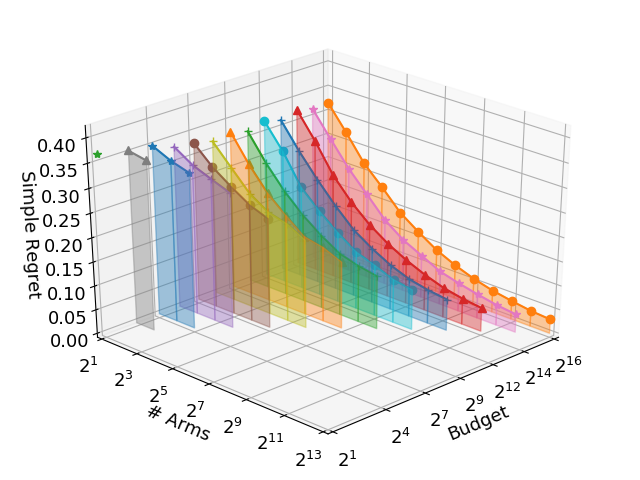
\includegraphics[width=\textwidth]{fixedbudget/figures/folder1/alpha1_beta3_scaled.png}
	\centering
	\caption{$Beta(3,1)$ Scaled.}
	\label{fig:sh-num-arms:alpha1_beta3_scaled}
\end{subfigure}
\begin{subfigure}{0.325\textwidth}%
	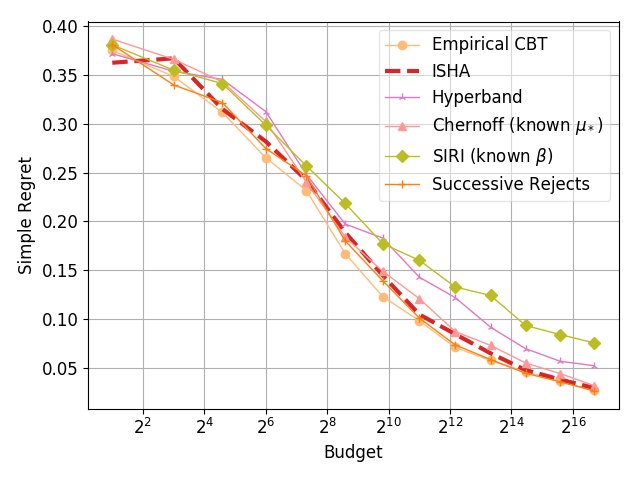
\includegraphics[width=\textwidth]{fixedbudget/figures/folder4/alpha1_beta3_scaled.png}
	\caption{$Beta(3,1)$ Scaled}
	\label{fig:sh-infinite:alpha1_beta3_scaled}
\end{subfigure}
\begin{subfigure}{0.325\textwidth}
	\includegraphics[width=\textwidth]{fixedbudget/figures/folder4/{TwoSpike_0.1_0.515_0.031}.png}
	\caption{Spikes $\pi=10^{-1}, \epsilon=\sqrt{10^{-3}}$}
	\label{fig:sh-infinite:TwoSpike_1}
\end{subfigure}
\begin{subfigure}{0.325\textwidth}%
	\includegraphics[width=\textwidth]{fixedbudget/figures/folder5/alpha1_beta3_scaled.png}
	\caption{$Beta(3,1)$ Scaled}
	\label{fig:sh-lilucb:alpha1_beta3_scaled}
\end{subfigure}
\begin{subfigure}{0.325\textwidth}%
	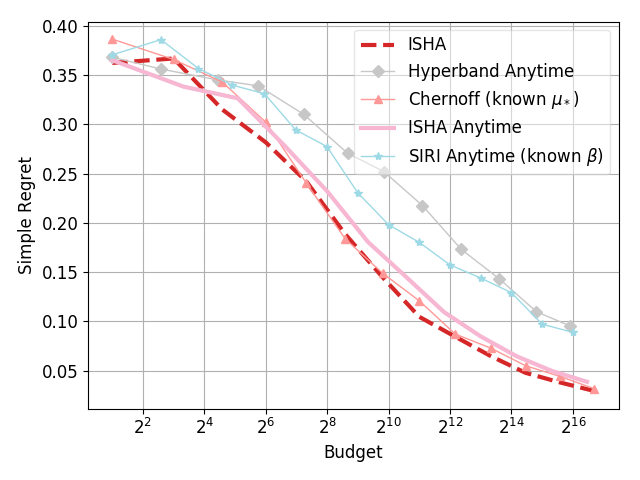
\includegraphics[width=\textwidth]{fixedbudget/figures/folder3/alpha1_beta3_scaled.png}
	\caption{$Beta(3,1)$ Scaled}
	\label{fig:sh-anytime:alpha1_beta3_scaled}
\end{subfigure}
\begin{subfigure}{0.325\textwidth}%
	\includegraphics[width=\textwidth]{fixedbudget/figures/folder2/alpha1_beta1_unscaled.png}
	\caption{$Beta(1,1)$ }
	\label{fig:sh-unscaled-alpha1_beta1_unscaled}
\end{subfigure}
\caption{A sampled set of results. See Section~\ref{appendix:experiments} for more.}
\end{figure}

%\begin{figure}
%\centering
%\caption{Impact of the number of arms for a fixed budget and reservoir.}
%\begin{subfigure}{0.4\textwidth}
%	\includegraphics[width=\textwidth]{figures/folder1/alpha1_beta1_unscaled.png}
%	\caption{$Beta(1,1)$}
%	\label{fig:sh-num-arms:alpha1_beta1_unscaled}
%\end{subfigure}
%\quad
%\begin{subfigure}{0.4\textwidth}
%	\includegraphics[width=\textwidth]{figures/folder1/alpha1_beta1_scaled.png}
%	\caption{$Beta(1,1)$ Scaled}
%	\label{fig:sh-num-arms:alpha1_beta1_scaled}
%\end{subfigure}
%%
%\begin{subfigure}{0.4\textwidth}
%	\includegraphics[width=\textwidth]{figures/folder1/alpha1_beta3_unscaled.png}
%	\caption{$Beta(3,1)$}
%	\label{fig:sh-num-arms:alpha1_beta3_unscaled}
%\end{subfigure}
%\quad
%\begin{subfigure}{0.4\textwidth}
%	\includegraphics[width=\textwidth]{figures/folder1/alpha1_beta3_scaled.png}
%	\caption{$Beta(3,1)$ Scaled}
%	\label{fig:sh-num-arms:alpha1_beta3_scaled}
%\end{subfigure}
%%
%\begin{subfigure}{0.4\textwidth}
%	\includegraphics[width=\textwidth]{figures/folder1/{TwoSpike_0.1_0.515_0.031}.png}
%	\caption{TwoSpike $\alpha=0.1, \epsilon=\sqrt{0.001}$}
%	\label{fig:sh-num-arms:TwoSpike_1}
%\end{subfigure}
%\quad
%\begin{subfigure}{0.4\textwidth}
%	\includegraphics[width=\textwidth]{figures/folder1/{TwoSpike_0.01_0.55_0.1}.png}
%	\caption{Two Spike $\alpha=0.01, \epsilon=\sqrt{0.01}$}
%	\label{fig:sh-num-arms:TwoSpike_2}
%\end{subfigure}
%%
%\begin{subfigure}{0.4\textwidth}
%	\includegraphics[width=\textwidth]{figures/folder1/{TwoSpike_0.001_0.658_0.316}.png}
%	\caption{Two Spike $\alpha=0.001, \epsilon=\sqrt{0.1}$}
%	\label{fig:sh-num-arms:TwoSpike_3}
%\end{subfigure}
%\quad
%\begin{subfigure}{0.4\textwidth}
%	\includegraphics[width=\textwidth]{figures/folder1/new_yorker.png}
%	\caption{New Yorker}
%	\label{fig:sh-num-arms:new_yorker}
%\end{subfigure}
%\label{fig:sh-num-arms}
%\end{figure}
%
%\begin{figure}
%\centering
%\caption{Comparison to state-of-the-art pure exploration infinite bandit algorithms}
%\begin{subfigure}{0.4\textwidth}
%	\includegraphics[width=\textwidth]{figures/folder4/alpha1_beta1_unscaled.png}
%	\caption{$Beta(1,1)$}
%	\label{fig:sh-infinite:alpha1_beta1_unscaled}
%\end{subfigure}
%\quad
%\begin{subfigure}{0.4\textwidth}
%	\includegraphics[width=\textwidth]{figures/folder4/alpha1_beta1_scaled.png}
%	\caption{$Beta(1,1)$ Scaled}
%	\label{fig:sh-infinite:alpha1_beta1_scaled}
%\end{subfigure}
%%
%\begin{subfigure}{0.4\textwidth}
%	\includegraphics[width=\textwidth]{figures/folder4/alpha1_beta3_unscaled.png}
%	\caption{$Beta(3,1)$}
%	\label{fig:sh-infinite:alpha1_beta3_unscaled}
%\end{subfigure}
%\quad
%\begin{subfigure}{0.4\textwidth}
%	\includegraphics[width=\textwidth]{figures/folder4/alpha1_beta3_scaled.png}
%	\caption{$Beta(3,1)$ Scaled}
%	\label{fig:sh-infinite:alpha1_beta3_scaled}
%\end{subfigure}
%%
%\begin{subfigure}{0.4\textwidth}
%	\includegraphics[width=\textwidth]{figures/folder4/{TwoSpike_0.1_0.515_0.031}.png}
%	\caption{TwoSpike $\alpha=0.1, \epsilon=\sqrt{0.001}$}
%	\label{fig:sh-infinite:TwoSpike_1}
%\end{subfigure}
%\quad
%\begin{subfigure}{0.4\textwidth}
%	\includegraphics[width=\textwidth]{figures/folder4/{TwoSpike_0.01_0.55_0.1}.png}
%	\caption{Two Spike $\alpha=0.01, \epsilon=\sqrt{0.01}$}
%	\label{fig:sh-infinite:TwoSpike_2}
%\end{subfigure}
%%
%\begin{subfigure}{0.4\textwidth}
%	\includegraphics[width=\textwidth]{figures/folder4/{TwoSpike_0.001_0.658_0.316}.png}
%	\caption{Two Spike $\alpha=0.001, \epsilon=\sqrt{0.1}$}
%	\label{fig:sh-infinite:TwoSpike_3}
%\end{subfigure}
%\quad
%\begin{subfigure}{0.4\textwidth}
%	\includegraphics[width=\textwidth]{figures/folder4/new_yorker.png}
%	\caption{New Yorker}
%	\label{fig:sh-infinite:new_yorker}
%\end{subfigure}
%\label{fig:sh-infinite}
%\end{figure}
%
%
%\begin{figure}
%\centering
%\caption{Comparison to lil'UCB}
%\begin{subfigure}{0.4\textwidth}
%	\includegraphics[width=\textwidth]{figures/folder5/alpha1_beta1_unscaled.png}
%	\caption{$Beta(1,1)$}
%	\label{fig:sh-lilucb:alpha1_beta1_unscaled}
%\end{subfigure}
%\quad
%\begin{subfigure}{0.4\textwidth}
%	\includegraphics[width=\textwidth]{figures/folder5/alpha1_beta1_scaled.png}
%	\caption{$Beta(1,1)$ Scaled}
%	\label{fig:sh-lilucb:alpha1_beta1_scaled}
%\end{subfigure}
%%
%\begin{subfigure}{0.4\textwidth}
%	\includegraphics[width=\textwidth]{figures/folder5/alpha1_beta3_unscaled.png}
%	\caption{$Beta(3,1)$}
%	\label{fig:sh-lilucb:alpha1_beta3_unscaled}
%\end{subfigure}
%\quad
%\begin{subfigure}{0.4\textwidth}
%	\includegraphics[width=\textwidth]{figures/folder5/alpha1_beta3_scaled.png}
%	\caption{$Beta(3,1)$ Scaled}
%	\label{fig:sh-lilucb:alpha1_beta3_scaled}
%\end{subfigure}
%%
%%\begin{subfigure}{0.4\textwidth}
%%	\includegraphics[width=\textwidth]{figures/folder5/new_yorker.png}
%%	\caption{New Yorker}
%%	\label{fig:sh-lilucb:new_yorker}
%%\end{subfigure}
%\label{fig:sh-lilucb}
%\end{figure}
%
%
%\begin{figure}
%\centering
%\caption{Comparison to state-of-the-art explore-vs-exploit infinite bandit algorithms}
%\begin{subfigure}{0.4\textwidth}
%	\includegraphics[width=\textwidth]{figures/folder2/alpha1_beta1_unscaled.png}
%	\caption{$Beta(1,1)$}
%	\label{fig:sh-unscaled-alpha1_beta1_unscaled}
%\end{subfigure}
%\quad
%\begin{subfigure}{0.4\textwidth}
%	\includegraphics[width=\textwidth]{figures/folder2/alpha1_beta3_unscaled.png}
%	\caption{$Beta(3,1)$}
%	\label{fig:sh-unscaled-alpha1_beta3_unscaled}
%\end{subfigure}
%\label{fig:sh-unscaled}
%\end{figure}
%
%
%\begin{figure}
%\centering
%\caption{Anytime Performance}
%\begin{subfigure}{0.4\textwidth}
%	\includegraphics[width=\textwidth]{figures/folder3/alpha1_beta1_unscaled.png}
%	\caption{$Beta(1,1)$}
%	\label{fig:sh-anytime:alpha1_beta1_unscaled}
%\end{subfigure}
%\quad
%\begin{subfigure}{0.4\textwidth}
%	\includegraphics[width=\textwidth]{figures/folder3/alpha1_beta1_scaled.png}
%	\caption{$Beta(1,1)$ Scaled}
%	\label{fig:sh-anytime:alpha1_beta1_scaled}
%\end{subfigure}
%%
%\begin{subfigure}{0.4\textwidth}
%	\includegraphics[width=\textwidth]{figures/folder3/alpha1_beta3_unscaled.png}
%	\caption{$Beta(3,1)$}
%	\label{fig:sh-anytime:alpha1_beta3_unscaled}
%\end{subfigure}
%\quad
%\begin{subfigure}{0.4\textwidth}
%	\includegraphics[width=\textwidth]{figures/folder3/alpha1_beta3_scaled.png}
%	\caption{$Beta(3,1)$ Scaled}
%	\label{fig:sh-anytime:alpha1_beta3_scaled}
%\end{subfigure}
%%
%\label{fig:sh-anytime}
%\end{figure}

\clearpage
%\clearpage
%\appendix
%!TEX root = main.tex

\subsection{Additional Proofs}\label{sec:appendix_upper_lemmas}
%\subsubsection{Proof of Lemma~\ref{lem:concentration_in_k}}\label{sec:concentration_in_k_proof}
%\begin{lemma}
%Assume Assumption~\ref{asm:subgauss} holds.
%We have
%\begin{align*}
%\P\left( \bigcup_{\ell=0}^{\log_2(n)-1} \bigcup_{i \in S_{\ell}} \left\{ |\widehat{\mu}_{i,\ell} - \mu_i| \geq \Delta_\ell/2 \right\} \right) \leq \delta/2
%\end{align*}
%\end{lemma}
%\begin{proof}
%By Assumption~\ref{asm:subgauss} and a Chernoff bound, recalling that for the $i$th arm $\widehat{\mu}_{i,\ell}$ is empirical mean of $2^\ell$ i.i.d. draws from $\phi(\mu_i)$, we have 
%\begin{align*}
%\P\left( |\widehat{\mu}_{i,\ell} - \mu_i| \geq \Delta_\ell/2 \right) &\leq 2 \exp( -2^{\ell} (\Delta_\ell/2)^2/2 R ) = 2 \frac{\delta}{n \log_2(n) 2^{-\ell+2}} = \frac{\delta /2}{ |S_\ell| \log_2(n)}
%\end{align*}
%By a union bound and conditioning on the elements in $S_\ell$
%\begin{align*}
%\P\left( \bigcup_{\ell=0}^{\log_2(n)-1} \bigcup_{i \in S_{\ell}} \left\{ |\widehat{\mu}_{i,\ell} - \mu_i| \geq \Delta_\ell/2 \right\} \right)  &\leq \sum_{\ell=0}^{\log_2(n)-1} \E\left[ \P\left( \bigcup_{i \in S_{\ell}} \left\{ |\widehat{\mu}_{i,\ell} - \mu_i| \geq \Delta_\ell/2 \right\} \Big| S_\ell \right) \right] \\ 
%&\leq \sum_{\ell=0}^{\log_2(n)-1} \E\left[  \sum_{i \in S_{\ell}} \P\left( |\widehat{\mu}_{i,\ell} - \mu_i| \geq \Delta_\ell/2 \right) \right] \\
%&\leq \sum_{\ell=0}^{\log_2(n)-1} \E\left[  \sum_{i \in S_{\ell}} \frac{\delta /2}{ |S_\ell| \log_2(n)} \right]  \leq \delta/2
%\end{align*}
%
%\end{proof}
%
%\subsubsection{Proof of Lemma~\ref{lem:good_arms_in_set_k}}\label{sec:good_arms_in_set_k_proof}
%\begin{lemma}
%For any $\ell=0,1,\dots,\log_2(n)-1$ if  $n \geq \xi_{n,\ell} := \frac{\log(2 \log_2(n)/\delta)}{2^{-\ell} \nu_\ell(\mu_* + \Delta_\ell)}$ then 
%% If $n \geq \max_{\ell =0,1,\dots, \log_2(n)-1} \frac{\log(2 \log_2(n)/\delta)}{2^{-\ell} \nu_\ell(\mu_* + \Delta_\ell)}$ then
%\begin{align*}
%\P\left(\min_{i \in S_\ell} \mu_i > \mu_* + \Delta_\ell \right) \leq \tfrac{\delta}{2 \log_2(n)}.
%\end{align*}
%Moreover, $\P\left( \bigcup_{\ell=0}^{\log_2(n)-1} \left\{ \min_{i \in S_\ell} \mu_i > \mu_* + \Delta_\ell \right\} \right)\leq\delta/2$ whenever $n \geq \max_{\ell=0,1,\dots,\log_2(n)-1} \xi_{n,\ell}$.
%\end{lemma}
%\begin{proof}
%By a union bound we have
%\begin{align*}
%\P\left( \bigcup_{\ell=0}^{\log_2(n)-1} \left\{ \min_{i \in S_\ell} \mu_i > \mu_* + \Delta_\ell \right\} \right) 
%&\leq  \sum_{\ell=0}^{\log_2(n)-1} \P(\min_{i \in S_\ell} \mu_i > \mu_* + \Delta_\ell)
%\end{align*}
%so it suffices to show
%\begin{align*}
%\P(\min_{i \in S_\ell} \mu_i > \mu_* + \Delta_\ell) &=
%\E\left[ \P\left( \min_{i \in S_\ell} \mu_i > \mu_* + \Delta_\ell \Big| S_\ell \right) \right] \\
%&=  \P\left( \min_{i =1,\dots, |S_\ell|} \mu_i > \mu_* + \Delta_\ell \Big| \{\mu_i \}_{i=1}^{|S_\ell|} \overset{iid}{\sim} \nu_\ell \right)  \\
%&=  \P\left( \mu_i > \mu_* + \Delta_\ell \Big| \mu_i \overset{iid}{\sim} \nu_\ell \right)^{|S_\ell|} \\
%&=  \left( 1- \nu_\ell( \mu_* + \Delta_\ell) \right)^{|S_\ell|}  \\
%&\leq  \exp\left( - n 2^{-\ell}\nu_\ell( \mu_* + \Delta_\ell) \right) \\
%&\leq  \frac{\delta}{2\log_2(n)}
%\end{align*}
%where the second-to-last line uses the identity $n 2^{-\ell} = |S_\ell|$ and that $1-x \leq e^{-x}$ for all $x\geq0$, and the last line plugs in the assumed condition on $n$.
%\end{proof}
%
%\subsubsection{Proof of Lemma~\ref{lem:core_lemma}} \label{sec:core_lemma_proof}
%\begin{lemma}
%Assume Assumption~\ref{asm:stochastic_ordering} holds.
%For any $k$ and $x\in \R$ we have
%\begin{align*}
%\nu_{k+1}(x) &= 2 \P( \mu_i \in S_{k+1} \, | \, \mu_i \leq x, \mu_i \in S_{k} ) \, \nu_k(x)\\
%&\geq \nu_k(x).
%\end{align*}
%Moreover, for any $k$ and $x < y$ we have $\frac{\nu_{k+1}(x)}{\nu_k(x)} \geq \frac{\nu_{k+1}(y)}{\nu_k(y)}$.
%% \begin{align*}
%% \frac{\nu_{k+1}(x)}{\nu_k(x)} \geq \frac{\nu_{k+1}(y)}{\nu_k(y)}.
%% \end{align*}
%\end{lemma} 
%\begin{proof}
%By Bayes' rule
%\begin{align*}
%\nu_{k+1}(x) &= \P( \mu_i \leq x \, | \, \mu_i \in S_{k+1} )\\
%&= \P( \mu_i \leq x \, | \, \mu_i \in S_{k+1}, \mu_i \in S_{k} )\\
%&= \frac{ \P( \mu_i \in S_{k+1} \, | \, \mu_i \leq x, \mu_i \in S_{k} ) \P( \mu_i \leq x \, | \, \mu_i \in S_{k}) }{ \P(\mu_i \in S_{k+1} \, | \, \mu_i \in S_{k}) }  \\
%&= \nu_k(x) \frac{\P( \mu_i \in S_{k+1} \, | \, \mu_i \leq x, \mu_i \in S_{k} )}{\P(\mu_i \in S_{k+1} \, | \, \mu_i \in S_{k})}.
%\end{align*}
%By definition, $\P(\mu_i \in S_{k+1} \, | \, \mu_i \in S_{k}) = \frac{1}{2}$. 
%On the other hand, ignoring ties (which are broken randomly) we have $\mu_i \in S_{k+1} \iff \widehat{\mu}_{i,k} \leq \tau$.
%Thus, by assumption 1,
%\begin{align*}
%\P( \mu_i \in S_{k+1} \, | \, \mu_i > x, \mu_i \in S_{k} ) \leq \P( \mu_i \in S_{k+1} \, | \, \mu_i \leq x, \mu_i \in S_{k} ).
%\end{align*}
%Applying the law of total probability to $\P(\mu_i \in S_{k+1} \, | \, \mu_i \in S_{k})$ we have
%\begin{align*}
%\hspace{1in}&\hspace{-1in}\frac{\P( \mu_i \in S_{k+1} \, | \, \mu_i \leq x, \mu_i \in S_{k} )}{\P(\mu_i \in S_{k+1} \, | \, \mu_i \in S_{k})}\\
%&= \frac{\P( \mu_i \in S_{k+1} \, | \, \mu_i \leq x, \mu_i \in S_{k} )}{ \nu_k(x) \P( \mu_i \in S_{k+1} \, | \, \mu_i \leq x, \mu_i \in S_{k} ) + (1-\nu_k(x)) \P( \mu_i \in S_{k+1} \, | \, \mu_i > x, \mu_i \in S_{k} )}\\
%&\geq \frac{\P( \mu_i \in S_{k+1} \, | \, \mu_i \leq x, \mu_i \in S_{k} )}{ \nu_k(x) \P( \mu_i \in S_{k+1} \, | \, \mu_i \leq x, \mu_i \in S_{k} ) + (1-\nu_k(x)) \P( \mu_i \in S_{k+1} \, | \, \mu_i \leq x, \mu_i \in S_{k} )} \\
%&= 1.
%\end{align*}
%To obtain the final result, note that
%\begin{align*}
%\frac{\nu_{k+1}(x)}{\nu_k(x)} &= \frac{\P( \mu_i \in S_{k+1} \, | \, \mu_i \leq x, \mu_i \in S_{k} )}{\P(\mu_i \in S_{k+1} \, | \, \mu_i \in S_{k})} \\
%&\geq \frac{\P( \mu_i \in S_{k+1} \, | \, \mu_i \leq y, \mu_i \in S_{k} )}{\P(\mu_i \in S_{k+1} \, | \, \mu_i \in S_{k})} = \frac{\nu_{k+1}(y)}{\nu_k(y)}
%\end{align*}
%\end{proof}

\subsubsection{Proof of Lemma~\ref{lem:exp_N1}}

\begin{proof}
By a manipulation of Wald's identity \cite{WaldsLemma}, if $N$ is a stopping time with finite expectation at which time the procedure declares the arm as $\epsilon$-good or not when run on an arm with mean $\mu$, we have for any $\mu' \neq \mu$
\begin{align}
\E_\mu[N] \geq \frac{\sup_{\mathcal{E}} d( \P_\mu(\mathcal{E}), \P_{\mu'}(\mathcal{E}) )}{KL(\mu,\mu')} \label{eqn:wald}
\end{align}
where $d(x,y) = x \log(\frac{x}{y}) + (1-x) \log(\frac{1-x}{1-y})$.
Now
\begin{align*}
\int_{\mu=\mu_*} \E_\mu[N] d\nu(\mu) &= \int_{\mu=\mu_*}^{\mu_*+\epsilon} \E_\mu[N] d\nu(\mu) + \int_{\mu=\mu_*+\epsilon}^\infty \E_\mu[N] d\nu(\mu) .
\end{align*}


Consider the decomposition $\nu = \nu^a + \nu^s$ where $\nu^a$ and $\nu^s$ are the absolutely continuous and singular components, respectively, of $\nu$ with respect to the Lebesgue measure.
Let $\A^\circ = \{ \{a\} : a \in [\mu_* + \epsilon,\infty) \cap \mathrm{support}(\nu^s),  \frac{d\nu^s(a)}{dx} \geq \kappa \}$ where $\frac{d\nu^s(a)}{dx}$ is the Radon-Nikodym derivative with respect to the Lebesgue measure.
Note that $\A^\circ$ does not contain \emph{all} of the singular components, just those with mass at least $\kappa$.
Let $\A^\perp$ be a collection of disjoint sets that have empty intersection with $\A^\circ$ 
constructed by first covering $[\mu_* + \epsilon,\infty) \cap \mathrm{support}(\nu)-\A^\circ$ with intervals such that $A$ is an interval, $\kappa \leq \nu(A-\A^\circ) \leq 2 \kappa$, and then set $A \leftarrow A \setminus \A^\circ$ such that $A$ is an interval in all but a set of measure $0$.
Finally, define $\A = \A^\circ \cup \A^\perp$.
Note that $\min_{A \in \A} \nu(A) \geq \kappa$.
Also note that for any $A \in \A$ we have $\sup_{x,y \in A} |x-y| > 0$ if and only if $A \in \A^\perp$ so that we also have $\nu(A) \leq 2 \kappa$.  


% Fix $\kappa \in (0,1)$. 
% Let $t_0 = \mu_* + \epsilon$ and let $\A =\{A_1,A_2,\dots\}$ where $A_k = (t_{k-1}, t_k]$ and $t_k = \min\{ t : \nu(t) \geq \nu(t_{k-1}) + \kappa\}$ so that $\nu(A_k) \geq \kappa$ and $A_{k+1} = \arg\sup_{A \subset \R \setminus \{A_{\ell}\}_{\ell < k}: \nu(A)\geq \kappa} \frac{\nu(A)}{\sup_{x \in A} KL(\mu_*, x)}$
% Inflate the last set so that so that it contains the support. 

Let $E$ denote the event that the current arm is the declared as $\epsilon$-good.
Given such a partition, note that
\begin{align*}
\max_{A \in \A} \frac{1}{\nu(A)} \int_{\mu \in A} \P_\mu(E) d\nu(\mu) &\leq \sum_{A \in \A} \frac{1}{\nu(A)} \int_{\mu \in A} \P_\mu(E) d\nu(\mu) \\
&\leq \frac{1}{\kappa} \sum_{A \in \A} \int_{\mu \in A} \P_\mu(E) d\nu(\mu) \\
&= \frac{1}{\kappa} \int_{\mu = \mu_* + \epsilon} \P_\mu(E) d\nu(\mu) \\
&=  \frac{\alpha(1-\pi)}{\kappa}  \\
&< 1-\beta
\end{align*}
where the last line holds by assumption.
By the definition of $\widetilde{\mu}$ in the statement, if $\widetilde{A} = (\mu_*+\epsilon, \widetilde{\mu}]$ then $\nu(\widetilde{A}) \geq \kappa$ so
\begin{align*}
\int_{\mu=\mu_*}^{\mu_*+\epsilon} \E_\mu[N] d\nu(\mu) &= \pi \frac{1}{\nu(\widetilde{A})}  \int_{\mu' \in \widetilde{A}} \frac{1}{\pi} \int_{\mu=\mu_*}^{\mu_*+\epsilon} \E_\mu[N] d\nu(\mu) d\nu(\mu')\\
&\overset{(i)}{\geq} \pi  \frac{1}{\nu(\widetilde{A})} \int_{\mu' \in \widetilde{A}} \frac{1}{\pi} \int_{\mu=\mu_*}^{\mu_*+\epsilon} \frac{d( \P_\mu(E), \P_{\mu'}(E) )}{KL(\mu,\mu')}  d\nu(\mu) d\nu(\mu') \\
&\overset{(ii)}{\geq} \pi  \frac{1}{KL(\mu_*,\widetilde{\mu})} \frac{1}{\nu(\widetilde{A})} \int_{\mu' \in \widetilde{A}} \frac{1}{\pi} \int_{\mu=\mu_*}^{\mu_*+\epsilon} d( \P_\mu(E), \P_{\mu'}(E) )  d\nu(\mu) d\nu(\mu') \\
&\overset{(iii)}{\geq}  \pi  \frac{1}{KL(\mu_*,\widetilde{\mu})} d\left( \frac{1}{\pi} \int_{\mu=\mu_*}^{\mu_*+\epsilon} \P_\mu(E)d\nu(\mu) , \frac{1}{\nu(\widetilde{A})} \int_{\mu' \in \widetilde{A}}  \P_{\mu'}(E) d\nu(\mu') \right)    \\
&\overset{(iv)}{\geq} \pi  d(1-\beta,  \tfrac{\alpha(1-\pi)}{\nu(\widetilde{A})}) \frac{1}{KL(\mu_*,\widetilde{\mu})} 
\end{align*}
where $(i)$ follows from Equation~\ref{eqn:wald}, 
$(ii)$ uses the fact that $KL(a,b) \leq KL(c,d)$ whenever $[a,b] \subseteq [c,d]$, 
$(iii)$ uses the fact that binary KL divergence is convex \cite{Cover:2006:EIT:1146355}, 
and $(iv)$ holds because $\max_{A \in \A} \frac{1}{\nu(A)}\int_{\mu \in A} \P_\mu(E) d\nu(\mu) \leq \frac{\alpha(1-\pi)}{\kappa} < 1-\beta$ by assumption.


The second term follows analogously
\begin{align*}
\int_{\mu=\mu_*+\epsilon}^\infty \E_\mu[N] d\nu(\mu) &= \sum_{A \in \A} \nu(A) \frac{1}{\nu(A)} \int_{\mu \in A} \E_\mu[N] d\nu(\mu) \\
&= \sum_{A \in \A} \nu(A) \frac{1}{\pi}\int_{\mu' =\mu_*}^{\mu_* + \epsilon} \frac{1}{\nu(A)} \int_{\mu \in A} \E_\mu[N] d\nu(\mu) d\nu(\mu')\\
&\overset{(i)}{\geq} \sum_{A \in \A} \nu(A)\frac{1}{\pi}\int_{\mu' =\mu_*}^{\mu_* + \epsilon} \frac{1}{\nu(A)} \int_{\mu \in A} \frac{d( \P_\mu(E), \P_{\mu'}(E) )}{KL(\mu,\mu')}  d\nu(\mu) d\nu(\mu') \\
&\overset{(ii)}{\geq} \sum_{A \in \A}  \frac{\nu(A)}{\sup_{\mu \in A} KL(\mu,\mu_*)} \frac{1}{\pi}\int_{\mu' =\mu_*}^{\mu_* + \epsilon}\frac{1}{\nu(A)} \int_{\mu \in A} d( \P_\mu(E), \P_{\mu'}(E) )  d\nu(\mu) d\nu(\mu') \\
&\overset{(iii)}{\geq} \sum_{A \in \A} \frac{\nu(A)}{\sup_{\mu \in A} KL(\mu,\mu_*)} d\left( \frac{1}{\nu(A)}\int_{\mu \in A}  \P_\mu(E) d\nu(\mu) , \frac{1}{\pi}\int_{\mu' =\mu_*}^{\mu_* + \epsilon} \P_{\mu'}(E) d\nu(\mu')\right)  \\
&\overset{(iv)}{\geq} d\left( \tfrac{\alpha(1-\pi)}{\kappa} , 1-\beta \right) \sum_{A \in \A}  \frac{\nu(A)}{\sup_{\mu \in A} KL(\mu,\mu_*)}  
\end{align*}
where $(i)-(iv)$ follow for identical reasons as above.

Index the sets of $\A^\perp$ into $A_1,A_2,\dots,A_{|\A^\perp|}$ where $\sup_{x \in A_k} x \leq \inf_{y \in A_{k+1}} y$ for all $k$. 
Recalling that $\sup_{x \in A} x = \inf_{x \in A} x$ for all $A \in \A^\circ$ and $\kappa \leq \nu(A) \leq 2\kappa$ for all $A \in \A^\perp$ we have 
\begin{align*}
\sum_{A \in \A}  \frac{\nu(A)}{\sup_{\mu \in A} KL(\mu,\mu_*)} 
&= \sum_{k = 1}^{|\A^\perp|}  \frac{\nu(A_k)}{\sup_{\mu \in A_k} KL(\mu,\mu_*)} + \sum_{A \in \A^\circ}  \frac{\nu(A)}{\inf_{\mu \in A} KL(\mu,\mu_*)} \\
&\geq \sum_{k = 1}^{|\A^\perp|-1}  \frac{\nu(A_{k+1})/2}{\sup_{\mu \in A_k} KL(\mu,\mu_*)} + \sum_{A \in \A^\circ}  \frac{\nu(A)}{\inf_{\mu \in A} KL(\mu,\mu_*)} \\
&\geq \sum_{k = 1}^{|\A^\perp|-1}  \frac{\nu(A_{k+1})/2}{\inf_{\mu \in A_{k+1}} KL(\mu,\mu_*)} + \sum_{A \in \A^\circ}  \frac{\nu(A)}{\inf_{\mu \in A} KL(\mu,\mu_*)} \\
% &=  \frac{\nu(A_1)}{\sup_{\mu \in A_1} KL(\mu,\mu_*)} + \sum_{A_k \in \A^\perp \setminus A_{1}}  \frac{\nu(A_{k})}{\sup_{\mu \in A_{k}} KL(\mu,\mu_*)} + \sum_{A \in \A^\circ}  \frac{\nu(A)}{\inf_{\mu \in A} KL(\mu,\mu_*)} \\
% &\geq  \frac{\nu(A_2)/2}{\sup_{\mu \in A_1} KL(\mu,\mu_*)} + \sum_{A_k \in \A^\perp \setminus A_{1}}  \frac{\nu(A_{k})}{\sup_{\mu \in A_{k}} KL(\mu,\mu_*)} + \sum_{A \in \A^\circ}  \frac{\nu(A)}{\inf_{\mu \in A} KL(\mu,\mu_*)} \\
% &\geq  \frac{\nu(A_2)/2}{\inf_{\mu \in A_2} KL(\mu,\mu_*)} + \sum_{A_k \in \A^\perp \setminus A_{1}}  \frac{\nu(A_{k})}{\sup_{\mu \in A_{k}} KL(\mu,\mu_*)} + \sum_{A \in \A^\circ}  \frac{\nu(A)}{\inf_{\mu \in A} KL(\mu,\mu_*)} \\
&=   \sum_{k = 2}^{|\A^\perp|}  \frac{\nu(A_k)/2}{\inf_{\mu \in A_k} KL(\mu,\mu_*)} + \sum_{A \in \A^\circ}  \frac{\nu(A)}{\inf_{\mu \in A} KL(\mu,\mu_*)}\\
&=  -\frac{\nu(A_1)/2}{\inf_{\mu \in A_1} KL(\mu,\mu_*)} + \sum_{A \in \A}  \frac{\nu(A)/2}{\inf_{\mu \in A} KL(\mu,\mu_*)}\\
&\geq   -\frac{\kappa}{KL(\mu_*+\epsilon,\mu_*)}  + \frac{1}{2} \int_{\mu_*+\epsilon} \frac{1}{KL(\mu,\mu_*)} d\nu(\mu) 
 \end{align*}
 % We immediately have $\frac{\nu(A_1)/2}{\inf_{\mu \in A_1} KL(\mu,\mu_*)} \leq \frac{\kappa}{KL(\mu_*+\epsilon,\mu_*)}$.
 % However, we can get a tighter representation by considering the definition of $A_1$.
% While $A_1$ may contain a singular component we also know $\nu^s(A_1) + \nu^a(A_1) \leq 2\kappa$ so we clearly have $\sup\{\mu:\mu \in A_1\} \leq \dot{\mu}$ where $\dot{\mu} = \sup\{ \mu : \nu^a(\mu) - \nu^a(\mu_*+\epsilon) \leq 2\kappa \}$
%  so that
%  \begin{align*}
%  -\frac{\nu(A_1)/2}{\inf_{\mu \in A_1} KL(\mu,\mu_*)}  + \frac{1}{2} \int_{\mu_*+\epsilon} \frac{1}{KL(\mu,\mu_*)} d\nu(\mu) \geq \frac{1}{2} \int_{\dot{\mu}} \frac{1}{KL(\mu,\mu_*)} d\nu(\mu)
%  \end{align*}
%  Trivially we have
%  \begin{align*}
%  \int_{\dot{\mu}} \frac{1}{KL(\mu,\mu_*)} d\nu(\mu) \geq \frac{-2\kappa}{KL(\mu_*+\epsilon,\mu_*)} + \int_{\mu_*+\epsilon} \frac{1}{KL(\mu,\mu_*)} d\nu(\mu)
%  \end{align*}
so that
 \begin{align*}
 \int_{\mu=\mu_*+\epsilon}^\infty \E_\mu[N] d\nu(\mu) \geq d\left( \tfrac{\alpha(1-\pi)}{\kappa}, 1-\beta \right) \left(  - \frac{\kappa}{KL(\mu_* + \epsilon, \mu_*)}  + \frac{1}{2} \int_{\mu_*+\epsilon} \frac{1}{KL(\mu,\mu_*)} d\nu(\mu) \right).
 \end{align*}
 \end{proof}

\subsubsection{Proof of Theorem~\ref{thm:fb-lb}}

\begin{proof}
We plug in the result of Lemma~\ref{lem:exp_N1} with $\kappa=2\pi$ into Equation~\ref{eqn:N1_to_many} to obtain
\begin{align*}
\E[ \sum_{i \geq 1} N_i ] \geq& \pi \frac{ d\left(1-\beta,  \tfrac{\alpha(1-\pi)}{\widetilde{\kappa}}\right) }{\alpha (1-\pi) + (1-\beta) \pi} \frac{1}{KL(\mu_*,\widetilde{\mu})}  \\
&+\frac{
d\left(\tfrac{\alpha(1-\pi)}{\kappa} , 1-\beta \right)}{\alpha (1-\pi) + (1-\beta) \pi} \left(  - \frac{\kappa}{KL(\mu_* + \epsilon, \mu_*)}  + \frac{1}{2} \int_{\mu_*+\epsilon} \frac{1}{KL(\mu,\mu_*)} d\nu(\mu) \right).
\end{align*}

For the first term we apply the assumption $\frac{(1-\pi)\alpha}{\pi(1-\beta)} \leq \frac{\delta}{1-\delta}$  to obtain
\begin{align*}
\frac{\pi \, d(1-\beta,  \tfrac{\alpha(1-\pi)}{\widetilde{\kappa}})}{\alpha (1-\pi) + (1-\beta) \pi} &\geq \frac{d(1-\beta, \tfrac{\delta \pi}{(1-\delta)\widetilde{\kappa}} (1-\beta))}{(1-\beta) /(1-\delta)} \\
&= \frac{(1-\beta) \log(\tfrac{(1-\delta)\widetilde{\kappa}}{\delta \pi}) + \beta \log(\beta)  - \beta \log(1-\tfrac{\delta \pi (1-\beta)}{(1-\delta)\kappa})}{(1-\beta) /(1-\delta)} \\
&\geq (1-\delta) \log(\tfrac{(1-\delta)\widetilde{\kappa}}{\delta \pi}) + (1-\delta) \tfrac{\beta}{1-\beta} \log(\beta) \\
&\geq (1-\delta) \log(\tfrac{(1-\delta)\widetilde{\kappa}}{\delta e}) 
\end{align*}
using the fact that $-\tfrac{\beta}{1-\beta} \log(\beta) \in (0,1)$ for $\beta \in (0,1)$.

For the second term we apply the assumption again to get
\begin{align*}
\frac{d\left(\tfrac{\alpha(1-\pi)}{\kappa} , 1-\beta \right)}{\alpha (1-\pi) + (1-\beta) \pi} &\geq \frac{d\left(\tfrac{\pi \delta}{\kappa (1-\delta)} (1-\beta) , 1-\beta \right)}{(1-\beta) \pi/(1-\delta)} \\
&= \frac{ \tfrac{\pi \delta}{\kappa (1-\delta)} (1-\beta) \log(\tfrac{\pi \delta}{\kappa (1-\delta)}) + \left(1- \tfrac{\pi \delta}{\kappa (1-\delta)} (1-\beta)\right) \log( \frac{1- \tfrac{\pi \delta}{\kappa (1-\delta)} (1-\beta)}{\beta})}{(1-\beta) \pi/(1-\delta)} \\
&= \tfrac{1-\delta}{\pi} \tfrac{\pi \delta}{\kappa (1-\delta)}  \log(\tfrac{\pi \delta}{\kappa (1-\delta)}) + \tfrac{1-\delta}{\pi}\left(1- \tfrac{\pi \delta}{\kappa (1-\delta)} (1-\beta)\right)\left( \tfrac{\log(1/\beta)}{1-\beta} + \tfrac{\log\left( 1- \tfrac{\pi \delta}{\kappa (1-\delta)} (1-\beta) \right)}{1-\beta} \right)\\
&\geq \tfrac{1-\delta}{\pi} \tfrac{\delta/2}{1-\delta}  \log(\tfrac{\delta/2}{1-\delta}) + \tfrac{1-\delta}{\pi}\left(1- \tfrac{\delta /2}{ 1-\delta} (1-\beta)\right)\left( 1- \tfrac{\delta}{1-\delta}   \right) \\
&\geq \tfrac{1-\delta}{\pi}( 1 + \tfrac{\delta/2}{1-\delta}  \log(\tfrac{\delta/2}{1-\delta}) - \tfrac{3\delta/2}{1-\delta} ) \\
&\geq \tfrac{1 - \tfrac{\delta}{2}  \log(\tfrac{1-\delta}{\delta/42})}{\pi} 
\end{align*}
where the last lines use $\kappa = 2\pi$, $\tfrac{\log(1/\beta)}{1-\beta} \geq 1$ for all $\beta \in (0,1)$, $\log(1-x) \geq -2x$ for $x \in (0,1/2)$, and $\delta \in (0, 12]$.
Thus, putting the pieces together we obtain
\begin{align*}
\E[ \sum_{i \geq 1} N_i ] &\geq \frac{(1-\delta) \log(\tfrac{(1-\delta)\widetilde{\kappa}}{\delta \pi e})}{KL(\mu_* , \widetilde{\mu})} + \tfrac{1 - \tfrac{\delta}{2}  \log(\tfrac{1-\delta}{\delta/42})}{\pi} \left(  - \frac{ \kappa}{KL(\mu_* + \epsilon, \mu_*)}  + \frac{1}{2} \int_{\mu_*+\epsilon} \frac{1}{KL(\mu,\mu_*)} d\nu(\mu) \right) \\
&= \frac{ (1-\delta) \log(\tfrac{(1-\delta)\widetilde{\kappa}}{\delta \pi e})}{KL(\mu_* , \widetilde{\mu})}  + (1 - \tfrac{\delta}{2}  \log(\tfrac{1-\delta}{\delta/42})) \left(  - \frac{2}{KL(\mu_* + \epsilon, \mu_*)}  + \frac{1}{2\pi} \int_{\mu_*+\epsilon} \frac{1}{KL(\mu,\mu_*)} d\nu(\mu) \right).
\end{align*}
Finally, $1 \geq (1 - \tfrac{\delta}{2}  \log(\tfrac{1-\delta}{\delta/42}))\geq 3/4$ for $\delta \leq 1/15$.

\end{proof}

\subsection {Empirical study}\label{appendix:experiments}

Here we present further results in addition to what we provided in Section~\ref{experiments}. We start with describing in some detail the baselines we used and then present further experiments on various reservoirs.

\textbf{Pure exploration algorithms.}
Our first batch of baselines are pure exploration algorithms.

We introduce the algorithm we call Chernoff, meant as a strong baseline
for ISHA. This algorithm has knowledge of $\mu_*$.
We define the algorithm in terms of the confidence lower bound $L_i(t) = \min \{q \in [0,\widehat{\mu}_{i}] : N_i(t) KL(\hat{\mu}_i(t),q) \le \log(1/\delta_k) \}\label{kl-ub}$
where $t$ is the budget used so far,
$N_i(t)$ is the number of times arm $i$ is pulled,
and $\delta_k = \frac{6\delta}{(\pi N_i(t))^2}$ for $\delta=0.1$ so that the overall error tolerance for an arm $i$ is $\delta$.
This algorithm draws an arm from the reservoir and continues drawing
rewards from it until $L_i(t) > \mu_*$. Once its confidence interval no longer contains $\mu_*$, the arm is discarded and a new arm is drawn.
At time $T$ the algorithm stops and returns the arm that was sampled the most. 

SIRI \citep{DBLP:journals/corr/CarpentierV15} is a recent UCB-style pure exploration algorithm in the fixed budget setting.
It is based on a $\beta$-regularity assumption for the tail of the
reservoir, and so makes use of additional information about the reservoir.
We run this with $\delta=0.1$.

lil'UCB \citep{Jamieson2014lilU}, another UCB algorithm, is a fixed confidence pure exploration algorithm for finite bandits. While the original lil'UCB has its own stopping criterion, in our experiments it stops when it runs out of budget. For consistency, we use the $L_i(t)$ defined for Chernoff with the same $\delta$ value and schedule used therein.

We also run Hyperband~\citep{li2017hyperband}, described earlier.
Its parameter $\eta$ decides which fraction of arms to discard in a given round of Successive Halving. We used $\eta=2$ (discarding half the arms) in keeping with Successive Halving.

Successive Rejects \citep{DBLP:conf/colt/AudibertBM10}, a fixed budget algorithm originally intended for finite bandits, is similar to Successive Halving. We run it with $n^*_T$ arms. 

\paragraph{Explore-vs-Exploit algorithms.}
We use regret minimization infinite bandit algorithms
as our next batch of baselines.
Note that these algorithms are not natural competitors and do not have an arm recommendation strategy. At time $T$ we stop and return the arm that was sampled the most.

We  experiment with four infinite bandit algorithms of \cite{berry1997} designed for $Beta(1,1)$ with support on $[0,1]$:
$f$-failure strategy (with $f=1$) which samples an arm until
$f$ failures are observed,
$s$-run strategy (with $s=\sqrt{T}$) which samples each arm
at most $s$ times until a failure is observed and then exploits the most
successful arm until the budget is exhausted,
$s$-run strategy (non-recall; $s=\sqrt{T}$) which samples from
an arm until the first failure but exploits the arm until the budget
is exhausted if $s$ successes are observed, and
$m$-learning strategy (with $m=\log(T)\sqrt{T}$) which plays the $f$-failure strategy (with $f=1$) for the first $m$
times (the arm at time $m$ is exploited until a failure is observed). From there the empirically-best arm is exploited. 

CBT and Empirical CBT  
\cite{Chan2018Infinite} are also used as baselines.
CBT takes as input a target mean parameter $\mu_{target}=\sqrt{2/T}$ for reservoir $Beta(1,1)$, and $\mu_{target}=\sqrt[4]{4/T}$ for $Beta(3,1)$  and thus assumes
knowledge of the reservoir.
Empirical CBT does not assume anything about the reservoir but
instead estimates $\mu_{target}$. 

Two Target (fixed horizon) \cite{bonald2013two} uses
two success target thresholds
$l_1$ and $l_2$ as function of the reservoir parameters $\beta$ and $\alpha$, and budget $T$.
Any arm which fails to have $l_1$ 
successes before its first failure is discarded,
and any arm which has $l_2$ successes before its first $m$ failures
is subsequently exploited until the budget is exhausted.
We use $m=3$ in our experiments.  


\paragraph{Anytime algorithms.}
We also propose the following Anytime version
of ISHA and compare it to other anytime algorithms.
When an effectively unlimited budget is available, ISHA
Anytime can be run as follows.
Choose increasing dyadic numbers of arms, $n=2^i, i=1,2,\dots$.
For each value of $n$, sample $n$ new arms and
run ISHA and save the result
as the best arm found so far.
We compare this algorithm to Hyperband Anytime and SIRI Anytime (using the budget doubling trick as proposed by the SIRI authors).

\subsubsection{Experiments and Insights}\label{appendix:fb-experiments}
\paragraph{Successive Halving performance as a function of the number of arms for a fixed budget.}
The class of experiments in Figure~\ref{appendix:fig:sh-num-arms} reports the average simple regret for ISHA (Successive Halving using the maximum number of arms s.t. $T \ge n^*_T\log_2 n^*_T$) in comparison to various
smaller choices of $n$. Across a variety of reservoirs, $n^*_T$ arms is always a good choice for Successive Halving in the infinite setting.

\paragraph{Simple regret vs. Budget.} 
In the class of experiments in Figure~\ref{appendix:fig:sh-infinite} we compare the simple regret of
ISHA to that of various pure exploration baselines.
 
Figure~\ref{appendix:fig:sh-lilucb} highlights the difficulty of
choosing the optimal number of arms for UCB-style algorithms,
such as the lil'UCB.

Figure~\ref{appendix:fig:sh-unscaled} compares mainly against various exploration-vs-exploitation baselines, some of which were specifically designed specifically for $Beta$ reservoirs.

Finally, in Figure~\ref{appendix:fig:sh-anytime}, we compare ISHA  and ISHA Anytime to several other anytime algorithms.

\clearpage

\begin{figure}
\centering
\caption{Impact of the number of arms for a fixed budget and reservoir.}
\begin{subfigure}{0.4\textwidth}
	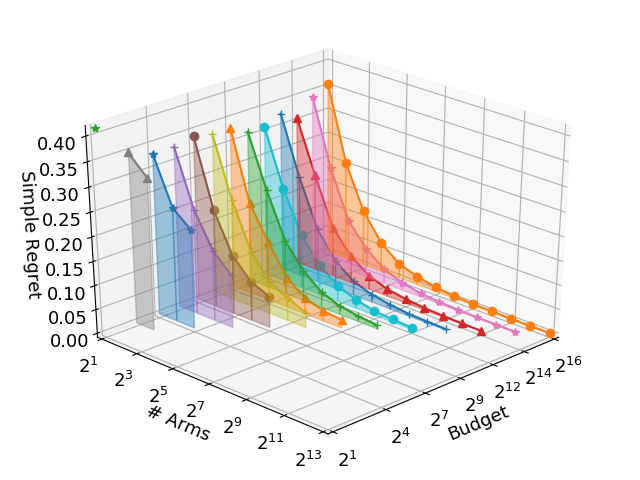
\includegraphics[width=\textwidth]{fixedbudget/figures/folder1/alpha1_beta1_unscaled.png}
	\caption{$Beta(1,1)$}
	\label{appendix:fig:sh-num-arms:alpha1_beta1_unscaled}
\end{subfigure}
\quad
\begin{subfigure}{0.4\textwidth}
	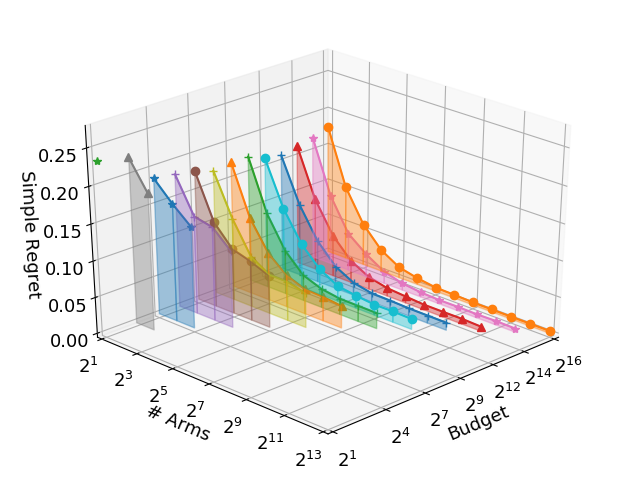
\includegraphics[width=\textwidth]{fixedbudget/figures/folder1/alpha1_beta1_scaled.png}
	\caption{$Beta(1,1)$ Scaled}
	\label{appendix:fig:sh-num-arms:alpha1_beta1_scaled}
\end{subfigure}
%
\begin{subfigure}{0.4\textwidth}
	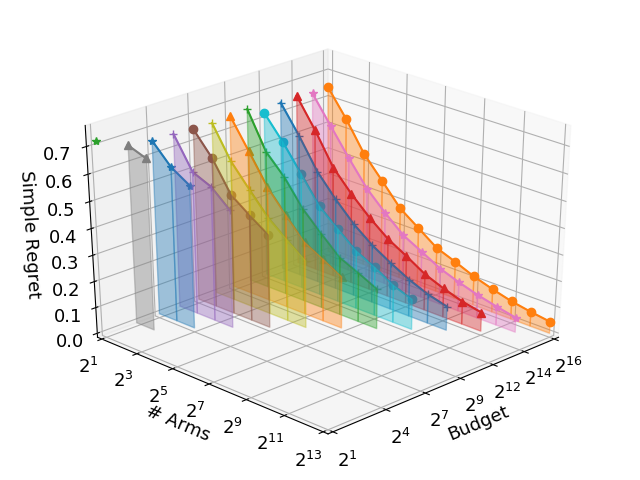
\includegraphics[width=\textwidth]{fixedbudget/figures/folder1/alpha1_beta3_unscaled.png}
	\caption{$Beta(3,1)$}
	\label{appendix:fig:sh-num-arms:alpha1_beta3_unscaled}
\end{subfigure}
\quad
\begin{subfigure}{0.4\textwidth}
	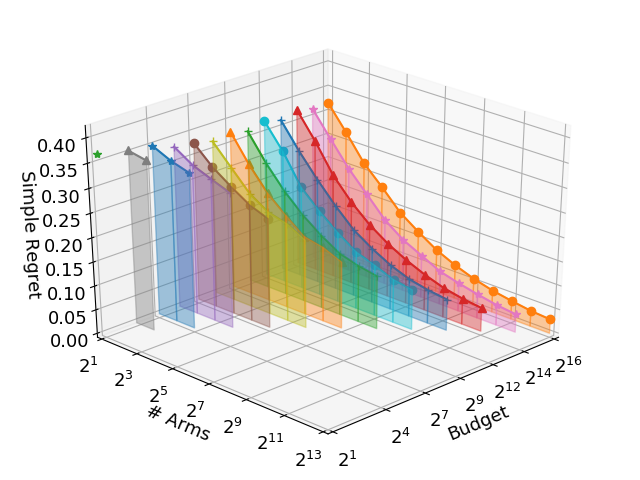
\includegraphics[width=\textwidth]{fixedbudget/figures/folder1/alpha1_beta3_scaled.png}
	\caption{$Beta(3,1)$ Scaled}
	\label{appendix:fig:sh-num-arms:alpha1_beta3_scaled}
\end{subfigure}
%
\begin{subfigure}{0.4\textwidth}
	\includegraphics[width=\textwidth]{fixedbudget/figures/folder1/{TwoSpike_0.1_0.515_0.031}.png}
	\caption{TwoSpike $\pi=10^{-1}, \epsilon=\sqrt{10^{-3}}$}
	\label{appendix:fig:sh-num-arms:TwoSpike_1}
\end{subfigure}
\quad
\begin{subfigure}{0.4\textwidth}
	\includegraphics[width=\textwidth]{fixedbudget/figures/folder1/{TwoSpike_0.01_0.55_0.1}.png}
	\caption{Two Spike $\pi=10^{-2}, \epsilon=\sqrt{10^{-2}}$}
	\label{appendix:fig:sh-num-arms:TwoSpike_2}
\end{subfigure}
%
\begin{subfigure}{0.4\textwidth}
	\includegraphics[width=\textwidth]{fixedbudget/figures/folder1/{TwoSpike_0.001_0.658_0.316}.png}
	\caption{Two Spike $\pi=10^{-3}, \epsilon=\sqrt{10^{-1}}$}
	\label{appendix:fig:sh-num-arms:TwoSpike_3}
\end{subfigure}
\quad
\begin{subfigure}{0.4\textwidth}
	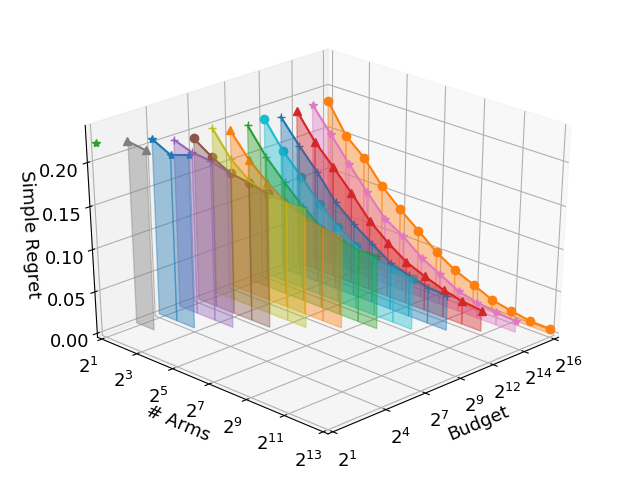
\includegraphics[width=\textwidth]{fixedbudget/figures/folder1/new_yorker.png}
	\caption{New Yorker}
	\label{appendix:fig:sh-num-arms:new_yorker}
\end{subfigure}
\label{appendix:fig:sh-num-arms}
\end{figure}

\begin{figure}
\centering
\caption{Comparison to state-of-the-art pure exploration infinite bandit algorithms}
\begin{subfigure}{0.4\textwidth}
	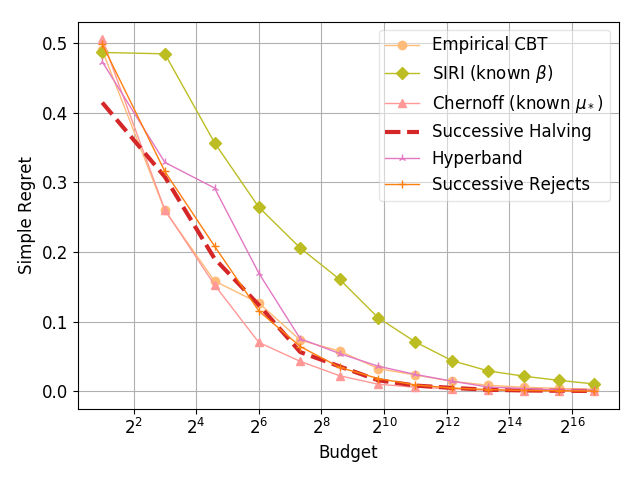
\includegraphics[width=\textwidth]{fixedbudget/figures/folder4/alpha1_beta1_unscaled.png}
	\caption{$Beta(1,1)$}
	\label{appendix:fig:sh-infinite:alpha1_beta1_unscaled}
\end{subfigure}
\quad
\begin{subfigure}{0.4\textwidth}
	\includegraphics[width=\textwidth]{fixedbudget/figures/folder4/alpha1_beta1_scaled.png}
	\caption{$Beta(1,1)$ Scaled}
	\label{appendix:fig:sh-infinite:alpha1_beta1_scaled}
\end{subfigure}
%
\begin{subfigure}{0.4\textwidth}
	\includegraphics[width=\textwidth]{fixedbudget/figures/folder4/alpha1_beta3_unscaled.png}
	\caption{$Beta(3,1)$}
	\label{appendix:fig:sh-infinite:alpha1_beta3_unscaled}
\end{subfigure}
\quad
\begin{subfigure}{0.4\textwidth}
	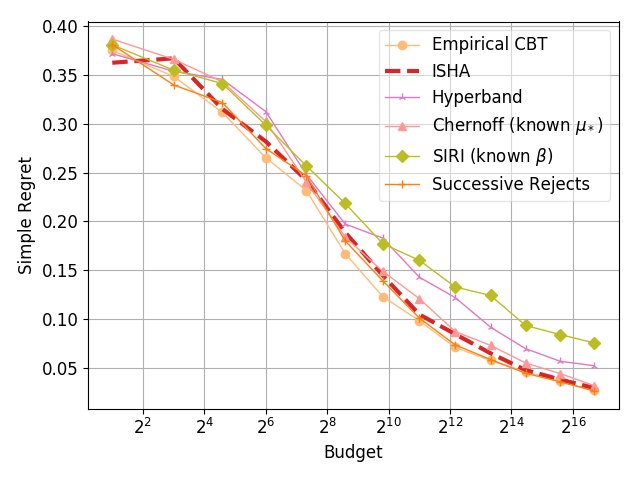
\includegraphics[width=\textwidth]{fixedbudget/figures/folder4/alpha1_beta3_scaled.png}
	\caption{$Beta(3,1)$ Scaled}
	\label{appendix:fig:sh-infinite:alpha1_beta3_scaled}
\end{subfigure}
%
\begin{subfigure}{0.4\textwidth}
	\includegraphics[width=\textwidth]{fixedbudget/figures/folder4/{TwoSpike_0.1_0.515_0.031}.png}
	\caption{TwoSpike $\pi=10^{-1}, \epsilon=\sqrt{10^{-3}}$}
	\label{appendix:fig:sh-infinite:TwoSpike_1}
\end{subfigure}
\quad
\begin{subfigure}{0.4\textwidth}
	\includegraphics[width=\textwidth]{fixedbudget/figures/folder4/{TwoSpike_0.01_0.55_0.1}.png}
	\caption{Two Spike $\pi=10^{-2}, \epsilon=\sqrt{10^{-2}}$}
	\label{appendix:fig:sh-infinite:TwoSpike_2}
\end{subfigure}
%
\begin{subfigure}{0.4\textwidth}
	\includegraphics[width=\textwidth]{fixedbudget/figures/folder4/{TwoSpike_0.001_0.658_0.316}.png}
	\caption{Two Spike $\pi=10^{-3}, \epsilon=\sqrt{10^{-1}}$}
	\label{appendix:fig:sh-infinite:TwoSpike_3}
\end{subfigure}
\quad
\begin{subfigure}{0.4\textwidth}
	\includegraphics[width=\textwidth]{fixedbudget/figures/folder4/new_yorker.png}
	\caption{New Yorker}
	\label{appendix:fig:sh-infinite:new_yorker}
\end{subfigure}
\label{appendix:fig:sh-infinite}
\end{figure}


\begin{figure}
\centering
\caption{Comparison to lil'UCB}
\begin{subfigure}{0.4\textwidth}
	\includegraphics[width=\textwidth]{fixedbudget/figures/folder5/alpha1_beta1_unscaled.png}
	\caption{$Beta(1,1)$}
	\label{appendix:fig:sh-lilucb:alpha1_beta1_unscaled}
\end{subfigure}
\quad
\begin{subfigure}{0.4\textwidth}
	\includegraphics[width=\textwidth]{fixedbudget/figures/folder5/alpha1_beta1_scaled.png}
	\caption{$Beta(1,1)$ Scaled}
	\label{appendix:fig:sh-lilucb:alpha1_beta1_scaled}
\end{subfigure}
%
\begin{subfigure}{0.4\textwidth}
	\includegraphics[width=\textwidth]{fixedbudget/figures/folder5/alpha1_beta3_unscaled.png}
	\caption{$Beta(3,1)$}
	\label{appendix:fig:sh-lilucb:alpha1_beta3_unscaled}
\end{subfigure}
\quad
\begin{subfigure}{0.4\textwidth}
	\includegraphics[width=\textwidth]{fixedbudget/figures/folder5/alpha1_beta3_scaled.png}
	\caption{$Beta(3,1)$ Scaled}
	\label{appendix:fig:sh-lilucb:alpha1_beta3_scaled}
\end{subfigure}
%
%\begin{subfigure}{0.4\textwidth}
%	\includegraphics[width=\textwidth]{figures/folder5/new_yorker.png}
%	\caption{New Yorker}
%	\label{fig:sh-lilucb:new_yorker}
%\end{subfigure}
\label{appendix:fig:sh-lilucb}
\end{figure}


\begin{figure}
\centering
\caption{Comparison to state-of-the-art explore-vs-exploit infinite bandit algorithms}
\begin{subfigure}{0.4\textwidth}
	\includegraphics[width=\textwidth]{fixedbudget/figures/folder2/alpha1_beta1_unscaled.png}
	\caption{$Beta(1,1)$}
	\label{appendix:fig:sh-unscaled-alpha1_beta1_unscaled}
\end{subfigure}
\quad
\begin{subfigure}{0.4\textwidth}
	\includegraphics[width=\textwidth]{fixedbudget/figures/folder2/alpha1_beta3_unscaled.png}
	\caption{$Beta(3,1)$}
	\label{appendix:fig:sh-unscaled-alpha1_beta3_unscaled}
\end{subfigure}
\label{appendix:fig:sh-unscaled}
\end{figure}


\begin{figure}
\centering
\caption{Anytime Performance}
\begin{subfigure}{0.4\textwidth}
	\includegraphics[width=\textwidth]{fixedbudget/figures/folder3/alpha1_beta1_unscaled.png}
	\caption{$Beta(1,1)$}
	\label{appendix:fig:sh-anytime:alpha1_beta1_unscaled}
\end{subfigure}
\quad
\begin{subfigure}{0.4\textwidth}
	\includegraphics[width=\textwidth]{fixedbudget/figures/folder3/alpha1_beta1_scaled.png}
	\caption{$Beta(1,1)$ Scaled}
	\label{appendix:fig:sh-anytime:alpha1_beta1_scaled}
\end{subfigure}
%
\begin{subfigure}{0.4\textwidth}
	\includegraphics[width=\textwidth]{fixedbudget/figures/folder3/alpha1_beta3_unscaled.png}
	\caption{$Beta(3,1)$}
	\label{appendix:fig:sh-anytime:alpha1_beta3_unscaled}
\end{subfigure}
\quad
\begin{subfigure}{0.4\textwidth}
	\includegraphics[width=\textwidth]{fixedbudget/figures/folder3/alpha1_beta3_scaled.png}
	\caption{$Beta(3,1)$ Scaled}
	\label{appendix:fig:sh-anytime:alpha1_beta3_scaled}
\end{subfigure}
%
\label{appendix:fig:sh-anytime}
\end{figure}

\begin{figure}
% \vspace{-2.5em}
\includegraphics[width=\textwidth]{fixedbudget/figures/NY_CDF.pdf}
\caption{New Yorker CDF}
\label{fig:newyorkercdf}
\end{figure}



%\end{document}


\section{Greedy-optimal Boosted Decision Trees}\label{AP-Boost}
%\documentclass{article}

% if you need to pass options to natbib, use, e.g.:
% \PassOptionsToPackage{numbers, compress}{natbib}
% before loading nips_2018

% ready for submission
%\usepackage{nips_2018}
%\usepackage[preprint]{nips_2018}

% to compile a preprint version, e.g., for submission to arXiv, add
% add the [preprint] option:
%\usepackage[preprint]{nips_2018}

% to compile a camera-ready version, add the [final] option, e.g.:
% \usepackage[final]{nips_2018}

% to avoid loading the natbib package, add option nonatbib:
% \usepackage[nonatbib]{nips_2018}

%\usepackage[utf8]{inputenc} % allow utf-8 input
%\usepackage[T1]{fontenc}    % use 8-bit T1 fonts
%\usepackage{hyperref}       % hyperlinks
%\usepackage{url}            % simple URL typesetting
%\usepackage{booktabs}       % professional-quality tables
%\usepackage{amsfonts}       % blackboard math symbols
%\usepackage{nicefrac}       % compact symbols for 1/2, etc.
%\usepackage{microtype}      % microtypography
%
%\usepackage{graphicx}
%\usepackage{algorithm}
%\usepackage{algorithmic}
%
%% Attempt to make hyperref and algorithmic work together better:
%%\newcommand{\theHalgorithm}{\arabic{algorithm}}
%
%\usepackage[title]{appendix}
%\usepackage{afterpage}
%\usepackage{amsfonts}
%\usepackage{amsmath}
%\usepackage{amsthm}
%\usepackage{amssymb}
%\usepackage{dsfont}
%\usepackage{enumitem}
%\usepackage{filecontents}
%\usepackage{todonotes}
%\usepackage{graphicx}
%\usepackage{subcaption}
%\usepackage{wrapfig}
%\usepackage{bbm}
%
%\newtheorem{assumption}{Assumption}
%\newtheorem{definition}{Definition}
%\newtheorem{theorem}{Theorem}
%\newtheorem{lemma}{Lemma}
%\newtheorem{proposition}{Proposition}
%\newtheorem{corollary}{Corollary}
%\newtheorem{remark}{Remark}
%
%\newcommand{\bP}{\mathbb{P}}
%\newcommand{\1}[1]{\mathds{1}{\left\{ #1 \right\}}}
%
%\DeclareMathOperator*{\argmin}{argmin}
%
%\newcommand{\Set}[1]{\mathchoice{\left\{ #1 \right\}}{\{ #1 \}}{\{ #1 \}}{\{ #1 \}}}

%\title{Adaptively Pruning Features for Boosted Decision Trees}

% The \author macro works with any number of authors. There are two
% commands used to separate the names and addresses of multiple
% authors: \And and \AND.
%
% Using \And between authors leaves it to LaTeX to determine where to
% break the lines. Using \AND forces a line break at that point. So,
% if LaTeX puts 3 of 4 authors names on the first line, and the last
% on the second line, try using \AND instead of \And before the third
% author name.

%\author{
%  Maryam Aziz \\
%  Northeastern University \\
%  Boston, Massachusetts, USA \\
%  \texttt{azizm@ccs.neu.edu} \\
%  \And
%  Jesse Anderton \\
%  Northeastern University \\
%  Boston, Massachusetts, USA \\
%  \texttt{jesse@ccs.neu.edu} \\
%  \And
%  Javed Aslam \\
%  Northeastern University \\
%  Boston, Massachusetts, USA \\
%  \texttt{jaa@ccs.neu.edu} \\
%}
%
%\begin{document}
%
%\maketitle

%\begin{abstract}

Boosted decision trees enjoy popularity in a variety of applications;
however, for large-scale datasets, the cost of training a decision
tree in each round can be prohibitively expensive.  Inspired by ideas
from the multi-arm bandit literature, we develop a highly efficient
algorithm for computing exact greedy-optimal decision trees,
outperforming the state-of-the-art \texttt{Quick Boost} method.  We
further develop a framework for deriving lower bounds on the problem
that applies to a wide family of conceivable algorithms for the task
(including our algorithm and \texttt{Quick Boost}), and we demonstrate
empirically on a wide variety of data sets that our algorithm is
near-optimal within this family of algorithms.  We also
derive a lower bound applicable to any algorithm solving the task, and
we demonstrate that our algorithm empirically achieves performance
close to this best-achievable lower bound.

%\end{abstract}


\section{Introduction}\label{introduction}

Boosting algorithms are among the most popular classification
algorithms in use today, e.g. in computer vision, learning-to-rank,
and text classification.  Boosting, originally introduced by
\citet{Schapire90thestrength, Freund:1995:BWL:220262.220446,
  Freund:1996:ENB:3091696.3091715}, is a family of machine learning
algorithms in which an accurate classification strategy is learned by
combining many ``weak'' hypotheses, each trained with respect to a
different weighted distribution over the training data.  These
hypotheses are learned sequentially, and at each iteration of boosting
the learner is biased towards correctly classifying the examples which
were most difficult to classify by the preceding weak hypotheses.

Decision trees \citep{Quinlan:1993:CPM:152181}, due to their simplicity
and representation power, are among the most popular weak learners
used in Boosting algorithms \citep{Freund:1996:ENB:3091696.3091715,
  Quinlan:1996:BBC:1892875.1892983}.  However, for large-scale data
sets, training decision trees across potentially hundreds of rounds of
boosting can be prohibitively expensive.  Two approaches to ameliorate
this cost include
(1) \emph{approximate decision tree training},
which aims to identify a subset of the
features and/or a subset of the training examples such that
\emph{exact} training on this subset yields a high-quality decision
tree,
and (2)
\emph{efficient exact decision tree training},
which aims to compute the greedy optimal decision tree over the entire data
set and feature space as efficiently as possible.
These two approaches complement each other:
approximate training often devolves to exact
training on a subset of the data.

  As such, we
consider the task of efficient exact decision tree learning in the
context of boosting where our primary objective is to minimize the
number of examples that must be examined for any feature in order to
perform greedy-optimal decision tree training. 
Our method
is simple to implement, and gains in feature-example efficiency directly corresponds to improvements in computation time.


The main contributions of the paper are as follows:\vspace{-0.5\baselineskip}
\begin{itemize}
\item We develop a highly efficient algorithm for computing exact
  greedy-optimal decision trees, \texttt{Adaptive-Pruning Boost}, and
  we demonstrate through extensive experiments that our method
  outperforms the state-of-the-art \texttt{Quick Boost} method.
\item We develop a constrained-oracle framework for deriving
  feature-example lower bounds on the problem that applies to a wide
  family of conceivable algorithms for the task, including our
  algorithm and \texttt{Quick Boost}, and we demonstrate that our
  algorithm is near-optimal within this family of algorithms through
  extensive experiments.
\item Within the constrained-oracle framework, we also derive a
  feature-example lower bound applicable to any algorithm solving the
  task, and we demonstrate that our algorithm empirically achieves
  performance close to this lower bound as well.
\end{itemize}

We will next expand on the ideas that underlie
our three main results above and discuss related work.

\paragraph{The Multi-Armed Bandit (MAB) Inspiration.}
Our approach to efficiently splitting decision tree nodes is based on
identifying intervals which contain the score (e.g. classifier's training accuracy) of each possible split and tightening those
intervals by observing training examples incrementally.
We can eventually exclude entire features
from further consideration because their intervals do not
overlap the intervals of the best splits.
Under this paradigm, the optimal strategy would be to assess all
examples for the best feature,
reducing its interval to an exact value,
and only then to assess examples for the remaining features
to rule them out.
Of course, we do not know in advance which feature is best.
Instead, we wish to spend our assessments optimally to identify the
best feature with the fewest assessments spent on the other features.
This corresponds well to the best arm identification problem studied
in the MAB literature. This insight inspired our training algorithm.

A ``Pure Exploration'' MAB algorithm in the ``Fixed-Confidence'' setting
\citep{DBLP:conf/icml/KalyanakrishnanTAS12,NIPS2012_4640,COLT13}
is given a set of arms (probability distributions over rewards)
and returns the arm with highest expected reward with high probability
(subsequently, WHP)
while minimizing the number of samples drawn from each arm.
Such confidence interval algorithms are generally categorized as
LUCB (Lower Upper Confidence Bounds) algorithms, because at each round
they ``prune'' sub-optimal arms whose confidence intervals do not overlap
with the most promising arm's interval until it is confident that WHP
it has found the best arm. 

In contrast to the MAB setting where one estimates the expected reward
of an arm WHP,
in the Boosting setting one can calculate the exact (training) accuracy
of a feature (expected reward of an arm) if one is willing to assess that
feature on all training examples.
When only a subset of examples are assessed, one can also calculate a
non-probabilistic ``uncertainty interval'' which is guaranteed to contain
the feature's true accuracy. This interval shrinks in proportion to the boosting weight of the assessed examples. We specialize the generic LUCB-style MAB algorithm of the best arm identification to assess examples in decreasing order of boosting weights, and to use uncertainty intervals in place of the more typical probabilistic confidence intervals.

\paragraph{Our Lower Bounds.}
We introduce two empirical lower bounds on the total number of examples needed
to be assessed in order to identify the exact greedy-optimal node for a given
set of boosting weights.
Our first lower bound is for the class of algorithms which assess feature
accuracy by testing the feature on examples in order of decreasing Boosting
weights (we call this the \emph{assessment complexity} of the problem).
We show empirically that our algorithm's performance is consistently nearly
identical to this lower bound.
%
Our second lower bound permits examples to be assessed in any order.
It requires a feature to be assessed with the minimal set of examples
necessary to prove that its training accuracy is not optimal.
This minimal set depends on the boosting weights in a given round,
from which the best possible (weighted) accuracy across all weak hypotheses
is calculated.
For non-optimal features, the minimal set is then identified using
Integer Linear Programming.




\subsection{Related Work}\label{related-work}


Much effort has gone to reducing the overall computational complexity of
training Boosting models.
In the spirit of \citet{icml2013_appel13}, which has the state-of-the-art
exact optimal-greedy boosted decision tree training algorithm \texttt{Quick Boost}
(our main competitor), we divide these attempts into three categories and
provide examples of the literature from each category: reducing
1) the set of features to focus on;
2) the set of examples to focus on; and/or
3) the training time of decision trees.
Note that these categories are independent of and parallel to each other.
For instance, 3), the focus of this work, can build a decision tree from
any subset of features or examples.
We show improvements compared to state-of-the-art algorithm both on subsets
of the training data and on the full training matrix.
Popular approximate algorithms such as
XGBoost \citep{Chen:2016:XST:2939672.2939785}
typically focus on 1) and 2)
and could benefit from using our algorithm for their training step.

Various works \citep{4270071, PaulBiswajitAthithanEtAl} focus on reducing the set of features.
\citet{busafekete:in2p3-00614564} divides features into subsets
and at each round of boosting uses adversarial bandit models to find the most promising subset for boosting. \texttt{LazyBoost} \citep{Escudero:2001:ULW:2387364.2387381} samples a subset of features uniformly at random to focus on at a given boosting round. 

Other attempts at computational complexity reduction involve sampling a set of
examples.
Given a fixed budget of examples, \texttt{Laminating}
\citep{Dubout:2014:ASL:2627435.2638580} attempts to find the best among a set of
hypotheses by testing each surviving hypothesis on a increasingly larger set of
sampled examples while pruning the worst performing half and doubling the number of examples, until it is left
with one hypthesis. It returns this hypothesis to boosting as the best one with probability $1-\delta$. The hypothesis identification part of \texttt{Laminating} is fairly identical to the best arm identification algorithm \texttt{Sequential Halving} \citep{icml2013_karnin13}. \texttt{Stochastic Gradient Boost} \citep{FriedmanStochasticGB}, and the weight trimming approach of \citet{Friedman98additivelogistic} are a few other intances of reducing the set of examples. \texttt{FilterBoost} \citep{NIPS2007_3321} uses an oracle to sample a set of examples from a very large dataset and uses this set to train a weak learner.

Another line of research focuses on reducing the training time of decision trees
\citep{implementing-decision-trees-and-forests-on-a-gpu, articleWuEtAl}.
More recently, \citet{icml2013_appel13} proposed \texttt{Quick Boost}, which
trains decision tree as weak learners while pruning underperforming
features earlier than a classic Boosting algorithm would.
They build their algorithm on the insight that the (weighted) error rate of
a feature when trained on a subset of examples can be used to bound its error
rate on all examples.
This is because the error rate is simply the normalized sum of the weights of the misclassified examples; if one supposes that all unseen examples may be
correctly classified, that yields a lower bound on the error rate.
If this lower bound is above the best observed error rate of a feature
trained on all examples, the underperforming feature may be pruned and no
more effort spent on it.

Our \texttt{Adaptive-Pruning Boost} algorithm carries forward the ideas
introduced by \texttt{Quick Boost}.
In contrast to \texttt{Quick Boost},
our algorithm is parameter-free and adaptive.
Our algorithm uses fewer training examples and thus faster training CPU time than
\texttt{Quick Boost}.
It works by gradually adding weight to the
``winning'' feature with the smallest upper bound on, e.g., its error rate
and the ``challenger'' feature with smallest lower bound,
until all challengers are pruned.
We demonstrate consistent improvement over \texttt{Quick Boost} on a
variety of datasets,
and show that when speed improvements are more modest this is due to
\texttt{Quick Boost} approaching the lower bound more tightly rather than
due to our algorithm using more examples than are necessary.
Our algorithm is consistently nearly-optimal in terms of the lower bound
for algorithms which assess examples in weight order,
and this lower bound in turn is close to the global lower bound.
Experimentally, we show that the reduction in total assessed examples
also reduces the CPU time.



\subsubsection{Setup and Notation}
We adopt the setup, 
description and notation of~\citet{icml2013_appel13} for ease of
comparison.  

\paragraph {A Generic Boosting Algorithm.}
Boosting algorithms train a linear combination of classifiers
$\mathcal{H}_T(x)=\sum^T_t {\alpha_t h_t(x)}$
such that an error function $\mathcal{E}$ is minimized by optimizing scalar
$\alpha_t$ and the weak learner $h_t(x)$ at round $t$.
Examples $x_i$ misclassified by $h_t(x)$ are assigned ``heavy'' weights $w_i$
so that the algorithm focuses on these heavy weight examples when training weak
learner $h_{t+1}(x)$ in round $t+1$.
Decision trees, defined formally below, are often used as weak learners.

\paragraph {Decision Tree.}  A binary decision tree $h_{\textit{Tree}}(x)$ is a
tree-based classifier where every non-leaf node is a decision stump
$h(x)$.  A decision stump can be viewed as a tuple $(p, k, \tau)$ of a
polarity (either $+1$ or $-1$), the feature column index, and
threshold, respectively, which predicts a binary label from the set
$\{+1, -1\}$ for any input $x \in \mathbb{R}^K$ using the function
$h(x) \equiv p\mathop{\mathrm{sign}}(x[k] - \tau)$.

A decision tree $h_{\textit{Tree}}(x)$ is trained, top to bottom, by
``splitting'' a node, i.e. selecting a stump $h(x)$ that optimizes
some function such as error rate, information gain, or GINI impurity.  
While this chapter focuses on selecting stumps based on
error rate, we intend to extend our work to other measures.
Our algorithm \texttt{Adaptive-Pruning Stump} (Algorithm~\ref{adaptive-pruning-stump}), a subroutine of \texttt{Adaptive-Pruning Boost} (Algorithm~\ref{boosting}), trains a decision stump $h(x)$ with
fewer total example assessments than its analog, the subroutine of the-state-of-the-art algorithm
\texttt{Quick Boost}, does. Note that \texttt{Adaptive-Pruning Stump} used iteratively can train a decision tree, but for simplicity we assume our weak learners are binary decision stumps.
While we describe \texttt{Adaptive-Pruning Stump} for
binary classification, the reasoning also applies to multi-class data.
% the
%decision stump ultimately differentiates between one class and a group of
%classes (a binary classification).

To describe how \texttt{Adaptive-Pruning Stump} trains a stump
we need a few definitions.
Let $n$ be the total number of examples, and $m \le n$ some number of examples
on which a stump has been trained so far.
We will assume that Boosting provides the examples in decreasing weight
order.
This order can be maintained in $O(n)$ time in the presence of Boosting weight updates
because examples which are correctly classified do not change their relative
weight order, and examples which are incorrectly classified do not change their
relative weight order; a simple merge of these two groups suffices.
We can therefore number our examples from 1 to $n$ in decreasing weight order.
Furthermore,
\begin{itemize}[topsep=0pt,itemsep=0pt]
\item let $Z_m := \sum_{i=1}^m {w_i}$ be sum of the weights of first $m$ (heaviest) examples, and
\item let $\epsilon_m := \sum_{i=1}^m {w_i \mathbbm{1} \{h(x_i) \ne y_i\}}$ be the sum of the weights of the examples from the first $m$ which are misclassified by the stump $h(x)$.
\end{itemize}

The weighted error rate for stump $j$ on the first $m$ examples is then
$E^j_m := \epsilon_m^j / Z_m$.





\subsection{Algorithm}\label{alg}
\texttt{Adaptive-Pruning Stump} prunes features based on
exact intervals (which we call uncertainty intervals) and returns the best feature
deterministically.
To do this we need lower bounds and upper bounds on the stump's
training error rate. 
Our lower bound assumes that all unseen examples are classified
correctly and our upper bound assumes that all unseen examples are classified
incorrectly.
We define $L_m^j$ as the lower bound on the error rate for
stump $j$ on all $n$ examples, when computed on the first $m$ examples,
and $U_m^j$ as the corresponding upper bound.
%\begin{itemize}
%\item $L_m^j := \epsilon_m^j / Z_n$ is the lower bound on the error rate for
%	stump $j$ on all $n$ examples, when computed on the first $m$ examples, and
%\item $U_m^j := (\epsilon_m^j + Z_n - Z_m) / Z_n$ is the upper bound for stump $j$ when computed on the first $m$ examples.
%\end{itemize}
For any $1 \le m \le n$, we define,
%\begin{align}
%$L_m^j \le E_n^j \le U_m^j$
%\end{align}
using $c^j_i := \mathbbm{1} \{h_j(x_i) \ne y_i\}$ to indicate
whether stump $j$ incorrectly classifies example $i$,
\begin{align*}
	L_m^j :=
%	= \frac{\epsilon^j_m}{Z_n}
%	\underbrace{
	 \frac{1}{Z_n}
		\sum_{i=1}^m {w_i c^j_i}
%		}_{L_m^j}
%\\
	\le  
	\underbrace{
	\frac{1}{Z_n} 
%	\left(
%		\sum_{i=1}^m {w_i c^j_i}
%		+ \sum_{i=m+1}^n {w_i c^j_i}
		\sum_{i=1}^n {w_i c^j_i}
%		\right)
	}_{E_n^j}
%\\
	\le  \frac{1}{Z_n}\left(
		\epsilon^j_m
		+ \sum_{i=m+1}^n w_i
		\right)
%\\
	=
%	  \underbrace{
	\frac{1}{Z_n}\left(
		\epsilon^j_m
		+ (Z_n - Z_m)
		\right)
%		}_{U_m^j}
		=: U_m^j.
\end{align*}
%
For any two stumps $i$ and $j$ when numbers $m$ and $m'$ exist
such that $L_m^i > U_{m'}^j$ then we can safely discard stump $i$, as it cannot
have the lowest error rate.
This extension of the pruning rule used by \citet{icml2013_appel13}
permits each feature to have its own interval of possible error
rates, and permits us to compare features for pruning without first
needing to assess all $n$ examples for any feature
(\texttt{Quick Boost}'s subroutine requires the
current-best feature to be tested on all $n$ examples).

Now we describe our algorithm in detail; see the
listing in Algorithm~\ref{adaptive-pruning-stump}.
We use $f_k$ to denote an object which stores all decision stumps $h(x)$ for feature
$x[k]$.
Recall that $x \in \mathbb{R}^K$ and that $x[k]$ is the $k_{th}$ feature of $x$,
for $k \in \{ 1, \dots, K \}$.
$f_k$ has method $assess(batch)$, when given a ``batch'' of examples, updates
$L_m$, $E_m$,  $U_m$ (defined above) for all decision stumps of feature $x[k]$ based
on the examples in the batch.
It also has methods $LB()$ and $UB()$, which report the $L_m$ and $U_m$ for the
single hypothesis with smallest error $E_m$ on the $m$ examples seen so far,
and $bestStump()$, which returns the hypothesis with smallest error $E_m$.

\texttt{Adaptive-Pruning Stump} proceeds until there is some feature $k^*$ whose upper bound
is below the lower bounds for all other features.
We then know that the best hypothesis uses feature $k^*$.
We assess any remaining unseen examples
for feature $k^*$ in order to identify the best threshold and polarity
and to calculate $E^{k^*}_n$.
Thus, our algorithm always finds the exact greedy-optimal hypothesis.

In order to efficiently compare two features $i$ and $j$ to decide whether
to prune feature $i$,
we want to ``add'' the minimum weight to these arms to
possibly obtain that $L_m^i > U_{m'}^j$.
The most efficient way to do this is to test each feature against
a batch of the heaviest unseen examples whose weight is at least
the gap $U_{m'}^j - L_m^i$.
This permits us to choose batch sizes adaptively, based on the minimum weight
needed to prune a feature given the current boosting weights and the
current uncertainty intervals for each arm.
We note that our ``weight order'' lower bound on the sample complexity of the
problem in the next section is also calculated based on this insight.
This is in contrast to \texttt{Quick Boost}, which accepts parameters to
specify the total number of batches and the weight to use for initial estimates;
the remaining weight is divided evenly among the batches.
When the number of batches chosen is too large, the run time of a training
round approaches $O(n^2)$; when it is too small, the run time approaches
that of assessing all $n$ examples.

\begin{wrapfigure}{R}{0.5\textwidth}
\vspace{-2.5em}
\begin{minipage}[t]{0.5\textwidth}
\begin{algorithm}[H]
\caption{\texttt{Adaptive-Pruning Stump}}\label{adaptive-pruning-stump}
\begin{algorithmic}
   \STATE {\bfseries Input:} Examples \{$x_1, \dots, x_n$\}, Labels \{$y_1, \dots, y_n$\}, Weights $\{w_{1},\dots,w_{n}\}$
    \STATE {\bfseries Output:} $h(x)$  
    \STATE $m \gets$ min. index s.t. $Z_m \ge 0.5$
    \FOR {$k = 1$ {\bfseries to} $K$}
        \STATE $f_k.assess([x_1, \dots, x_m]); m_k \gets m$
    \ENDFOR
    \STATE $a \gets k$ with min $f_k.UB()$
    \STATE $b \gets k \ne a$ with min $f_k.LB()$
    \WHILE {$f_a.UB() > f_b.LB()$}
        \STATE $gap \gets f_a.UB() - f_b.LB()$
        \STATE $m \gets$ min index s.t. $Z_m \ge Z_{m_a} + gap$
        \STATE $f_a.assess([x_{m_a+1}, \dots, x_m]); m_a \gets m$
        \STATE $gap \gets f_a.UB() - f_b.LB()$
        \IF {$gap > 0$}
            \STATE $m \gets$ min index s.t. $Z_m \ge Z_{m_b} + gap$
            \STATE $f_b.assess([x_{m_b+1}, \dots, x_m]); m_b \gets m$
        \ENDIF
        \IF {$f_a.UB() < f_b.UB()$}
            \STATE $a \gets b$
        \ENDIF
        \STATE $b \gets k \ne a$ with min $f_k.LB()$
    \ENDWHILE
    \STATE {\bfseries return} $h(x) := f_a.bestStump()$
\end{algorithmic}
\end{algorithm}
\end{minipage}
%
\begin{minipage}[t]{0.5\textwidth}
\begin{algorithm}[H]
\caption{\texttt{Adaptive-Pruning Boost}}\label{boosting}
\begin{algorithmic}
   \STATE {\bfseries Input:} Instances \{$x_1, \dots, x_n$\}, Labels \{$y_1, \dots, y_n$\}
   \STATE {\bfseries Output:} $\mathcal{H}_T(x)$
   \STATE {\bfseries Initialize Weights:} $\{w_{1},\dots,w_{n}\}$   \FOR{$t=1$ {\bfseries to} $T$}
   \STATE Train Decision Tree $h_{Tree}(x)$ one node at a time by calling \texttt{Adaptive-Pruning Stump}
   \STATE Choose $\alpha_t$ and update $\mathcal{H}_t(x)$
   \STATE Update and Sort (in descending order) $w$
   \ENDFOR
\end{algorithmic}
\end{algorithm}
\end{minipage}
\vspace{-6em}
\end{wrapfigure}

At each round, \texttt{Adaptive-Pruning Boost} trains a decision tree
in Algorithm~\ref{boosting} by calling the subroutine
\texttt{Adaptive-Pruning Stump} of Algorithm~\ref{adaptive-pruning-stump}.

\paragraph{Implementation Details.}
The $f_k.assess()$ implementation is shared across all algorithms.
 For $b$ batches of exactly $m$ examples each on a feature $k$ with $v$ distinct
 values, our implementation of $f_k.assess$ takes $O(b m \log (m + v))$
 operations.
 We maintain an ordered list of intervals of thresholds for each feature with
 the feature values for the examples assessed so far lying on the interval
 boundaries.
 Any threshold in the interval will thus have the same performance on all
 examples assessed so far.
 To assess a batch of examples, we sort the examples in the batch by feature
 value and then split intervals as needed and calculate scores for the
 thresholds on each interval in time linear in the batch size and number of
 intervals.

Note also that maintaining the variables $a$ and $b$ requires a
single heap, and that in many iterations of the \texttt{while} loop we can
update these variables from the heap in constant time
(e.g. when $b$ has not changed, when $a$ and $b$ are simply swapped,
or when $b$ can be pruned).

\subsection{Lower Bounds}\label{lb}


\begin{wrapfigure}{R}{0.5\textwidth}
\centering
\begin{subfigure}{.5\textwidth}
\includegraphics[width=\linewidth]{decisiontree/figures/result4_elb_w4a}
\end{subfigure}
\begin{subfigure}{.5\textwidth}
\includegraphics[width=\linewidth]{decisiontree/figures/result4_elb_a6a}
\end{subfigure}
\caption{Lower Bounds versus Upper Bounds. Datasets W4A (top) and A6A (bottom) were used with trees of depth 1.
The y-axis is the \emph{fraction of the gap}
between the exact lower bound
(at zero) and the full corpus size (at one) which an algorithm used in a
given round.
Non-cumulative example assessments are plotted for every 10 rounds.
}
\label{fig:elb}
\vspace{-2em}
\end{wrapfigure}



We compare \texttt{Adaptive-Pruning Boost} against two lower bounds, defined empirically based
on the boosting weights in a given round.
In our \emph{weight order lower bound}, we consider the minimum number
of examples required to determine that a given feature is underperforming
with the assumption that examples will be assessed in order of decreasing
boosting weight.
Our \emph{exact lower bound} permits examples to be assessed in any order,
and so bounds any possible algorithm which finds the best-performing feature.

\paragraph{Weight Order Lower Bound.}
For this bound, we first require that \texttt{Adaptive-Pruning Stump} selects the feature with
minimal error.
In the case of ties, an optimal feature may be chosen arbitrarily.
\texttt{Adaptive-Pruning Stump} need to assess every example for the returned
feature in order for \texttt{Adaptive-Pruning Boost} to calculate $\alpha$ and update weights $w$ , so the lower
bound for the returned feature is simply the total number of examples $n$.

Let $k^*$ be the returned feature, and $E^*$ its error rate
when assessed on all $n$ examples.
For any feature $k \ne k^*$ which is not returned, we need to prove that it is
underperforming (or tied with the best feature).
Let $J_k$ be the set of decision stumps which use feature $k$;
then we need to find the smallest value $m$ such that for all stumps
$j \in J_k$, we have $L^j_m \ge E^*$.
Our lower bound is simply 
$	LB_{wo} :=
	n + \sum_{k \ne k^*} \min \Set{m : \forall j \in J_k, L^j_{m} \ge E^*}$.
We present results in Figure~\ref{fig:wolb} showing that \texttt{Adaptive-Pruning Boost}
achieves this bound on a variety of datasets.
\texttt{Quick Boosting}, in contrast, sometimes approaches
this bound but often uses more examples than necessary.


\paragraph{Exact Lower Bound.}
In order to test the idea that adding examples in weight order is nearly optimal,
and to provide a lower bound on \emph{any} algorithm which finds the
optimal stump, we also present an exact lower bound on the problem.
Like the weight order lower bound, this bound is defined in terms of the boosting
weights in a given round; unlike it, examples may be assessed in any order.
It is not clear how one might achieve the exact lower bound without incurring an
additional cost in time.
We leave such a solution to future work.
However, we show in Figure~\ref{fig:elb} that this bound is, in fact,
very close to the weight order lower bound.

For the exact lower bound, we still require the selected feature $k^*$ to be
assessed against all examples; this is imposed by the boosting algorithm.
For any other feature $k \ne k^*$, we simply need the size of the smallest
set of examples which would prune the feature (or prove it is tied with $k^*$).
We will use $M \subseteq \Set{1,\dots,n}$ to denote a set of indexes of examples
assessed for a given feature,
and $L^j_M$ to denote the lower bound of stump $j$ when assessed on the
examples in subset $M$.
This bound, then, is
%\begin{align}
$	LB_{exact} :=
	n + \sum_{k \ne k^*} \min_{M : L^j_M \ge E^*} |M|$.
%\end{align}

We identify the examples included in the smallest subset $M$
for a given feature $k \ne k^*$ using integer linear programming.
We define binary variables $c_1,\dots,c_n$, where $c_i$ indicates whether example
$i$ is included in the set $M$.
We then create a constraint for each stump $j \in J_k$ defined for feature $k$
which requires that the stump be proven underperforming.
Our program, then, is:
$
%\begin{align}
	\texttt{Minimize } 
%	&
%	\\ \nonumber
%	 & 
	 \sum_{i=1}^n c_i
%	\\ \nonumber
	\texttt{ s.t. }
%	& 
	c_i \in \Set{0,1}
		~~~ \forall i 
%		\in \Set{1,\dots,n}
, \texttt{ and }
%	\\ \nonumber
%	& 
	\sum_{i=1}^n c_i w_i \1{ h_j(x_i) \ne y_i }
		\ge E^*
		~~~ \forall j \in J_k$.
%\end{align}

\paragraph{Discussion.}
Figure~\ref{fig:elb} shows a non-cumulative comparison of our weight order lower bound to the global lower bound. Minimizing the global lower bound function mentioned above is computationally expensive. For this reason we used binary class datasets of moderate size and trees of depth 1 as weak leaners, but we have no reason to believe that the technique would not work for deeper trees and multi-class datasets. Refer to Table~\ref{datasets} for details of datasets.
The weight order lower bound and \texttt{Adaptive-Pruning Boost} 
are within 10-20\% of the exact lower bound,
but \texttt{Quick Boost} often uses half to all of the unnecessary
training examples in a given round.

\subsection{Experiments}
We experimented with shallow trees on various binary and multi-class datasets.
We report both assessment complexity and CPU time complexity for each dataset. Though \texttt{Adaptive-Pruning Boost} is a general Boosting algorithm, we experimented with the following class of algorithms (1) Boosting exact greedy-optimal decision trees and (2) Boosting approximate decision trees.

Each algorithm was run with either the state-of-the-art method (\texttt{Quick Boost}) or our decision tree training method (\texttt{Adaptive-Pruning Boost}), apart from the case of Figure~\ref{fig:wolb} that also uses the brute-force decision tree search method (\texttt{Classic AdaBoost}). The details of our datasets are in Table~\ref{datasets}. For datasets SATIMAGE, W4A, A6A, and RCV1 tree depth of three was used and for MNIST Digits tree depth of four was used (as in \citet{icml2013_appel13}). Train and test error results are provided as supplementary material.

\begin{table*}[ht]
\caption{The datasets used in our experiments.}
\label{datasets}
\vskip 0.15in
\begin{center}
\begin{small}
\begin{sc}
\begin{tabular}{llccc}
\toprule
Dataset & Source & Train / Test Size & Total Features & Classes\\
\midrule
a6a & \citet{Platt:1999:FTS:299094.299105} & 11220 / 21341 & 123 & 2 \\
MNIST Digits & \citet{726791} & 60000 / 10000 & 780 & 10 \\
rcv1 (Binary) & \citet{Lewis:2004:RNB:1005332.1005345} & 20242 / 677399 & 47236 & 2 \\
satimage & \citet{991427} & 4435 / 2000 & 36 & 6 \\
w4a & \citet{Platt:1999:FTS:299094.299105} & 7366 / 42383 & 300 & 2 \\
\bottomrule
\end{tabular}
\end{sc}
\end{small}
\end{center}
\vskip -0.1in
\end{table*}


\paragraph{Boosting Exact Greedy-Optimal Decision Trees.}
We used \texttt{AdaBoost} for exact decision tree training.
Figure~\ref{fig:wolb} shows the total number of example assessments used by AdaBoost when it uses three different decision trees building methods described above. In all of these experiments, our algorithm, \texttt{Adaptive-Pruning Boost}, not only consistently beats \texttt{Quick Boost} but it also almost matches the weight order lower bound. The \texttt{Classic AdaBoost} can be seen as the upper bound on the total number of example assessments.

Table~\ref{complexity-exact-results} shows that CPU time improvements correspond to example-assessments improvements for \texttt{Adaptive-Pruning Boost} for all our datasets, except for RCV1. This could be explained by Figure~\ref{fig:wolb} wherein \texttt{Quick Boost} is seen approaching the lower bound for this particular dataset. While \texttt{Adaptive-Pruning Boost} is closer to the lower bound, its example-assessments improvements are not enough to translate to CPU time improvements.

 \begin{figure*}[ht]
\centering
\begin{subfigure}{.31\linewidth}
\includegraphics[width=\linewidth]{decisiontree/figures/result3_wolb_a6a}
\end{subfigure}
\begin{subfigure}{.31\linewidth}
\includegraphics[width=\linewidth]{decisiontree/figures/result3_wolb_mnist}
\end{subfigure}
\begin{subfigure}{.31\linewidth}
\includegraphics[width=\linewidth]{decisiontree/figures/result3_wolb_rcv1}
\end{subfigure}
\begin{subfigure}{.31\linewidth}
\includegraphics[width=\linewidth]{decisiontree/figures/result3_wolb_satimage}
\end{subfigure}
\begin{subfigure}{.31\linewidth}
\includegraphics[width=\linewidth]{decisiontree/figures/result3_wolb_w4a}
\end{subfigure}
\caption{We report the total number of assessments at various boosting rounds used by the algorithms, as well as the weight order lower bound. In all of these experiments, our algorithm, \texttt{AP Boost}, not only consistently beats \texttt{Quick Boost} but it also almost matches the lower bound.}
\label{fig:wolb}
\end{figure*}

\begin{table*}[ht]
\caption{Computational Complexity for AdaBoost.
All results are for 500 rounds of boosting except MNIST (300 rounds) and RCV1 (400 rounds).}
\label{complexity-exact-results}	
\vskip 0.15in
\begin{center}
\begin{small}
\begin{sc}
\begin{tabular}{llccrccr}
\toprule
& & \multicolumn{3}{c}{CPU Time in Seconds} & \multicolumn{3}{c}{\# Example Assessments} \\
Dataset & Boosting & AP-B & QB & Improv. & AP-B & QB & Improv. \\
\midrule
a6a & AdaBoost & 4.49e+02 & 4.46e+02 & 5.3\% & 1.69e+09 & 1.83e+09 & 7.8\% \\
%
mnist & AdaBoost & 6.32e+05 & 6.60e+05 & 4.2\% & 3.52e+11 & 3.96e+11 & 11.1\% \\
%
rcv1 & AdaBoost & 1.58e+05 & 1.58e+05 & -0.5\% & 6.15e+11 & 6.58e+11 & 6.5\% \\
%
satimage & AdaBoost & 9.21e+02 & 1.19e+03 & 18.9\% & 8.64e+08 & 1.11e+09 & 22.5\% \\
%
w4a & AdaBoost & 3.03e+02 & 3.96e+02 & 27.1\% & 1.69e+09 & 2.41e+09 & 29.8\% \\
\midrule
Mean &  & &  & 11\% & & & 15.54\% \\
\bottomrule
\end{tabular}
\end{sc}
\end{small}
\end{center}
\vskip -0.1in
\end{table*}



\paragraph{Boosting Approximate Decision Trees.}
We used two approximate boosting algorithms.
We experimented with Boosting with Weight-Trimming 90\% and 99\% \citep{Friedman98additivelogistic}, wherein the weak hypothesis is trained only on 90\% or 99\% of the weights, and LazyBoost 90\% and 50\% \citep{Escudero:2001:ULW:2387364.2387381} wherein the weak hypothesis is trained only on 90\% or 50\% randomly selected features. Table~\ref{complexity-approx-results} shows that the CPU time improvements correspond to assessment improvements.

Note that approximate algorithms like XGBoost of \cite{Chen:2016:XST:2939672.2939785} are not competitors to \texttt{Adaptive-Pruning Boost} but rather potential ``clients'' because such algorithms train on a subset of the data. Therefore, they are not appropriate baselines to our method.
\begin{table*}[ht]
\caption{Computational Complexity for LazyBoost and Boosting with Weight Trimming.
All results are for 500 rounds of boosting except MNIST (300 rounds) and RCV1 (400 rounds).}
\label{complexity-approx-results}	
\vskip 0.15in
\begin{center}
\begin{small}
\begin{sc}
\begin{tabular}{llccrccr}
\toprule
& & \multicolumn{3}{c}{CPU Time in Seconds} & \multicolumn{3}{c}{\# Example Assessments} \\
Dataset & Boosting & AP-B & QB & Improv. & AP-B & QB & Improv. \\
\midrule
a6a & LazyBoost (0.5) & 1.86e+02 & 1.95e+02 & 4.8\% & 8.48e+08 & 9.22e+08 & 8.1\%  \\
mnist & LazyBoost (0.5) & 4.44e+05 & 4.57e+05 & 2.8\% & 1.84e+11 & 2.05e+11 & 10.3\% \\
rcv1 & LazyBoost (0.5) & 7.86e+04 & 7.54e+04 & -4.2\% & 3.18e+11 & 3.29e+11 & 3.4\% \\
satimage & LazyBoost (0.5) & 4.70e+02 & 5.48e+02 & 14.2\%  & 5.17e+08 & 6.11e+08 & 15.4\%  \\
w4a & LazyBoost (0.5) & 1.15e+02 & 1.58e+02 & 26.8\% & 8.61e+08 & 1.22e+09 & 29.3\% \\
\midrule
Mean &  & &  & 8.68\% & & & 13.18\% \\
\midrule
a6a & LazyBoost (0.9) & 3.28e+02 & 3.48e+02 & 5.6\%  & 1.51e+09 & 1.64e+09 & 7.7\%  \\
mnist & LazyBoost (0.9) & 7.63e+05 & 7.86e+05 & 2.9\% & 3.24e+11 & 3.62e+11 & 10.5\% \\
rcv1 & LazyBoost (0.9) & 1.38e+05 & 1.37e+05 & -1.0\% & 5.60e+11 & 5.93e+11 & 5.6\% \\
satimage & LazyBoost (0.9) & 7.37e+02 & 8.89e+02 & 17.1\%  & 8.05e+08 & 1.01e+09 & 20\%  \\
w4a & LazyBoost (0.9) & 2.04e+02 & 2.82e+02 & 27.7\% & 1.52e+09 & 2.19e+09 & 30.5\% \\
\midrule
Mean &  & &  & 10.54\% & & & 14.94\% \\
\midrule
a6a & Wt. Trim (0.9) & 2.69e+02 & 2.69e+02 & 0\%  & 1.23e+09 & 1.24e+09 & 1.4\%  \\
mnist & Wt. Trim (0.9) & 7.91e+05 & 9.49e+05 & 16.6\% & 4.61e+11 & 4.61e+11 & 0.0\% \\
rcv1 & Wt. Trim (0.9) & 8.87e+04 & 8.95e+04 & 0.9\%  & 3.65e+11 & 3.79e+11 & 3.6\% \\
satimage & Wt. Trim (0.9) & 9.87e+02 & 9.76e+02 & -1.2\%  & 1.26e+09 & 1.26e+09 & 0.1\%  \\
w4a & Wt. Trim (0.9) & 1.88e+02 & 1.96e+02 & 4.1\% & 1.40e+09 & 1.43e+09 & 2.5\% \\
\midrule
Mean &  & &  & 4.74\% & & & 1.52\% \\
\midrule
a6a & Wt. Trim (0.99) & 3.34e+02 & 3.38e+02 & 1.3\%  & 1.54e+09 & 1.58e+09 & 2.6\%  \\
mnist & Wt. Trim (0.99) & 7.46e+05 & 7.27e+05 & -2.6\% & 3.18e+11 & 3.33e+11 & 4.8\% \\
rcv1 & Wt. Trim (0.99) & 1.38e+05 & 1.37e+05 & -1.0\% & 5.61e+11 & 5.86e+11 & 4.4\% \\
satimage & Wt. Trim (0.99) & 6.49e+02 & 6.68e+02 & 2.9\%  & 7.01e+08 & 7.39e+08 & 5.1\%  \\
w4a & Wt. Trim (0.99) & 1.91e+02 & 2.03e+02 & 6.0\% & 1.44e+09 & 1.52e+09 & 5.3\% \\
\midrule
Mean &  & &  & 1.48\% & & & 4.7\% \\
\bottomrule
\end{tabular}
\end{sc}
\end{small}
\end{center}
\vskip -0.1in
\end{table*}







\subsection{Conclusion}
In this chapter, we introduced an efficient exact greedy-optimal algorithm, \texttt{Adaptive-Pruning Boost}, for boosted decision trees. Our experiments on various datasets show that our algorithm use fewer total example assessments compared to the-state-of-the-art algorithm \texttt{Quick Boost}. We further showed that \texttt{Adaptive-Pruning Boost} almost matches the lower bound for its class of algorithms and the global lower bound for any algorithm.


\clearpage


%%%%%%%%%%%%%%%%%%%%%%%%%%%%%%%%%%%%%%%%%%%%%%%%%%%%%%%%%%%%%%%%%%%%%%%%%%%%%%%
%%%%%%%%%%%%%%%%%%%%%%%%%%%%%%%%%%%%%%%%%%%%%%%%%%%%%%%%%%%%%%%%%%%%%%%%%%%%%%%
% DELETE THIS PART. DO NOT PLACE CONTENT AFTER THE REFERENCES!
%%%%%%%%%%%%%%%%%%%%%%%%%%%%%%%%%%%%%%%%%%%%%%%%%%%%%%%%%%%%%%%%%%%%%%%%%%%%%%%
%%%%%%%%%%%%%%%%%%%%%%%%%%%%%%%%%%%%%%%%%%%%%%%%%%%%%%%%%%%%%%%%%%%%%%%%%%%%%%%
\clearpage

%\begin{appendices}
\subsection{Additional Results}
\subsubsection{Train and Test Error for AdaBoost}
Table~\ref{tbl:AdaBoostTestTrainErrors} reports test and train errors at various Boosting rounds. Our algorithm achieves the test and train error in fewer total number of example assessments, compared to \texttt{Quick Boost}. Note that both algorithms, except in the case of RCV1, have the same test and train error at a given round, as they should because both train identical decision trees. The case of RCV1 is due to the algorithms picking a weak learner arbitrarily in case of ties, without changing the overall results significantly.
\begin{table*}[ht]
\caption{AdaBoost results,
reported at rounds 100, 300 and 500 (400 for RCV1).}
\label{tbl:AdaBoostTestTrainErrors}
\vskip 0.15in
\begin{center}
\begin{small}
\begin{sc}
\begin{tabular}{lccccccccc}
\toprule
	& \multicolumn{3}{c}{100}
	& \multicolumn{3}{c}{300}
	& \multicolumn{3}{c}{400/500}
	\\
Alg: Data & \# Assess. & Train & Test & \# Assess. & Train & Test & \# Assess. & Train & Test \\
\midrule
AP-B: a6a & 3.35e+08 & 0.142 & 0.155 & 1.02e+09 & 0.131 & 0.157 & 1.69e+09 & 0.128 & 0.160 \\
QB: a6a & 3.57e+08 & 0.142 & 0.155 & 1.09e+09 & 0.131 & 0.157 & 1.83e+09 & 0.128 & 0.160 \\
AP-B: mnist & 1.26e+11 & 0.106 & 0.111 & 3.52e+11 & 0.057 & 0.064 & --- & --- & --- \\
QB: mnist & 1.36e+11 & 0.106 & 0.111 & 3.96e+11 & 0.057 & 0.064 & --- & --- & --- \\
AP-B: rcv1 & 1.73e+11 & 0.027 & 0.059 & 4.83e+11 & 0.005 & 0.047 & 6.15e+11 & 0.001 & 0.044 \\
QB: rcv1 & 1.85e+11 & 0.029 & 0.061 & 5.13e+11 & 0.004 & 0.047 & 6.58e+11 & 0.001 & 0.046 \\
AP-B: satimage & 1.98e+08 & 0.113 & 0.150 & 5.46e+08 & 0.070 & 0.121 & 8.64e+08 & 0.049 & 0.109 \\
QB: satimage & 2.20e+08 & 0.113 & 0.150 & 6.61e+08 & 0.070 & 0.121 & 1.11e+09 & 0.049 & 0.109 \\
AP-B: w4a & 3.92e+08 & 0.011 & 0.019 & 1.07e+09 & 0.006 & 0.018 & 1.69e+09 & 0.006 & 0.018 \\
QB: w4a & 4.64e+08 & 0.011 & 0.020 & 1.45e+09 & 0.006 & 0.018 & 2.41e+09 & 0.006 & 0.018 \\
\bottomrule
\end{tabular}
\end{sc}
\end{small}
\end{center}
\vskip -0.1in
\end{table*}


\subsection{Train and Test Error for LazyBoost and Weight Trimming}
\begin{table*}[ht]
\caption{Performance for A6A}
\label{tbl:perf-a6a}
\vskip 0.15in
\begin{center}
\begin{small}
\begin{sc}
\begin{tabular}{lccccccccc}
\toprule
	& \multicolumn{3}{c}{100}
	& \multicolumn{3}{c}{300}
	& \multicolumn{3}{c}{500}
	\\
 & \# Assess. & Train & Test & \# Assess. & Train & Test & \# Assess. & Train & Test \\
\midrule
AP LazyBoost (0.5) & 1.69e+08 & 0.145 & 0.156 & 5.11e+08 & 0.134 & 0.159 & 8.48e+08 & 0.129 & 0.160 \\
QB LazyBoost (0.5) & 1.80e+08 & 0.145 & 0.157 & 5.50e+08 & 0.137 & 0.158 & 9.22e+08 & 0.132 & 0.160 \\
AP LazyBoost (0.9) & 2.99e+08 & 0.141 & 0.156 & 9.07e+08 & 0.133 & 0.157 & 1.51e+09 & 0.130 & 0.159 \\
QB LazyBoost (0.9) & 3.18e+08 & 0.141 & 0.156 & 9.75e+08 & 0.133 & 0.157 & 1.64e+09 & 0.130 & 0.159 \\
AP Wt. Trim (0.9) & 2.45e+08 & 0.151 & 0.157 & 7.35e+08 & 0.151 & 0.157 & 1.23e+09 & 0.151 & 0.157 \\
QB Wt. Trim (0.9) & 2.49e+08 & 0.151 & 0.157 & 7.46e+08 & 0.151 & 0.157 & 1.24e+09 & 0.151 & 0.157 \\
AP Wt. Trim (0.99) & 3.16e+08 & 0.141 & 0.156 & 9.34e+08 & 0.132 & 0.157 & 1.54e+09 & 0.126 & 0.158 \\
QB Wt. Trim (0.99) & 3.28e+08 & 0.141 & 0.156 & 9.62e+08 & 0.132 & 0.157 & 1.58e+09 & 0.126 & 0.160 \\
\bottomrule
\end{tabular}
\end{sc}
\end{small}
\end{center}
\vskip -0.1in
\end{table*}

\begin{table*}[ht]
\caption{Performance for MNIST Digits}
\label{tbl:perf-mnist}
\vskip 0.15in
\begin{center}
\begin{small}
\begin{sc}
\begin{tabular}{lccccccccc}
\toprule
	& \multicolumn{3}{c}{100}
	& \multicolumn{3}{c}{200}
	& \multicolumn{3}{c}{300}
	\\
 & \# Assess. & Train & Test & \# Assess. & Train & Test & \# Assess. & Train & Test \\
\midrule
AP LazyBoost (0.5) & 6.65e+10 & 0.150 & 0.145 & 1.28e+11 & 0.098 & 0.098 & 1.87e+11 & 0.076 & 0.079 \\
QB LazyBoost (0.5) & 7.07e+10 & 0.150 & 0.145 & 1.39e+11 & 0.098 & 0.098 & 2.07e+11 & 0.076 & 0.079 \\
AP LazyBoost (0.9) & 1.17e+11 & 0.117 & 0.118 & 2.22e+11 & 0.079 & 0.085 & 3.20e+11 & 0.061 & 0.069 \\
QB LazyBoost (0.9) & 1.25e+11 & 0.117 & 0.118 & 2.43e+11 & 0.079 & 0.085 & 3.59e+11 & 0.061 & 0.069 \\
AP Wt. Trim (0.9) & 1.53e+11 & 0.901 & 0.901 & 3.07e+11 & 0.901 & 0.901 & 4.61e+11 & 0.901 & 0.901 \\
QB Wt. Trim (0.9) & 1.53e+11 & 0.900 & 0.901 & 3.07e+11 & 0.900 & 0.901 & 4.61e+11 & 0.900 & 0.901 \\
AP Wt. Trim (0.99) & 1.19e+11 & 0.117 & 0.124 & 2.21e+11 & 0.076 & 0.080 & 3.16e+11 & 0.062 & 0.068 \\
QB Wt. Trim (0.99) & 1.29e+11 & 0.115 & 0.117 & 2.37e+11 & 0.074 & 0.078 & 3.37e+11 & 0.056 & 0.061 \\
\bottomrule
\end{tabular}
\end{sc}
\end{small}
\end{center}
\vskip -0.1in
\end{table*}


\begin{table*}[ht]
\caption{Performance for RCV1}
\label{tbl:perf-rcv1}
\vskip 0.15in
\begin{center}
\begin{small}
\begin{sc}
\begin{tabular}{lccccccccc}
\toprule
	& \multicolumn{3}{c}{100}
	& \multicolumn{3}{c}{300}
	& \multicolumn{3}{c}{400}
	\\
 & \# Assess. & Train & Test & \# Assess. & Train & Test & \# Assess. & Train & Test \\
\midrule
AP LazyBoost (0.5) & 8.93e+10 & 0.029 & 0.061 & 2.48e+11 & 0.006 & 0.047 & 3.18e+11 & 0.002 & 0.046 \\
QB LazyBoost (0.5) & 9.06e+10 & 0.028 & 0.060 & 2.55e+11 & 0.005 & 0.048 & 3.29e+11 & 0.002 & 0.046 \\
AP LazyBoost (0.9) & 1.59e+11 & 0.027 & 0.058 & 4.35e+11 & 0.005 & 0.047 & 5.60e+11 & 0.002 & 0.045 \\
QB LazyBoost (0.9) & 1.64e+11 & 0.027 & 0.058 & 4.62e+11 & 0.004 & 0.047 & 5.93e+11 & 0.001 & 0.045 \\
AP Wt. Trim (0.9) & 1.19e+11 & 0.022 & 0.059 & 2.92e+11 & 0.003 & 0.047 & 3.65e+11 & 0.001 & 0.046 \\
QB Wt. Trim (0.9) & 1.22e+11 & 0.025 & 0.058 & 3.03e+11 & 0.003 & 0.047 & 3.79e+11 & 0.001 & 0.046 \\
AP Wt. Trim (0.99) & 1.62e+11 & 0.027 & 0.059 & 4.40e+11 & 0.004 & 0.047 & 5.61e+11 & 0.001 & 0.045 \\
QB Wt Trim (0.99) & 1.70e+11 & 0.027 & 0.059 & 4.60e+11 & 0.004 & 0.048 & 5.86e+11 & 0.001 & 0.046 \\
\bottomrule
\end{tabular}
\end{sc}
\end{small}
\end{center}
\vskip -0.1in
\end{table*}


\begin{table*}[ht]
\caption{Performance for SATIMAGE}
\label{tbl:perf-satimage}
\vskip 0.15in
\begin{center}
\begin{small}
\begin{sc}
\begin{tabular}{lccccccccc}
\toprule
	& \multicolumn{3}{c}{100}
	& \multicolumn{3}{c}{300}
	& \multicolumn{3}{c}{500}
	\\
 & \# Assess. & Train & Test & \# Assess. & Train & Test & \# Assess. & Train & Test \\
\midrule
AP LazyBoost (0.5) & 1.11e+08 & 0.133 & 0.152 & 3.22e+08 & 0.094 & 0.123 & 5.17e+08 & 0.073 & 0.115 \\
QB LazyBoost (0.5) & 1.23e+08 & 0.130 & 0.150 & 3.68e+08 & 0.090 & 0.129 & 6.11e+08 & 0.067 & 0.113 \\
AP LazyBoost (0.9) & 1.88e+08 & 0.114 & 0.128 & 5.13e+08 & 0.071 & 0.119 & 8.05e+08 & 0.050 & 0.110 \\
QB LazyBoost (0.9) & 2.06e+08 & 0.114 & 0.128 & 6.07e+08 & 0.071 & 0.119 & 1.01e+09 & 0.050 & 0.110 \\
AP Wt. Trim (0.9) & 2.51e+08 & 0.756 & 0.766 & 7.56e+08 & 0.756 & 0.766 & 1.26e+09 & 0.756 & 0.766 \\
QB Wt. Trim (0.9) & 2.51e+08 & 0.755 & 0.765 & 7.57e+08 & 0.755 & 0.765 & 1.26e+09 & 0.755 & 0.765 \\
AP Wt. Trim (0.99) & 1.80e+08 & 0.109 & 0.141 & 4.66e+08 & 0.066 & 0.121 & 7.01e+08 & 0.045 & 0.113 \\
QB Wt. Trim (0.99) & 1.89e+08 & 0.109 & 0.141 & 4.91e+08 & 0.066 & 0.121 & 7.39e+08 & 0.045 & 0.113 \\
\bottomrule
\end{tabular}
\end{sc}
\end{small}
\end{center}
\vskip -0.1in
\end{table*}

\begin{table*}[ht]
\caption{Performance for W4A}
\label{tbl:perf-w4a}
\vskip 0.15in
\begin{center}
\begin{small}
\begin{sc}
\begin{tabular}{lccccccccc}
\toprule
	& \multicolumn{3}{c}{100}
	& \multicolumn{3}{c}{300}
	& \multicolumn{3}{c}{500}
	\\
 & \# Assess. & Train & Test & \# Assess. & Train & Test & \# Assess. & Train & Test \\
\midrule
AP LazyBoost (0.5) & 2.00e+08 & 0.012 & 0.019 & 5.46e+08 & 0.008 & 0.018 & 8.61e+08 & 0.006 & 0.018 \\
QB LazyBoost (0.5) & 2.35e+08 & 0.012 & 0.019 & 7.35e+08 & 0.008 & 0.018 & 1.22e+09 & 0.006 & 0.018 \\
AP LazyBoost (0.9) & 3.48e+08 & 0.012 & 0.020 & 9.66e+08 & 0.007 & 0.018 & 1.52e+09 & 0.006 & 0.018 \\
QB LazyBoost (0.9) & 4.27e+08 & 0.012 & 0.020 & 1.32e+09 & 0.007 & 0.018 & 2.19e+09 & 0.006 & 0.018 \\
AP Wt. Trim (0.9) & 2.87e+08 & 0.016 & 0.021 & 8.41e+08 & 0.016 & 0.021 & 1.40e+09 & 0.016 & 0.021 \\
QB Wt. Trim (0.9) & 2.97e+08 & 0.016 & 0.021 & 8.63e+08 & 0.016 & 0.021 & 1.43e+09 & 0.016 & 0.021 \\
AP Wt. Trim (0.99) & 3.63e+08 & 0.012 & 0.020 & 9.44e+08 & 0.007 & 0.017 & 1.44e+09 & 0.006 & 0.018 \\
QB Wt. Trim (0.99) & 3.96e+08 & 0.012 & 0.020 & 1.01e+09 & 0.007 & 0.018 & 1.52e+09 & 0.006 & 0.018 \\
\bottomrule
\end{tabular}
\end{sc}
\end{small}
\end{center}
\vskip -0.1in
\end{table*}


\clearpage
\subsubsection {Different Tree Depths}
\begin{table*}[ht]
\caption{Different Tree Depths: Number of Assessments after 500 rounds}
\label{DiffDepths}
\vskip 0.15in
\begin{center}
\begin{small}
\begin{sc}
\begin{tabular}{llccccc}
\toprule
 &  & 1 & 2 & 3 & 4 & 5\\
\midrule
a6a & AP Boost & 6.40e+08 & 1.23e+09 & 1.69e+09 & 2.08e+09 & 2.44e+09 \\
a6a & Quick Boost & 6.66e+08 & 1.29e+09 & 1.83e+09 & 2.34e+09 & 2.89e+09 \\
\midrule
w4a & AP Boost & 8.71e+08 & 1.38e+09 & 1.69e+09 & 1.90e+09 & 2.12e+09 \\
w4a & Quick Boost & 9.10e+08 & 1.72e+09 & 2.41e+09 & 3.07e+09 & 3.60e+09 \\
\bottomrule
\end{tabular}
\end{sc}
\end{small}
\end{center}
\vskip -0.1in
\end{table*}

We also experimented with different tree depths, and found that \texttt{Adaptive-Pruning Boost} shows more dramatic gains in terms of total number of assessments when it uses deeper trees as weak learners.
We believe this is because of accumulated gains for training more nodes
in each tree. 
We have included an example of this in Table~\ref{DiffDepths}, where for two datasets (W4A, and A6A) we show experiments at depth 1 through 5. We report the total number of assessments used by \texttt{AdaBoost} (exact greedy-optimal decision trees) after 500 rounds.

\clearpage

%\input{appendix_infogain.tex}
%\input{appendix_infogainTight.tex}
%\input{appendix_gini}

%\end{appendices}

%\end{document}


\section{Dose Finding for Phase I Clinical Trials}\label{dosefinding}
% biomsample_bib.tex
%
% v1.0 released 12th December 2006 (Dr. S. Sharma, Prof. N. Saxena, and Dr. S. Tahir)
%
% The biomsample.tex file has been amended to highlight
% the proper use of LaTeX2e code with the class file
% and using natbib cross-referencing.
%
%\documentclass[useAMS,usenatbib]{biom}
%\documentclass[useAMS,usenatbib,referee]{biom}
%\documentclass[referee]{biom}
%
%
%  Papers submitted to Biometrics should ALWAYS be prepared
%  using the referee option!!!!
%
%
% If your system does not have the AMS fonts version 2.0 installed, then
% remove the useAMS option.
%
% useAMS allows you to obtain upright Greek characters.
% e.g. \umu, \upi etc.  See the section on "Upright Greek characters" in
% this guide for further information.
%
% If you are using AMS 2.0 fonts, bold math letters/symbols are available
% at a larger range of sizes for NFSS release 1 and 2 (using \boldmath or
% preferably \bmath).
%
% The usenatbib command allows the use of Patrick Daly's natbib package for
% cross-referencing.
%
% If you wish to typeset the paper in Times font (if you do not have the
% PostScript Type 1 Computer Modern fonts you will need to do this to get
% smoother fonts in a PDF file) then uncomment the next line
% \usepackage{Times}
%%%%% AUTHORS - PLACE YOUR OWN MACROS HERE %%%%%
%\def\bSig\mathbf{\Sigma}
%
%\usepackage{rotating}
%\usepackage{macrosArticle}
%%\usepackage{ulem}
%\usepackage[normalem]{ulem}
%\usepackage{xcolor}
%\usepackage{booktabs}
%
%\newcommand{\MTD}{\mathrm{MTD}}
%\newcommand{\Opt}{\mathrm{Opt}}
%
%%\usepackage[figuresright]{rotating}
%\newcommand{\limInf}{\underline{\lim}}
%\newcommand{\eff}{\text{eff}}
%\newcommand{\tox}{\text{tox}}
%\newcommand{\acrm}{\hat{a}_{\mathrm{CRM}}(t)}
%\newcommand{\aTS}{\tilde{a}_{\mathrm{TS}}(t)}
%\newcommand{\TSOne}{\mathrm{TS}\_\mathrm{V1}}
%\newcommand{\TSTwo}{\mathrm{TS}\_\mathrm{V2}}
%\newcommand{\Set}[1]{\mathchoice%
%{\left\{ #1 \right\}}{\{ #1 \}}{\{ #1 \}}{\{ #1 \}}}
%\newcommand{\E}{\mathds{E}}
%\renewcommand{\P}{\mathbb{P}}
%\newcommand{\kl}{\mathrm{kl}}
%\newcommand{\ymid}{y_{\mathrm{mid}}}
%
%\newcommand{\tblopt}[1]{\underline{#1}} % Mark optimal dose in table
%\newcommand{\tblwinrec}[1]{\textbf{#1}} % Mark when opt dose recommended more than baseline
%
%\usepackage{tikz}
%
%\newcommand{\dash}[1]{%
%    \tikz[baseline=(todotted.base)]{
%        \node[inner sep=1pt,outer sep=0pt] (todotted) {#1};
%        \draw[dashed] ([yshift=-2pt]todotted.south west) -- ([yshift=-2pt]todotted.south east);
%    }%
%}%
%
%% Define numbers used for Web Appendices and Web Tables
%\def \refWAProofSH {Web Appendix A}
%\def \refWAProofTS {Web Appendix B}
%\def \refWAResults {Web Appendix C}
%\def \refWTTox {Web Table 1}
%\def \refWTEffa {Web Table 2}
%\def \refWTEffb {Web Table 3}
%\def \refWTEffs {Web Tables 2 and 3}


%% \raggedbottom % To avoid glue in typesetteing, sbs>>

%%%%%%%%%%%%%%%%%%%%%%%%%%%%%%%%%%%%%%%%%%%%%%%%

%\setcounter{footnote}{2}

%\title[On Multi-Armed Bandit Designs for Phase I Clinical Trials]{On Multi-Armed Bandit Designs for Phase I Clinical Trials}

%\author{Maryam Aziz$^{1,*}$\email{azizm@ccs.neu.edu},
%   Emilie Kaufmann$^{2,**}$\email{emilie.kaufmann@univ-lille.fr}, and
%   Marie-Karelle Riviere$^{3,***}$\email{marie-karelle.riviere@sanofi.com} \\
%   $^{1}$Northeastern University, Boston, MA, U.S.A. \\
%   $^{2}$CNRS \& ULille, UMR 9189 CRIStAL, Inria SequeL, Lille, France \\
%   $^{3}$Sanofi, Chilly-Mazarin, France}
%
%\begin{document}

%\date{{\it Received September} 2018. 
%%{\it Revised February} 2005.\newline 
%%{\it Accepted March} 2005.
%}
%
%\pagerange{\pageref{firstpage}--\pageref{lastpage}} \pubyear{2018}
%
%\volume{???}
%\artmonth{???}
%\doi{???}
%
%%  This label and the label ``lastpage'' are used by the \pagerange
%%  command above to give the page range for the article
%
%\label{firstpage}
%
%%  pub the summary here

%\begin{abstract}
We study the problem of finding the optimal dosage in a Phase I clinical trial through the multi-armed bandit lens. We advocate the use of the Thompson Sampling principle, a flexible algorithm that can accommodate different types of monotonicity assumptions on the toxicity and efficacy of the doses. We first propose two designs inspired by state-of-the-art multi armed bandit algorithms for which we provide finite-time upper bounds on the error probability or the number of sub-optimal dose selections, which is unprecedented for dose finding algorithms. Through a large simulation study, we then show that variants of Thompson Sampling outperform state-of-the-art dose identification algorithms in different types of trials, in particular testing the most toxic doses fewer times and recommending the optimal doses more times than those algorithms do.
%\end{abstract}

%
%  Please place your key words in alphabetical order, separated
%  by semicolons, with the first letter of the first word capitalized,
%  and a period at the end of the list.
%

%\begin{keywords}
%Phase I Clinical Trials;
%Maximum Tolerated Dose;
%Molecularly Targeted Agents; 
%Multi-Armed Bandits;
%Thompson Sampling.
%\end{keywords}
%
%\maketitle

\subsection{Introduction}

Multi-armed bandit models were introduced in the 1930's as a simple model for Phase II clinical trials in which one control treatment is tried against one alternative \citep{Thompson33}. While they are nowadays widely used for completely different applications (e.g. recommender systems \citep{LiCLS10News} or cognitive radios \citep{Anandkumar11}), there has been a surge of interest in using them for clinical trials (see \cite{Villar15BCT}). In this paper, we focus on phase I clinical trials for single-agent in oncology, for which an adaptation of the original bandit algorithms could be of interest.  

Phase I trials are the first stage of testing in human subjects. Their goal is to evaluate the safety (and feasibility) of the treatment and identify its side effects. For non-life-threatening diseases, phase I trials are usually conducted on human volunteers. In life-threatening diseases such as cancer or AIDS, phase I studies are conducted with patients because of the aggressiveness and possible harmfulness of the treatments, possible systemic treatment effects, and the high interest in the new drug's efficacy in those patients directly. The aim of a phase I dose-finding study is to determine an appropriate dose level to use in further phases of the clinical trials. 

Until recently, cytotoxic agents were the main agent of anti-tumor drug development. A common assumption for these agents is that both toxicity and efficacy of the treatment increase monotonically with the dose \citep{chevret06}. Hence, only toxicity is required to determine the optimal dose which is then the Maximum Tolerated Dose (MTD), defined as the highest dose with acceptable toxicity. From a statistical perspective, the MTD is often defined as the dose level closest to an acceptable targeted toxicity probability fixed prior to the trial onset \citep{faries94,storer89}. However, Molecularly Targeted Agents (MTAs) have emerged as a new treatment option in oncology that have changed the practice of cancer patient care \citep{Postel-Vinay09,letourneau10,letourneau11,letourneau12}. Previously-common assumptions do not necessarily hold for MTAs. Although toxicity is still assumed to be increasing with the dose, it may be so low that the trial cannot be driven by toxicity occurrence only. Efficacy needs to be studied jointly with toxicity. In addition, for some mechanisms of action, a plateau of efficacy can be observed when increasing the dose \citep{hoering11}, for instance when the targeted receptors are saturated. In this paper, we aim at providing a unified approach that can be used both for trials involving cytotoxic agents and MTAs.

Phase I cytotoxic clinical trials in oncology involve several ethical concerns. Therefore, in order to gather information about dose toxicity it is not possible to include a large number of patients and randomize them at each different dose level considered in the trial. Patients treated with dose levels over the MTD would be exposed to very high toxicity, and patients treated at low dose levels would be given ineffective doses. In addition, the total sample size is often limited. For these reasons, the doses should be allocated sequentially, taking into account the outcomes of the previous allocated doses, with two objectives in mind: finding the MTD (which is crucial for the next stages of the trial) and treating as many trial participants as possible with this MTD. This trade-off between treatment (curing patients during the study) and experimentation (finding the best treatment) is a common issue in clinical trials. By viewing the MTD identification problem as a particular multi-armed bandit problem, this trade-off can be rephrased as a trade-off between rewards and error probability, two performance measures often considered in the bandit literature. %and that are known to be antagonistic (see \cite{Bubeckal11,ESAIM17}). 

% As the total number of patients is small and all dose levels cannot be explored, the models proposed by statisticians in phase I are limited. It is important to note that the aim is not to estimate the entire dose-toxicity relationship, but to correctly estimate locally around the MTD the toxicity probabilities in order to recommend a suitable dose level at the end of the trial.

The contribution of this paper is twofold. First, we show how to apply state-of-the-art bandit algorithms to the MTD identification problem, with provable (finite-time) guarantees for the error probability or the number of sub-optimal selections. Then we focus on a particular strategy called Thompson Sampling and show that it can leverage the common monotonicity assumption on the toxicity probabilities and compete with state-of-the art MTD identification methods. We further show that this algorithm is flexible enough to deal with more complex assumptions on both the toxicity and efficacy probabilities, and could thus be used in trials involving MTAs.   

The paper is structured as follows. We present the MTD identification problem and its links with multi-armed bandits in Section \ref{sec:Bandits}. Moreover, we propose two algorithms that are adaptations of state-of-the art bandit designs and provide some theoretical guarantees for them. In Section \ref{sec:TS}, we show that Thompson Sampling can leverage the usual monotonicity assumptions, which makes it a good candidate for dose finding studies. In Section~\ref{sec:Experiments}, we report the results of a large simulation study in order to evaluate the operational characteristics of the proposed design. Finally, we conclude in Section \ref{sec:Conclusion}.

\subsection{Bandit Algorithms for MTD Identification} \label{sec:Bandits}

Let $K$ be the number of dose levels chosen by physicians for the clinical trial based on preliminary experiments ($K$ is usually a number between $3$ and $10$). Denoting by $p_k$ the (unknown) toxicity probability of dose $k$, the MTD is defined as the dose with a toxicity probability closest to a target:
%$k^* \in \argmin{k \in \{1,\dots,K\}} |\theta - p_k|,$
\[k^* \in \argminin{k \in \{1,\dots,K\}} |\theta - p_k|,\]
where $\theta$ is the pre-specified targeted toxicity probability (typically between 0.2 and 0.35). 

Dose finding algorithms proceed sequentially: at round $t$ a dose $D_t \in \{1,\dots,K\}$ is selected and administered to a patient for whom a toxicity response is observed. A binary outcome $X_t$ is revealed where $X_t = 1$ indicates that a harmful side-effect occurred.
% (Dose Limiting Toxicity, DLT). 
We assume that $X_t$ is drawn from a Bernoulli distribution with mean $p_{D_t}$ and is independent from previous observations. The selection of the next dose level to be administered is sequential in that it uses the past toxicity observations to determine the dose to administer to the next patient. More formally, $D_t$ is $\cF_{t-1}$-measurable where $\cF_t= \sigma(D_1,X_1,\dots,D_t,X_t)$ is the $\sigma$-field generated by the observations made with the first $t$ patients. Along with this selection rule, a ($\cF_{t}$-measurable) recommendation rule $\hat{k}_t$ indicates which dose would be recommended as the MTD, if the experiments were to be stopped after $t$ patients. Usually in clinical trials the total number of patients $n$ is fixed in advance and the objective is to ensure that the dose $\hat{k}_n$ recommended at the end of the trial is close to the MTD $k^*$. 

This sequential interaction protocol is reminiscent of a stochastic multi-armed bandit (MAB) problem (see \cite{Bubeck:Survey12} for a recent survey). In a MAB model an agent sequentially chooses an arm (e.g. dose) and observes a realization of an underlying probability distribution (e.g. a Bernoulli distribution over toxicity responses for the chosen dose). We propose two MTD identification strategies, Sequential Halving and Thompson Sampling, inspired by state-of-the-art algorithms for two different bandit problems.  

\subsubsection{A Best Arm Identification Design for MTD Identification}

As described above, the MTD identification problem appears as a variant of the fixed-budget Best Arm Identification (BAI) problem introduced by \cite{Bubeck10BestArm,Bubeckal11}. In contrast to the standard BAI problem, which seeks the arm with largest mean (e.g. the most toxic dose), the focus is on identifying the arm whose mean is the closest to the threshold $\theta$. 
A typical objective in best arm identification is to minimize the misidentification or error probability defined for the dose finding problem as $e_n := \bP\left(\hat{k}_n \neq k^*\right)$.

\begin{algorithm}
\begin{algorithmic}
\STATE \textbf{Input:} Sample size (budget) $n$, target toxicity $\theta$
\STATE \textbf{Initialization:} Set of dose levels $S_0 \leftarrow \{1, \dots, K\}$;
  \FOR{$r \leftarrow 0$ to $\lceil\log_2(K)\rceil-1$}
    \STATE Allocate each dose $k \in S_r$ to $t_r = \left\lfloor\frac{n}{|S_r|\lceil\log_2(K)\rceil}\right\rfloor$ patients; 
    \STATE Based on their response compute $\hat p_k^r$, the empirical toxicity of dose $k$ based on these $t_r$ samples;
    \STATE Compute $S_{r+1}$ the set of $\lceil|S_r|/2\rceil$ arms with 
        smallest $\hat d_k^r:=|\theta - \hat{p}_k^r|$
  \ENDFOR
\STATE \textbf{Output:} the unique arm in  $S_{\lceil{\log_2(K)}\rceil}$
\end{algorithmic}
\caption{Sequential Halving (SH) for MTD Identification\label{alg-ST}}
\end{algorithm}

Related problems have been recently studied in the bandit literature. \cite{Locatelli16Thres} introduce the Thresholding Bandit Problem, which seeks to identify all arms with mean above a threshold $\theta$ using a fixed budget $n$, while  \cite{Garivier17DF} study the MTD identification problem under the fixed-confidence setting: given a risk parameter $\delta$, the goal is identify a dose $\hat{k}_\tau$  such that $\bP\left(\hat{k}_\tau \neq k^*\right) \leq \delta$, using as few samples $\tau$ as possible. Here we propose an adaptation of the \texttt{Sequential Halving} (SH) algorithm of \cite{Karnin13} for MTD Identification problem with a fixed number of patients $n$, stated below as Algorithm~\ref{alg-ST}. SH proceeds in phases. In each of $\log_2(K)$ phases, each remaining dose is allocated to the same number of patients and their empirical toxicities (that is, the average of the toxicity responses) are computed. At the end of each phase the empirical worst half of the doses are eliminated. For MTD identification, 
we eliminate the doses whose empirical toxicity are furthest from the threshold $\theta$
rather than the doses with the smallest empirical means (as in the vanilla Sequential Halving algorithm).
Note that by design of the algorithm, the total number of allocated doses is indeed smaller than the prescribed budget $n$.  


% I don't see how it works in practice as you cannot allocate patients t_r times to each doses ?? 
% E : I tried to be more precise rephrasing the things in terms of doses and patients 

Building on the analysis of \cite{Karnin13}, we prove in Appendix~\ref{sec:SHproof} this upper bound on the error probability of Sequential Halving for MTD identification.  

\begin{theorem}\label{thm:SH}
Algorithm~\ref{alg-ST} satisfies 
\begin{align*}
  \bP\left(\hat{k}_n \neq k^*\right) \leq 9 \log_2 K \cdot \exp \left(
  - \frac{n}{8 H_2 (\bm p)\log_2 K}
  \right),
\end{align*}
where $H_2(\bm p):= \max_{k \ne k^*} {k}{\Delta_{[k]}^{-2}}$ where $\Delta_k = |p_k - \theta| - |p_{k^*} - \theta|$ and $\Delta_{[1]} \leq \Delta_{[2]} \leq \dots \leq \Delta_{[K]}$.
%\[\Delta_k = \left\{\begin{array}{cc}
%|p_k - p_{k^*}| & \text{if dose $k$ and dose $k^*$ are on the same side of the threshold} \\
%|p_k - (2\theta - p_{k^*})| & \text{if dose $k$ and dose $k^*$ are separated by the threshold}                    
%                    \end{array}
%                   \right.\]
\end{theorem}

This \emph{non-asymptotic upper bound on the error probability} of Sequential Halving that is exponentially decreasing with $n$ is an interesting theoretical safety net for the algorithm. Note that for the state-of-the-art designs it is not known whether such results can be obtained; the only results available provide conditions for \emph{consistency}. For example \cite{ShenOQuigley96,CheungChappell02} exhibit some conditions on the toxicity probabilities under which a classical design called the CRM is such that $\hat{k}_n$ converges almost surely to $k^*$, when the number of samples $n$ tends to infinity. 

% \todo[inline]{Please check, I think there are additionnal conditions to be satisfied for the consistency (add a ref after checking the content ?)\\
% MK: we did not write which are the conditions. The papers mentionned exhibit two sets of conditions more or less stringent. I think this paragraph and ref are ok.
% Cheung YK, Chappell R. A simple technique to evaluate model sensitivity in the Continual
% Reassessment Method. Biometrics 2002;58:671–674.\\
% Shen L, O’Quigley J. Consistency of the continual reassessment method under model mispecification.
% Biometrika 1996;83:395–405.}


More precisely, Theorem~\ref{thm:SH} says that a study with more than $n = 8 H_2(\bm p) \log_2 K\log\left(9\log_2(K)/\delta\right)$ patients will identify the MTD with probability larger than $1-\delta$. However, this number is typically much larger than the number of patients involved in a medical study. The complexity term $H_2(\bm p)$ is large when some doses have a distance to the threshold $\theta$ which is very close to the closest distance $|p_{k^*} - \theta|$. Moreover, a shortcoming of Sequential Halving is that due to the uniform exploration within each phase each dose is selected at least $n / (K\log_2(K))$ times, even the largest, possibly harmful ones. This may be unethical in a  clinical trial without prior knowledge that too-toxic doses have already been eliminated. This is why we now turn our attention towards the adaptation of bandit algorithms aimed at maximizing rewards, which by design select the bad doses less often and may be more desirable for patients. We shall compare those experimentally to Sequential Halving in Section~\ref{sec:Experiments}.
% MK: I don't understand why you present this algorithm if you say then that it is unapplicable in practice ??
% E: it is the most natural algorithm that bandit people may come up with, its analysis is non-trivial, and if you would gave me a large enough sample size, it would even be one of the best things to do... 

% The complexity term $H_2(\bm p)$, that is similar to the one introduced by \cite{Bubeck10BestArm} for classical best arm identification, represents the difficulty of the problem in terms of the difference of distances from $p_k$ and $p_{k^*}$ to the toxicity threshold $\theta$. When $\theta$ is between $p_{k^*}$ and $p_{k}$ the gap is smaller, i.e. the problem is harder, than the best arm identification gap of $|p_{k^*} - p_{k}|$ commonly used in the literature. Note that $k$ in the numerator represents the number of arms with a gap of $\Delta_k$ or smaller, which the algorithm will eventually need to distinguish from $p_{k^*}$.


% Interestingly, the sampling rule of APT is not based on eliminations, but rather on the following idea. For a given arm, if one were to test $H_0 :(\mu = \theta)$ versus $H_1 :(\mu \neq \theta)$, under a Gaussian assumption, the (GLRT) test statistic to reject $H_0$ would be $T_n = \frac{n}{2}(\theta - \hat{\mu}_n)^2$. Hence, to speed up the learning, one needs to draw the arm for which the test statistic is smaller (some evidence is still to be gained for such an arm, and gathering new samples with make the test statistic higher). The sampling rule rewrites
% \[A_{t+1} = \argmin{k \in \{1,\dots,K\}} \ \sqrt{N_k(t)} |\hat{p}_k(t) - \theta|,\]
% where $\hat{p}_k(t)$ is the empirical toxicity observed when allocating dose $k$. The analysis of APT shows that each arm is roughly drawn in inverse proportion of their squared gaps to the threshold, $|p_k - \theta|$, and provides an upper bound on the probability of error in identifying the subset of arms with means below $\theta$. This does not directly yield an upper bound on the error probability $e_n = \bP(\hat{k}_n \neq k^*)$.
                  

\subsubsection{A Reward Maximizing Design for MTD Identification}

Another objective, called reward maximization, has been extensively studied in the bandit literature, much earlier than best arm identification \cite{Thompson33,Robbins52,LaiRobbins85bandits}. In this context, the samples $(X_t)$ are viewed as rewards, and the goal is to maximize the sum of these rewards, which boils down to choosing the arm with largest mean as often as possible. This problem was originally introduced in the 1930s for phase II clinical trials. Each arm models the response to a particular treatment, and maximizing rewards amounts to giving the treatment with largest probability of success to as many patients as possible. This suggests a phase II trial designed for treating as many patients as possible with the best treatment rather than identifying it. This trade-off between treatment and identification is also relevant for dose finding: besides finding the MTD another objective is to treat as many patients as possible with it during the trial.

Reward maximization in a Bernoulli bandit model is a well-understood problem. It is known since \cite{LaiRobbins85bandits} that any algorithm that performs well on every bandit instance should select each sub-optimal arm $k$ more than $C_k\log(n)$ times, where $C_k$ is some constant, in a regime of large values of $n$. Algorithms with finite-time upper bounds on the number of sub-optimal selections have been exhibited \cite{Aueral02}, some of which matching the aforementioned lower bound on the number of sub-optimal selections \cite{KLUCBJournal}. In the context of MTD identification, it also makes sense to aim for \emph{a minimal number of sub-optimal allocations}, where a sub-optimal allocation occurs when a patient receives a dose that is not the MTD. This claim is supported by a common practice in the clinical trial literature: empirical evaluation of dose finding designs usually report both the empirical distribution of the recommendation strategy $\hat{k}_n$ (that should be concentrated on the MTD) and estimates of $\bE[N_k(n)]/n$ for all dose $k$ to assess the quality of the selection strategy in terms of allocating MTD as often as possible, where $N_k(t) := \sum_{s=1}^t \ind_{(D_s = k)}$ is the number of times dose $k$ was allocated among the first $t$ patients.



In Theorem~\ref{thm:LB} below, we provide a counterpart of the Lai and Robbins lower bound for classic bandits, showing that a MTD identification procedure that behaves well for every possible set of toxicity probabilities in terms of sub-optimal selections should at least select each sub-optimal dose logarithmically. Its proof follows standard change-of-measure arguments (see \cite{GMS18}). 


\begin{theorem}\label{thm:LB} We define a uniformly efficient design as a design satisfying for all possible toxicity probabilities $\bm p$, for all $\alpha \in ]0,1[$, for all $k : |\theta - p_k| \neq |\theta - p_{k^*}|$, $\bE[N_k(n)] = o(n^\alpha)$ when $n$ goes to infinity. 

Any uniformly efficient design satisfies 
\begin{align*}
\liminf_{n \rightarrow \infty} &\frac{\bE[N_k(n)]}{\log(n)}
	\geq \frac{1}{\mathrm{kl}(p_k,d_k^*)},
\\
	\ \text{where } \ d_k^* &:= \argminin{d \in \{p_{k^*},2\theta - p_{k^*}\}} \ |p_k - d |
\end{align*}
and $\mathrm{kl}(x,y) = x\log(x/y)+(1-x)\log((1-x)/(1-y))$ is the binary Kullback-Leibler divergence.
\end{theorem}



% In a classical bandit problem, maximizing rewards is equivalent to minimizing a quantity called regret, defined as the difference between the expected cumulated rewards of an oracle strategy always selecting the arm with highest mean and the expected cumulated rewards of the strategy. If $p^*$ denote the largest mean, the regret can be rewritten
% \[R_n = p^* T - \bE\left[\sum_{t=1}^n X_t\right] = \sum_{k=1}^K (p^* - p_k) \bE[N_k(n)],\]
% where $N_k(n) = \sum_{t=1}^n\ind_{(D_t = k)}$ is the number of selections of arm $k$ up to horizon $n$. Hence to achieve low regret, sub-optimal arms (for which $p^* - p_k > 0$) should not be selected too often. For the dose finding problem, one could propose some notion of reward and regret as well, that would enforce the selection of doses as close as possible to $\theta$. A possible objective is for example to maximize $\sum_{t=1}^n (1-|\theta - p_{D_t}|)$. In any case, what matters in this perspective is to minimize the number of sub-optimal selections, that is $\bE[N_k(n)]$ for $k$ that is different from the MTD $k^*$. Note that these quantities only depend on the selection rule, not on the recommendation rule. 
% % Explain what is an oracle strategy? I think vocabulary should be defined
% 
% For the classical rewards maximization problem, many algorithms come with finite-time upper bounds on the number of sub-optimal selections \cite{Aueral02,Audibertal09UCBV}, some of which are even matching an asymptotic lower bound given by \cite{LaiRobbins85bandits}, like kl-UCB \cite{KLUCBJournal}. 

While asymptotic, such a result may provide a guideline for validating algorithms, just as the Lai and Robbins lower bound did for classical bandits. We now propose a candidate matching algorithm, known as Thompson Sampling (TS) \cite{Thompson33} or probability matching. TS implements a simple Bayesian heuristic: given a prior distribution over the arms, at each round an arm is selected at random according to its posterior probability of being optimal. Thompson Sampling has been successfully used for reward maximization in bandit models, in which the optimal arm is the arm with largest mean. Variants of Thompson Sampling have been notably studied for phase II clinical trials involving two treatments (see \cite{Thall07} and references therein). 

In this paper, we advocate the use of Thompson Sampling for MTD identification, using the appropriate notion of optimality: Thompson Sampling for MTD identification consists in selecting a dose at random according to its posterior probability of being the MTD. Inspired by the bandit literature, we introduce the simplest version of Thompson Sampling that assumes independent uniform prior distributions $\pi_k^0$ on the probability of toxicity of each dose $k$. This algorithm, referred to as \texttt{Independent Thompson Sampling}, can easily be implemented by sampling $\pi_k^t$, the posterior distribution of $p_k$ after $t$ patients (which is a conjuguate Beta distribution). A sample from each posterior distribution is drawn and the dose for which the sample was closest to the threshold is selected: 
\[\left\{\begin{array}{cl}
& \forall k \in \{1,K\}, \  \theta_k(t) \sim \pi_k^t \\
& D_{t+1} = \text{argmin}_{k} \ |\theta_k(t) - \theta|.
\end{array}\right.\]
Several recommendation rules may be used for Independent Thompson Sampling. As the randomization induces some exploration, $\hat{k}_t = D_{t+1}$ is not a good idea. However one may use $\hat{k}_t= \text{argmax}_{k \in \{1,\dots,K\}} \ N_k(t)$ (as the algorithm is supposed to select the MTD often, see Theorem~\ref{thm:TS}) or $\hat{k}_t= \text{argmin}_{k} \ |\hat{\mu}_k(t) - \theta|$, with $\hat{\mu}_k(t)$ the empirical mean of dose $k$ after the $t$-th patient of the study. 


% \todo[inline]{M: but we no longer use the above recommendation rule in our experiments. mentioning it might raise questions. maybe also mention why it might not be a good recommendation rule? e.g. it does not directly take advantage of increasing structure as our current recommendation rule does? Or TS due to its exploratory nature might not select the MTD the most if $n$ is small or if there are other doses close to MTD which might be selected as often as or more even than the MTD?}

For the classical rewards maximization problem, the first regret analysis of Thompson Sampling for Bernoulli bandits dates back to \cite{AGCOLT12} and was further improved by \cite{ALT12,AGAISTAT13}. %who show that TS is asymptotically optimal, as the number of selections of each sub-optimal arm matches the asymptotic lower bound given by \cite{LaiRobbins85bandits}. 
In Appendix~\ref{proof:TS}, building on the analysis of \cite{AGAISTAT13}, we prove the following for Thompson Sampling applied to MTD identification. 

\begin{theorem}\label{thm:TS}  Let $d_k^*$ be the quantity defined in Theorem~\ref{thm:LB}. For all $\epsilon >0$, there exists a constant $C_{\epsilon,\theta,\bm p}$ (depending on $\epsilon$, the threshold $\theta$ and the toxicity probabilities) such that for all $k$:  $|p_k - \theta| \neq |\theta - p_{k^*}|$, under \texttt{Independent Thompson Sampling},\[
\bE[N_{k}(n)]  \leq \frac{1 + \epsilon}{\mathrm{kl}(p_k,d_k^*)} \log(n) + C_{\epsilon,\theta,\bm p}.\]
\end{theorem}

Theorem~\ref{thm:TS} shows that Independent Thompson Sampling asymptotically attains the minimal number of sub-optimal selections given in Theorem~\ref{thm:LB}. Ideally, a good design for MTD identification should be supported by a control of both the error probability $e_n$ and the number of sub-optimal selections $\bE[N_k(n)]$. However these two performance measures are known to be antagonistic for classical bandit problems. Indeed, \cite{Bubeckal11} shows that the smaller the regret (a quantity related to the number of sub-optimal selections), the larger the error probability. Such a trade-off may also exist for the MTD identification problem. However, the precise statement of such a result would be meaningful for large values of the number of patients $n$, which is of little interest for a real clinical trial as it can only involve a small number of patients. In practice, we believe that designs aimed at minimizing the number of sub-optimal selections are also interesting to use for MTD identification, provided they are used in combination with an appropriate recommendation rule. 

% ensures that with a budget of $n$, each dose $k\neq k^*$ is drawn only of order $\log(n)$ times, with a multiplicative constant that increases with the proximity of $p_k$ from the MTD $p_{k^*}$ or its symmetric dose $2\theta - p_{k^*}$. As TS mostly selects the MTD, a natural recommendation rule that can be used together with this sampling rule is to define . No upper bound on the error probability of the resulting algorithm has been provided in the best arm identification literature, however it is acknowledged to work well in practice.  
% 
% Alternative to Thompson Sampling for rewards maximization in classical bandits are the family of Upper Confidence Bounds algorithms, originally introduced by \cite{LaiRobbins85bandits,Agrawal:95} and popularized by \cite{Aueral02}. Given the available observations from each arm, a confidence interval for each mean $p_k$ is build and such \emph{optimistic} algorithms select the arm with largest mean in the \emph{best statistically plausible model}, in which each mean would be equal to its upper confidence bound. However, we did not find a way to adapt those algorithms to the dose finding problem, as the notion of best statistically possible model is not obvious to adapt. Hence, Thompson Sampling seems a more promising approach in this context. 

By using uniform and independent priors on each toxicity probability, Independent Thompson Sampling is the simplest possible implementation of Thompson Sampling. We now explain in Section~\ref{sec:TS} that using a more sophisticated prior distribution allows the algorithm to leverage some particular constraints of the dose finding problem, like increasing toxicities or a plateau of efficacy.  



\subsection{Thompson Sampling under Monotonicity Constraints}\label{sec:TS}

Both Sequential Halving and Independent Thompson Sampling are adaptations of state-of-the-art bandit algorithms for identifying the MTD that do not leverage any prior knowledge on (e.g.) the ordering of the arms' means. While it can be argued that when testing drugs combinations, no natural ordering between the doses exists (see, e.g., \cite{Mozgunov17CT}), in most cases some monotonicty assumptions can speed up the learning process. 

A typical assumption in phase I studies is that both efficacy and toxicity are increasing with the dose. We show in Section~\ref{sec:TSIncreasing} that Thompson Sampling using an appropriate prior is competitive to state-of-the-art approaches leveraging the monotonicity. In Section \ref{sec:TSEff}, we further show that Thompson Sampling is a flexible method that can be useful under more complex monotonicity assumptions. More specifically, we show it can also handle an efficacy ``plateau,'' where efficacy may be non-increasing after a certain dose level.   

\subsubsection{Thompson Sampling for Increasing Toxicities}\label{sec:TSIncreasing}

In a phase I study in which both toxicity and efficacy are increasing with the dose, the MTD is the most relevant dose to allocate in further stages. Assuming $p_1 \leq \dots \leq p_k$, we now focus on algorithms leveraging this extra information. 
To exploit this structure, \emph{escalation procedures} have been developed in the literature, the most famous being the ``3+3'' design \cite{storer89}, adjusted for $\theta=0.33$ (in short it allocates the smallest dose to 3 to 6 patients and escalates to the next dose the estimated toxicity --based on this very small number of patients-- is strictly smaller than $1/3$). 
% In this design, adjusted for $\theta = 0.33$, the lowest dose is first given to 3 patients. If no patient experiences toxic effects, one escalates to the next dose and repeats the process. If one patient experiences toxicity, the dose is given to 3 more patients, and if less than two patients among the 6 experience toxicity, one escalates to the next dose. Otherwise the trial is stopped, which is also the case if 2 out of the first 3 patients experience a toxic effect. Upon stopping, the previous dose is recommended as the MTD, or all doses are decided too toxic if one stops at the first dose level. 
Although it is clear that the guarantees in terms of error probability (or sub-optimal selections) are very weak, ``3+3'' is still often used in practice.

Alternative to this first design are variants of the Continuous Reassessment Method (CRM), proposed by \cite{OQuigley90CRM}. The CRM uses a Bayesian model that combines a parametric dose/toxicity relationship with a prior on the model parameters. Under this model, CRM appears as a greedy strategy that selects at each round the dose whose expected toxicity under the posterior distribution is closest to the threshold. We propose in this section several variants of Thompson Sampling based on the same Bayesian model, but that favor (slightly) more exploration. 

\paragraph{A Bayesian model for increasing toxicities} In the CRM literature, several parametric models that yield an increasing toxicity have been considered. In this paper, we choose a two-parameter logistic model that is among the most popular. Under this model, each dose $k$ is assigned an \emph{effective dose} $u_k$ (that is usually not related to a true dose expressed in a mass or volume unit) and the toxicity probability of dose $k$ is
\begin{align*}
p_k(\beta_0,\beta_1) &= \psi(k,\beta_0,\beta_1),
\\
 \text{ where } \
&\psi(k,\beta_0,\beta_1) = \frac{1}{1 + e^{-\beta_0-\beta_1u_k}}.
\end{align*}
A typical choice of prior is $\beta_0 \sim \mathcal{N}(0,100)$ and $\beta_1 \sim \mathrm{Exp}(1)$. It is worth noting that this model also relies on the effective doses $u_1,\dots,u_K$ that are usually chosen depending on some \emph{prior toxicities} set by physicians, $p^0_1 \leq p^0_2 \leq \dots \leq p^0_K$. Letting $\overline{\beta_0}$, $\overline{\beta_1}$ be the prior mean of each parameter, the effective doses are calibrated so that for all $k$, $\psi(k,\overline{\beta_0},\overline{\beta_1}) = p_k^0$. If there is no medical prior knowledge about the toxicity probabilities, some heuristics for choosing them in a robust way have been developed (see Chapter 9 of \cite{CRMBook}).%, that aim at maximizing the chances that CRM is consistent. \red clarify this ! \black 
  
Given observations from the different doses one can compute the posterior distribution over the parameters $\beta_0$ and $\beta_1$; that is, their conditional distribution given the observations. Although there is no closed form for these posterior distributions, they can be easily sampled from using Hamiltonian Monte-Carlo Markov Chain algorithms (HMC) as the log-likelihood under these models is differentiable. In practice, we use the Stan implementation of this Monte-Carlo sampler \citep{StanManual}, and use (many) samples to approximate integrals under the posterior when needed.    
 
\subsubsection{Thompson Sampling}\label{sec:CRMvsTS}
Thompson Sampling selects a dose at random according to its posterior probability of being the MTD. Under the two-parameter Bayesian logistic model presented above, letting $\pi_t$ denote the posterior distribution on $(\beta_0,\beta_1)$ after the first $t$ observations, the posterior probability that dose $k$ is the MTD is
\begin{align*}
{q}_k(t) &: = \bP\Big(\left. k = \argminin{\ell} |\theta - p_\ell(\beta_0,\beta_1)| \right| \cF_t\Big)
\\
&= \int_{\R} \ind{\Big(k = \argminin{\ell} |\theta - p_\ell(\beta_0,\beta_1)|\Big)} d\pi_t(\beta_0,\beta_1).
\end{align*}

A first possible implementation of Thompson Sampling that we use in our experiments consists of computing approximations $\hat{q}_k(t)$ of the probabilities ${q}_k(t)$ (using posterior samples) and selecting at round $t+1$ a dose $D_{t+1} \sim \hat{\bm q}(t)$, i.e. such that $\bP\left(D_{t+1} = k | \cF_t\right) = \hat{q}_k(t)$.
A second implementation of Thompson Sampling (that may be computationally easier) consists of drawing one sample from the posterior distribution of $(\beta_0,\beta_1)$, and selecting the MTD in the sampled model:  
\begin{align}
         \left(\tilde \beta_0(t), \tilde \beta_1(t)\right) & \sim \pi_t, \nonumber\\
          D_{t+1}^{\text{TS}} & \in \argminin{k \in \{1,\dots,K\}} \ \left|\theta - p_k\left(\tilde \beta_0(t),\tilde \beta_1(t)\right)\right|.\label{eq:SampleTS}
\end{align}
It is easy to see that this algorithm concides with Thompson Sampling in that $\bP\left(D_{t+1}^{\text{TS}} = k | \cF_t\right) = {q}_k(t)$. We will present below a variant of Thompson Sampling based on the first implementation (${\mathrm{TS}\_\mathrm{A}}$) and a variant based on the second implementation (${\mathrm{TS}(\epsilon)}$).

Due to the randomization, Thompson Sampling performs more exploration than the ``greedy'' CRM \citep{OQuigley90CRM} method, which selects at time $t$ the MTD under the model parameterized by $(\hat\beta_0,\hat\beta_1)$, the posterior means of the two parameters, given by
\begin{align}\label{eq:CRMPostMean}
\hat{\beta}_0(t) &= \int_\R \beta_0 d\pi_{t}(\beta_0,\beta_1), 
\ \ \ \hat{\beta}_1(t) = \int_\R \beta_1 d\pi_{t}(\beta_0,\beta_1).
\end{align}
More formally, the sampling rule of the CRM is
\begin{align*}
D_{t+1}^{\text{CRM}} \in \argminin{k \in \{1,\dots,K\}} \left|\theta - p_k(\hat\beta_0(t),\hat\beta_1(t))\right|.
\end{align*}
The recommendation rule for CRM after $t$ patients is identical to the next dose that would be sampled under this design, that is $\hat{k}_t^{\text{CRM}} = D_{t+1}^{\text{CRM}}$. However, as Thompson Sampling is more exploratory, we propose the use of the recommendation rule $\hat{k}_t^{\text{TS}} = \text{argmin}_k \ |\theta - p_k(\hat\beta_0(t),\hat\beta_1(t))|$, which coincides with the recommendation rule of the CRM.

% 
% \paragraph{CRM.} The original CRM method introduced by computes after having seen $t$ patients the expected toxicity of each dose, defined by 
% \[\theta_{k}(t) := \bE[p_k(\beta_0,\beta_1) | \cF_{t-1}] = \int p_k(\beta_0,\beta_1) d\pi_{t}(\beta_0,\beta_1)\]
% and selects the dose whose expected toxicity is closest to the threshold as the next dose to be allocated: $D_{t+1} = \text{argmin}_{k} |\theta - \theta_k(t)|$. A ``plug-in'' variant of this rule has also been proposed, that is less computationally demanding and only requires to compute the posterior mean of the parameters, 
% \begin{align}\label{eq:CRMPostMean}
% \hat{\beta}_0(t) = \int_\R \beta_0 d\pi_{t}(\beta_0,\beta_1) \ \ \ \text{and} \ \ \ \hat{\beta}_1(t) = \int_\R \beta_1 d\pi_{t}(\beta_0,\beta_1)
% \end{align}
% and selects the arm that is the MTD under the model parameterized by $(\hat\beta_0,\hat\beta_1)$:
% \begin{align*}
% D_{t+1} \in \argmin{k \in {1,\dots,K}} \left|\theta - p_k(\hat\beta_0(t),\hat\beta_1(t))\right|.
% \end{align*}
% The recommendation rule for CRM after $t$ patients is identical to the next dose that would be sampled under this design, that is $\hat{k}_t = D_{t+1}$. In all this work, we consider this ``plug-in'' variant of the CRM, that has been shown to perform very closely to the vanilla CRM \todo{insert medical ref}.

\subsubsection{Two variants of Thompson Sampling}

The randomized aspect of Thompson Sampling makes it likely to sample from large or small doses, without respecting some ethical constraints of phase I clinical trials. Indeed, patients should not be exposed to too-high dose levels; overdosing should be controlled. Hence, we also propose two ``regularized'' versions of TS. The first depends on a parameter $\epsilon>0$ set by the user that ensures that the expected toxicity of the recommended dose remains within $\epsilon$ of the toxicity of the empirical MTD. The second restricts the doses to be tested to a set of \emph{admissible doses}. These algorithms are formally defined below, and their performance is evaluated in Section~\ref{sec:Experiments}.


%\paragraph{$\bm{\mathrm{TS}\_\mathrm{V1}(\epsilon)}$.}  We first compute $\hat\beta_0(t),\hat{\beta}_1(t)$ from \eqref{eq:CRMPostMean}. Next we sample $\tilde \beta_0(t), \tilde{\beta}_1(t)$ from the posterior distribution $\pi_t$
%and select a candidate dose level
%$D_{t+1}$ using \eqref{eq:SampleTS}.
%If the predicted toxicity level $p_{D_{t+1}}(\hat\beta_0(t),\hat{\beta}_1(t))$ is not in the
%interval $(\theta-2\epsilon, \theta+\epsilon)$, then we reject
%our values of $\tilde\beta_0(t),\tilde{\beta}_1(t)$, draw a new sample from $\pi_t$ and repeat the process. 
%In order to guarantee that the algorithm terminates, we only reject up to
%50 samples, after which we use the sample that gives the dose with minimum toxicity among all $50$ samples.

%\todo[inline]{A new idea is to propose a modification of $\mathrm{TS}$ using adaptive randomization, that is sampling only close to the mode of the distribution $\hat{q}_k(t)$}



\paragraph{$\bm{\mathrm{TS}(\epsilon)}$}  We first compute $\hat\beta_0(t),\hat{\beta}_1(t)$ from \eqref{eq:CRMPostMean} as well as toxicity of the dose that is closest to $\theta$ under this model (that is the toxicity of the dose selected by the CRM): 
\begin{align*}
\hat{p}(t+1) &= p_{\hat k_{t}}(\hat\beta_0(t),\hat\beta_1(t)),
\\ 
\text{with} \ \ \ \hat k_{t} &=\argminin{k}\left|\theta - p_k(\hat\beta_0(t),\hat\beta_1(t))\right| 
\end{align*}
Next we sample $\tilde \beta_0(t), \tilde{\beta}_1(t)$ from the posterior distribution $\pi_t$
and select a candidate dose level $D_{t+1}$ using \eqref{eq:SampleTS}.
If the predicted toxicity level $p_{D_{t+1}}(\hat\beta_0(t),\hat{\beta}_1(t))$ is not in the
interval $(\hat{p}(t)-\epsilon, \hat{p}(t)+\epsilon)$, then we reject
our values of $\tilde\beta_0(t),\tilde{\beta}_1(t)$, draw a new sample from $\pi_t$ and repeat the process. 
In order to guarantee that the algorithm terminates, we only reject up to
50 samples, after which we use the sample that gives the dose with minimum toxicity among all $50$ samples.

\paragraph{$\bm{\mathrm{TS}\_\mathrm{A}}$} We introduce the $\mathrm{TS}\_\mathrm{A}$ algorithm, which enforces the selected dose to be in some set $\cA_t$, sampling from the distribution 
\[\bP\left(D_{t+1} = k | \cF_{t}\right) = \frac{\hat{q}_k(t) \ind_{\left(k \in \cA_t\right)}}{\sum_{\ell \in \cA_t} \hat{q}_{\ell}(t)},\] where $\cA_t$ is the set of admissible doses after $t$ rounds meeting the following two criteria:
\begin{enumerate}
    \item dose $k$ has either already been tested, or is the next-smallest dose which has not yet been tested    
    \item the posterior probability that the toxicity of dose $k$ exceeds the toxicity of the dose closest to $\theta$ is smaller than some threshold $c_1$ 
% \begin{align*}
%    \bP\Bigg(
%     &\psi(k,\beta_0,\beta_1) > \psi(k',\beta_0,\beta_1), 
%     \text{where}
% \\
% 	&k' = \argmin{k' \in \{1,\dots,K\}}\left|\theta - \psi(k', \beta_0,\beta_1)\right|
%     \Bigg| \cF_{t} \Bigg) \leq c_1.
% \end{align*}
   % \item the posterior probability that the toxicity of dose $k$ exceeds the toxicity of $\hat k_{t+1}$ is smaller than some threshold, 
  %  \begin{equation}
   % \bP\left(
    %\psi(k,\beta_0,\beta_1) > \hat p(t+1)
    %| \cF_{t}\right) \leq c_1\label{eq:CritTox}
    %\end{equation} where 
    %the probability is taken over sampled parameter values
    %and $\hat p(t+1)$ is as defined in \eqref{eq:crmopt}.
%
\end{enumerate}
$\cA_t$ is inspired by the admissible set of \cite{MKR17} described in detail in the next section.


\subsubsection{Thompson Sampling for Efficacy Plateau Models}\label{sec:TSEff}


%That is not something that we find easily in the literature and that is admitted. You can add the same example as in my paper:
%As another example, the efficacy of PTK/ZK (an orally active inhibitor of vascular endothelial growth factor receptor tyrosine kinases) virtually does not change with the dose once it reaches the threshold (or plateau) of 1000 mg, which is below the MTD. [Ellis, LM. Antiangiogenic therapy: more promise and, yet again, more questions. J Clin Oncol 2003; 21: 3897–3899. ; Morgan, B, Thomas, AL, Drevs, J Dynamic contrast-enhanced magnetic resonance imaging as a biomarker for the pharmacological response of PTK787/ZK 222584, an inhibitor of the vascular endothelial growth factor receptor tyrosine kinases, in patients with advanced colorectal cancer and liver metastases: results from two phase I studies. J Clin Oncol 2003; 21: 3955–3964.] Further increasing the dose of PTK/ZK to the MTD does not improve its efficacy.

It has been established that efficacy is not always increasing with the dose. Motivated by some concrete examples discussed in their paper, \cite{MKR17} consider a model in which effectiveness can plateau after some unknown level, while toxicity still increases with dose level. In these models, MTD identification is no longer relevant and the objective is rather to identify the smallest dose with maximal efficacy and with toxicity no more than $\theta$. Formally, introducing $\text{eff}_k$ the efficacy probability of dose $k$, the objective is to identify
\[k^* = \min\Big\{ k : \eff_k = \max_{\ell : p_\ell \leq \theta} \ \text{eff}_\ell\Big\}  \]

In a dose finding study involving efficacy, at each time step $t$ a dose $D_t$ is allocated to the $t$-th patient, and the toxicity $X_t$ and efficacy $Y_t$ are observed. With these two-dimensional observations, it is less clear how to define a notion of reward. However as we shall see, the Thompson Sampling approach, initially introduced for reward maximization in bandit models, can also be applied here, and it bears some similarities to the method developed by \cite{MKR17}.

\paragraph{A Bayesian model for toxicity and efficacy} Thompson Sampling requires a Bayesian model for both the dose/toxicity and the dose/efficacy relationship that enforces an increasing toxicity and a increasing then plateau efficacy. We will use the model proposed by \cite{MKR17}, that we now describe.

Under this model, toxicity and efficacy are assumed to be independent. The (increasing) toxicity follows the two-dimensional Bayesian logistic model with effective doses $u_k$:  
\begin{align*}
p_k &= p_k(\beta_0,\beta_1) = \psi(k,\beta_0,\beta_1) 
\\
\text{and} \ \ \ \beta_0 &\sim \mathcal{N}(0,100), \ \ \ \beta_1 \sim \text{Exp}(1).
\end{align*}
% This leads to the following toxicity likelihood model and posterior for
% the toxicity data gathered in the first $t$ rounds,
% $\mathcal{D}_{\tox} = \{(D_1,X_1),\dots,(D_t,X_t)\}$.
% \begin{align*}
% L(\mathcal{D}_{\tox} | \beta_0,\beta_1) &=
%     \prod_{i=1}^t \left(p_{D_i}(\beta_0,\beta_1)\right)^{X_i} ( 1 - p_{D_i}(\beta_0,\beta_1))^{1-X_i}
% \\
% p(\beta_0,\beta_1 | \mathcal{D}_{\tox}) &\propto
%     L(\mathcal{D}_{\tox} | \beta_0,\beta_1) f(\beta_0,\beta_1),
% \end{align*}
% where $f(\beta_0,\beta_1)$ is the prior over the parameters and $p(\beta_0,\beta_1 | \mathcal{D}_{\tox})$ is the posterior distribution of the parameters $(\beta_0,\beta_1)$.
Efficacy also follows a logistic model, with an additional parameter $\tau$ that indicates the beginning of the plateau. The efficacy probability of dose level $k$ is
\begin{align}\label{toxEff-model}
\eff_k = \eff_k(\gamma_0,&\gamma_1,\tau) = \phi(k,\gamma_0,\gamma_1,\tau), \ \ \
\text{with}
\\ \nonumber
	 \ \ \phi(k,\gamma_0,\gamma_1,\tau) &:= \frac{1}{1 + e^{-\left[\gamma_0 + \gamma_1(
    v_k \mathds{1}(k<\tau) + v_{\tau} \mathds{1}(k\ge\tau) )\right]}},
\end{align}
where $v_k$ is the \emph{effective efficacy} of dose $k$. Given $(t_1,\dots,t_K)$ such that $\sum_{i=1}^K t_i = 1$, a probability distribution on $\{1,\dots,K\}$, the three parameters $(\gamma_0,\gamma_1,\tau)$ are independent and drawn from the following prior distributions:     
\[\gamma_0 \sim \mathcal{N}(0,100), \ \ \ \gamma_1 \sim \text{Exp}(1), \ \ \  \tau  \sim (t_1,\dots,t_K).\]
The prior on $\tau$ may be provided by a physician or set to $(1/K,\dots,1/K)$ in case one has no prior information. Just like the effective doses $u_k$ (that we may now call effective toxicities), the effective efficacies $v_k$ are calculated using prior efficacies $\eff^0_1 \leq \dots \leq \eff^0_K$ via $
v_k = ( \log\left({ \eff^0_k }/({1 - \eff^0_k}) \right)
    - \overline{\gamma}_0)  \overline{\gamma}_1,
$ with $\overline{\gamma}_0 = 0$ and $\overline{\gamma}_1 = 1$ the prior means of $\gamma_0$ and $\gamma_1$. 

% We formally define below the likelihood and posterior density of the efficacy parameters, given 
% the efficacy data gathered in the first $t$ rounds,
% $\mathcal{D}^{\eff}_t = \{(D_1,Y_1),\dots,(D_t,Y_t)\}$.
% \begin{align*}
% L(\mathcal{D}^{\eff}_t | \gamma_0,\gamma_1,\tau) &=
%     \prod_{i=1}^t \left(\eff_{D_i}(\gamma_0,\gamma_1,\tau)\right)^{Y_i} ( 1 - \eff_{D_i}(\gamma_0,\gamma_1,\tau))^{1-Y_i}
% \\
% p(\gamma_0,\gamma_1,\tau | \mathcal{D}^{\eff}_t) &\propto
%     L(\mathcal{D}^{\eff}_t | \gamma_0,\gamma_1,\tau) f(\gamma_0,\gamma_1,\tau),
% \end{align*}
% where $f(\gamma_0,\gamma_1, \tau)$ is the prior over the parameters. 

Generating samples from the posterior distribution of $(\gamma_0,\gamma_1,\tau)$ is a bit more involved than it was for $(\beta_0,\beta_1)$ as it cannot be handled directly with HMC given that $(\gamma_0,\gamma_1)$ are continuous and $\tau$ is discrete. Thus, we proceed in the following way: we first draw samples from $p(\gamma_0,\gamma_1 |\mathcal{D}^{\eff}_t)$, which can be performed with HMC (and requires marginalizing out the discrete parameter $\tau$, following the example of change point models given in the Stan manual \citep{StanManual}). Then we sample $\tau$ conditionally to $\gamma_0,\gamma_1,\mathcal{D}^{\eff}_t$.


\subsubsection{Thompson Sampling}

The principle of Thompson Sampling, to randomly select doses according to their posterior probability of being optimal, can be applied in this more complex model with the corresponding definition of optimality. Given a vector $\bm\psi = (\psi_1,\dots,\psi_K)$ of increasing toxicity probabilities and a vector $\bm\phi = (\phi_1,\dots,\phi_K)$ of increasing then plateau efficacy probabilities, the optimal dose is 
\begin{align}\label{optEmp}
{\mathrm{Opt}}(\bm{\psi},\bm{\phi}) : = \min\Big\{
    k : \phi_k = \max_{\ell : \psi_\ell \leq \theta} \phi_\ell \Big\}.
\end{align}

The posterior probability that dose $k$ is optimal is 
\[{q}_k(t) := \bP\left( \left.k = \Opt\left( \psi(\bm\cdot, \beta_0,\beta_1),\phi(\bm\cdot, \gamma_0,\gamma_1,\tau)\right) \right|\cF_{t}\right)\]
and in our experiments, we implement Thompson Sampling by computing approximations $\hat{q}_k(t)$ from the quantities $q_k(t)$ (based on posterior samples) and then selecting a dose $D_{t+1}\sim \bm{\hat{q}}(t)$ where  $\bm{\hat{q}}(t) = (\hat{q}_1(t),\dots,\hat{q}_K(t))$. Just like in the previous model, an alternative implementation of Thompson Sampling would sample parameters from their posterior distributions and select the optimal dose in this sampled model. More formally, letting 
\begin{equation}\tilde{\beta}_0(t), \tilde{\beta}_1(t) \ \ \ \text{and} \ \ \ \tilde{\gamma}_0(t), \tilde{\gamma}_1(t), \tilde{\tau}(t),\label{eq:PosteriorSamples}\end{equation}
be samples from the posterior distributions after $t$ observations of the toxicity and efficacy parameters respectively, one can compute $\tilde{\psi}_k(t) = \psi(k,\tilde{\beta}_0(t),\tilde{\beta}_1(t))$ and $\tilde{\phi}_k(t) = \phi(k,\tilde{\gamma}_0(t),\tilde{\gamma}_1(t),\tilde{\tau}(t))$ for every dose $k$. Given the toxicity and efficacy vectors $\bm{\tilde{\psi}}(t) = (\tilde{\psi}_1(t),\dots,\tilde{\psi}_K(t))$ and $\bm {\tilde{\phi}}(t) = (\tilde{\phi}_1(t),\dots,\tilde{\phi}_K(t))$, this implementation of Thompson Sampling selects at round $t+1$ $D_{t+1}^{\text{TS}} = \Opt\left(\bm{\tilde{\psi}}(t), \bm{\tilde{\phi}}(t)\right)$.

\paragraph{Recommendation rule.}Here also we expect Thompson Sampling to be too exploratory for dose recommendation. Hence, we base our recommendation on estimated values. Given the posterior means 
$\hat{\beta}_0(t), \hat{\beta}_1(t),\hat{\gamma}_0(t),\hat{\gamma}_1(t)$ and $\hat{\tau}(t)$ the mode of the posterior distribution of the breakpoint, we compute  
$\hat{\psi}_k(t) = \psi(k,\hat{\beta}_0(t),\hat{\beta}_1(t))$ and $\hat{\phi}_k(t) = \phi(k,\hat{\gamma}_0(t),\hat{\gamma}_1(t),\hat{\tau}(t))$ and let $\hat{k}_t = \Opt\left(\bm{\hat{\psi}}(t), \bm{\hat{\phi}}(t)\right)$.


\subsubsection{A Variant of Thompson Sampling using Adaptive Randomization}

Interestingly, the need for randomization in the context of plateau efficacy has already been observed by \cite{MKR17}. More precisely, as we explain below, the algorithm $\mathrm{MTA}$-$\mathrm{RA}$ described in that work can be viewed as an hybrid approach between Thompson Sampling and CRM. 

In addition to the use of \emph{adaptive randomization}, the $\mathrm{MTA}$-$\mathrm{RA}$ algorithm introduces a notion of the \emph{admissible set}. The set of admissible doses after $t$ patients, denoted by $\cA_t$, is the set of dose levels $k$ meeting all of the following criteria:
\begin{enumerate}
    \item dose $k$ has either already been tested, or is the next-smallest dose which has not yet been tested
    \item the posterior probability that the toxicity of dose $k$ exceeds $\theta$ is smaller than some threshold: $\bP\left(\psi(k,\beta_0,\beta_1) > \theta | \cF_{t}\right) \leq c_1$
    \item if the dose has been tested more than $3$ times, the posterior probability that the efficacy is larger than $\xi$ is larger than some threshold: $\bP\left(\phi(k,\gamma_0,\gamma_1,\tau) > \xi | \cF_{t}\right) \geq c_2$
\end{enumerate}
The admissible set can be computed using posterior samples from $(\beta_0,\beta_1)$ to check the second criterion and posterior samples from $(\gamma_0,\gamma_1,\tau)$ to check the third. 

The $\mathrm{MTA}$-$\mathrm{RA}$ algorithm works in two steps. The first step exploits the \emph{posterior distribution of the breakpoint}, $t_k(t) :=\bP\left(\tau=k | \cD_{t}^{\eff}\right)$, using randomization to pick a value $\hat{\tau}(t)$ close to the mode of this distribution. That is, given an estimate $(\hat{t}_k(t))_{k=1,\dots,K}$ of the posterior distribution of $\tau$, let
\[
\mathcal{R}_t := \Big\{
    k : \left| \max_{1 \le \ell \le K}(\hat{t}_\ell(t)) - \hat{t}_k(t) \right| \le s_1,
    1 \le k \le K
\Big\}
\]
be a set of candidate values for the position of the breakpoint. Then under $\mathrm{MTA}$-$\mathrm{RA}$, 
\[\bP\left(\hat{\tau}(t) = k |\cF_t\right) = \frac{\hat{t}_k(t)\ind_{\left(k \in \cR_t\right)}}{\sum_{\ell \in \cR_t} \hat{t}_\ell(t)}. \]
The threshold $s_1$ is often adapted such that it is larger in the beginning of the trial when we have high uncertainty about the estimates, but it grows smaller as the trial continues. The second step of $\mathrm{MTA}$-$\mathrm{RA}$ doesn't employ randomization. Based on posterior samples from $(\gamma_0,\gamma_1)$ conditionally to $\tau$ being equal to the sampled value $\hat{\tau}(t)$, efficacy estimates $\hat{\phi}_k$ are produced (taking the mean of the values of $\phi(k,\tilde{\gamma_0},\tilde{\gamma_1},\hat{\tau}(t))$ for many samples $\tilde{\gamma_0},\tilde{\gamma_1}$) and finally the selected dose is 
\[ D_{t+1}^{\text{MTA-RA}} = \inf \Big\{ k \in \mathcal{A}_t : \hat{\phi}_k = \max_{j \in \mathcal{A}_t} \hat{\phi}_j\Big\}.\]

If $\hat{\tau}(t)$ were replaced by a point estimate (e.g. the mode of the breakpoint posterior distribution $\bm{\hat t}(t)$), MTA-RA would be close to a CRM approach that computes estimates of all the parameters and acts greedily with respect to those estimated parameters (additionally constrained to choose a dose in the admissible set). However, the first step of MTA-RA bears similarities with the first step of a Thompson Sampling implementation that would sample a parameter $\tau$ from the $\bm{\hat t}(t)$ (and later sample the other parameters conditionally to that value and act greedily in the sampled model). The difference is the use of \emph{adaptive} randomization, in which the sample is not exactly drawn from $\bm{\hat t}(t)$, but is constrained to fall in some set (here $\cR_t$) that depends on previous observations. 

\paragraph{The $\bm{\mathrm{TS}\_\mathrm{A}}$ algorithm.} We believe that using adaptive randomization is a good idea to control the amount of exploration performed by Thompson Sampling, which leads us to propose the $\mathrm{TS}\_\mathrm{A}$ algorithm, that incorporates the constraint to select a dose that belongs to the admissible set $\cA_t$. More formally, $\mathrm{TS}\_\mathrm{A}$ selects a dose at random according to   
\[\bP\left(D_{t+1} = k | \cF_{t}\right) = \frac{\hat{q}_k(t) \ind_{\left(k \in \cA_t\right)}}{\sum_{\ell \in \cA_t} \hat{q}_{\ell}(t)},\]
where we recall that $\hat{q}_k(t)$ is an estimate of the posterior probability that dose $k$ is optimal. Compared to the variant of $\mathrm{TS}\_\mathrm{A}$  for increasing toxicities that is proposed in Section~\ref{sec:TSIncreasing}, the difference here is the appropriate definition of the admissible set, that involves both toxicity and efficacy probabilities.


% \paragraph{Practical remark.} Approximations $\hat{t}_k(t)$ of the breakpoint distribution can be computed using that
% \begin{align*}
% &t_k(t) = 
% \\
% &{t_k \int \frac{L(\mathcal{D}^{eff}_t | \gamma_0,\gamma_1,k)}{\sum_{s=1}^K t_s L(\mathcal{D}^{eff}_t | \gamma_0,\gamma_1,s)} p(\gamma_0,\gamma_1 | \mathcal{D}^{eff}_t) d\gamma_0 d\gamma_1},
% \end{align*}
% where $L(\mathcal{D}^{eff}_t | \gamma_0,\gamma_1,s)$ is the likelihood of the efficacy observations when the efficacy model parameters are $(\gamma_0,\gamma_1,s)$ and $p(\gamma_0,\gamma_1 | \mathcal{D}^{eff}_t)$ is the density of the distribution of $(\gamma_0,\gamma_1)$ given the observations. $\hat{t}_k(t)$ can be thus be obtained by Monte-Carlo estimation based on samples from $p(\gamma_0,\gamma_1 | \mathcal{D}^{eff}_t)$. 
% 



\subsection{Experimental Evaluation}\label{sec:Experiments}

We evaluate the proposed algorithms first in the context of increasing efficacy and then with an efficacy plateau.
Following common practice in phase I clinical trials, we use a start-up phase for all designs (starting from the smallest dose and escalating until the first toxicity is observed).
We use cohorts of size 3, meaning the same dose is allocated to 3 patients at a time and the model is updated after seeing the outcome. 

%\begin{table*} % switch to normal table for referee mode
\begin{table}
\caption{Results for MTD identification}\label{tbl-tox}
\renewcommand{\tabcolsep}{0.1cm}
\centering
\begin{tabular}{lllllll|llllll}
\toprule
    Algorithm 
    &\multicolumn{6}{c}{ Recommended} & \multicolumn{6}{c}{Allocated} \\
\midrule
    &   1 &   2 & 3 &   4 &   5 &   6 &  1 &  2 & 3 &  4 &  5 &  6 \\
\midrule
%\endfirsthead
%
%&\multicolumn{12}{c}%
%{{\bfseries \tablename\ \thetable{} -- continued from previous page}} \\
%\toprule
%  Algorithm 
%    &\multicolumn{6}{c}{ Recommended} & \multicolumn{6}{c}{Allocated} \\
%    \midrule
%    &   1 &   2 & 3 &   4 &   5 &   6 &  1 &  2 & 3 &  4 &  5 &  6 \\
%\midrule
%\endhead
%
\textbf{Sc. 1:} Toxicity probabilities \ & $\underline{0.30}$ & $0.45$ & $0.55$ & $0.60$ & $0.75$ & $0.80$ & $\underline{0.30}$ & $0.45$ & $0.55$ & $0.60$ & $0.75$ & $0.80$ \\
\midrule
 CRM &  \tblopt{77.2} &  20.7 &  1.9 &  0.2 &  0.0 &  0.0 &  \tblopt{70.1} &   21.7 &   6.2 &   1.5 &   0.3 &   0.3 \\
% $\mathrm{TS\_V1}$ &  \tblwinrec{\tblopt{0.786}} &  0.192 &  0.020 &  0.002 &  0.000 &  0.001 &  \tblopt{0.665} &   0.192 &   0.062 &   0.021 &   0.012 &   0.047 \\
   $\mathrm{TS}$ &  \tblwinrec{\tblopt{77.9}} &  20.4 &  1.7 &  0.1 &  0.0 &  0.0 &  \tblopt{66.4} &   19.5 &   6.1 &   2.2 &   1.1 &   4.8 \\
 $\mathrm{TS}(\epsilon)$ &  \tblopt{76.8} &  21.3 &  1.8 &  0.1 &  0.0 &  0.0 &  \tblopt{70.0} &   22.1 &   6.2 &   1.2 &   0.2 &   0.3 \\

$\mathrm{TS}\_\mathrm{A}$ &  \tblwinrec{\tblopt{79.8}} &  18.2 &  1.7 &  0.2 &  0.1 &  0.0 &  \tblwinrec{\tblopt{76.3}} &   19.7 &   3.5 &   0.5 &   0.1 &   0.0 \\
 $\mathrm{Sequential \ Halving}$ & \tblopt{25.6} & 25.4 & 20.3 & 19.0 & 6.1 & 3.7 & \tblopt{16.7} & 18.1 & 18.7 & 18.5 & 14.0 & 14.0 \\
 $\mathrm{Independent \ TS}$ & \tblopt{36.5} & 30.2 & 16.7 & 12.5 & 2.6 & 1.5 & \tblopt{22.8} & 21.6 & 17.5 & 15.9 & 11.4 & 10.7 \\
\midrule
\textbf{Sc. 2:} Toxicity probabilities \ & $0.10$ & $0.15$ & $\underline{0.30}$ & $0.45$ & $0.60$ & $0.75$ & $0.10$ & $0.15$ & $\underline{0.30}$ & $0.45$ & $0.60$ & $0.75$ \\
\midrule
                        CRM &  1.1 &  15.1 &  \tblopt{60.6} &  21.6 &  1.5 &  0.2 &   13.5 &   20.4 &  \tblopt{39.6} &   18.4 &   4.9 &   3.1 \\
               %$\mathrm{TS\_V1}$ &  0.9 &  20.1 &  \tblopt{58.0} &  19.5 &  01.5 &  0.1 &   20.2 &   23.8 &  \tblopt{27.0} &   14.5 &   04.8 &   09.7 \\
     $\mathrm{TS}$ &  0.9 &  20.0 &  \tblopt{58.7} &  19.3 &  1.1 &  0.1 &   20.4 &   24.0 &  \tblopt{27.1} &   14.4 &   4.5 &   9.6 \\
 $\mathrm{TS}(\epsilon)$ &  0.9 &  15.5 &  \tblwinrec{\tblopt{61.4}} &  20.4 &  1.1 &  0.6 &   13.4 &   20.8 &  \tblopt{40.2} &   17.8 &   4.8 &   2.9 \\
 $\mathrm{TS}\_\mathrm{A}$ &  0.3 &  14.5 &  \tblopt{51.9} &  24.0 &  5.4 &  3.8 &   22.4 &   30.1 &  \tblopt{31.7} &   13.0 &   2.3 &   0.5 \\
    $\mathrm{Sequential \ Halving}$ & 4.5 & 13.4 & \tblopt{36.3} & 31.8 & 11.6 & 2.5 & 9.3 & 15.4 & \tblopt{22.0} & 21.9 & 18.1 & 13.3 \\
 $\mathrm{Independent \ TS}$ & 20.8 & 27.1 & \tblopt{26.2} & 16.9 & 6.9 & 2.1 & 17.8 & 21.7 & \tblopt{20.3} & 16.9 & 13.3 & 10.0 \\
\midrule
\textbf{Sc. 3:} Toxicity probabilities \ &  $0.01$ & $0.03$ & $0.07$ & $0.11$ & $0.15$ & $\underline{0.30}$ & $0.01$ & $0.03$ & $0.07$ & $0.11$ & $0.15$ & $\underline{0.30}$ \\
\midrule
CRM &  9.6 &  0.0 &  0.1 &  1.3 &  14.8 &  \tblopt{74.1} &   14.0 &   8.2 &   8.9 &   8.7 &   14.8 &  \tblopt{45.4} \\
               %$\mathrm{TS\_V1}$ &  02.9 &  0.0 &  0.0 &  01.7 &  15.3 &  \tblwinrec{\tblopt{80.0}} &   11.8 &   09.2 &   09.9 &   11.1 &   14.1 &  \tblopt{43.9} \\
   $\mathrm{TS}$ &  3.3 &  0.0 &  0.2 &  1.4 &  15.1 &  \tblwinrec{\tblopt{80.0}} &   11.8 &   9.1 &   9.8 &   11.4 &   14.6 &  \tblopt{43.3} \\
    $\mathrm{TS}(\epsilon)$ &  2.8 &  0.0 &  0.1 &  1.4 &  13.8 &  \tblwinrec{\tblopt{82.0}} &   11.2 &   8.2 &   8.9 &   9.0 &   15.3 &  \tblwinrec{\tblopt{47.4}} \\
 $\mathrm{TS}\_\mathrm{A}$ &  2.5 &  0.0 &  0.1 &  1.7 &  14.3 &  \tblwinrec{\tblopt{81.5}} &   11.7 &   10.6 &   13.6 &   15.9 &   16.0 &  \tblopt{32.1} \\
$\mathrm{Sequential \ Halving}$ & 0.1 & 0.4 & 1.8 & 9.6 & 26.2 & \tblopt{61.9}  & 6.0 & 6.8 & 9.5 & 21.0 & 28.1 & \tblopt{28.5} \\
 $\mathrm{Independent \ TS}$ & 19.0 & 8.8 & 13.1 & 16.8 & 21.1 & \tblopt{21.3} & 15.3 & 16.1 & 16.9 & 17.1 & 17.8 & \tblopt{16.7} \\
\midrule
\textbf{Sc. 4:} Toxicity probabilities \ &    $0.10$ & $\underline{0.25}$ & $0.40$ & $0.50$ & $0.65$ & $0.75$  &  $0.10$ & $\underline{0.25}$ & $0.40$ & $0.50$ & $0.65$ & $0.75$  \\
\midrule
CRM &  4.8 &  \tblopt{49.7} &  39.0 &  6.5 &  0.1 &  0.0 &   17.8 &  \tblopt{38.3} &   30.9 &   9.0 &   2.4 &   1.7 \\
               %$\mathrm{TS\_V1}$ &  04.4 &  \tblwinrec{\tblopt{50.4}} &  39.3 &  05.7 &  0.2 &  0.1 &   26.8 &  \tblopt{31.3} &   21.7 &   08.8 &   03.1 &   08.3 \\
       $\mathrm{TS}$  &  3.5 &  \tblwinrec{\tblopt{51.0}} &  40.7 &  4.5 &  0.3 &  0.0 &   26.0 &  \tblopt{31.4} &   22.8 &   8.5 &   3.0 &   8.3 \\
      $\mathrm{TS}(\epsilon)$ &  4.3 &  \tblwinrec{\tblopt{51.5}} &  38.0 &  5.8 &  0.4 &  0.1 &   17.2 &  \tblwinrec{\tblopt{38.5}} &   31.3 &   8.9 &   2.4 &   1.6 \\
 $\mathrm{TS}\_\mathrm{A}$  &  3.0 &  \tblwinrec{\tblopt{50.8}} &  36.4 &  7.0 &  1.6 &  1.1 &   29.6 &  \tblwinrec{\tblopt{40.1}} &   23.4 &   6.1 &   0.8 &   0.1 \\
  $\mathrm{Sequential \ Halving}$ & 6.2 & \tblopt{23.7} & 33.4 & 24.6 & 9.1 & 3.1 & 10.7 & \tblopt{17.6} & 21.2 & 20.8 & 16.4 & 13.3 \\
 $\mathrm{Independent \ TS}$ & 24.9 & \tblopt{31.6} & 21.6 & 14.6 & 5.1 & 2.2 & 19.2 & \tblopt{22.7} & 19.2 & 16.3 & 12.3 & 10.3 \\
\bottomrule
\end{tabular}
%\end{table*}
\end{table}


\subsubsection{MTD Identification}
We first evaluate the three algorithms introduced in Section~\ref{sec:TSIncreasing}, $\mathrm{TS}$, $\mathrm{TS}(\epsilon)$ and $\mathrm{TS}\_\mathrm{A}$, and compare them to the $\mathrm{CRM}$ baseline. We use $\epsilon = 0.05$ for $\mathrm{TS}(\epsilon)$ and $c_1 = 0.8$ for $\mathrm{TS}\_\mathrm{A}$. We also include the two algorithms proposed in Section~\ref{sec:Bandits}, $\mathrm{Sequential \ Halving}$ and
 $\mathrm{Independent \ TS}$, that are agnostic to the increasing structure. 
 
Table~\ref{tbl-tox} provides results for four different scenarios in which there are $K=6$ doses with a target toxicity $\theta = 0.30$, budget $n=36$ and prior toxicities $p = [0.06$ $\ \ 0.12$ $\ \ 0.20$ $\ \ 0.30$ $\ \ 0.40 \ \ 0.50]$.
We report the percentage of allocation to and recommendation of each dose when $n=36$, estimated over $N=2000$ repetitions.
The MTD of each scenario is underlined, and results for the MTD that are superior to what is achieved by the CRM are marked in bold. Five additional scenarios can be found in Table~\ref{tbl-tox-2}.

\paragraph{Dose recommendation}  $\mathrm{TS}(\epsilon)$ and $\mathrm{TS}\_\mathrm{A}$ outperform CRM 3 out of 4 times (in scenarios of Table~\ref{tbl-tox-2}, $\mathrm{TS}(\epsilon)$ and $\mathrm{TS}\_\mathrm{A}$ outperform CRM 3 out of 5 times and 2 out of 5 times, respectively). As expected, $\mathrm{Sequential \ Halving}$ and
 $\mathrm{Independent \ TS}$, that do not leverage the increasing structure, do not have a remarkable performance. Those algorithms would need a larger budget to have a good empirical performance. With $n=36$, those strategies seldom do much better than selecting the doses uniformly at random.  

\paragraph{Dose allocation} While $\mathrm{TS}\_\mathrm{A}$ and $\mathrm{TS}(\epsilon)$ do not always have higher allocation percentage at the optimal (underlined) dose compared to CRM,
%a scan of the dose allocation results in Table~\ref{tbl-tox} shows that
the addition of the admissible set $\cA$ and $\epsilon$ regularity to the Thompson Sampling method consistently reduces the allocation of more toxic doses. $\mathrm{TS}\_\mathrm{A}$ is the most cautious with allocating higher doses across all algorithms, while $\mathrm{TS}(\epsilon)$ is comparable with CRM. This is of particular interest where toxicity is an ethical concern.

\subsubsection{Maximizing Efficacy in the Presence of a Plateau} \label{subsec:toxOnlyExp}

We here compare $\mathrm{TS}$ and $\mathrm{TS}\_\mathrm{A}$
from Section~\ref{sec:TSEff} to $\mathrm{MTA}$-$\mathrm{RA}$.
Following \cite{MKR17}, we test several scenarios with $K=6$ doses, budget $n=60$, $\theta = 0.35$, toxicity and efficacy priors
$\bm{p^0} = [0.02,$ $0.06,$ $0.12,$ $0.20,$ $0.30,$ $0.40]$ and
$\bm{\mathrm{eff}^0} = [0.12,$ $0.20,$ $0.30,$ $0.40,$ $0.50,$ $0.59]$.
We use the same parameters for the admissible set and the implementation of $\mathrm{MTA}$-$\mathrm{RA}$ as in \cite{MKR17}: $\xi=0.2$, $c_1=0.9$, $c_2=0.4$, and $s_1=.2\left(1-\frac{I}{n}\right)$, where $I$ is the number of samples used so far. These parameters are defined above.
 
%\begin{table*} % switch to normal table for referee mode
\begin{sidewaystable}
\label{tbl-eff}
%\renewcommand{\tabcolsep}{1c.m}
%\begin{center}
%\begin{longtable}{lccccccc|cccccc}
%\begin{supertabular}{lccccccc|cccccc}
\caption{Efficacy under MTD constraint results}
\centering
\begin{tabular}{lccccccc|cccccc}
%
\toprule
    Algorithm &  E-Stop 
    &\multicolumn{6}{c}{ Recommended} & \multicolumn{6}{c}{Allocated} \\
    \midrule
    & & 1 & 2 &  3 & 4 & 5 & 6 & 1 & 2 & 3 &  4 &  5 &  6 \\
\midrule
%\endfirsthead
%
%&\multicolumn{12}{c}%
%{{\bfseries \tablename\ \thetable{} -- continued from previous page}} \\
%\toprule
%    Algorithm &  E-Stop 
%    &\multicolumn{6}{c}{ Recommended} & \multicolumn{6}{c}{Allocated} \\
%    \midrule
%    & &   1 &   2 & 3 &   4 &   5 &   6 &  1 &  2 & 3 &  4 &  5 &  6 \\
%    \midrule
%\endhead
%
%&\multicolumn{12}{c}{Scenario 1} & \\
%\midrule
\multicolumn{2}{l}{\textbf{Sc. 1:} Toxicity probabilities} & 0.01  & 0.05 & \underline{0.15} & 0.2 & 0.45 & 0.6  &  0.01  & 0.05 & \underline{0.15} & 0.2 & \dash{0.45} & \dash{0.6} \\ 
\multicolumn{2}{l}{\textbf{Sc. 1:} Efficacy probabilities}  & 0.1 & 0.35 & \underline{0.6} & 0.6 & 0.6 & 0.6 &  0.1 & 0.35 & \underline{0.6} & 0.6 & 0.6 & 0.6 \\ 
\midrule     
       $\mathrm{MTA}$-$\mathrm{RA}$ &      0.4 &  0.4 &  7.0 &  \tblopt{54.9} &  29.1 &  7.4 &  0.7 &   7.1 &   14.2 &  \tblopt{37.9} &   24.9 &   \dash{12.9} &   \dash{2.5} \\
       $\mathrm{TS}$ &      0.9 &  0.1 &  9.7 &  \tblwinrec{\tblopt{57.7}} &  27.0 &  4.2 &  0.4 &   10.6 &   18.4 &  \tblopt{31.9} &   23.8 &   10.0 &   4.4 \\
     $\mathrm{TS}\_\mathrm{A}$ &      0.9 &  0.3 &  9.6 &  \tblwinrec{\tblopt{59.4}} &  26.1 &  3.5 &  0.3 &   10.7 &   20.7 &  \tblopt{35.7} &   23.9 &   \dash{7.3} &   \dash{0.9} \\
\midrule
%&\multicolumn{12}{c}{Scenario 5 (plateau occuring for large toxicities)} & \\
%\midrule
\multicolumn{2}{l}{\textbf{Sc. 2:} Toxicity probabilities} & 0.1  & 0.2 & \underline{0.25} & 0.4 & 0.5 & 0.6 & 0.1  & 0.2 & 0.25 & \dash{0.4} & \dash{0.5} & \dash{0.6} \\ 
\multicolumn{2}{l}{\textbf{Sc. 2:} Efficacy probabilities} &   0.3  & 0.4 & \underline{0.5} & 0.7 & 0.7 & 0.7 & 0.3  & 0.4 & 0.5 & 0.7 & 0.7 & 0.7 \\ 
\midrule
       $\mathrm{MTA}$-$\mathrm{RA}$ &      1.4 &  \underline{9.0} &  13.3 &  25.9 &  40.6 &  8.3 &  1.5 &   15.5 &   19.1 &  24.9 &   \dash{26.7} &   \dash{9.9} &   \dash{2.4} \\
       $\mathrm{TS}$ &      5.8 &  8.4 &  24.4 &  \tblwinrec{\underline{40.0}} &  18.9 &  2.4 &  0.3 &   20.8 &   27.3 &  24.4 &   13.0 &   5.5 &   3.3 \\
    $\mathrm{TS}\_\mathrm{A}$ &      6.9 &  16.7 &  30.6 &  \tblwinrec{\underline{30.6}} &  14.4 &  0.8 &  0.0 &   25.9 &   33.8 &  22.8 &   \dash{8.6} &   \dash{1.8} &   \dash{0.2} \\
\midrule
\multicolumn{2}{l}{\textbf{Sc. 3:} Toxicity probabilities} & 0.02  & 0.07 & \underline{0.13} & 0.17 & 0.25 & 0.3 & 0.02  & 0.07 & \underline{0.13} & 0.17 & 0.25 & 0.3\\ 
\multicolumn{2}{l}{\textbf{Sc. 3:} Efficacy probabilities}  & 0.3  & 0.5 & \underline{0.7} & 0.73 & 0.76 & 0.77 & 0.3  & 0.5 & \underline{0.7} & 0.73 & 0.76 & 0.77 \\
      \midrule
       $\mathrm{MTA}$-$\mathrm{RA}$ &      0.1 &  1.1 &  10.2 &  \tblopt{39.0} &  24.4 &  16.8 &  8.4 &   9.3 &   15.8 &  \tblopt{28.8} &   22.6 &   15.7 &   7.8 \\
       $\mathrm{TS}$ &      0.3 &  1.3 &  11.1 &  \tblopt{36.8} &  24.2 &  16.1 &  10.2 &   12.1 &   17.4 &  \tblopt{24.1} &   21.9 &   15.0 &   9.1 \\
    $\mathrm{TS}\_\mathrm{A}$ &      0.3 &  1.8 &  13.2 &  \tblwinrec{\tblopt{45.6}} &  24.1 &  11.4 &  3.7 &   14.2 &   22.2 &  \tblopt{28.6} &   21.0 &   10.3 &   3.4 \\
\midrule
%&\multicolumn{12}{c}{Scenario 9 (no plateau, one acceptable dose with low efficacy)} & \\
%\midrule
\multicolumn{2}{l}{\textbf{Sc. 4:} Toxicity probabilities} & 0.25  & 0.43 & 0.50 & 0.58 & 0.64 & 0.75 & \underline{0.25}  & \dash{0.43} & \dash{0.50} & \dash{0.58} & \dash{0.64} & \dash{0.75} \\ 
\multicolumn{2}{l}{\textbf{Sc. 4:} Efficacy probabilities}  & 0.3  & 0.4 & 0.5 & 0.6 & 0.61 & 0.63 & 0.3  & \underline{0.4} & 0.5 & 0.6 & 0.61 & 0.63 \\ 
\midrule
       $\mathrm{MTA}$-$\mathrm{RA}$ &      18.8 &  40.0 &  33.2 &  7.0 &  0.9 &  0.1 &  0.1 &  {32.0} &   \dash{30.3} &   \dash{13.6} &  \dash{4.3} &   \dash{1.0} &   \dash{0.1} \\
       $\mathrm{TS}$ &      \tblwinrec{49.0} &  \tblwinrec{{37.3}} &  12.4 &  1.1 &  0.2 &  0.0 &  0.0 &  {29.0} &   13.7 &   4.5 &   1.9 &   1.1 &   0.8 \\
    $\mathrm{TS}\_\mathrm{A}$ &      \tblwinrec{50.5} &  \tblwinrec{{39.8}} &  9.1 &  0.5 &  0.1 &  0.0 &  0.0 &  {31.2} &   \dash{14.6} &   \dash{3.3} &   \dash{0.4} &   \dash{0.0} &   \dash{0.0} \\
\midrule
\multicolumn{2}{l}{\textbf{Sc. 5:} Toxicity probabilities} & 0.5  & 0.6 & 0.69 & 0.76 & 0.82 & 0.89 & \dash{0.5}  & \dash{0.6} & \dash{0.69} & \dash{0.76} & \dash{0.82} & \dash{0.89} \\ 
\multicolumn{2}{l}{\textbf{Sc. 5:} Efficacy probabilities} & 0.4  & 0.55 & 0.65 & 0.65 & 0.65 & 0.65 & 0.4  & 0.55 & 0.65 & 0.65 & 0.65 & 0.65 \\ 
\midrule
       $\mathrm{MTA}$-$\mathrm{RA}$ &      90.1 &  9.6 &  0.3 &  0.1 &  0.0 &  0.0 &  0.0 &   \dash{7.2} &   \dash{2.0} &   \dash{0.5} &   \dash{0.1} &   \dash{0.0} &   \dash{0.0} \\
       $\mathrm{TS}$ &      \tblwinrec{99.8} &  0.2 &  0.0 &  0.0 &  0.0 &  0.0 &  0.0 &   0.1 &   0.1 &   0.0 &   0.0 &   0.0 &   0.0 \\
    $\mathrm{TS}\_\mathrm{A}$ &      \tblwinrec{99.5} &  0.5 &  0.0 &  0.0 &  0.0 &  0.0 &  0.0 &   \dash{0.4} &   \dash{0.1} &   \dash{0.0} &   \dash{0.0} &   \dash{0.0} &   \dash{0.0} \\

\bottomrule
\end{tabular}
%%\end{longtable}
%\end{supertabular}
%\end{center}
\vspace{0.5em}
%\end{table*}				
\end{sidewaystable}


Table~\ref{tbl-eff} provides results on several scenarios (with more in Table~\ref{tbl-eff-2} ). We report allocations to and recommendations of each dose, and how often the trials stopped early, over $N=2000$ repetitions with $n=60$.
Optimal doses are underlined by a plain line; a dashed line identifies doses with toxicity above $\theta$. Results where
our algorithms recommend the optimal decision more often than 
$\mathrm{MTA}$-$\mathrm{RA}$ are in bold.

\paragraph{Dose recommendation}  
Recall our assumption that efficacy increases monotonically in toxicity up to a point and then plateaus. We present experimental results on several scenarios, some of which are borrowed from \cite{MKR17}, on which this plateau assumption is not always exactly met. In most of these scenarios, $\mathrm{TS}\_\mathrm{A}$ outperforms $\mathrm{MTA}$-$\mathrm{RA}$. 

In scenario 1 (and 6-10 in Table~\ref{tbl-eff-2}) an efficacy plateau exists at a reasonable toxicity, so the optimal dose corresponds to the plateau breakpoint. Our algorithms make the optimal decision more often than $\mathrm{MTA}$-$\mathrm{RA}$: $\mathrm{TS}$ 4 out of 6 times and $\mathrm{TS}\_\mathrm{A}$ 5 out of 6 times. In scenario 2 (and scenario 11 in Table~\ref{tbl-eff-2b}) the plateau starts when the toxicity is already too high, hence the optimal dose is before the plateau. In scenario 2,  $\mathrm{TS}\_\mathrm{A}$ and $\mathrm{TS}$ both outperform $\mathrm{MTA}$-$\mathrm{RA}$, while in scenario 11 $\mathrm{MTA}$-$\mathrm{RA}$ has a slight advantage over $\mathrm{TS}$. 

Scenarios 3 (and 12 in Table~\ref{tbl-eff-2b}) has no true efficacy plateau, but there is a ``breakpoint'' (underlined) after which efficacy increases slowly while toxicity increases quickly. This dose may be a good trade-off between efficacy and toxicity worth exploring in further phases. $\mathrm{TS}\_\mathrm{A}$ identifies this dose more often than $\mathrm{MTA}$-$\mathrm{RA}$, but $\mathrm{TS}$ does slightly worse. 

Lastly, we study the case of no clear optimal dose in scenarios 4 and 5 (and scenario 13 in Table~\ref{tbl-eff-2b}). In scenario 4 most doses, including the entire quasi-plateau, are too toxic, and we prefer to stop early or at most recommend dose 1 (the only dose meeting the toxicity constraint but with low efficacy). By this view, $\mathrm{TS}$ and $\mathrm{TS}\_\mathrm{A}$ outperform $\mathrm{MTA}$-$\mathrm{RA}$. Our algorithms most often either stop early or recommend dose 1, while in comparison $\mathrm{MTA}$-$\mathrm{RA}$ recommends dose 2 a large fraction (0.332) of the time. In scenarios 5 and 13 all doses are either too toxic or ineffective, so a good algorithm would stop early. %While in scenario 8 dose 3 meets the toxicity constraint, its efficacy is too small when compared to its high toxicity for any medical purpose. In scenario 9, all doses are too toxic, including the dose at the plateau point. 
$\mathrm{TS}\_\mathrm{A}$ does this more often than $\mathrm{MTA}$-$\mathrm{RA}$ in both scenarios and $\mathrm{TS}$ in one of the two scenarios. 



\paragraph{Dose allocation}
While $\mathrm{TS}$ and $\mathrm{TS}\_\mathrm{A}$ allocate the optimal dose less often than $\mathrm{MTA}$-$\mathrm{RA}$, the admissible set $\cA$ in Thompson Sampling consistently reduces the percentage of too-toxic dose allocation. $\mathrm{TS}\_\mathrm{A}$ is also more cautious in allocating higher doses than $\mathrm{MTA}$-$\mathrm{RA}$. Notably, the fraction of allocation to doses with toxicities above $\theta$ (underlined with a dashed line) is always smaller for $\mathrm{TS}\_\mathrm{A}$ than for $\mathrm{MTA}$-$\mathrm{RA}$. Thus, not only is $\mathrm{TS}\_\mathrm{A}$ good in terms of recommending the right dose, it also avoids too-toxic doses more consistently.

% \todo[inline]{The results on scenario 6 may suggest (or make me hope) that the algorithms were fed with $\theta = 0.3$}
% \todo[inline]{M: I double checked. I used $\theta = 0.35$. I believe what's happening is that TS-A is very cautious with higher (closer to the toxicity threshold) toxicities. Something similar is happening in SC13 in the appendix. In almost every other scenario the toxicities before and at the efficacy breaking point are way smaller than the toxicity threshold so they are easier for TS-A. Also, in SC5 TS-A recommends the optimal dose (with toxicity 0.25) and the dose before it equally often, while it allocates the dose before the optimal dose more often. Another sign of less risk taking. MTA-RA makes most of its mistake on the higher toxicity (.4) dose... So not sure it would help even if $\theta$ was $0.35$ }

\subsection{Conclusion}\label{sec:Conclusion}
Motivated by the literature on multi-armed bandit models, this paper advocates the powerful Thompson Sampling principle for dose finding studies. This Bayesian randomized algorithm can be used in different contexts as it can leverage different prior information about the doses. For increasing toxicities and increasing or plateau efficacies, we propose variants of Thompson Sampling, notably $\mathrm{TS}\_\mathrm{A}$ which often outperforms our baselines in terms of recommendation of the optimal dose, while significantly reducing allocation to high toxicity doses. 

Moreover, for two simple bandit-inspired MTD identification designs, Independent Thompson Sampling and Sequential Halving, we provided the first non-asymptotic theoretical guarantees for a dose finding design either in terms of mis-identification probability or in terms of the number of dose allocations. However our experiments revealed that those designs perform poorly with the small number of patients allowed in phase I clinical trials. Therefore finding a practical design with provable theoretical guarantees that go beyond consistency is an interesting future work. %We shall also investigate further the trade-off between recommendation and allocation.


% \begin{itemize}
%  \item Do we need a theoretical safety net at all? discuss the consistency of the CRM method (Lemma 2 in the previous document), and that it is not at all specific to the \emph{sampling rule} 
%  \item A possible notion of optimal sampling proportions, but that remains asymptotic
% \end{itemize}


%\backmatter

%%%%%% include this section only if your manuscript refers to supplementary
%%%%%% materials -- see Instructions for Authors at 
%%%%%% http://www.tibs.org/biometrics
%\section*{Supplementary Materials}
%Web Appendices and Tables referenced in Sections~\ref{sec:Bandits} and \ref{sec:Experiments} are
% available
%with this paper at the Biometrics website on Wiley Online Library.
% \vspace*{-8pt}


%%%%%% include this section if you wish to acknowledge people,
%%%%%% grant support, etc.

% \section*{Acknowledgements}
% Emilie Kaufmann is supported by the European CHIST-ERA project DELTA and the French Agence Nationale de la Recherche (ANR) under grant ANR-16-CE40-0002 (project BADASS).
%  \vspace*{-8pt}

%\appendix

\subsection*{Additional proofs}
\subsubsection{Analysis of Sequential Halving: Proof of Theorem~\ref{thm:SH}}
\label{sec:SHproof}

Recall $\hat{d}_k^r = |\theta - \hat{p}_k^t|$ is the empirical distance from the toxicity of dose $k$ to the threshold, where $\hat{p}_k^r$ is the empirical average of the toxicity responses observed for dose $k$ during phase $r$ (based on $t_r$ samples). The central element of the proof is Lemma~\ref{lemma-inversion} below, that controls the probability that dose $k$ seems to be be closer to the threshold than the MTD $k^*$ in phase $r$. Its proof is more sophisticated than that of Lemma 4.2 in \cite{Karnin13} as several cases need to be considered. 
%
% LEMMA: lemma-inversion
%
\begin{lemma}
\label{lemma-inversion}
Assume that the arm closest to $\theta$ was not eliminated
prior to round $r$.
Then for any arm $k \in S_r$,
\begin{equation}\bP(\hat{d}^r_{k^*} > \hat{d}^r_k) \leq 3 \exp\left(- \frac{t_r}{2}\Delta_k^2\right).\label{toproofin4case}\end{equation}
\end{lemma}
%
% LEMMA PROOF
%
\begin{proof}
For the means $p_{k^*}$ and $p_k$ let $\hat{p}^r_{k^*}$ and $\hat{p}^r_k$ denote their
expected rewards in round $r$, respectively.
We will first derive a probability bound which does not depend on the
ordering of $p_k$ and $p_{k^*}$ w.r.t. $\theta$, and then we will do a case
analysis of the possible orderings to produce our final bound.

The error event can be decomposed as follows. 
\begin{align*}
&\Set{\hat{d}^r_{k^*} > \hat{d}^r_k} =
\\
	&~~~\left( \Set{\hat{p}_{{k^*},r} > \theta}
		\cap \Set{\hat{p}_{k,r} > \theta}
		\cap \Set{\hat{p}_{{k^*},r} - \theta > \hat{p}_{k,r} - \theta}
		\right) \\
	&\cup \left(
		\Set{\hat{p}_{{k^*},r} \le \theta}
		\cap \Set{\hat{p}_{k,r} > \theta}
		\cap \Set{\theta - \hat{p}_{{k^*},r} > \hat{p}_{k,r} - \theta}
		\right) \\
	&\cup \left(
		\Set{\hat{p}_{{k^*},r} > \theta}
		\cap \Set{\hat{p}_{k,r} \le \theta}
		\cap \Set{\hat{p}_{{k^*},r} - \theta > \theta - \hat{p}_{k,r}}
		\right) \\
	&\cup \left(
		\Set{\hat{p}_{{k^*},r} \le \theta}
		\cap \Set{\hat{p}_{k,r} \le \theta}
		\cap \Set{\theta - \hat{p}_{{k^*},r} > \theta - \hat{p}_{k,r}}
		\right)
\end{align*}
From there, we distinguish two cases, in which we show the error event is included in a reunion of events whose probability can be controlled using the Hoeffding's inequality. 

\paragraph{Case 1: $\bm{p_k \geq \theta}$.} In that case, it is very unlikely that $\{\hat{p}_{k,r} < \theta\}$. Hence, we can isolate that event and use the previous decomposition to write
\begin{align*}
&\Set{\hat{d}^r_{k^*} > \hat{d}^r_k} \subseteq 
\\
&\Set{\hat{p}_{k,r} \le \theta} \cup \Set{\hat{p}_{{k^*},r} - \hat{p}_{k,r} > 0}
		\cup \Set{\hat{p}_{k,r} + \hat{p}_{{k^*},r} < 2\theta}
		.
\end{align*}
When $p_k \geq \theta$, irrespective of the position of $p_{k^*}$ with respect to $\theta$, one can justify that $p_k > \theta$, $p_{k^*} - p_{k} < 0$ and ${p}_{k} + {p}_{{k^*}} > 2\theta$ (as $p_k \geq \max(p_{k^*},2\theta - p_{k^*})$ because $k$ is a suboptimal arm larger than the threshold). Therefore, the above three events are unlikely. More precisely, using Hoeffding's inequality yields  
\begin{align*}
&\bP(\hat{d}^r_{k^*} > \hat{d}^r_k) 
\\ \leq &
	\bP(\hat{p}_{k,r} \le \theta)
	+ \bP(\hat{p}_{{k^*},r} - \hat{p}_{k,r} > 0)
\\&	+ \bP(\hat{p}_{k^*,r} + p_{k,r} < 2\theta)
\\ \leq &
	\exp\left\{ -2t_r (\theta - p_k)^2 \right\}
	+ \exp\left\{ - \frac{t_r}{2} (p_{k^*} - p_k)^2 \right\}
\\
	&+ \exp\left\{ - \frac{t_r}{2} (p_{k^*} + p_k - 2\theta )^2 \right\}
\\ \leq &
	3 \exp\Big( -\frac{t_r}{2} \min\big\{(p_{k} - \theta)^2,
		(p_{k} - p_{k^*})^2,
\\&		(p_{k^*}+ p_k - 2\theta)^2
	  \big\} \Big)
\\ = &
	3 \exp\left( -\frac{t_r}{2} \min\left\{
		(p_{k} - p_{k^*})^2,
		(p_{k} - (2\theta - p_{k^*}))^2
	  \right\} \right)
\end{align*}
Equation~\eqref{toproofin4case} follows as $\Delta_k^2 = \min\left\{
		(p_{k} - p_{k^*})^2,
		(p_{k} - (2\theta - p_{k^*}))^2
	  \right\}$. 

\paragraph{Case 2: $\bm{p_k \leq \theta}$.} In that case, the unlikely event is $\{\hat{p}_{k,r} > \theta\}$ and we write 
\begin{align*}
&\Set{\hat{d}^r_{k^*} > \hat{d}^r_k} \subseteq
\\ &
\Set{\hat{p}_{k,r} > \theta} \cup \Set{\hat{p}_{{k},r} - \hat{p}_{k^*,r} > 0}\cup \Set{\hat{p}_{k,r} + \hat{p}_{{k^*},r} > 2\theta}.
\end{align*}
When $p_k < \theta$, irrespective of the position of $p_{k^*}$ with respect to $\theta$, one can justify that $p_k < \theta$, $p_{k} - p_{k^*} < 0$ and ${p}_{k} + {p}_{{k^*}} < 2\theta$ (using the fact that $p_k \leq \min(p_{k^*},2\theta - p_{k^*})$). Then from Hoeffding's inequality,  
\begin{align*}
&\bP(\hat{d}^r_{k^*} > \hat{d}^r_k)
\\ \leq &
	\bP(\hat{p}_{k,r} > \theta)
	+ \bP(\hat{p}_{{k},r} - \hat{p}_{k^*,r} > 0)
\\&	+ \bP(\hat{p}_{k^*,r} + p_{k,r} > 2\theta)
\\ \leq &
	\exp\left( -2t_r (\theta - p_k)^2 \right\}
	+ \exp\left\{ - \frac{t_r}{2} (p_{k^*} - p_k)^2 \right\}
\\ &
	+ \exp\left\{ - \frac{t_r}{2} (2\theta - p_{k^*} - p_k)^2 \right)
\\ \leq &
	3 \exp\Big( -\frac{t_r}{2} \min\big\{(\theta - p_k)^2,
		(p_{k^*} - p_k)^2,
\\&		(2\theta - p_{k^*} -p_k)^2
	  \big\} \Big)
\\ = &
	3 \exp\left( -\frac{t_r}{2} \min\left\{
		(p_{k^*} - p_{k})^2,
		((2\theta - p_{k^*}) - p_k)^2
	  \right\} \right)
\end{align*}
which proves Equation~\ref{toproofin4case} as 
\\
$\Delta_k^2 =\min\left\{
		(p_{k^*} - p_{k})^2,
		((2\theta - p_{k^*}) - p_k)^2
	  \right\}$. 

\qed
\end{proof}


Building on Lemma~\ref{lemma-inversion}, the next step is to control the probability that the MTD is eliminated in phase $r$. The proof bears strong similarities with that of Lemma~4.3 in \cite{Karnin13}. It is given below for the sake of completeness. 

%
% LEMMA: lemma-best-survives
%
\begin{lemma}
\label{lemma-best-survives}
The probability that the MTD is eliminated at the end of phase $r$ is at most
\begin{align*}
9 \exp\left(
	- \frac{n}{8 \log_2 K} \cdot \frac{\Delta^2_{k_r}}{k_r}
\right)	
\end{align*}
where $k_r = K/2^{r + 2}$.
\end{lemma}
%
% LEMMA PROOF
%

%
% THEOREM: correctness probability
%
The end of the proof of Theorem~\ref{thm:SH} is identical to than of Theorem~4.1 in \cite{Karnin13}, except that it uses our Lemma~\ref{lemma-best-survives}. We repeat the argument below with the appropriate modifications. 
%Clearly, the algorithm does not exceed the budget of $n$ arm pulls.
% Also, if the best arm survives the execution, then the algorithm succeeds
% as all other arms must be eliminated after $log_2 K$ rounds.
Observe that if the algorithm recommends a wrong dose, the MTD must have been eliminated in one of t $\log_2(K)$ phases. Using Lemma~\ref{lemma-best-survives} and a union bound yields the upper bound
\begin{align*}
&\bP\left(\hat{k}_n \neq k^*\right)
\\ &\leq 9 \sum_{r=1}^{\log_2 K} \exp \left(
	- \frac{n}{8 \log_2 K} \cdot \frac{\Delta^2_{k_r}}{k_r}
	\right)	
\\
	&\le 9 \log_2 K \cdot \exp \left(
		- \frac{n}{8 \log_2 K} \cdot \frac{1}{\max_k k \Delta^{-2}_k}
	\right)
\\
	&\le 9 \log_2 K \cdot \exp \left(
		- \frac{n}{8 H_2(\bm p) \log_2 K}
	\right),
\end{align*}
which concludes the proof.

\begin{proof}[Proof of Lemma~\ref{lemma-best-survives}]
Define $S_r'$ as the set of arms in $S_r$, excluding the
$\frac{1}{4}|S_r| = K/2^{r+2}$ arms with means closest to $\theta$.
If the MTD $k^*$ is eliminated in round $r$,
it must be the case that at least half the arms of $S_r$
(i.e., $\frac{1}{2}|S_r| = K/2^{r+1}$ arms)
have their empirical average closer to $\theta$ than its empirical
average.
In particular, the empirical means of at least
$\frac{1}{3}|S_r'| = K/2^{r+2}$ of the arms in $S_r'$ must be closer to
$\theta$ than that of the $k^*$ at the end of round $r$.
Letting $N_r$ denote the number of arms in $S_r'$ whose empirical average
is closer to $\theta$ than that of the optimal arm, we have by
Lemma~\ref{lemma-inversion}:
\begin{align*}
	\E[N_r] &= \sum_{k \in S_r'}
		\P(\hat d^r_k < \hat d^r_{k^*})
\\
	&\le \sum_{k \in S_r'} 3 \exp\left( -\frac{t_r}{2} \Delta^2_k \right)
\\
	&\le 3 \sum_{k \in S_r'} \exp\left( -\frac{1}{2} \Delta^2_k
		\cdot \frac{n}{|S_r| \log_2 K} \right)
\\
	&\le 3 |S_r'| \max_{k \in S_r'} \exp\left( -\frac{1}{2} \Delta^2_k
		\cdot \frac{2^r n}{K \log_2 K} \right)
\\
	&\le 3 |S_r'| \exp\left( -\frac{n}{8 \log_2 K}
		\cdot \frac{\Delta^2_{k_r}}{k_r} \right)
\end{align*}
Where the last inequality follows from the fact that there are at least
$k_r - 1$ arms that are not in $S_r'$ with average reward closer to $\theta$
than that of any arm in $S_r'$.
We now apply Markov's inequality to obtain
\begin{align*}
\P\left(N_r > \frac{1}{3}|S_r'|\right) &\le 3 \E[N_r] / |S_r'|
\\
	&\le 9 \exp \left(
		- \frac{n}{8 \log_2 K}
		\cdot \frac{\Delta^2_{k_r}}{k_r}
	\right),
\end{align*}
and the lemma follows.
\qed
\end{proof}

\clearpage

%\section*{Web Appendix B}
\subsubsection{Analysis of Independent Thompson Sampling: Proof of Theorem~\ref{thm:TS}} \label{proof:TS}

Fix a sub-optimal arm $k$. Several cases need to be considered depending on the relative position of $p_k$ and $p_{k^*}$ with respect to the threshold. All cases can be treated similarly and to fix the ideas, we consider the case $p_{k^*} \geq \theta > p_k$, which is illustrated below. In that case $d^*_k = 2\theta - p_{k^*}$ satisfies $p_k \leq d_{k}^* \leq \theta$.

\begin{figure}[h]\centering
 \includegraphics[height=7cm,angle=-90]{dosefinding/illustration}
\end{figure}

Let $x,y \in ]0,1[^2$ be such that $p_k < x < y < d_{k^*}$, that will be chosen later. Define $y' = 2\theta - y > \theta$ the symmetric of $y$ with respect to the threshold (see the above illustration). We denote by  $\hat{\mu}_k(t)$ the empirical mean of the toxicity responses gathered from dose $k$ up to the end of round $t$ and recall $\theta_k(t)$ is the sample from the Beta posterior on $p_k$ after $t$ rounds that is used in the Thompson Sampling algorithm. Inspired by the analysis of \cite{AGAISTAT13}, we introduce the following two events, that are quite likely to happen when enough samples of arm $k$ have been gathered: 
\begin{eqnarray*}
 E_k^\mu (t) & = & \left(\hat{\mu}_k(t) \leq x\right) \ \ \ \text{and} \ \ \ E_k^\theta (t)  =  \left({\theta}_k(t) \leq y\right).
\end{eqnarray*}

The expected number of allocations of dose $k$ is then decomposed in the following way 
\begin{align*}
 \bE[N_k(T)] = &\underbrace{\sum_{t=0}^{T-1}\bP\left(D_{t+1} = k, E_k^\mu(t),E_k^\theta(t)\right)}_{(I)}
 \\ &
 	+ \underbrace{\sum_{t=0}^{T-1}\bP\left(D_{t+1} = k, E_k^\mu(t),\overline{E_k^\theta(t)}\right)}_{(II)}
 \\ &
 	+ \underbrace{\sum_{t=0}^{T-1}\bP\left(D_{t+1} = k, \overline{E_k^\mu(t)}\right)}_{(III)}  
\end{align*}
Terms (II) and (III) are easily controlled using some concentration inequalities and the so-called Beta-Binomial trick, that is the fact that the CDF of a Beta distribution with parameters $a$ and $b$, $F^{\text{Beta}}_{a,b}$, is related to the CDF of a binomial distribution with parameter $n,x$, $F^{B}_{n,x}$, in the following way: \[F^{\text{Beta}}_{a,b}(x) = 1 - F^{B}_{a+b-1, x}(a - 1).\] Term (III) is very small as arm $k$ is unlikely to be drawn often while its empirical mean falls above $x > p_k$ and term (II) grows logarithmically with $T$. More precisely, it can be shown using Lemma 3 and 4 in \cite{AGAISTAT13} that 
\[
 (II)  \leq  \frac{\log(T)}{d(x,y)} + 1 \ \ \ \text{ and } \ \ \ (III)  \leq  \frac{1}{d(x,y)} + 1.
\] 
The tricky part of the analysis is to control term (I), that is to upper bound the number of selections of dose $k$ when both the empirical mean and the Thompson sample for dose $k$ fall close to the true mean $p_k$. For this purpose, one can prove a counterpart of Lemma 1 in \cite{AGAISTAT13} that relates the probability of selecting dose $k$ to that of selecting the MTD $k^*$. 

\begin{lemma}\label{lem:CrucialAG}Define $p_{y}(t) : = \bP\left({\theta}_{k^*}(t) \in [y,y'] | \cF_{t}\right)$, where $\cF_{s}$ is the filtration generated by the observation up to the end of round $s$. Then 
\begin{align*}
&\bP\left(D_{t+1} = k | E_{k}^\theta(t+1),\cF_{t}\right)
\\ &\leq \frac{1-p_{y}(t)}{p_y(t)}\bP\left(D_{t+1} = k^* | E_k^\theta(t+1),\cF_{t}\right).
\end{align*}
\end{lemma}

\begin{proof} The proof is inspired of that of Lemma 1 in \cite{AGAISTAT13}. We introduce the event in which the Thompson sample for dose $k$ is the closest to the threshold $\theta$ among all sub-optimal doses:
\[M_k(t) = \{ |\theta - \theta_k(t)| \geq |\theta - \theta_\ell(t)| \forall \ell \neq k^*\}.\]
On the one hand, one has
\begin{align*}
 & \bP\left(D_{t+1} = k^* | E_k^\theta(t+1),\cF_t\right)
 \\ & \geq
 	\bP\left(D_{t+1} = k^*,M_k(t) | E_k^\theta(t+1),\cF_t\right)
 \\ & \geq
   \bP\left(\theta_{k^*}(t) \in [y,y'],M_k(t) | E_k^\theta(t+1),\cF_t\right) 
\\ & =
	p_y(t) \times \bP\left(M_k(t) | E_k^\theta(t+1),\cF_t\right).
\end{align*}
On the other hand, it holds that 
\begin{align*}
& \bP\left(D_{t+1} = k | E_k^\theta(t+1),\cF_t\right)
\\ & \leq \bP\left(\theta_{k^*}(t) \notin [y, y'], M_k(t) | E_k^\theta(t+1),\cF_t\right)
\\ & = (1 - p_y(t)) \times \bP\left(M_k(t) | E_k^\theta(t+1),\cF_t\right).
\end{align*}
Combining the two inequalities yields Lemma~\ref{lem:CrucialAG}.
\end{proof}

Using the same steps as \cite{AGAISTAT13} yields an upper bound on the first term:
\[(I) \leq \sum_{j=1}^{T-1}\bE\left[\frac{1}{p_y(\tau_{j})} - 1\right],\]
where $\tau_j$ is the time instant at which dose $k$ is selected for the $j$-th time. The expectation of $1/p_y(\tau_{j})$ can be explicitly written 
\[\bE\left[\frac{1}{p_y(\tau_{j})}\right] =\sum_{s=0}^j \frac{f^B_{j,p_{k^*}}(s)}{\bP\left(y \leq X_{s+1,j-s+1} \leq y'\right)} \]
where $f^B_{n,x}$ stands for the pdf of a Binomial distribution and $X_{a,b}$ denotes a random variable that has a $\mathrm{Beta}(a,b)$ distribution. The following lemma is crucial to finish the proof. This original result was specifically obtained for the MTD identification problem and is needed to control the probability that a Beta distributed random variable fall inside an interval, that is $\bP\left(y \leq X_{s+1,j-s+1} \leq y'\right)$.


\begin{lemma}\label{lem:Technical} There exists $j_0$ such that, for all $j \geq j_0$,
\begin{align*}
&\forall s \in \{0,\dots, j\}, \ \ \bP\left(y \leq X_{s+1,j-s+1} \leq y'\right) 
\\ 
&\geq \frac{1}{2}\min  \left\{\bP\left(X_{s+1,j+s+1} \geq y\right) ; \bP\left(X_{s+1,j+s+1} \leq y'\right)\right\}
\end{align*}
\end{lemma}

Using Lemma~\ref{lem:Technical} and the Beta-Binomial trick, one can write, for $j \geq j_0$, 
\begin{align}
\nonumber
&\bE\left[\frac{1}{p_y(\tau_{j})}\right]
\\ \nonumber & \leq
\sum_{s=0}^j \frac{2f^B_{j,p_{k^*}}(s)}{\bP\left(X_{s+1,j+s+1} \geq y\right)}+\sum_{s=0}^j \frac{2f^B_{j,p_{k^*}}(s)}{\bP\left(X_{s+1,j+s+1} \leq y'\right)} 
 \\ \nonumber & =
 \sum_{s=0}^j \frac{2f^B_{j,p_{k^*}}(s)}{F^B_{j+1,y}(s)} + \sum_{s=0}^j \frac{2f^B_{j,p_{k^*}}(s)}{1-F^B_{j+1,y'}(s)}
 \\ & = \sum_{s=0}^j \frac{2f^B_{j,p_{k^*}}(s)}{F^B_{j+1,y}(s)} + \sum_{s=0}^j \frac{2f^B_{j,1-p_{k^*}}(s)}{F^B_{j+1,1-y'}(s)},\label{eq:star}
\end{align}
where the last equality relies on the following properties of the Binomial distribution \[f^B_{n,x}(s) = f^B_{n,1-x}(n-s) \ \ \text{and} \ \ F^B_{n,x}(s) = 1 - F_{n,1-x}(n-s-1)\]
and a change of variable in the second sum. 

Now the following upper bound can be extracted from the proof of Lemma 3 in \cite{AGAISTAT13}. 

\begin{lemma}\label{lem:UB} Fix $u$ and $v$ such that $u < v$ and let $\Delta = v - u$. Then 
\begin{align*}
\sum_{s=0}^j & \frac{f^B_{j,v}(s)}{F^B_{j,u}(s)} \leq
\\ & \left\{\begin{array}{ll}
 1 + \frac{3}{\Delta} & \text{if } j < {8}/\Delta,
 \\
 1 + \Theta\Big(e^{-\Delta^2 j /2}
 + \frac{1}{(j+1)\Delta^2}e^{-2\Delta^2 j} 
 &
  \\
~~~~~~~~~~~~~ + \frac{1}{e^{\Delta^2j/4} - 1}\Big) 
 &  \text{else.} 
\end{array}
\right.
\end{align*}
\end{lemma}

Each of the two sums in \eqref{eq:star} can be upper bounded using Lemma~\ref{lem:UB}. Letting $\Delta_1 = p_{k^*} - y$ and $\Delta_2 = y' - p_{k^*}$, one obtains  
\begin{align*}
 (I) \leq &
 	\sum_{j=1}^{j_0} \bE\left[\frac{1}{p_y(\tau_{j})} \right]
 	- j_0 + \frac{24}{\Delta_1^2} + \frac{24}{\Delta_2^2} 
\\ &
	+ C \sum_{j=0}^{T-1} \Bigg[e^{-\Delta_1^2 j /2} + \frac{1}{(j+1)\Delta_1^2}e^{-2\Delta_1^2 j}
\\& ~~~~~~~~~~~~~~~~~~ + \frac{1}{e^{\Delta_1^2j/4} - 1}\Bigg]
\\ &
	+ C \sum_{j=0}^{T-1} \Bigg[e^{-\Delta_2^2 j /2} + \frac{1}{(j+1)\Delta_2^2}e^{-2\Delta_2^2 j}
\\& ~~~~~~~~~~~~~~~~~~	+ \frac{1}{e^{\Delta_2^2j/4} - 1}\Bigg], 
\end{align*}
which is a constant (as the series have a finite sum) that only depends on $y, \theta$ and $p_{k^*}$ (through $y'$ and the gaps $\Delta_1$ and $\Delta_2$ defined above). 

Putting things together, we proved that for every $x$ and $y$ satisfying $p_k < x < y < d_{k^*}$, the number of selections of dose $k$ is upper bounded as 
\[ \bE[N_k(T)] \leq \frac{1}{d(x,y)}\log(T) + C_{x,y,\theta,\bm p}\]
for some constant that depends on the toxicity probabilities, the threshold $\theta$ and the choice of $x$ and $y$. Now, picking $x$ and $y$ such that $d(x,y) = \frac{d(p_k,d_{k^*})}{1+\epsilon}$ yield the result. 

\qed 

\paragraph{Proof of Lemma~\ref{lem:Technical}.} The proof uses the two equalities below
\begin{align}
\nonumber
& \bP\left(y \leq X_{s+1,j-s+1} \leq y'\right)
\\ & = \bP\left(X_{s+1,j-s+1} \geq y\right) - \bP\left(X_{s+1,j-s+1} \geq y'\right)\label{ForSmallS}
\\ \nonumber &
\bP\left(y \leq X_{s+1,j-s+1} \leq y'\right)
\\ & = \bP\left(X_{s+1,j-s+1} \leq y'\right) - \bP\left(X_{s+1,j-s+1} \leq y\right),\label{ForLargeS}
\end{align}
as well as the Sanov inequalities: if $S_{n,x}$ is a binomial distribution with parameters $n$ and $x$, then 
\begin{align}
\nonumber
\frac{e^{-n\kl(k/n,x)}}{n+1}
& \leq \bP\left(S_{n,x} \geq k\right) 
\\ & \leq e^{-n\kl(k/n,x)} \ \ \text{if } \ k > xn \label{Sanov}
\\ \nonumber
\frac{e^{-n\kl(k/n,x)}}{n+1}
& \leq \bP\left(S_{n,x} \leq k\right)
\\ & \leq
	e^{-n\kl(k/n,x)} \ \ \text{if } \ k < xn \label{SanovMin}
\end{align}

We prove the inequality considering 4 cases. We define $\ymid = \frac{y+y'}{2}$. 

\paragraph{Case 1: $\bm{s < (j+1)y}$} Starting from equality \eqref{ForSmallS} and using the Beta-Binomial trick yields  
\begin{align*}
&\bP\left(y \leq X_{s+1,j-s+1} \leq y'\right) =
\\
&\bP\left(S_{j+1,y} \leq s\right) - \bP\left(S_{j+1,y'} \leq s\right).
\end{align*}
Using Sanov inequalities, we shall prove that there exists some $j_1$ such that if $j\geq j_1$, 
\[\forall s \leq (j+1)y, \ \ \bP\left(S_{j+1,y'} \leq s\right) \leq \frac{1}{2}\bP\left(S_{j+1,y} \leq s\right).\]
As $s$ is smaller than the mean of the two Binomial distributions, by \eqref{SanovMin} it is sufficient to prove that 
\begin{align*}
&\forall s \leq (j+1)y,
\\&
\ \ e^{-(j+1)\kl\left(\frac{s}{j+1} , y'\right)} \leq \frac{1}{2(j+2)}e^{-(j+1)\kl\left(\frac{s}{j+1} , y\right)}
\end{align*}
which in turn is equivalent to 
\begin{align*}
&\forall s \leq (j+1)y,
\\ &
\ \ \kl\left(\frac{s}{j+1} , y'\right)  -  \kl\left(\frac{s}{j+1} , y\right) \geq \frac{\log(2(j+2))}{j+1}.
\end{align*}
As the function in the left-hand side is non-increasing in $s$, a sufficient condition is that $j$ satisfies 
\[ \kl\left(y , y'\right)\geq \frac{\log(2(j+2))}{j+1},\]
which is the case for $j$ superior to some $j_1$. Thus, for $j\geq j_1$, 
\begin{align*}
\bP\left(y \leq X_{s+1,j-s+1} \leq y'\right)
&\geq \frac{1}{2}\bP\left(S_{j+1,y} \leq s\right)
\\
&= \frac{1}{2}\bP\left(X_{s+1,j-s+1} \geq y\right).
\end{align*}

\paragraph{Case 2: $\bm{(j+1)y \leq s \leq (j+1)\ymid}$} Starting from equality \eqref{ForSmallS} and using the Beta-Binomial trick and the upper bound in \eqref{SanovMin} yields 
\begin{align*}
&\bP\left(y \leq X_{s+1,j-s+1} \leq y'\right) 
\\ & \geq \bP\left(S_{j+1,y} \leq s\right) - e^{-(j+1)\kl\left(\frac{s}{j+1} , y'\right)}
\\ & \geq \bP\left(S_{j+1,y} \leq s\right) - e^{-(j+1)\kl\left(\ymid , y'\right)}. 
\end{align*}
The median of $S_{j+1,y}$ is $\lfloor(j+1)y\rfloor$ or $\lceil(j+1)y\rceil$. As $s \leq  (j+1)y$, it holds that $\bP\left(S_{j+1,y} \leq s\right) \geq \frac{1}{2}$. Therefore, for all $j \geq j_2 := \frac{\ln 4}{\kl(\ymid,y')}-1$, 
\[e^{-(j+1)\kl\left(\ymid , y'\right)} \leq \frac{1}{4} \leq \frac{1}{2}\bP\left(S_{j+1,y} \leq s\right).\]
Therefore if $j \geq j_2$, $\bP\left(y \leq X_{s+1,j-s+1} \leq y'\right)  \geq \frac{1}{2}\bP\left(X_{s+1,j-s+1} \geq y\right)$.

\paragraph{Case 3: $\bm{(j+1)\ymid \leq s \leq (j+1)y'}$} Starting from equality \eqref{ForLargeS} and using the Beta-Binomial trick and the upper bound in \eqref{Sanov} yields 
\begin{align*}
& \bP\left(y \leq X_{s+1,j-s+1} \leq y'\right)
\\ & \geq \bP\left(S_{j+1,y'} \geq s\right) - e^{-(j+1)\kl\left(\frac{s}{j+1} , y\right)}
\\ & \geq \bP\left(S_{j+1,y'} \geq s\right) - e^{-(j+1)\kl\left(\ymid , y\right)}. 
\end{align*}
The median of $S_{j+1,y'}$ is $\lfloor(j+1)y'\rfloor$ or $\lceil(j+1)y'\rceil$. As $s \leq  (j+1)y'$, it holds that $\bP\left(S_{j+1,y'} \geq s\right) \geq \frac{1}{2}$. Therefore, for all $j \geq j_3 := \frac{\ln 4}{\kl(\ymid,y)}-1$, 
\[e^{-(j+1)\kl\left(\ymid , y\right)} \leq \frac{1}{4} \leq \frac{1}{2}\bP\left(S_{j+1,y'} \geq s\right).\]
Therefore if $j \geq j_3$, $\bP\left(y \leq X_{s+1,j-s+1} \leq y'\right)  \geq \frac{1}{2}\bP\left(X_{s+1,j-s+1} \leq y'\right)$.

\paragraph{Case 4: $\bm{s > (j+1)y'}$} Starting from equality \eqref{ForLargeS} and using the Beta-Binomial trick yields  
\[\bP\left(y \leq X_{s+1,j-s+1} \leq y'\right)  =  \bP\left(S_{j+1,y'} \geq s\right) - \bP\left(S_{j+1,y} \geq s\right).\]
Using Sanov inequalities, we shall prove that there exists some $j_4$ such that if $j\geq j_4$, 
\[\forall s \geq (j+1)y', \ \ \bP\left(S_{j+1,y} \geq s\right) \leq \frac{1}{2}\bP\left(S_{j+1,y'} \geq s\right).\]
As $s$ is larger than the mean of the two Binomial distributions, by \eqref{Sanov} it is sufficient to prove that 
\[\forall s \geq (j+1)y', \ \ e^{-(j+1)\kl\left(\frac{s}{j+1} , y\right)} \leq \frac{1}{2(j+2)}e^{-(j+1)\kl\left(\frac{s}{j+1} , y'\right)}\]
which in turn is equivalent to 
\[\forall s \geq (j+1)y', \ \ \kl\left(\frac{s}{j+1} , y\right)  -  \kl\left(\frac{s}{j+1} , y'\right) \geq \frac{\log(2(j+2))}{j+1}.\]
As the function in the left-hand side is non-decreasing in $s$, a sufficient condition is that $j$ satisfies 
\[ \kl\left(y' , y\right)\geq \frac{\log(2(j+2))}{j+1},\]
which is the case for $j$ superior to some $j_4$. Thus, for $j\geq j_4$, 
\begin{align*}
\bP\left(y \leq X_{s+1,j-s+1} \leq y'\right) 
&\geq \frac{1}{2}\bP\left(S_{j+1,y'} \geq s\right) 
\\ &= \frac{1}{2}\bP\left(X_{s+1,j-s+1} \leq y'\right).
\end{align*}

\paragraph{Conclusion} Letting $j_0 = \max(j_1,j_2,j_3,j_4)$, for all $j\geq j_0$, for every $s \in \{0,\dots,j\}$,
\begin{align*}
&\bP\left(y \leq X_{s+1,j-s+1} \leq y'\right)
\\& \geq \frac{1}{2}\min \left\{\bP\left(X_{s+1,j+s+1} \geq y\right) ; \bP\left(X_{s+1,j+s+1} \leq y'\right)\right\}
\end{align*}

\qed


%\section*{Web Appendix C}
\subsection{Results on Additional Scenarios}\label{sec:ExtraTox}

In this section, Web Table~\ref{tbl-tox-2} presents the results
of additional simulation studies for the MTD problem
and Web Tables~\ref{tbl-eff-2} and \ref{tbl-eff-2b} present results with a plateau of
efficacy.

\begin{table}
\caption{Results for MTD identification}\label{tbl-tox-2}
\renewcommand{\tabcolsep}{0.1cm}
\begin{center}
%\begin{longtable}{lllllll|llllll}
\begin{tabular}{lllllll|llllll}
%
\toprule
    Algorithm 
    &\multicolumn{6}{c}{ Recommended} & \multicolumn{6}{c}{Allocated} \\
    \midrule
    &   1 &   2 & 3 &   4 &   5 &   6 &  1 &  2 & 3 &  4 &  5 &  6 \\
\midrule
%\endfirsthead
%
%&\multicolumn{12}{c}%
%{{\bfseries \tablename\ \thetable{} -- continued from previous page}} \\
%\toprule
%  Algorithm 
%    &\multicolumn{6}{c}{ Recommended} & \multicolumn{6}{c}{Allocated} \\
%    \midrule
%    &   1 &   2 & 3 &   4 &   5 &   6 &  1 &  2 & 3 &  4 &  5 &  6 \\
%\midrule
%\endhead
\textbf{Sc. 5:} Toxicity probabilities \ &  $0.05$ & $0.12$ & $0.15$ & $\underline{0.30}$ & $0.45$ & $0.50$ &  $0.05$ & $0.12$ & $0.15$ & $\underline{0.30}$ & $0.45$ & $0.50$ \\
\midrule
                        CRM &  0.3 &  1.3 &  17.1 &  \tblopt{53.9} &  21.7 &  5.9 &   10.3 &   10.7 &   20.6 &  \tblopt{29.9} &   15.9 &   12.7 \\
               %$\mathrm{TS\_V1}$ &  0.1 &  01.3 &  16.5 &  \tblopt{48.2} &  26.0 &  08.0 &   13.5 &   13.8 &   18.6 &  \tblopt{20.6} &   13.0 &   20.5 \\
   $\mathrm{TS}$ &  0.0 &  1.7 &  15.7 &  \tblopt{48.6} &  26.3 &  7.7 &   13.8 &   13.9 &   18.3 &  \tblopt{20.7} &   12.7 &   20.6 \\
 $\mathrm{TS}(\epsilon)$ &  0.2 &  1.3 &  16.2 &  \tblopt{53.4} &  23.0 &  5.9 &   10.3 &   10.2 &   19.6 &  \tblwinrec{\tblopt{30.8}} &   16.8 &   12.3 \\
  $\mathrm{TS}\_\mathrm{A}$ &  0.0 &  1.8 &  14.9 &  \tblopt{44.3} &  24.9 &  14.1 &   15.3 &   19.5 &   25.7 &  \tblopt{23.9} &   10.2 &   5.5 \\
     $\mathrm{Sequential \ Halving}$ & 1.1 & 5.2 & 12.4 & \tblopt{34.2} & 26.3 & 21.0 & 7.3 & 10.8 & 16.1 & \tblopt{23.1} & 21.8 & 20.9 \\
 $\mathrm{Independent \ TS}$ & 18.2 & 18.5 & 19.9 & \tblopt{19.9} & 11.8 & 11.7 & 15.8 & 18.7 & 18.9 & \tblopt{17.8} & 14.6 & 14.2 \\
\midrule
\textbf{Sc. 6:} Toxicity probabilities \ &   $0.10$ & $0.20$ & $\underline{0.30}$ & $0.40$ & $0.47$ & $0.53$ &  $0.10$ & $0.20$ & $\underline{0.30}$ & $0.40$ & $0.47$ & $0.53$ \\
\midrule
CRM &  1.2 &  22.0 &  \tblopt{42.2} &  25.7 &  6.9 &  2.1 &   14.6 &   23.1 &  \tblopt{30.6} &   18.0 &   7.4 &   6.3 \\
               %$\mathrm{TS\_V1}$ &  00.9 &  19.2 &  \tblopt{40.8} &  27.5 &  09.2 &  02.5 &   20.8 &   21.6 &  \tblopt{21.3} &   13.7 &   06.7 &   15.9 \\
       $\mathrm{TS}$ &  1.3 &  16.5 &  \tblwinrec{\tblopt{42.8}} &  27.7 &  8.7 &  3.1 &   21.1 &   20.5 &  \tblopt{21.0} &   14.0 &   7.1 &   16.3 \\
 $\mathrm{TS}(\epsilon)$ &  1.5 &  20.6 &  \tblwinrec{\tblopt{43.3}} &  25.2 &  7.0 &  2.3 &   14.8 &   22.5 &  \tblopt{30.5} &   17.8 &   7.8 &   6.6 \\
 $\mathrm{TS}\_\mathrm{A}$ &  1.3 &  20.6 &  \tblwinrec{\tblopt{42.3}} &  22.2 &  9.0 &  4.4 &   25.1 &   31.0 &  \tblopt{27.4} &   11.9 &   3.2 &   1.3 \\
 $\mathrm{Sequential \ Halving}$ & 2.7 & 10.2 & \tblopt{21.1} & 25.6 & 22.1 & 18.4 & 8.5 & 12.5 & \tblopt{17.6} & 20.5 & 20.7 & 20.2 \\
 $\mathrm{Independent \ TS}$ & 17.7 & 21.9 & \tblopt{20.9} & 18.4 & 12.3 & 8.8 & 16.3 & 19.5 & \tblopt{18.6} & 17.0 & 15.0 & 13.6 \\ 
\midrule
\textbf{Sc. 7:} Toxicity probabilities \ &    $0.08$ & $0.12$ & $0.18$ & $\underline{0.25}$ & $\underline{0.33}$ & $0.39$ &  $0.08$ & $0.12$ & $0.18$ & $\underline{0.25}$ & $\underline{0.33}$ & $0.39$ \\
\midrule
 CRM &  0.3 &  1.3 &  10.6 &  \tblopt{29.1} &  \tblopt{31.2} &  27.5 &   11.7 &   10.7 &   16.2 &   \tblopt{19.5} &  \tblopt{18.2} &   23.7 \\
               %$\mathrm{TS\_V1}$ &  0.1 &  01.6 &  10.8 &  \tblopt{26.7} &  \tblopt{30.3} &  30.5 &   15.6 &   13.1 &   14.7 &   \tblopt{15.0} &  \tblopt{12.0} &   29.7 \\
  $\mathrm{TS}$ &  0.3 &  1.8 &  10.7 & \tblopt{26.6} &  \tblopt{29.6} &  31.0 &   15.6 &   13.1 &   14.7 &   \tblopt{14.9} &  \tblopt{12.1} &   29.5 \\
 $\mathrm{TS}(\epsilon)$ &  0.4 &  1.7 &  11.6 &  \tblopt{28.7} &  \tblwinrec{\tblopt{31.3}} &  26.3 &   11.6 &   10.5 &   17.3 &   \tblopt{18.8} &  \tblopt{18.7} &   23.1 \\
$\mathrm{TS}\_\mathrm{A}$ &  0.1 &  1.9 &  12.0 &  \tblopt{28.5} &  \tblopt{26.5} &  31.0 &   17.5 &   21.1 &   24.7 &   \tblopt{19.3} &  \tblopt{8.9} &   8.5 \\
   $\mathrm{Sequential \ Halving}$ & 1.0 & 2.8 & 9.8 & \tblopt{21.5} & \tblopt{30.8} &  {34.1} & 7.8 & 10.0 & 14.4 & \tblwinrec{\tblopt{20.8}} & \tblwinrec{\tblopt{23.5}} & {23.6} \\
 $\mathrm{Independent \ TS}$ & 14.5 & 17.1 & 19.2 & \tblopt{17.3} & \tblopt{17.3} & 14.7 & 14.9 & 17.9 & 17.8 & \tblopt{17.3} & \tblopt{16.3} & 15.8 \\
\midrule
\textbf{Sc. 8:} Toxicity probabilities \ & $0.15$ & $\underline{0.30}$ & $0.45$ & $0.50$ & $0.60$ & $0.70$ & $0.15$ & $\underline{0.30}$ & $0.45$ & $0.50$ & $0.60$ & $0.70$ \\
\midrule
CRM &  16.9 &  \tblopt{59.4} &  20.4 &  3.0 &  0.2 &  0.2 &   27.7 &  \tblopt{40.8} &   22.4 &   6.0 &   1.8 &   1.4 \\
              % $\mathrm{TS\_V1}$ &  14.7 &  \tblopt{57.9} &  23.6 &  03.5 &  0.3 &  0.1 &   35.1 &  \tblopt{30.3} &   16.8 &   06.7 &   02.7 &   08.5 \\
   $\mathrm{TS}$ &  13.2 &  \tblopt{57.4} &  25.8 &  3.5 &  0.1 &  0.2 &   34.6 &  \tblopt{31.2} &   17.0 &   6.4 &   2.8 &   8.0 \\
 $\mathrm{TS}(\epsilon)$ &  14.7 &  \tblwinrec{\tblopt{61.3}} &  19.6 &  4.0 &  0.4 &  0.1 &   26.7 &  \tblopt{41.9} &   21.4 &   6.5 &   1.8 &   1.7 \\
 $\mathrm{TS}\_\mathrm{A}$ &  13.7 &  \tblwinrec{\tblopt{59.5}} &  21.5 &  3.7 &  0.9 &  0.7 &   41.7 &  \tblopt{39.3} &   15.5 &   3.1 &   0.4 &   0.1 \\
  $\mathrm{Sequential \ Halving}$ & 7.9 & \tblopt{24.2} & 23.7 & 25.7 & 12.6 & 6.0 & 11.2 &  \tblopt{16.7} & 18.9 & 20.1 & 17.5 & 15.5 \\
 $\mathrm{Independent \ TS}$ & 23.7 & \tblopt{32.6} & 19.2 & 13.7 & 7.3 & 3.4 & 19.1 & \tblopt{22.4} & 17.8 & 16.2 & 13.3 & 11.2 \\
\midrule
\textbf{Sc. 9:} Toxicity probabilities \ & $0.01$ & $0.05$ & $0.08$ & $0.15$ & $\underline{0.30}$ & $0.45$ & $0.01$ & $0.05$ & $0.08$ & $0.15$ & $\underline{0.30}$ & $0.45$\\
\midrule
                        CRM &  1.9 &  0.1 &  0.4 &  16.1 &  \tblopt{54.1} &  27.4 &   9.8 &   8.5 &   10.0 &   17.0 &  \tblopt{28.9} &   25.8 \\
      %$\mathrm{TS\_V1}$ &  0.4 &  0.0 &  0.6 &  16.9 &  \tblopt{51.0} &  31.1 &   10.2 &   10.0 &   12.3 &   18.4 &  \tblopt{19.5} &   29.7 \\
    $\mathrm{TS}$ &  0.5 &  0.1 &  0.5 &  15.5 &  \tblwinrec{\tblopt{55.0}} &  28.3 &   10.1 &   10.2 &   12.3 &   17.8 &  \tblopt{19.8} &   29.8 \\
    $\mathrm{TS}(\epsilon)$ &  0.5 &  0.0 &  0.5 &  16.8 &  \tblopt{53.3} &  28.8 &   9.1 &   8.3 &   10.0 &   17.5 &  \tblopt{28.7} &   26.3 \\
  $\mathrm{TS}\_\mathrm{A}$ &  0.3 &  0.0 &  0.5 &  13.3 &  \tblopt{46.7} &  39.2 &   10.4 &   12.3 &   16.5 &   22.9 &  \tblopt{19.9} &   18.1 \\
      $\mathrm{Sequential \ Halving}$ & 0.2 & 1.5 & 4.0 & 18.1 & \tblopt{45.0} & 31.2 & 6.0 & 8.0 & 12.6 & 23.6 & \tblopt{27.0} & 22.9 \\
 $\mathrm{Independent \ TS}$ & 19.1 & 12.5 & 13.8 & 18.1 & \tblopt{23.3} & 13.2 & 15.8 & 17.0 & 17.5 & 17.5 & \tblopt{17.7} & 14.6 \\
\bottomrule
\end{tabular}
\end{center}
\vspace{1em}
\end{table}

\begin{sidewaystable}
\caption{Efficacy under MTD constraint results (1/2).}\label{tbl-eff-2}
%\renewcommand{\tabcolsep}{1c.m}
\begin{center}
%\begin{longtable}{lccccccc|cccccc}
\begin{tabular}{lccccccc|cccccc}
%\centering
%\begin{tabular}{lccccccc|cccccc}
%
\toprule
    Algorithm &  E-Stop 
    &\multicolumn{6}{c}{ Recommended} & \multicolumn{6}{c}{Allocated} \\
    \midrule
    & & 1 & 2 &  3 & 4 & 5 & 6 & 1 & 2 & 3 &  4 &  5 &  6 \\
\midrule
\multicolumn{2}{l}{\textbf{Sc. 6:} Toxicity probabilities}& 0.005  & 0.01 & 0.02 & 0.05 & \underline{0.1} & 0.15 & 0.005  & 0.01 & 0.02 & 0.05 & \underline{0.1} & 0.15\\  
\multicolumn{2}{l}{\textbf{Sc. 6:} Efficacy probabilities} &  0.001  & 0.1 & 0.3 & 0.5 & \underline{0.8} & 0.8 &  0.001  & 0.1 & 0.3 & 0.5 & \underline{0.8} & 0.8\\
 \midrule
       $\mathrm{MTA}$-$\mathrm{RA}$ &      1.9 &  0.0 &  0.1 &  1.6 &  05.1 &  \tblopt{55.0} &  36.2 &   5.2 &   5.6 &   7.5 &   11.4 &  \tblopt{36.7} &   31.7 \\
       $\mathrm{TS}$ &      0.7 &  0.0 &  0.0 &  0.5 &  4.6 &  \tblwinrec{\tblopt{56.6}} &  37.4 &   5.9 &   6.6 &   9.3 &   16.9 &  \tblopt{32.5} &   28.1 \\
    $\mathrm{TS}\_\mathrm{A}$ &      2.2 &  0.0 &  0.1 &  1.6 &  5.0 &  \tblwinrec{\tblopt{55.8}} &  35.2 &   5.9 &   6.8 &   10.9 &   17.9 &  \tblopt{31.8} &   24.5 \\
\midrule
%&\multicolumn{12}{c}{Scenario 3} & \\
%\midrule
\multicolumn{2}{l}{\textbf{Sc. 7:} Toxicity probabilities}  & \underline{0.01}  & 0.05 & 0.1 & 0.25 & 0.5 & 0.7 & \underline{0.01}  & 0.05 & 0.1 & 0.25 & \dash{0.5} & \dash{0.7}\\ 
\multicolumn{2}{l}{\textbf{Sc. 7:} Efficacy probabilities}  & \underline{0.4}  & 0.4 & 0.4 & 0.4 & 0.4 & 0.4 & \underline{0.4}  & 0.4 & 0.4 & 0.4 & 0.4 & 0.4 \\ 
\midrule
       $\mathrm{MTA}$-$\mathrm{RA}$ &      0.4 &  \tblopt{51.5} &  26.4 &  12.5 &  6.8 &  2.2 &  0.2 &  \tblopt{38.2} &   24.8 &   16.6 &   12.9 &   \dash{6.1} &   \dash{0.9} \\
       $\mathrm{TS}$ &      0.1 &  \tblwinrec{\tblopt{53.9}} &  24.8 &  12.1 &  7.9 &  1.1 &  0.2 &  \tblopt{24.1} &   22.7 &   23.8 &   19.0 &   7.2 &   3.1 \\
    $\mathrm{TS}\_\mathrm{A}$ &      0.5 &  \tblwinrec{\tblopt{53.7}} &  26.4 &  10.4 &  8.2 &  0.7 &  0.1 &  \tblopt{26.6} &   25.1 &   24.8 &   17.7 &   \dash{4.8} &   \dash{0.5} \\
\midrule
\multicolumn{2}{l}{\textbf{Sc. 8:} Toxicity probabilities} & 0.01  & 0.02 & \underline{0.05} & 0.1 & 0.2 & 0.3 & 0.01  & 0.02 & \underline{0.05} & 0.1 & 0.2 & 0.3 \\ 
\multicolumn{2}{l}{\textbf{Sc. 8:} Efficacy probabilities}  & 0.25  & 0.45 & \underline{0.65} & 0.65 & 0.65 & 0.65 & 0.25  & 0.45 & \underline{0.65} & 0.65 & 0.65 & 0.65 \\
\midrule
       $\mathrm{MTA}$-$\mathrm{RA}$ &      0.2 &  1.8 &  13.2 &  \tblopt{49.0} &  21.7 &  8.5 &  5.7 &   9.5 &   17.7 &  \tblopt{31.6} &   20.6 &   13.9 &   6.6 \\
       $\mathrm{TS}$ &      0.2 &  1.8 &  15.7 &  \tblopt{45.8} &  18.0 &  10.8 &  7.8 &   12.1 &   16.8 &  \tblopt{23.1} &   21.6 &   16.5 &   9.8 \\
    $\mathrm{TS}\_\mathrm{A}$ &      0.2 &  2.4 &  15.0 &  \tblwinrec{\tblopt{49.1}} &  20.3 &  9.8 &  3.3 &   13.2 &   19.3 &  \tblopt{25.5} &   21.8 &   14.1 &   5.8 \\
\midrule
\multicolumn{2}{l}{\textbf{Sc. 9:} Toxicity probabilities}  & $0.01$  & $0.02$ & $0.05$ & $\underline{0.1}$ & $0.25$ & $0.5$  & $0.01$  & $0.02$ & $0.05$ & $\underline{0.1}$ & $0.25$ & \dash{$0.5$} \\ 
\multicolumn{2}{l}{\textbf{Sc. 9:} Efficacy probabilities} & $0.05$  & $0.25$ & $0.45$ & $\underline{0.7}$ & $0.7$ & $0.7$ & $0.05$  & $0.25$ & $0.45$ & $\underline{0.7}$ & $0.7$ & \dash{$0.7$} \\
\midrule 
       $\mathrm{MTA}$-$\mathrm{RA}$ &      1.0 &  0.2 &  1.3 &  8.9 &  \tblopt{52.8} &  29.4 &  6.4 &   5.8 &   7.6 &   14.6 &  \tblopt{35.9} &   24.9 &   \dash{10.2} \\
       $\mathrm{TS}$ &      0.7 &  0.0 &  0.6 &  10.0 &  \tblwinrec{\tblopt{57.0}} &  27.7 &  4.0 &   7.7 &   10.4 &   17.9 &  \tblopt{32.2} &   21.9 &   9.3 \\
    $\mathrm{TS}\_\mathrm{A}$ &      1.7 &  0.0 &  1.3 &  10.0 &  \tblwinrec{\tblopt{56.0}} &  26.8 &  4.2 &   7.5 &   11.3 &   19.5 &  \tblopt{32.1} &   21.6 &   \dash{6.4} \\
\midrule
\multicolumn{2}{l}{\textbf{Sc. 10:} Toxicity probabilities}  & $0.01$  & $0.05$ & $0.1$ & $0.2$ & $\underline{0.3}$ & $0.5$  & $0.01$  & $0.05$ & $0.1$ & $0.2$ & $\underline{0.3}$ & $0.5$ \\
\multicolumn{2}{l}{\textbf{Sc. 10:} Efficacy probabilities}  & $0.05$  & $0.1$ & $0.2$ & $0.35$ & $\underline{0.55}$ & $0.55$ & $0.05$  & $0.1$ & $0.2$ & $0.35$ & $\underline{0.55}$ & $0.55$ \\
\midrule 
       $\mathrm{MTA}$-$\mathrm{RA}$ &      14.9 &  0.7 &  1.8 &  5.6 &  17.0 &  \tblopt{50.3} &  9.7 &   6.4 &   7.4 &   11.1 &   18.7 &  \tblopt{30.7} &   \dash{10.8} \\
       $\mathrm{TS}$ &      8.6 &  0.5 &  1.8 &  6.7 &  37.7 &  \tblopt{39.0} &  5.6 &   9.1 &   11.5 &   17.5 &   26.3 &  \tblopt{18.6} &   8.4 \\
    $\mathrm{TS}\_\mathrm{A}$ &      17.3 &  0.5 &  1.3 &  7.4 &  31.6 &  \tblopt{37.5} &  4.3 &   7.2 &   9.1 &   16.7 &   26.8 &  \tblopt{18.1} &   \dash{4.7} \\
\bottomrule
%\end{longtable}
\end{tabular}
\end{center}
\end{sidewaystable}

\begin{sidewaystable}
\caption{Efficacy under MTD constraint results (2/2).}\label{tbl-eff-2b}
%\renewcommand{\tabcolsep}{1c.m}
\begin{center}
%\begin{longtable}{lccccccc|cccccc}
\begin{tabular}{lccccccc|cccccc}
%\centering
%\begin{tabular}{lccccccc|cccccc}
%
\toprule
    Algorithm &  E-Stop 
    &\multicolumn{6}{c}{ Recommended} & \multicolumn{6}{c}{Allocated} \\
    \midrule
    & & 1 & 2 &  3 & 4 & 5 & 6 & 1 & 2 & 3 &  4 &  5 &  6 \\
\midrule
\multicolumn{2}{l}{\textbf{Sc. 11:} Toxicity probabilities} & 0.1  & 0.3 & \underline{0.35} & 0.4 & 0.5 & 0.6 & 0.1  & 0.3 & \underline{0.35} & \dash{0.4} & \dash{0.5} & \dash{0.6} \\ 
\multicolumn{2}{l}{\textbf{Sc. 11:} Efficacy probabilities} &   0.3  & 0.4 & \underline{0.5} & 0.7 & 0.7 & 0.7 &   0.3  & 0.4 & \underline{0.5} & 0.7 & 0.7 & 0.7 \\ 
\midrule
       $\mathrm{MTA}$-$\mathrm{RA}$ & 4.3 &  11.2 &  24.3 &  \underline{24.6} &  28.9 &  5.4 &  1.3 &   17.9 &  24.2 &   \underline{23.7} &   \dash{20.7} &   \dash{7.7} &   \dash{1.7} \\
       $\mathrm{TS}$ &      8.4 &  17.8 &  41.9 &  \underline{22.5} &  8.1 &  1.1 &  0.3 &   29.6 &  30.4 &   \underline{16.9} &   8.3 &   4.0 &   2.4 \\
    $\mathrm{TS}\_\mathrm{A}$ &      9.4 &  28.5 &  43.6 &  \underline{14.2} &  4.0 &  0.3 &  0.0 &   34.5 &  37.2 &   \underline{14.3} &   \dash{3.9} &   \dash{0.6} &   \dash{0.1} \\
\midrule
\multicolumn{2}{l}{\textbf{Sc. 12:} Toxicity probabilities} & 0.03  & \underline{0.06} & 0.1 & 0.2 & 0.4 & 0.5 & 0.03  & \underline{0.06} & 0.1 & 0.2 & \dash{0.4} & \dash{0.5} \\ 
\multicolumn{2}{l}{\textbf{Sc. 12:} Efficacy probabilities} & 0.3  & \underline{0.5} & 0.52 & 0.54 & 0.55 & 0.55 &  0.3  & \underline{0.5} & 0.52 & 0.54 & 0.55 & 0.55 \\ 
\midrule 
       $\mathrm{MTA}$-$\mathrm{RA}$ &      0.1 &  8.6 &  \tblopt{45.5} &  25.1 &  13.7 &  5.7 &  1.3 &   16.1 &  \tblopt{31.5} &   22.8 &   17.0 &   \dash{9.9} &   \dash{2.5} \\
       $\mathrm{TS}$ &      0.7 &  10.3 &  \tblopt{43.7} &  22.2 &  16.3 &  5.7 &  1.2 &   17.5 &  \tblopt{22.7} &   23.2 &   20.6 &   10.3 &   4.9 \\
    $\mathrm{TS}\_\mathrm{A}$ &      0.4 &  11.4 &  \tblwinrec{\tblopt{47.8}} &  22.8 &  13.3 &  4.2 &  0.2 &   19.8 &  \tblopt{26.9} &   26.1 &   19.0 &   \dash{6.6} &   \dash{1.2} \\
\midrule
\multicolumn{2}{l}{\textbf{Sc. 13:} Toxicity probabilities} & 0.05  & 0.1 & 0.25 & 0.55 & 0.7 & 0.9 & 0.05  & 0.1 & 0.25 & \dash{0.55} & \dash{0.7} & \dash{0.9} \\ 
\multicolumn{2}{l}{\textbf{Sc. 13:} Efficacy probabilities} & 0.01  & 0.02 & 0.05 & 0.35 & 0.55 & 0.7 & 0.01  & 0.02 & 0.05 & 0.35 & 0.55 & 0.7 \\ 
\midrule 
       $\mathrm{MTA}$-$\mathrm{RA}$ &      91.7 &  0.5 &  0.5 &  2.3 &  4.8 &  0.1 &  0.0 &   0.6 &   0.7 &  1.3 &   \dash{4.4} &   \dash{1.1} &   \dash{0.2} \\
       $\mathrm{TS}$ &      61.9 &  12.1 &  2.5 &  1.8 &  19.7 &  1.8 &  0.1 &   3.8 &   8.9 &  16.3 &   6.3 &   1.9 &   0.9 \\
    $\mathrm{TS}\_\mathrm{A}$ &      \tblwinrec{94.1} &  0.2 &  0.1 &  1.3 &  4.3 &  0.1 &  0.0 &   0.5 &   0.6 &  1.4 &   \dash{2.9} &   \dash{0.5} &   \dash{0.0} \\
\bottomrule
%\end{longtable}
\end{tabular}
\end{center}
\end{sidewaystable}

\clearpage


%\label{lastpage}

%\end{document}


%\begin{figure}
%  \caption{Dummy figure}
%\end{figure}
%
%\begin{table}
%  \caption{Dummy table}
%\end{table}

%\newpage

% The appendix starts here, the list of figures and tables are auto-generated as 
% well.
%\addtocontents{toc}{\setcounter{tocdepth}{1}}
%\section{Another section}
%\subsection{Subsection}
%\subsubsection{Subsubsection}

%...

\addtocontents{toc}{\setcounter{tocdepth}{3}} % reset to default

\newpage

\small
\bibliographystyle{plainnat}
\bibliography{references}
%\bibliography{fixedconfidence/paper,fixedconfidence/biblioEmilie,refs,fixedbudget/refs, dosefinding/biblioBandits, decisiontree/paper, decisiontree/biblioEmilie}


%\bibliography{decisiontree/paper, decisiontree/biblioEmilie}
%\bibliographystyle{plainnat}
%\bibliographystyle{biometrics}
%\bibliography{biblioBandits}
%\bibliographystyle{plainnat}
%\bibliography{fixedbudget/refs}

\newpage

%\begin{appendix}
%  \listoffigures
%  \listoftables
%\end{appendix}
\end{document}